%==============================================================================
% tento soubor pouzijte jako zaklad
% this file should be used as a base for the thesis
% Autoři / Authors: 2008 Michal Bidlo, 2019 Jaroslav Dytrych
% Kontakt pro dotazy a připomínky: sablona@fit.vutbr.cz
% Contact for questions and comments: sablona@fit.vutbr.cz
%==============================================================================
% kodovani: UTF-8 (zmena prikazem iconv, recode nebo cstocs)
% encoding: UTF-8 (you can change it by command iconv, recode or cstocs)
%------------------------------------------------------------------------------
% zpracování / processing: make, make pdf, make clean
%==============================================================================
% Soubory, které je nutné upravit nebo smazat: / Files which have to be edited or deleted:
%   projekt-20-literatura-bibliography.bib - literatura / bibliography
%   projekt-01-kapitoly-chapters.tex - obsah práce / the thesis content
%   projekt-01-kapitoly-chapters-en.tex - obsah práce v angličtině / the thesis content in English
%   projekt-30-prilohy-appendices.tex - přílohy / appendices
%   projekt-30-prilohy-appendices-en.tex - přílohy v angličtině / appendices in English
%==============================================================================
%\documentclass[]{fitthesis} % bez zadání - pro začátek práce, aby nebyl problém s překladem
%\documentclass[english]{fitthesis} % without assignment - for the work start to avoid compilation problem
\documentclass[zadani]{fitthesis} % odevzdani do wisu a/nebo tisk s barevnými odkazy - odkazy jsou barevné
%\documentclass[english,zadani]{fitthesis} % for submission to the IS FIT and/or print with color links - links are color
%\documentclass[zadani,print]{fitthesis} % pro černobílý tisk - odkazy jsou černé
%\documentclass[english,zadani,print]{fitthesis} % for the black and white print - links are black
%\documentclass[zadani,cprint]{fitthesis} % pro barevný tisk - odkazy jsou černé, znak VUT barevný
%\documentclass[english,zadani,cprint]{fitthesis} % for the print - links are black, logo is color
% * Je-li práce psaná v anglickém jazyce, je zapotřebí u třídy použít 
%   parametr english následovně:
%   If thesis is written in English, it is necessary to use 
%   parameter english as follows:
%      \documentclass[english]{fitthesis}
% * Je-li práce psaná ve slovenském jazyce, je zapotřebí u třídy použít 
%   parametr slovak následovně:
%   If the work is written in the Slovak language, it is necessary 
%   to use parameter slovak as follows:
%      \documentclass[slovak]{fitthesis}
% * Je-li práce psaná v anglickém jazyce se slovenským abstraktem apod., 
%   je zapotřebí u třídy použít parametry english a enslovak následovně:
%   If the work is written in English with the Slovak abstract, etc., 
%   it is necessary to use parameters english and enslovak as follows:
%      \documentclass[english,enslovak]{fitthesis}

% Základní balíčky jsou dole v souboru šablony fitthesis.cls
% Basic packages are at the bottom of template file fitthesis.cls
% zde můžeme vložit vlastní balíčky / you can place own packages here

% Kompilace po částech (rychlejší, ale v náhledu nemusí být vše aktuální)
% Compilation piecewise (faster, but not all parts in preview will be up-to-date)
% \usepackage{subfiles}

% Nastavení cesty k obrázkům
% Setting of a path to the pictures
%\graphicspath{{obrazky-figures/}{./obrazky-figures/}}
%\graphicspath{{obrazky-figures/}{../obrazky-figures/}}

%---rm---------------
\renewcommand{\rmdefault}{lmr}%zavede Latin Modern Roman jako rm / set Latin Modern Roman as rm
%---sf---------------
\renewcommand{\sfdefault}{qhv}%zavede TeX Gyre Heros jako sf
%---tt------------
\renewcommand{\ttdefault}{lmtt}% zavede Latin Modern tt jako tt

% vypne funkci šablony, která automaticky nahrazuje uvozovky,
% aby nebyly prováděny nevhodné náhrady v popisech API apod.
% disables function of the template which replaces quotation marks
% to avoid unnecessary replacements in the API descriptions etc.
\csdoublequotesoff





\usepackage{url}
\usepackage{amsmath}
\usepackage[linesnumbered,ruled]{algorithm2e}
\usepackage[export]{adjustbox}
\usepackage{rotating}
\usepackage{graphicx}
\usepackage{longtable} % <-- For \begin{longtable} ...

\usepackage{tikz}
\usetikzlibrary{positioning, arrows.meta}
\tikzstyle{block} = [
  draw, rounded corners, fill=gray!12,
  minimum height=10mm, minimum width=28mm,
  font=\footnotesize, align=center
]


% =======================================================================
% balíček "hyperref" vytváří klikací odkazy v pdf, pokud tedy použijeme pdflatex
% problém je, že balíček hyperref musí být uveden jako poslední, takže nemůže
% být v šabloně
% "hyperref" package create clickable links in pdf if you are using pdflatex.
% Problem is that this package have to be introduced as the last one so it 
% can not be placed in the template file.
\ifWis
\ifx\pdfoutput\undefined % nejedeme pod pdflatexem / we are not using pdflatex
\else
  \usepackage{color}
  \usepackage[unicode,colorlinks,hyperindex,plainpages=false,pdftex]{hyperref}
  \definecolor{hrcolor-ref}{RGB}{223,52,30}
  \definecolor{hrcolor-cite}{HTML}{2F8F00}
  \definecolor{hrcolor-urls}{HTML}{092EAB}
  \hypersetup{
	linkcolor=hrcolor-ref,
	citecolor=hrcolor-cite,
	filecolor=magenta,
	urlcolor=hrcolor-urls
  }
  \def\pdfBorderAttrs{/Border [0 0 0] }  % bez okrajů kolem odkazů / without margins around links
  \pdfcompresslevel=9
\fi
\else % pro tisk budou odkazy, na které se dá klikat, černé / for the print clickable links will be black
\ifx\pdfoutput\undefined % nejedeme pod pdflatexem / we are not using pdflatex
\else
  \usepackage{color}
  \usepackage[unicode,colorlinks,hyperindex,plainpages=false,pdftex,urlcolor=black,linkcolor=black,citecolor=black]{hyperref}
  \definecolor{links}{rgb}{0,0,0}
  \definecolor{anchors}{rgb}{0,0,0}
  \def\AnchorColor{anchors}
  \def\LinkColor{links}
  \def\pdfBorderAttrs{/Border [0 0 0] } % bez okrajů kolem odkazů / without margins around links
  \pdfcompresslevel=9
\fi
\fi
% Řešení problému, kdy klikací odkazy na obrázky vedou za obrázek
% This solves the problems with links which leads after the picture
\usepackage[all]{hypcap}

% Informace o práci/projektu / Information about the thesis
%---------------------------------------------------------------------------
\projectinfo{
  %Prace / Thesis
  project={DP},            %typ práce BP/SP/DP/DR  / thesis type (SP = term project)
  year={2024},             % rok odevzdání / year of submission
  date=\today,             % datum odevzdání / submission date
  %Nazev prace / thesis title
  title.cs={Porovnání klasifikačních metod pro účely detekce maligních domén},  % název práce v češtině či slovenštině (dle zadání) / thesis title in czech language (according to assignment)
  title.en={Comparison of classification methods for malicious domain detection}, % název práce v angličtině / thesis title in english
  %title.length={14.5cm}, % nastavení délky bloku s titulkem pro úpravu zalomení řádku (lze definovat zde nebo níže) / setting the length of a block with a thesis title for adjusting a line break (can be defined here or below)
  %sectitle.length={14.5cm}, % nastavení délky bloku s druhým titulkem pro úpravu zalomení řádku (lze definovat zde nebo níže) / setting the length of a block with a second thesis title for adjusting a line break (can be defined here or below)
  %dectitle.length={14.5cm}, % nastavení délky bloku s titulkem nad prohlášením pro úpravu zalomení řádku (lze definovat zde nebo níže) / setting the length of a block with a thesis title above declaration for adjusting a line break (can be defined here or below)
  %Autor / Author
  author.name={Bc. Jan},   % jméno autora / author name
  author.surname={Polišenský},   % příjmení autora / author surname 
  %author.title.p={Bc.}, % titul před jménem (nepovinné) / title before the name (optional)
  %author.title.a={Ph.D.}, % titul za jménem (nepovinné) / title after the name (optional)
  %Ustav / Department
  department={UIFS}, % doplňte příslušnou zkratku dle ústavu na zadání: UPSY/UIFS/UITS/UPGM / fill in appropriate abbreviation of the department according to assignment: UPSY/UIFS/UITS/UPGM
  % Školitel / supervisor
  supervisor.name={Radek},   % jméno školitele / supervisor name 
  supervisor.surname={Hranický},   % příjmení školitele / supervisor surname
  supervisor.title.p={Ing.},   %titul před jménem (nepovinné) / title before the name (optional)
  supervisor.title.a={Ph.D.},    %titul za jménem (nepovinné) / title after the name (optional)
  % Klíčová slova / keywords
  keywords.cs={maligní domény, detekce, strojové učení, neuronové sítě, SVM, phishing, malware},
, % klíčová slova v českém či slovenském jazyce / keywords in czech or slovak language
  keywords.en={malicious domains, detection, machine learning, neural networks, SVM, phishing, malware}, % klíčová slova v anglickém jazyce / keywords in english
  %keywords.en={Here, individual keywords separated by commas will be written in English.},
  % Abstrakt / Abstract
  abstract.cs={
   Tato práce se zaměřuje na detekci škodlivých domén pomocí metod strojového učení a porovnává výkonnost různých klasifikátorů, včetně neuronových sítí, metody podůrných vektorů a stromových algoritmů. Hlavním přínosem je návrh vícestupňové klasifikační pipeline s rozhodovacím metamodulem, která dosáhla skóre macro-F1 0{,}984; konkrétně skóre F1 0{,}985 pro phishing a 0{,}980 pro malware.
    
   Navržené řešení bylo úspěšně ověřeno na nezávislé testovací sadě a porovnáno s replikovanými přístupy z literatury. Ve všech sledovaných kategoriích dosahuje výrazně lepších výsledků než existující metody. Klíčovým faktorem úspěchu je využití rozsáhlého vektoru 176 příznaků kombinujících informace z více domén (TLS, DNS, RDAP, GeoIP a lexikální analýza), který umožňuje detailnější popis charakteristik domén. Přístup založený na kombinaci různých klasifikátorů dále přispívá k robustnosti a potvrzuje jeho vhodnost pro praktické nasazení v oblasti kybernetické bezpečnosti.
    }, % abstrakt v českém či slovenském jazyce / abstract in czech or slovak language
  abstract.en={
  This thesis focuses on detecting malicious domains using machine learning methods and compares the performance of various classifiers, including neural networks, support vector machines, and tree-based algorithms. Its main contribution is the design of a multi-stage classification pipeline with a decision meta-model, which achieved an excellent macro-F1 score of 0.984; specifically, an F1 score of 0.985 for phishing and 0.980 for malware.

  The proposed solution was successfully validated on an independent test set and compared with replicated approaches from prior research. It significantly outperforms existing methods across all categories. A key factor in this success is the use of a rich 176-dimensional feature vector combining information from TLS, DNS, RDAP, GeoIP, and lexical analysis, allowing for a more precise characterization of domain behavior. The ensemble strategy based on combining multiple classifiers further enhances the robustness of the system and confirms its applicability for real-world cybersecurity deployment.}, % abstrakt v anglickém jazyce / abstract in english
  %abstract.en={An abstract of the work in English will be written in this paragraph.},
  % Prohlášení (u anglicky psané práce anglicky, u slovensky psané práce slovensky) / Declaration (for thesis in english should be in english)
  declaration={Prohlašuji, že jsem tuto diplomovou práci vypracoval samostatně pod vedením Ing. Radka Hranického, Ph.D a uvedl jsem všechny literární prameny, publikace a další zdroje, ze kterých jsem čerpal.},
  %declaration={I hereby declare that this Bachelor's thesis was prepared as an original work by the author under the supervision of Mr. X
% The supplementary information was provided by Mr. Y
% I have listed all the literary sources, publications and other sources, which were used during the preparation of this thesis.},
  % Poděkování (nepovinné, nejlépe v jazyce práce) / Acknowledgement (optional, ideally in the language of the thesis)
  acknowledgment={Děkuji svému vedoucímu Ing. Radkovi Hranickému, Ph.D., který mě při psaní této práce neúnavně zásoboval připomínkami, editoval každý detail a zasloužil se o to, že je tato práce delší než bych si představoval. Bez něj by možná tato práce nebyla nikdy dopsaná. Velképoděkování patří mé přítelkyni. Děkuji Ti, že jsi mě podporovala jako kolegyně, moje osobní motivátorka, krizový manažer, terapeut i jako živý budík. Speciální poděkování patří Jurajovi a Martinovi, kteří za mě v práci převzali agendu, zatímco jsem se utápěl v LaTeXu, grafových datech a kofeinu. Díky nim jsem měl prostor tuhle práci vůbec dopsat. A (snad) i obhájit.},
  %acknowledgment={Here it is possible to express thanks to the supervisor and to the people which provided professional help
%(external submitter, consultant, etc.).},
  % Rozšířený abstrakt (cca 3 normostrany) - lze definovat zde nebo níže / Extended abstract (approximately 3 standard pages) - can be defined here or below
  %extendedabstract={Do tohoto odstavce bude zapsán rozšířený výtah (abstrakt) práce v českém (slovenském) jazyce.},
  %extabstract.odd={true}, % Začít rozšířený abstrakt na liché stránce? / Should extended abstract start on the odd page?
  %faculty={FIT}, % FIT/FEKT/FSI/FA/FCH/FP/FAST/FAVU/USI/DEF
  faculty.cs={Fakulta informačních technologií}, % Fakulta v češtině - pro využití této položky výše zvolte fakultu DEF / Faculty in Czech - for use of this entry select DEF above
  faculty.en={Faculty of Information Technology}, % Fakulta v angličtině - pro využití této položky výše zvolte fakultu DEF / Faculty in English - for use of this entry select DEF above
  department.cs={Ústav informačních systémů}, % Ústav v češtině - pro využití této položky výše zvolte ústav DEF nebo jej zakomentujte / Department in Czech - for use of this entry select DEF above or comment it out
  department.en={Department of Information Systems} % Ústav v angličtině - pro využití této položky výše zvolte ústav DEF nebo jej zakomentujte / Department in English - for use of this entry select DEF above or comment it out
}

% Rozšířený abstrakt (cca 3 normostrany) - lze definovat zde nebo výše / Extended abstract (approximately 3 standard pages) - can be defined here or above
%\extendedabstract{Do tohoto odstavce bude zapsán výtah (abstrakt) práce v českém (slovenském) jazyce.}
% Začít rozšířený abstrakt na liché stránce? / Should extended abstract start on the odd page?
%\extabstractodd{true}

% nastavení délky bloku s titulkem pro úpravu zalomení řádku - lze definovat zde nebo výše / setting the length of a block with a thesis title for adjusting a line break - can be defined here or above
%\titlelength{14.5cm}
% nastavení délky bloku s druhým titulkem pro úpravu zalomení řádku - lze definovat zde nebo výše / setting the length of a block with a second thesis title for adjusting a line break - can be defined here or above
%\sectitlelength{14.5cm}
% nastavení délky bloku s titulkem nad prohlášením pro úpravu zalomení řádku - lze definovat zde nebo výše / setting the length of a block with a thesis title above declaration for adjusting a line break - can be defined here or above
%\dectitlelength{14.5cm}

% řeší první/poslední řádek odstavce na předchozí/následující stránce
% solves first/last row of the paragraph on the previous/next page
\clubpenalty=10000
\widowpenalty=10000

% checklist
\newlist{checklist}{itemize}{1}
\setlist[checklist]{label=$\square$}

% Nechcete-li, aby se u oboustranného tisku roztahovaly mezery pro zaplnění stránky, odkomentujte následující řádek / If you do not want enlarged spacing for filling of the pages in case of duplex printing, uncomment the following line
% \raggedbottom

\begin{document}
  % Vysazeni titulnich stran / Typesetting of the title pages
  % ----------------------------------------------
  \maketitle
  % Obsah
  % ----------------------------------------------
  \setlength{\parskip}{0pt}

  {\hypersetup{hidelinks}\tableofcontents}
  
  % Seznam obrazku a tabulek (pokud prace obsahuje velke mnozstvi obrazku, tak se to hodi)
  % List of figures and list of tables (if the thesis contains a lot of pictures, it is good)
  \ifczech
    \renewcommand\listfigurename{Seznam obrázků}
  \fi
  \ifslovak
    \renewcommand\listfigurename{Zoznam obrázkov}
  \fi
  % {\hypersetup{hidelinks}\listoffigures}
  
  \ifczech
    \renewcommand\listtablename{Seznam tabulek}
  \fi
  \ifslovak
    \renewcommand\listtablename{Zoznam tabuliek}
  \fi
  % {\hypersetup{hidelinks}\listoftables}

  \ifODSAZ
    \setlength{\parskip}{0.5\bigskipamount}
  \else
    \setlength{\parskip}{0pt}
  \fi

  % vynechani stranky v oboustrannem rezimu
  % Skip the page in the two-sided mode
  \iftwoside
    \cleardoublepage
  \fi

  % Text prace / Thesis text
  % ----------------------------------------------
  \ifenglish
    \input{projekt-01-kapitoly-chapters-en}
  \else
    


\chapter{Úvod}

% Background
Internetové domény tvoří základní infrastrukturu digitálního světa. Slouží jako vstupní bod k~online službám, komunikačním kanálům i infrastrukturním prvkům internetu. Tato klíčová role je však zneužívána. Domény jsou často zneužívány k~šíření škodlivého softwaru, provozování phishingových kampaní nebo k~řízení botnetových sítí. Zvláště phishingové útoky se staly natolik sofistikovanými, že dokáží přesvědčit i odborníky z~oblasti kybernetické bezpečnosti. Malware distribuovaný přes web navíc představuje vážné riziko pro síťovou infrastrukturu i koncové systémy.

% Motivace
Detekce maligních domén je proto zásadním nástrojem pro obranu před těmito hrozbami. Aby bylo možné škodlivé domény odhalit včas, je třeba mít k~dispozici nástroje, které dokáží na základě dostupných dat rozlišit legitimní aktivity od potenciálně nebezpečných. Tradiční metody detekce, jako jsou černé listiny, jsou však vůči novým typům útoků nedostatečné – zejména kvůli vysoké variabilitě domén, krátké životnosti útočných infrastruktur a stále sofistikovanějším technikám útočníků. Je tedy nezbytné hledat robustní a adaptabilní přístupy, které umožní efektivní rozpoznání maligních domén i v~podmínkách vysoké nejistoty.

Moderní útoky využívají automatizaci, šifrovaný provoz a domény registrované anonymně nebo dynamicky generované . Tyto faktory ztěžují klasifikaci a vyžadují pokročilé metody, které dokáží pracovat s~různými typy dat – např. DNS záznamy, TLS certifikáty nebo informace z~WHOIS. Zároveň je nutné zohlednit nevyváženost dat a složitost optimalizace klasifikátorů pro reálné nasazení.

% Zaměření a cíle práce
Cílem této diplomové práce je navrhnout, implementovat a experimentálně ověřit sadu klasifikátorů pro detekci maligních domén s~využitím metod strojového učení. Práce se zaměřuje na návrh vektoru příznaků, vytvoření anotované datové sady a porovnání několika typů klasifikátorů – včetně neuronových sítí, stromových algoritmů a metody podpůrných vektorů (SVM).

Významnou součástí práce je návrh víceúrovňové pipeline, která kombinuje výstupy jednotlivých modelů, používá rozhodovací metamodul a obsahuje komponentu pro detekci falešně pozitivních výsledků. Důraz je kladen na přesnost klasifikace, robustnost vůči variabilitě dat a eliminaci falešně pozitivních výsledků.


% Zasazení práce do kontextu 
\section{Zasazení práce do kontextu}
Tato diplomová práce je řešena v~rámci výzkumného projektu \href{https://www.fit.vut.cz/research/project/1530/.cs}{Analýza šifrovaného provozu pomocí síťových toků}, realizovaného na Fakultě informačních technologií Vysokého učení technického v~Brně. Navazuje na předchozí práce v~oblasti detekce škodlivých domén (např. A.~Horák~\cite{ovi}, P.~Pouč~\cite{petr}) a rozšiřuje je o~komplexní klasifikační framework schopný pracovat s~bohatými datovými vstupy.

% Přínos práce
\section{Přínosy práce}
Hlavní přínosy práce lze shrnout do následujících bodů:
\begin{itemize}
    \item Vznikla rozsáhlá anotovaná datová sada obsahující více než 1~milion domén s~daty z~DNS, RDAP, TLS a~GeoIP.
    \item Byla navržena a vyhodnocena sada klasifikačních modelů včetně neuronových sítí, stromových algoritmů a SVM.
    \item Byl sestaven rozsáhlý vektor příznaků (až 176 prvků), proveden jejich výběr a analýza přínosu.
    \item Byla navržena a implementována klasifikační pipeline s~rozhodovacím metamodelem a modulem pro detekci falešně pozitivních vzorků.
    \item Výsledky byly ověřeny na validační i nezávislé verifikační sadě, kde bylo dosaženo vysoké přesnosti 0{,}9875 a skóre F1 0{,}9837 na validační sadě, a rovněž dobré generalizace na verifikační sadě s~přesností 0{,}9536 a skóre F1 0{,}9413.
\end{itemize}
% Struktura práce
\section{Struktura práce}
Tato diplomová práce je rozdělena do jedenácti kapitol, které logicky sledují jednotlivé fáze výzkumu, návrhu, implementace a vyhodnocení systému pro detekci maligních domén:

\begin{itemize}
    \item \textbf{Kapitola~\ref{chapter:2}} se zabývá problematikou detekce maligních domén a přehledem současných metod používaných k~jejich identifikaci. 
    
    \item \textbf{Kapitola~\ref{chapter:3}} je věnována popisu datových zdrojů domén a jejich zpracování. 

    \item \textbf{Kapitola~\ref{chapter:4}} se soustředí na přehled metod strojového učení využívaných pro klasifikaci domén. 

    \item \textbf{Kapitola~\ref{chapter:5}} popisuje původ a strukturu konkrétních datových sad využitých v~rámci této práce. Dále navrhuje úpravy a transformace těchto dat pro efektivní trénink modelů.

    \item \textbf{Kapitola~\ref{chapter:6}} se zaměřuje na návrh vektoru příznaků a definuje jejich strukturu, kategorizaci a metodiku tvorby. 

    \item \textbf{Kapitola~\ref{chapter:7}} obsahuje předběžnou analýzu skupin příznaků a porovnání výkonnosti modelů pro jednotlivé podmnožiny. 

    \item \textbf{Kapitola~\ref{chapter:8}} představuje architekturu navržené klasifikační pipeline, včetně detailního popisu jednotlivých modelů (stromové algoritmy, neuronové sítě, metamodel, FPD) a jejich integrace do víceúrovňového systému.

    \item \textbf{Kapitola~\ref{chapter:9}} prezentuje experimentální vyhodnocení navrženého systému na validační i verifikační sadě. 

    \item \textbf{Kapitola~\ref{chapter:10}} diskutuje dosažené výsledky, analyzuje jejich praktický dopad a omezení.

    \item \textbf{Kapitola~\ref{chapter:conclusion}} shrnuje hlavní přínosy práce a dosažené výsledky.








\end{itemize}









\chapter{Detekce maligních domén}
\label{chapter:2}
Tato kapitola se zabývá problematikou detekce maligních domén a přehledem současných přístupů k~jejich identifikaci. Nejprve poskytne teoretický základ pro pochopení této problematiky, poté podrobně popíše existující metody detekce.


\section{Úvod do problematiky detekce maligních domén}

Webové domény jsou fundamentálním stavebním kamenem internetu, sloužícím jako centrální uzly pro většinu online komunikace. Tyto domény, esenciálně adresy, umožňují uživatelům lokalizovat a přistupovat k~specifickým webovým serverům. Tento proces je usnadněn díky hierarchickému systému DNS (Domain Name System), který konvertuje doménová jména na odpovídající IP adresy, a to jak pro IPv4, tak IPv6 formáty \cite{mockdomain}.

Doménové jméno může být definováno jako abstraktní entita, která obsahuje různé parametry a informace. V~kontextu detekce maligních domén, jsou doménová jména považována za abstraktní objekty, reprezentující entity komunikující a poskytující obsah přes internet \cite{chu2010tweeting}.

Běžné využití doménových jmen zahrnuje identifikaci webových stránek, e-mailových serverů a dalších online služeb. V~dnešní době, však tento systém čelí výzvám spojeným s~maligními aktivitami. Například zločinci využívají doménová jména pro provádění škodlivých činností, jako je phishing nebo distribuce malware \cite{provos2007virtual}.

Různé typy maligních domén lze klasifikovat do kategorií na základě jejich charakteristik a zaměření. Mezi běžné kategorie patří phishingové domény, které se snaží imitovat legitimní webové stránky za účelem získání citlivých informací od uživatelů, domény spojené s~distribucí malware, a domény propagující nežádoucí reklamu \cite{moore-clayton}.

\subsection{Systém DNS} \label{DNS_section}


DNS, neboli systém hierarchie doménových jmen, je zásadní internetový protokol určující strukturu a uspořádání doménových jmen. Tyto jména jsou uspořádána decentralizovaně a hierarchicky, což umožňuje překlad doménových jmen na IP adresy prostřednictvím vyhledávání v~tomto systému, což je klíčové pro přístup k~webovému obsahu \cite{postel1983domain2}.

\begin{figure}[h!]
    \centering
    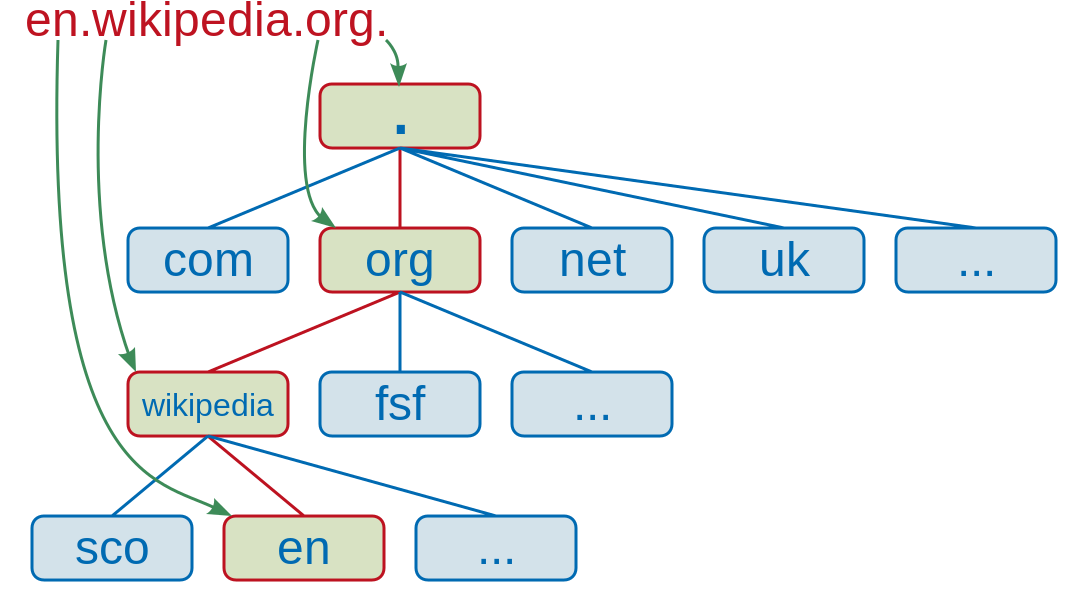
\includegraphics[width=0.8\textwidth]{obrazky-figures/DNS_schema.png}
    \caption{Hierarchická struktura systému DNS.}
    \label{fig:dns_schema}
\end{figure}

\subsection{Funkce internetových domén}
Doménová jména hrají zásadní roli v~uspořádání a fungování moderního internetu. Slouží jako lidsky čitelný prostředník mezi uživateli a IP adresami, což umožňuje snadnou navigaci a přístup k~online službám. Zároveň poskytují klíčovou infrastrukturu pro širokou škálu internetových funkcí, od webového hostingu přes e-mailové služby až po integraci aplikací a API. Tato flexibilita však přináší i rizika spojená se zneužitím \cite{komaitis2010domain}.

Funkci domén bychom mohli shrnout do následujících bodů:
\begin{itemize}
    \item \textbf{Identifikace zdrojů} Doménová jména umožňují jednoznačnou identifikaci zdrojů na internetu, což je zásadní pro směrování dat a poskytování služeb.
    \item \textbf{Značka a identita}Domény často nesou identitu organizací, produktů nebo jednotlivců, což jim dodává hodnotu nejen z~technického, ale i z~marketingového hlediska.
    \item \textbf{Hierarchické uspořádání}Struktura doménového jména (např. subdomény, hlavní doména, TLD) podporuje efektivní organizaci a škálování internetových zdrojů.
    \item \textbf{Zprostředkování bezpečnosti} Domény hrají klíčovou roli v~implementaci bezpečnostních protokolů, jako je TLS/SSL, které zajišťují šifrovanou komunikaci.
\end{itemize}





\subsection{Maligní domény}
Maligní domény, definované ve širším kontextu, jsou webové domény vytvořené s~účelem působit škodu nebo získávat finanční prospěch na úkor uživatelů internetu. Tyto domény jsou často zásadní součástí kybernetických hrozeb, jako jsou distribuce malware, phishingové útoky a další formy podvodné činnosti. Identifikace a monitorování maligních domén je nezbytné pro prevenci kybernetických útoků a zajištění bezpečnosti uživatelů internetu \cite{antonakakis2017understanding}.

Typickým příkladem jsou phishingové domény, které imitují důvěryhodné služby, např. \texttt{secure-login-bank.com} nebo \texttt{paypal-verification.net}, přičemž cílem je oklamat uživatele k~zadání citlivých údajů. Tyto názvy často využívají sociální inženýrství, kombinují důvěryhodně znějící slova a využívají domén nejvyšší úrovně, které jsou levně dostupné.

Maligní domény nejsou jasně definovanou kategorií, ale existují spíše na škále, které se liší účelem a metodami. Pro účely jednoduché klasifikace můžeme doménová jména rozdělit do následujících hlavních kategorií založených na jejich účelu a charakteristikách:

\begin{enumerate}
    \item \textbf{Phishingové domény:} Tyto domény jsou navrženy tak, aby napodobovaly legitimní webové stránky s~cílem získat citlivé informace, jako jsou přihlašovací údaje a finanční informace uživatelů \cite{moore-clayton}.
    \item \textbf{Domény distribuující malware:} Tento typ domén je používán k~šíření škodlivého softwaru, jako jsou viry, červi nebo trojské koně, často prostřednictvím infikovaných souborů nebo skriptů \cite{provos2007virtual}.
    \item \textbf{Domény propagující nežádoucí reklamu:} Tyto domény obvykle distribuují nevyžádanou nebo klamavou reklamu. Nicméně, je důležité si uvědomit, že hranice mezi maligními a benigními reklamními doménami je často nejasná. Ne všechny reklamní domény jsou nutně maligní, ačkoli některé mohou být použity pro škodlivé účely \cite{thomas2015ad}.
    \item \textbf{DGA domény (Domain Generation Algorithms):} Tyto domény jsou generovány algoritmicky a často slouží k~řízení botnetů. DGA domény jsou zásadní pro komunikaci mezi centrálním řídícím serverem a jednotlivými infikovanými zařízeními v~botnetu. Typickým rysem je jejich zdánlivě náhodný vzhled, který ztěžuje jejich odhalení tradičními filtračními mechanismy \cite{plohmann2016comprehensive}. 
    
\end{enumerate}

Abstraktně lze u~maligních domén vypozorovat několik charakteristik, včetně neobvyklých vzorců přístupu, podezřelého chování v~síťovém provozu, a často i využití zaměňujících nebo podobných názvů k~legitimním doménám, což umožňuje zastírat jejich pravou identitu a účel \cite{perdisci2009detection}.



\subsection{Phishing}
Phishingové domény jsou typem maligních domén zaměřených na získávání citlivých informací od uživatelů předstíráním důvěryhodného zdroje. Tyto domény často imitují webové stránky bank, e-mailových služeb nebo jiných online platforem s~cílem získat přihlašovací údaje, osobní informace nebo finanční data. Charakteristickým rysem těchto domén je vytváření vizuálně identických replik legitimních stránek. Detekce phishingových domén může být založena na analýze obsahu, porovnání s~databázemi známých phishingových stránek a sledování neobvyklého chování návštěvníků \cite{moore-clayton}.

\subsection{Malware}
Maligní domény spojené s~distribucí malwaru slouží k~šíření škodlivých programů a virů. Tyto domény mohou obsahovat infikovaný software, který je stažen nebo spuštěn návštěvníkem stránky. Malware může být použit pro odcizení dat, sledování chování uživatelů nebo pro vytvoření tzv. botnetů. Typické pro malwarové domény je často krátká životnost a rychlá změna názvu nebo obsahu k~minimalizaci odhalení. Detekce malwarových domén vyžaduje analýzu souborů, síťového provozu a dynamického chování k~identifikaci podezřelých aktivit \cite{provos2007virtual}.

\subsection{Botnet}
Domény spojené se sítěmi botnet představují centrální kontrolní body pro sítě infikovaných počítačů (botů). Tyto domény slouží k~řízení botů a sběru dat z~infikovaných zařízení. Sítě botnet jsou často využívány k~masivnímu rozesílání spamu, útokům typu DDoS nebo k~distribuci dalšího malwaru. Charakteristickým rysem botnetových domén je snaha o~udržení stability a dostupnosti pro správu botů. Detekce botnetových domén zahrnuje analýzu síťového provozu, sledování podezřelých komunikačních vzorů a identifikaci charakteristik botů \cite{plohmann2016comprehensive}.

\subsection{DGA (Domain Generation Algorithms)}
DGA domény jsou generovány algoritmicky a slouží primárně k~řízení botnetů. Charakteristické pro DGA domény je jejich náhodná generace, krátká životnost a použití jako prostředků pro komunikaci s~command-and-control servery. Tyto domény jsou klíčové pro skryté předávání pokynů a informací mezi sítěmi botnet a jejich řídícími servery, často slouží také jako proxy pro zabezpečení anonymity a komplikaci sledování \cite{yadav2010detecting}.


\subsubsection{Detekce a Charakteristiky Maligních Domén}
Detekce maligních domén je klíčovým prvkem v~kybernetické bezpečnosti. Analytici se zaměřují na specifické charakteristiky domén, které mohou indikovat škodlivost. Mezi tyto charakteristiky patří podezřelé znaky v~doménovém jméně, neobvyklé kombinace písmen a čísel, nečekané změny v~chování domény a další.

Různé metody detekce zahrnují analýzu DNS provozu, sledování historie domén, a využití strojového učení a umělé inteligence pro identifikaci vzorců a anomálií. Efektivní detekce vyžaduje komplexní přístup a neustálou aktualizaci technik pro odhalení stále se vyvíjejících metod kybernetických hrozeb \cite{bilge2011exposure}.

Následující části této kapitoly podrobně rozebírají jednotlivé metody detekce a strategie pro účinnou identifikaci maligních domén v~dynamickém prostředí internetu.

Klasifikace maligních domén vyžaduje systematický přístup k~identifikaci indikátorů jejich škodlivé povahy. Kromě specifických ukazatelů pro phishing, malware a botnety existují obecné indikátory, které lze využít při analýze a klasifikaci těchto domén:

\begin{itemize}
    \item \textbf{Krátká životnost:} Maligní domény často existují jen krátkou dobu, aby minimalizovaly riziko odhalení. Sledování délky existence domény může být klíčovým ukazatelem \cite{zhauniarovich2018survey}.
    
    \item \textbf{Neobvyklé chování:} Abnormální chování domény, jako například neobvyklý provoz, může být známkou škodlivé aktivity. Analýza chování může odhalit podezřelé vzory \cite{bilge2011exposure}.
    
    \item \textbf{Častá změna obsahu nebo názvu:} Maligní domény se často snaží zůstat v~krytu tím, že často mění svůj obsah nebo název. Sledování těchto změn může představovat klíčový indikátor \cite{zhauniarovich2018survey}.
    
    \item \textbf{Nízká reputace:} Využívání reputačních databází pro hodnocení domén může poskytnout informace o~tom, zda byla doména dříve spojena s~nekalými praktikami \cite{antonakakis2010building}.
    
    \item \textbf{Podezřelé WHOIS informace:} Nepravdivé nebo anonymní údaje v~registračních informacích (WHOIS) mohou být indikátorem snahy skrýt pravé záměry domény \cite{bilge2011exposure}.
    
    \item \textbf{Špatně definovaná struktura:} Nedostatek jasné struktury nebo nekonzistence v~obsahu domény může naznačovat, že byla vytvořena za účelem škodlivé činnosti \cite{zhauniarovich2018survey}.
\end{itemize}

\section{Současné přístupy detekce maligních domén}

Jak již bylo řečeno, internetové domény jsou často využívány k~šíření malwaru, phishingovým útokům nebo jako nástroje pro řízení botnetů \cite{provos2007virtual, bilge2011exposure}. V~reakci na tento problém byly vyvinuty různé techniky, od tradičních černých listin až po pokročilé metody strojového učení a hlubokých neuronových sítí \cite{ma2011learning, torroledo2018hunting}. Moderní metody, jako je analýza DNS dotazů nebo analýza algoritmů DGA, prokazují vysokou účinnost při identifikaci nově vznikajících hrozeb \cite{bilge2011exposure, plohmann2016comprehensive}.




\subsection{Černé listiny} \label{blacklists}
Černé listiny představují základní nástroj pro detekci maligních domén, sestavovaný a udržovaný různými organizacemi. Tento přístup využívá ruční hlášení uživateli, automatizované monitorování a integraci znalostí třetích stran \cite{ovi}. Ačkoli jsou černé listiny efektivní a snadno implementovatelné, mohou být velmi omezené v~případě nově vznikajících hrozeb.

Moore a Clayton ve své studii zkoumají účinnost odstranění phishingových webů, což je přístup úzce spojený s~používáním černých listin. \cite{moore-clayton} Provos et al. se zaměřují na analýzu malwaru šířeného prostřednictvím webových stránek, což je klíčové pro pochopení, jak černé listiny pomáhají v~identifikaci škodlivých domén. \cite{provos-etal} Thomas et al. poskytují pohled na reklamní taktiky využívající maligní domény, což je oblast, kde černé listiny mohou hrát roli v~detekci a prevenci \cite{thomas2015ad}.



\subsection{Lexikální analýza}
Lexikální analýza maligních domén se zaměřuje na analýzu a klasifikaci textu doménových jmen. Výzkumy v~této oblasti představují lehký, ale efektivní přístup k~proaktivní detekci a kategorizaci škodlivých URL. Algoritmy strojového učení, jako jsou Random Forest, K-Nearest Neighbour (KNN), Decision Tree a Extra Tree Classifier, byly použity k~analýze více než 700 000 URL, přičemž byly klasifikovány do kategorií jako benigní, defacement, malware a phishing. Bylo zjištěno, že použití pouze 15 nejdůležitějších lexikálních vlastností je dostačující a nezbytné pro klasifikaci těchto kategorií \cite{ma2011learning,perdisci2012url}.

Důležitým aspektem této metody je rozdělení výsledků klasifikace do dvou částí: a) výsledky klasifikace různými algoritmy strojového učení založenými na lexikálních vlastnostech; a b) matice záměn a AUC-ROC křivka pro dva nejlepší algoritmy - Random Forest a Extra Tree. Tento přístup poskytuje spolehlivou a užitečnou metodu pro detekci nových typů útoků, zejména v~případě, kdy je k~dispozici velké množství URL \cite{sahoo2017malicious,srinivasan2018detecting}.

\subsection{Využití kombinovaných CNN-GRU-Attention modelů}

Tento přístup k~detekci maligních domén spočívá v~použití kombinace konvolučních neuronových sítí (CNN), rekurentních neuronových sítí s~jednotkami Gated Recurrent Unit (GRU) a Attention mechanismů. Tento model je schopen efektivně zpracovávat jak prostorové vlastnosti (pomocí CNN), tak i časové závislosti v~datech (pomocí GRU). Attention mechanismus pak umožňuje modelu lépe se zaměřit na relevantní části dat, což vede k~větší přesnosti při klasifikaci domén. Tento přístup nabízí lepší výsledky než tradiční metody, protože dokáže zachytit složitější vzory a vztahy v~datech \cite{cnn_gru_attention}.

\subsection{Adopce strojového učení pro podporu detekce maligních domén}

Tento přístup zahrnuje využití různých algoritmů strojového učení pro klasifikaci domén jako maligních nebo neškodných. Zahrnuje tvorbu a analýzu rozsáhléh datové sady domén, které jsou předem klasifikovány jako maligní nebo benigní. Výzkum zahrnuje aplikaci různých algoritmů strojového učení, jako jsou Naive Bayes, Support Vector Machines, Decision Trees, Random Forests, Logistic Regression a Neural Networks, na tuto datovou sadu. Výsledky ukazují, že některé algoritmy dosahují přesnosti klasifikace mezi 0.75  a 0.92, přičemž čas potřebný pro klasifikaci nové domény se pohybuje od několika sekund do více než hodiny \cite{ml_malicious_domains}.


\subsection{Analýza DNS dotazů pomocí strojového učení}

Tento přístup k~detekci maligních domén spočívá v~analýze DNS dotazů s~využitím metod strojového učení. Metoda se zaměřuje na extrakci a analýzu charakteristik DNS dotazů, jako jsou počet dotazů, časové intervaly mezi dotazy, a typy požadovaných záznamů. Strojové učení je následně využito k~detekci anomálií v~těchto charakteristikách, které mohou indikovat maligní aktivity. Algoritmy jako Random Forest, Support Vector Machines nebo neurální sítě jsou aplikovány na data, což umožňuje identifikaci potenciálně škodlivých domén s~vysokou přesností. Tento přístup je efektivní zejména v~detekci nových a neznámých hrozeb, které nejsou zahrnuty v~existujících černých listinách nebo databázích \cite{dns_query_analysis_ml}.

\subsection{Detekce phishingových certifikátů pomocí hlubokých neuronových sítí}
Vzhledem k~nárůstu využití šifrované komunikace v~rámci TLS certifikátů kybernetickými útočníky, kteří často zneužívají certifikáty k~zakrývání phishingových aktivit, se objevily nové techniky zaměřené na detekci škodlivých certifikátů pomocí hlubokých neuronových sítí. Torroledo a kol. (2018) navrhli model, který analyzuje obsah TLS certifikátů a identifikuje škodlivé vzorce využívané útočníky. Systém dosahuje přesnosti 94.87 \%  při detekci malwarových certifikátů a 88.64\% při detekci phishingových certifikátů. Tento model využívá kombinace klasifikačních prvků extrahovaných z~certifikátů a schopnosti hlubokých neuronových sítí analyzovat textová data obsažená v~certifikátech, čímž umožňuje odhalit i skryté vzorce v~chování útočníků. Tento přístup ukazuje na potenciál hlubokého učení v~oblasti kybernetické bezpečnosti a na jeho efektivitu v~porovnání s~tradičními metodami, jako je podpora vektorových strojů (SVM), kterou tento model převyšuje přesností o~7\% \cite{torroledo2018hunting}.

\subsection{Porovnání metod strojového učení pro detekci phishingu}
Další výzkum v~oblasti detekce phishingových útoků se zaměřuje na porovnání různých metod strojového učení, včetně logistické regrese, rozhodovacích stromů, bayesovských aditivních regresních stromů (BART), náhodných lesů a neuronových sítí. Studie Abu-Nimeha a kol. (2007) testuje predikční přesnost těchto metod na datové sadě obsahující phishingové a legitimní e-maily, přičemž jednotlivé metody vykazují různé úrovně přesnosti. Například náhodné lesy vykazují nejlepší výkonnost s~přesností 90,24 \% při vážení chyb na základě penalizace falešně pozitivních detekcí \cite{abuNimeh2007comparison}. Tato studie zdůrazňuje význam pečlivého výběru klasifikátorů pro detekci phishingových aktivit, protože různé přístupy poskytují různé úrovně vyváženosti mezi falešně pozitivními a falešně negativními výsledky. Tento přístup poskytuje základní vhled do toho, jak mohou různé modely přispět k~účinné detekci phishingových útoků na základě specifických charakteristik phishingových zpráv a vzorců chování útočníků \cite{abuNimeh2007comparison}.

\subsection{Detekce pomocí lexikální analýzy a síťových aktivit}

Amit Kumar a Soumyadev Maity představili hybridní přístup k~identifikaci a kategorizaci škodlivých URL pomocí kombinace lexikálních vlastností a síťových aktivit. Ve svém výzkumu použili rozsáhlou datovou sadu obsahující více než 700 000 URL, které byly klasifikovány do kategorií benigní, phishing, malware a defacement. Analyzované vlastnosti zahrnovaly délku URL, délku hostname, entropii a další metriky odvozené z~textu URL.

Byly testovány klasifikační metody jako Random Forest, K-Nearest Neighbors, Decision Tree a Extra Tree Classifier. Nejlepších výsledků dosáhly algoritmy Random Forest a Extra Tree Classifier s~přesností až 93 \%. Tento přístup prokázal, že kombinace lexikálních vlastností a síťových aktivit umožňuje přesnou a rychlou detekci škodlivých URL. Autoři zdůraznili, že jejich metoda je obzvláště efektivní při analýze rozsáhlých datových sad a může být implementována jako klíčový nástroj pro boj proti phishingovým a malwarovým útokům \cite{kumar}.


\section{Srhnutí současných přístupů a jejich přínosu}

Na základě analýzy jednotlivých metod lze konstatovat, že žádný přístup není univerzální. Tradiční metody, jako jsou černé listiny, jsou rychlé a snadno implementovatelné, avšak jejich efektivita je omezena u~nově vznikajících hrozeb. Na druhé straně pokročilé metody strojového učení nabízejí vyšší přesnost a adaptabilitu, avšak vyžadují větší výpočetní výkon a pečlivě připravené datové sady.

Integrace více přístupů do jednoho komplexního systému detekce maligních domén se jeví jako nejefektivnější strategie. Kombinace blacklistingu s~analýzou DNS provozu a využitím modelů hlubokého učení může výrazně snížit míru falešně pozitivních i falešně negativních detekcí a zvýšit schopnost systému reagovat na nové typy hrozeb.


\subsection{Využití rozsáhlých dat pro detekci maligních domén}

S~nárůstem počtu dostupných dat a pokročilých metod jejich analýzy se využití rozsáhlých datových sad a bohatých vektorů příznaků stalo klíčovým přístupem k~efektivní detekci maligních domén. Moderní algoritmy dokáží těžit z~kombinace různorodých zdrojů dat, jako jsou DNS dotazy, WHOIS informace, síťové aktivity, a vlastnosti získané lexikální analýzou \cite{bilge2011exposure, ma2011learning}.

\paragraph{Rozsáhlá data při klasifikaci}
Rozšířené vektory příznaků zahrnují kombinaci tradičních metrik, jako je délka doménového jména, entropie nebo počet poddomén, spolu s~pokročilými vlastnostmi získanými z~dynamické analýzy, např. vzorce síťového provozu nebo doba existence domény. Tato rozmanitost umožňuje pokročilým modelům strojového učení, včetně hlubokých neuronových sítí, zachytit komplexní vzory a vztahy, které by tradiční metody mohly přehlédnout \cite{cnn_gru_attention, bilge2011exposure}.

Přístup spočívající v~maximalizaci vektoru příznaků byl prokázán jako účinný zejména při využití pokročilých modelů, jako jsou konvoluční neuronové sítě (CNN) a modely využívající mechanismy pozornosti (Attention). Například modely kombinující CNN a rekurentní neuronové sítě (GRU) ukázaly, že čím širší spektrum vlastností je analyzováno, tím přesnější je detekce \cite{cnn_gru_attention}.

\paragraph{Výhody a optimalizace}
Použití rozsáhlých datových sad nejen zlepšuje přesnost modelů, ale také umožňuje efektivní detekci nově vznikajících a neznámých hrozeb. Analýzy DNS provozu ukázaly, že data o~časových intervalech mezi dotazy nebo geografické distribuci žádostí mohou poskytnout klíčové informace o~anomálních vzorcích chování \cite{dns_query_analysis_ml}.

Optimalizace vektoru příznaků zahrnuje výběr relevantních vlastností a eliminaci redundantních nebo irelevantních informací. Metody jako PCA (Principal Component Analysis) nebo výběr na základě informačního zisku jsou často využívány pro zlepšení efektivity bez kompromisů na přesnosti \cite{ma2011learning, bilge2011exposure}.

Tento přístup založený na rozsáhlých datových vektorech přináší významné výhody pro detekci maligních domén. Kombinace různorodých datových zdrojů s~pokročilými analytickými metodami umožňuje vytvářet robustní modely schopné adaptace na dynamicky se měnící hrozby.


\subsection{Vývoj v~oblasti detekce maligních domén}

Oblast detekce maligních domén zaznamenala v~posledních dekádách významný vývoj, který odráží rostoucí sofistikovanost kybernetických hrozeb a pokrok v~oblasti analýzy dat. Počáteční přístupy byly založeny na statických černých listinách, které se ukázaly jako účinné proti známým hrozbám \cite{provos2007virtual, moore-clayton}. Tyto přístupy však byly postupně překonány dynamikou moderních útoků, jež využívají rychlé změny a maskování doménových jmen, což vedlo k~rozvoji metod strojového učení.

Metody založené na strojovém učení, jako je lexikální analýza doménových jmen, přinesly významnou změnu díky schopnosti rychle a přesně klasifikovat velké množství URL \cite{ma2011learning, perdisci2012url}. Další pokroky zahrnovaly analýzu DNS provozu, která umožnila identifikaci anomálních vzorců v~síťovém provozu, a detekci pomocí TLS certifikátů, která odhalila skryté vzory chování útočníků \cite{dns_query_analysis_ml, torroledo2018hunting}.

V~posledních letech se do popředí dostávají hluboké neuronové sítě, jako jsou modely CNN a GRU s~mechanizmy pozornosti (Attention), které dokáží efektivně zachytit prostorové i časové závislosti v~datech. Tyto modely dosahují vysoké přesnosti při detekci nových typů hrozeb \cite{cnn_gru_attention}. Například model Torroledo a kol. dosáhl přesnosti 94.87\% při detekci malwarových certifikátů \cite{torroledo2018hunting}.

Dalším klíčovým trendem je integrace více zdrojů dat, jako jsou DNS záznamy, WHOIS informace, síťové aktivity a vlastnosti domén. Tyto multidimenzionální přístupy, často implementované prostřednictvím složených modelů, zvyšují robustnost detekčních systémů a umožňují lepší reakci na nově vznikající hrozby \cite{bilge2011exposure, abuNimeh2007comparison}.

Vývoj v~této oblasti ukazuje, že budoucnost detekce maligních domén leží v~kombinaci rychlosti, přesnosti a adaptivních schopností, což umožňuje efektivní boj proti stále sofistikovanějším kybernetickým hrozbám.





\chapter{Zdroje dat a jejich zpracování}
\label{chapter:3}

Tato kapitola bude věnována zdrojům dat internetových domén a jejich zpracování, které jsou nezbytné pro efektivní detekci a analýzu maligních domén. Pochopení a správná aplikace metod zpracování dat jsou klíčové pro identifikaci a klasifikaci škodlivých domén. Kapitola poskytne přehled o~různých typech dat, které jsou k~dispozici pro výzkum a praxi v~oblasti kybernetické bezpečnosti.

První část kapitoly se zaměří na základní a univerzální zdroje dat, následně budou představeny zdroje pro škodlivé domény a na závěr bude rozebrána příprava dat. 




\section{Základní zdroje doménových dat}

Zdroje dat poskytují klíčové informace potřebné pro analýzu a hodnocení domén z~hlediska jejich důvěryhodnosti či potenciální škodlivosti. Dále budou rozebrány především protokoly DNS, WHOIS, RDAP, TLS certifikáty a geolokační data.


\subsection{Domain Name System (DNS)}
Jak bylo uvedeno v~sekci \ref{DNS_section}, Domain Name System (DNS) je zásadní protokol internetové infrastruktury, jehož hlavním úkolem je převod doménových jmen na odpovídající IP adresy. DNS využívá hierarchickou a decentralizovanou strukturu, která umožňuje efektivní směrování uživatelských požadavků na cílové servery. Tento systém je nezbytný pro správné fungování internetu a tvoří základní vrstvu propojení mezi uživateli a zdroji na webu \cite{postel1983domain2}.

DNS uchovává informace o~doménách ve formě tzv. \emph{Resource Records} (RR), které poskytují různé typy údajů o~konfiguraci a funkcích jednotlivých domén. Mezi nejvýznamnější patří:
\begin{itemize}
    \item \textbf{A~a AAAA záznamy}: Slouží k~mapování domén na IPv4 nebo IPv6 adresy, což je základní funkce DNS pro zajištění dostupnosti online zdrojů.
    \item \textbf{MX záznamy}: Uvádějí e-mailové servery odpovědné za zpracování pošty pro konkrétní doménu. Tyto záznamy jsou klíčové pro ochranu proti nevyžádané poště a phishingovým kampaním, protože lze analyzovat neobvyklé nebo podezřelé konfigurace.
    \item \textbf{TXT záznamy}: Umožňují ukládání volitelných textových dat, která se často využívají k~ověřování bezpečnostních mechanismů, jako jsou SPF, DKIM nebo DMARC, jež zajišťují ochranu proti spoofingu e-mailů.
    \item \textbf{CNAME záznamy}: Poskytují aliasování domén, což umožňuje mapovat více názvů na stejný server. Tato vlastnost je často využívána v~kombinaci se službami CDN (Content Delivery Network).
    \item \textbf{NS záznamy (Name Server)}: Definují autoritativní DNS servery, které jsou odpovědné za konkrétní doménu. Tyto záznamy určují, které servery mají být dotazovány pro získání informací o~doméně.
    \item \textbf{SOA záznamy (Start of Authority)}: Obsahují základní informace o~doméně, například primární DNS server, e-mail administrátora a intervaly aktualizací záznamů. Jsou nezbytné pro správnou správu zón.
    \item \textbf{PTR záznamy (Pointer)}: Používají se při reverzním DNS, kde je IP adresa mapována zpět na doménové jméno. Tato funkce je užitečná například při konfiguraci e-mailových serverů nebo detekci zneužití IP adres.
    \item \textbf{SRV záznamy (Service)}: Určují umístění specifických služeb, například VoIP nebo služby instant messagingu, a umožňují vyhledávání podle protokolu a priority.
    \item \textbf{CAA záznamy (Certificate Authority Authorization)}: Definují, které certifikační autority mohou vydávat TLS/SSL certifikáty pro danou doménu, čímž přispívají k~zabezpečení komunikace.
    \item \textbf{NAPTR záznamy (Naming Authority Pointer)}: Poskytují pokročilé přesměrování a jsou často využívány v~telekomunikačních aplikacích, například při překladu telefonních čísel na URI.
    \item \textbf{DNSKEY záznamy}: Obsahují veřejné klíče používané v~rámci DNSSEC (Domain Name System Security Extensions), které poskytují autentizaci DNS záznamů a chrání před podvržením.
    \item \textbf{DS záznamy (Delegation Signer)}: Používají se v~DNSSEC a obsahují hash klíče podepisujícího zónu, čímž umožňují propojení bezpečnostních klíčů mezi rodičovskou a podřízenou doménou.
\end{itemize}


\subsubsection*{Pasivní DNS (pDNS)}
Pasivní DNS (\emph{Passive DNS}) je metoda umožňující monitorování DNS provozu, přičemž zachycuje a ukládá informace o~dotazech a odpovědích mezi servery. Tento přístup přináší možnost analýzy historických dat, což je klíčové pro identifikaci vzorců zneužívání domén. Pasivní DNS poskytuje globální pohled na chování domén a odhaluje podezřelé aktivity, jako je využívání krátkodobých domén pro phishingové kampaně nebo sítě botnet \cite{silveira2021detection}.

\subsubsection*{Využití DNS při analýze domén}
Kromě své primární funkce lze DNS využít jako cenný zdroj dat pro detekci podezřelých aktivit spojených s~maligními doménami:
\begin{itemize}
    \item \emph{NXDOMAIN Responses}: Vysoký počet odpovědí označujících neexistující domény může naznačovat aktivitu malwaru nebo botnetů, které generují velké množství dotazů na domény vytvořené algoritmem DGA (\emph{Domain Generation Algorithm}) \cite{zou2019detecting}.
    \item \emph{TTL analýza}: Časté změny hodnot \emph{Time to Live} mohou indikovat použití metody \emph{Fast Flux}, kde útočníci pravidelně mění IP adresy domén za účelem zakrytí jejich skutečného umístění \cite{silveira2021detection}.
\end{itemize}


\subsection{WHOIS a RDAP}
WHOIS a RDAP (Registration Data Access Protocol) jsou dva zásadní protokoly poskytující informace o~vlastnictví, správě a stavu domén. Tyto zdroje dat hrají klíčovou roli při analýze domén, umožňují identifikaci jejich legitimity a pomáhají odhalovat potenciálně maligní aktivity \cite{shah2021rdap, campos2019rdap}.

\subsubsection*{WHOIS}
WHOIS je tradiční protokol používaný již od počátků internetu. Zajišťuje přístup k~údajům o~doménách, jako jsou informace o~registrátorovi a vlastníkovi domény, data registrace a expirace či aktuální stav domény (aktivní, pozastavená, expirovaná apod.) \cite{mockdomain}. Typicky poskytuje tyto informace:
\begin{itemize}
    \item \textbf{Identifikace registrátora a vlastníka}: Zahrnuje jméno, adresu a kontaktní informace. Tyto údaje mohou být u~některých registrů anonymizovány prostřednictvím služeb na ochranu soukromí (\emph{WHOIS Privacy}).
    \item \textbf{Časové informace}: Datum registrace, expirace a poslední aktualizace záznamu. Nově registrované domény mohou být varovným signálem pro phishingové kampaně nebo jiné škodlivé aktivity \cite{ma2009beyondblacklists}.
    \item \textbf{Stav domény}: Informace o~tom, zda je doména aktivní, pozastavená, nebo ve fázi přenosu, což může být důležité pro odhalování zneužití domény.
\end{itemize}

Ačkoli WHOIS poskytuje cenná data, jeho nevýhodou je často nejednotný formát a chybějící standardizace napříč registry \cite{campos2019rdap}. Navíc ochrana soukromí u~některých registrátorů může omezit dostupnost informací. V~důsledku těchto omezení vznikl modernější protokol RDAP.

\subsubsection*{RDAP (Registration Data Access Protocol)}
Protokol RDAP byl navržen jako standardizovaná a bezpečnější alternativa k~WHOIS. Tento protokol poskytuje strukturovaná data ve formátu JSON, což usnadňuje jejich zpracování a analýzu. RDAP zahrnuje podporu pro řízení přístupu, což znamená, že různí uživatelé mohou mít přístup k~různým úrovním detailů na základě jejich oprávnění \cite{shah2021rdap}.

\noindent Klíčové vlastnosti RDAP zahrnují:
\begin{itemize}
    \item \textbf{Strukturovaný formát}: Data jsou organizována ve formátu JSON, což umožňuje snadnou integraci s~analytickými nástroji a automatizované zpracování.
    \item \textbf{Podpora pro zabezpečení}: RDAP implementuje autentizaci a autorizaci přístupu, což chrání data před neoprávněným využitím \cite{ma2009beyondblacklists}.
    \item \textbf{Dodatečné informace}: Kromě základních údajů může RDAP poskytovat metadata, jako jsou geolokační informace, informace o~subjektech spravujících doménu či technické údaje o~DNS serverech \cite{campos2019rdap}.
\end{itemize}

RDAP umožňuje analýzu dat v~kontextu většího počtu atributů než WHOIS, což jej činí výhodným při zkoumání potenciálně škodlivých domén. Například detekce anomálních vzorců v~registracích (např. masové registrace anonymními subjekty) může být usnadněna díky transparentnějšímu přístupu ke struktuře dat.

\subsubsection*{Využití WHOIS a RDAP při analýze domén}
WHOIS a RDAP se často využívají při analýze důvěryhodnosti domén a identifikaci potenciálně maligních aktivit. Mohou odhalit:
\begin{itemize}
    \item \textbf{Podezřelé registrátory}: Některé registrátory jsou známé tím, že umožňují anonymní registrace nebo mají slabší bezpečnostní politiku \cite{shah2021rdap}.
    \item \textbf{Rychlé registrace a expirace}: Maligní domény bývají často registrovány na krátkou dobu a jejich platnost se pravidelně obnovuje nebo expirováno během krátkého období \cite{ma2009beyondblacklists}.
    \item \textbf{Geografické vzory}: Analýza země původu registrátora může odhalit oblasti spojené s~častým hostingem škodlivých domén \cite{campos2019rdap}.
\end{itemize}

WHOIS a RDAP jsou tak základními nástroji při shromažďování dat pro systémy detekce škodlivých domén, přičemž RDAP se díky své moderní infrastruktuře stává preferovanou volbou \cite{campos2019rdap}.


\subsection{TLS Certifikáty}
TLS (Transport Layer Security) certifikáty jsou klíčovou součástí infrastruktury veřejných klíčů (PKI) a zajišťují bezpečnou komunikaci mezi klienty a servery na internetu. Certifikáty založené na standardu X.509 obsahují informace o~identitě serveru, veřejném klíči a dalších parametrech nezbytných pro šifrování a autentizaci. \cite{rescorla2018tls13, cooper2008x509}

\subsubsection*{Struktura TLS certifikátu}
TLS certifikát obsahuje několik klíčových komponent, které umožňují jeho použití v~kryptografickém procesu \cite{cooper2008x509, cabforum_tls}.
\begin{itemize}
    \item \textbf{Subjekt certifikátu}: Identifikuje entitu, pro kterou byl certifikát vydán, například konkrétní doménu (\emph{Common Name, CN}) nebo organizaci. Může zahrnovat také alternativní názvy subjektu (\emph{Subject Alternative Name, SAN}) pro podporu více domén či subdomén.
    \item \textbf{Vydavatel certifikátu}: Identifikuje certifikační autoritu (CA), která certifikát vydala. Tato informace obsahuje název CA, její digitální podpis a případná rozšíření.
    \item \textbf{Veřejný klíč}: Kryptografický klíč, který je použitý při inicializaci šifrované komunikace. Veřejný klíč slouží ke šifrování dat, která může dešifrovat pouze odpovídající privátní klíč.
    \item \textbf{Sériové číslo certifikátu}: Jedinečný identifikátor certifikátu, který je přiřazen vydavatelem.
    \item \textbf{Platnost certifikátu}: Definuje časové období, během kterého je certifikát platný. Obsahuje datum a čas vydání a expirace.
    \item \textbf{Rozšíření certifikátu}: Tato část zahrnuje další informace, například omezení na specifické aplikace nebo protokoly (\emph{Key Usage}), podporu šifrovacích algoritmů či identifikaci hierarchie certifikačních autorit (\emph{Certificate Policies}).
    \item \textbf{Digitální podpis}: Podpis vytvořený certifikační autoritou, který ověřuje autenticitu certifikátu. Používá hash původního obsahu certifikátu šifrovaný privátním klíčem CA.
\end{itemize}

\subsubsection*{Funkce TLS certifikátů v~PKI}
TLS certifikáty fungují jako součást infrastruktury veřejných klíčů, která zajišťuje důvěryhodnost a bezpečnost v~rámci internetové komunikace. Tento proces zahrnuje několik klíčových kroků \cite{cooper2008x509, stallings2017cryptography}.
\begin{enumerate}
    \item \textbf{Vydání certifikátu}: Certifikační autorita (CA) po ověření identity subjektu vystaví certifikát, který obsahuje veřejný klíč a další informace o~subjektu.
    \item \textbf{Distribuce certifikátu}: Certifikát je distribuován klientům prostřednictvím protokolu TLS během procesu navazování spojení (\emph{TLS handshake}).
    \item \textbf{Validace certifikátu}: Klient při navazování spojení ověřuje podpis certifikátu proti seznamu důvěryhodných certifikačních autorit (uložených v~tzv. \emph{trust store}) a kontroluje jeho platnost (např. datum expirace a zrušení).
    \item \textbf{Použití veřejného klíče}: Veřejný klíč obsažený v~certifikátu je využit k~šifrování přenosu nebo k~ověření digitálních podpisů serveru.
\end{enumerate}

\subsubsection*{TLS Handshake a role certifikátů}
TLS handshake je proces navazování šifrovaného spojení mezi klientem a serverem. Certifikáty zde hrají klíčovou roli v~autentizaci a zabezpečení komunikace: \cite{rescorla2018tls13, stallings2017cryptography}
\begin{itemize}
    \item \textbf{Serverová autentizace}: Server poskytuje svůj certifikát klientovi, který ověřuje jeho pravost proti důvěryhodným CA.
    \item \textbf{Sdílení šifrovacích parametrů}: Na základě informací z~certifikátu a zvolených algoritmů je mezi klientem a serverem vygenerován šifrovací klíč pro zabezpečení další komunikace.
    \item \textbf{Volitelné ověření klienta}: V~některých scénářích může být použit i klientský certifikát pro oboustrannou autentizaci.
\end{itemize}

\subsubsection*{Typy TLS certifikátů}
TLS certifikáty mohou být kategorizovány podle úrovně validace a použití \cite{cabforum_tls, barnes2016multi}.
\begin{itemize}
    \item \textbf{Domain Validation (DV)}: Ověřuje vlastnictví domény, ale neposkytuje informace o~organizaci. DV certifikáty jsou rychle vydávány a jsou nejčastěji využívány menšími weby \cite{barnes2016multi}.
    \item \textbf{Organization Validation (OV)}: Ověřuje vlastnictví domény i identitu organizace. OV certifikáty zajišťují větší důvěryhodnost a jsou vhodné pro organizace poskytující citlivé služby, například finanční instituce \cite{cabforum_tls}.
    \item \textbf{Extended Validation (EV)}: Poskytuje nejvyšší úroveň důvěry, zahrnuje přísné ověření organizace a je vizuálně zvýrazněn v~prohlížečích (např. zelený adresní řádek u~starších prohlížečů) \cite{cabforum_tls}.
    \item \textbf{Wildcard certifikáty}: Platí pro doménu a všechny její subdomény. Jsou vhodné pro organizace, které potřebují zabezpečit větší množství subdomén \cite{barnes2016multi}.
    \item \textbf{Multi-Domain (SAN) certifikáty}: Umožňují zabezpečení více domén v~jednom certifikátu. Tento typ je využíván například v~prostředích s~virtualizací nebo pro služby využívající více aliasů \cite{cabforum_tls}.
\end{itemize}


\subsection{Geolokační informace}
Geolokační data představují klíčový zdroj informací pro analýzu síťových aktivit a bezpečnostních hrozeb. Tato data lze odvodit z~IP adres serverů a klientů, přičemž poskytují informace o~jejich geografické poloze, jako je země, město, region nebo dokonce přibližné GPS souřadnice. Geolokační informace lze získat z~následujících zdrojů:


\begin{itemize}
    \item \textbf{Databáze geolokací IP adres}: Služby, jako je MaxMind GeoIP, IP2Location nebo RIPE NCC, nabízejí pravidelně aktualizované databáze, které mapují IP adresy na geografické lokace \cite{geolocation_maxmind, ip2location_service}.
    \item \textbf{WHOIS záznamy}: Informace o~registraci IP adres, poskytované regionálními internetovými registry (např. ARIN, RIPE, APNIC), mohou obsahovat údaje o~geografické oblasti registrace \cite{arin_whois}.
    \item \textbf{Pasivní DNS}: Kombinace dat o~doménách a jejich IP adresách umožňuje mapování vztahů mezi doménami a jejich geografickou distribucí \cite{silveira2021detection}.
\end{itemize}

\subsubsection*{Přesnost geolokačních dat}
Přesnost geolokačních dat závisí na několika faktorech:
\begin{itemize}
    \item \textbf{Úroveň podrobnosti}: Přesnost se může pohybovat od zjištění země nebo regionu (většinou přesné na více než 95 \%) až po lokalizaci na úroveň města, kde přesnost může klesnout na 50--70~\% \cite{huang2017geolocation}.
    \item \textbf{Typ IP adresy}: Přesnost je obecně vyšší u~statických IP adres než u~dynamických, které mohou být přidělovány do různých geografických oblastí.
    \item \textbf{Proxy a VPN}: Použití proxy serverů, VPN nebo cloudových služeb může zkreslit geolokační data a naznačovat falešné umístění \cite{mcpherson2009vpn}.
    \item \textbf{Aktualizace databází}: Četnost aktualizací geolokačních databází ovlivňuje aktuálnost a přesnost informací.
\end{itemize}


I~přes široké využití mají geolokační data své limity, které ovlivňují jejich přesnost a spolehlivost. Jedním z~hlavních problémů je nejasné umístění cloudových služeb. Poskytovatelé, jako jsou AWS nebo Google Cloud, často využívají geograficky distribuované IP adresy, což výrazně komplikuje přesnou lokalizaci serverů a dalších zdrojů. Další výzvu představují mobilní sítě, kde operátoři obvykle přidělují IP adresy na základě logiky své sítě, nikoli podle fyzického umístění uživatele. To může vést k~významným rozdílům mezi skutečnou polohou uživatele a místem, které geolokační databáze indikuje. Kromě toho mohou geolokační data zkreslovat útočníci, kteří využívají technologie, jako jsou proxy servery nebo VPN, k~zakrytí své skutečné polohy. Tyto metody umožňují vytvořit falešnou geografickou stopu, která může zmást detekční systémy a ztížit analýzu \cite{mcpherson2009vpn}.





\section{Zdroje dat pro maligní domény}
Veškeré výše zmíněné zdroje dat, jako jsou DNS, WHOIS, RDAP nebo TLS certifikáty, poskytují cenné informace pro analýzu domén. Tyto zdroje umožňují získat široké spektrum atributů, které lze využít při klasifikaci domén. Nicméně, aby bylo možné doménu označit jako maligní, je klíčové mít k~dispozici informace o~její škodlivosti. Tyto informace, označované často jako \emph{ground truth}, slouží jako základ pro trénování a vyhodnocování modelů. Následující sekce se věnují zdrojům, které poskytují informace o~škodlivých doménách, jako jsou zdrojová data platformy MISP a černé listiny.

\subsection{MISP}
MISP (\emph{Malware Information Sharing Platform}) je platforma pro sdílení informací o~kybernetických hrozbách. Tato platforma umožňuje bezpečnostním týmům a organizacím sdílet indikátory kompromitace (\emph{Indicators of Compromise, IoC}), mezi které patří informace o~škodlivých doménách, IP adresách, hashe souborů a dalších entitách. Zdrojová data platformy MISP jsou sestavována na základě údajů od různých organizací, zahrnujících bezpečnostní společnosti, výzkumné týmy a národní kybernetické agentury \cite{wagner2016misp}.

\noindent Zdrojová data platformy MISP poskytují následující klíčové informace:
\begin{itemize}
    \item \textbf{Detailní metadata o~škodlivých doménách}: Obsahují informace o~typu hrozby, čase detekce, původu a dalších relevantních atributech.
    \item \textbf{Kontext hrozeb}: Například informace o~tom, zda je doména spojena s~phishingovou kampaní, šířením malwaru nebo provozem botnetů.
    \item \textbf{Automatizovaná integrace}: Díky podpoře standardizovaných formátů, jako STIX nebo OpenIOC, lze data snadno integrovat do systémů detekce a reakce na incidenty (SIEM).
\end{itemize}

\noindent Zdrojová data platformy MISP jsou užitečná zejména při průběžné aktualizaci datových sad a obohacení modelů pro detekci maligních domén o~aktuální informace o~hrozbách \cite{alexander2019misp}. 


\subsubsection{Využití bezpečnostních feedů}
Využití MISP zahrnuje integraci s~různými bezpečnostními nástroji a systémy, jako jsou SIEM systémy (Security Information and Event Management), síťové senzory, firewally a další nástroje pro prevenci a detekci hrozeb. Díky MISP lze tyto nástroje konfigurovat tak, aby automaticky reagovaly na aktuální informace, což umožňuje rychlou reakci na nově identifikované hrozby \cite{wagner2016misp}.

\subsubsection{Software a Technologie}
MISP poskytuje API (Application Programming Interface), které umožňuje snadnou integraci s~různými bezpečnostními řešeními. Díky této funkcionalitě je MISP často integrován s~dalšími nástroji a platformami, jako jsou Threat Intelligence Platforms (TIP), což umožňuje komplexní správu a analýzu hrozeb. Kromě toho MISP podporuje různé formáty pro sdílení informací, včetně STIX/TAXII, což umožňuje širší kompatibilitu s~různými systémy a standardy \cite{misp2020platform}.

\subsection{Černé listiny}
Černé listiny (\emph{blacklists}) představují další zásadní zdroj informací o~škodlivých doménách. Jak je popsáno v~sekci \ref{blacklists}, jedná se o~seznamy udržované různými organizacemi a automatizovanými systémy, které identifikují známé škodlivé domény. Tyto seznamy jsou často sestavovány na základě ručního hlášení uživatelů, automatizovaného monitorování a analýzy škodlivých aktivit. Mezi nejznámější černé listiny patří například Google Safe Browsing, PhishTank nebo Spamhaus \cite{provos-etal, moore-clayton, thomas2015ad}.

Černé listiny jsou užitečné nejen při identifikaci známých hrozeb, ale také jako základ pro \emph{ground-truth verifikaci} (viz kapitola \ref{pravda}). Slouží k~validaci domén označených jako maligní a pomáhají zajistit spolehlivost datových sad. Nicméně jejich omezení spočívají v~neschopnosti detekovat nově vznikající hrozby nebo hrozby, které se vyhýbají běžným detekčním metodám.


\subsubsection{VirusTotal API}
VirusTotal je populární online služba, která kombinuje více než 70 antivirových enginů a bezpečnostních nástrojů pro analýzu souborů, URL a domén. Poskytuje podrobné informace o~škodlivých aktivitách spojených s~analyzovanými objekty. VirusTotal API umožňuje přístup k~této službě prostřednictvím automatizovaných skriptů a je užitečné jak pro jednotlivé analýzy, tak pro hromadné zpracování datových sad. \cite{virtotal}

\paragraph{Funkce VirusTotal API}
VirusTotal API nabízí následující klíčové funkce: \cite{virtotal}
\begin{itemize}
    \item \textbf{Hodnocení domén}: VirusTotal poskytuje skóre založené na počtu detekcí jednotlivých antivirových enginů, což pomáhá rychle určit, zda je doména maligní.
    \item \textbf{Metadata o~doménách}: Služba poskytuje informace o~IP adresách, DNS záznamech, TLS certifikátech a dalších atributech spojených s~analyzovanou doménou.
    \item \textbf{Historické údaje}: Umožňuje analyzovat historické chování domén, což je užitečné při sledování trendů a dlouhodobých aktivit.
\end{itemize}

\paragraph{Využití VirusTotal API při verifikaci}
VirusTotal API hraje klíčovou roli při \emph{ground-truth verifikaci} (viz kapitola \ref{pravda}). V~rámci tohoto procesu byly všechny analyzované domény porovnány s~databázemi VirusTotal, což umožnilo víceúrovňové hodnocení. Pomocí tohoto API byly získány informace, které byly následně využity pro označení domén jako benigních nebo maligních. \cite{petr}




\section{Transformace dat}
Vzhledem k~povaze a komplexnosti dat internetových domén je klíčové zvolit správné transformace dat, které umožní efektivní klasifikaci. Následuje několik navrhovaných transformací a metod, které by mohly být použity:

\begin{itemize}
    \item \textbf{Normalizace:} Mnoho atributů, jako jsou počty DNS záznamů nebo délky IP prefixů, může mít různé rozsahy hodnot. Normalizace těchto hodnot pomůže zlepšit výkon klasifikačních algoritmů.

    \item \textbf{Kódování kategoriálních proměnných:} Některé atributy, jako jsou typy DNS záznamů, jsou kategoriální. Použití technik jako one-hot encoding nebo label encoding může převést tyto atributy na číselný formát vhodný pro strojové učení.

    \item \textbf{Redukce dimenzionality:} Vzhledem k~vysokému počtu atributů může být užitečné aplikovat techniky jako hlavní komponentní analýza (PCA) pro redukci dimenzionality a zvýraznění nejvýznamnějších vlastností.

    \item \textbf{Vytvoření nových atributů:} Můžeme vytvářet nové atributy (feature engineering) z~existujících dat, například výpočet entropie názvů domén, což může být indikátorem phishingové aktivity.
\end{itemize}

\section{Zpracování dat v~projektu FETA}

Transformace dat hraje klíčovou roli při přípravě vstupů pro strojové učení, zejména v~oblasti detekce maligních domén. Tato část práce vznikla v~rámci řešení výzkumného projektu \textbf{FETA -- Flow-based Encrypted Traffic Analysis} (kód \textbf{VJ02010024}), který je financován Ministerstvem vnitra ČR. Projekt se zaměřuje na vývoj metod detekce hrozeb ve šifrovaném síťovém provozu pomocí strojového učení a analýzy síťových toků. 

V~této sekci jsou představeny tři významné přístupy které byly využity v~rámci řešení projektu: systém A. Horáka, P. Pouče a O. Ondryáše. Všechny přístupy se zaměřují na optimalizaci sběru, přípravy a transformace dat, přičemž využívají pokročilé techniky pro zvýšení přesnosti klasifikačních modelů.

\subsection{Systém A. Horáka}

V~rámci svého výzkumu A. Horák \cite{ovi} navrhl sofistikovaný systém zpracování a transformace dat pro klasifikaci maligních domén. Jeho přístup zdůrazňuje důležitost detailního výběru a transformace dat v~kontextu strojového učení, což je klíčové pro účinnou detekci a analýzu škodlivých aktivit. Hlavními charakteristikami Horákova systému zpracování dat jsou:

\begin{enumerate}
\item \textbf{Sběr dat:} Horák se zaměřuje na shromažďování široké škály datových atributů, včetně DNS záznamů, RDAP dotazů a technických metadata spojených s~doménami, čímž vytváří komplexní základ pro následnou analýzu.

\item \textbf{Příprava dat:} Data jsou pečlivě připravena a zpracována, což zahrnuje normalizaci hodnot, kódování kategoriálních proměnných a redukci dimenzionality, což zajistí, že jsou data správně formátována pro strojové učení.

\item \textbf{Vytvoření atributů:} Horák používá techniky pro vytváření nových atributů (feature engineering), například výpočet entropie názvů domén, což umožňuje identifikovat potenciálně škodlivé vzorce.

\end{enumerate}

\noindent Výhody tohoto přístupu:

\begin{itemize}
\item \textbf{Komplexnost:} Systém umožňuje komplexní analýzu díky shromažďování různorodých dat, což vede k~detailnějšímu pohledu na charakteristiky domén.
\item \textbf{Přesnost:} Pečlivá příprava a transformace dat zlepšují přesnost klasifikačních modelů.

\item \textbf{Adaptabilita:} Navržený systém je flexibilní a může se přizpůsobit různým výzvám v~oblasti detekce maligních domén.
\end{itemize}

Horákův přístup představuje důležitý základ pro další výzkum a vývoj metod v~oblasti kybernetické bezpečnosti. Následující části kapitoly budou rozvíjet Horákův systém a zkoumat další pokročilé metody zpracování dat, které by mohly dále vylepšit efektivitu a přesnost v~detekci maligních domén \cite{ovi}


\subsection{Systém P. Pouče}
Petr Pouč ve své diplomové práci \cite{petr} představil pokročilý systém optimalizace klasifikačních modelů zaměřený na detekci maligních domén. Jeho přístup se zaměřuje na řešení problémů spojených s~nerovnováhou datových sad, výběrem příznaků a optimalizací hyperparametrů, čímž zajišťuje vysokou přesnost a spolehlivost klasifikace.

Hlavními charakteristikami Poučova systému jsou:
\begin{enumerate}
    \item \textbf{Tvorba ground-truth datových sad:} Proces zahrnoval vytvoření vysoce kvalitních datových sad pomocí specializované verifikační pipeline. Tato pipeline kombinovala metody automatizované detekce a ručního přezkumu, aby zajistila, že data přesně reprezentují škodlivé a benigní domény.
    \item \textbf{Předzpracování dat:} Systém využívá pokročilé techniky pro čištění dat, včetně detekce a odstraňování anomálií, normalizace hodnot a řešení problémů s~chybějícími hodnotami. 
    \item \textbf{Optimalizace klasifikace:} Důraz byl kladen na výběr nejdůležitějších příznaků pomocí metod, jako je analýza SHAP, na přizpůsobení modelů prostřednictvím optimalizace hyperparametrů. 
\end{enumerate}

\subsubsection*{Výhody Poučova přístupu}
Poučův systém nabízí několik klíčových výhod:
\begin{itemize}
    \item \textbf{Robustnost:} Díky optimalizaci dat a modelů dosahuje vysoké odolnosti vůči falešně pozitivním i falešně negativním klasifikacím.
    \item \textbf{Přizpůsobivost:} Systém lze snadno upravit pro různé typy dat a specifické požadavky v~oblasti kybernetické bezpečnosti.
    \item \textbf{Praktická použitelnost:} Experimenty ukázaly, že optimalizovaný systém dosahuje skvělých výsledků, například přesnosti skóre F1  až 0,9926 a snížení míry falešně pozitivních výsledků.
\end{itemize}

\noindent Poučova práce staví na metodách zavedených v~projektu FETA, což mu umožnilo rozšířit stávající strategie a navrhnout nové postupy, které mohou být přínosem pro detekci škodlivých domén v~reálném prostředí.

\subsection{Systém O. Ondryáše}
O. Ondryáš \cite{oondra} se zaměřil na škálovatelný návrh komponent pro \textbf{sběr a extrakci příznaků} ve vysokozátěžových sítích. Jeho přístup přináší architektonická vylepšení předešlých systémů v~několika směrech:

\begin{itemize}
    \item \textbf{Distribuovaný sběr dat:} Sběr doménových údajů z~více zdrojů (DNS, RDAP, TLS, reputační systémy) s~využitím systému \texttt{Apache Kafka}.
    \item \textbf{Sběrač a kolektory:} Modulární komponenty pro automatizovaný sběr a obohacování dat v~reálném čase.
    \item \textbf{Extrakce příznaků:} Transformace nasbíraných dat do vektoru příznaků o~176 prvcích použitelných pro klasifikaci.
\end{itemize}

Navržený systém prokázal svou efektivitu jak při přípravě trénovacích sad, tak při reálném nasazení v~akademické síti CESNET, kde dosáhl propustnosti až $28$ doménových jmen za sekundu při paralelním běhu několika instancí.












\chapter{Klasifikace internetových domén metodami strojového učení}
\label{chapter:4}

Kybernetická bezpečnost čelí neustále se vyvíjejícím hrozbám, které zahrnují phishingové útoky, šíření malwaru a řízení botnetů pomocí maligních domén. V~tomto dynamickém prostředí je nutné neustále zdokonalovat přístupy k~detekci škodlivých aktivit. Strojové učení se v~posledních letech stalo klíčovým nástrojem v~této oblasti, protože umožňuje analýzu rozsáhlých dat a identifikaci komplexních vzorců, které tradiční metody nemohou efektivně zpracovat.

Tato kapitola se zaměřuje na klasifikaci domén pomocí metod strojového učení, počínaje obecnou diskusí o~technikách strojového učení a jejich přínosu v~oblasti detekce maligních domén. Následně budou podrobně popsány jak základní, tak pokročilé metody klasifikace, včetně přístupů využívajících hluboké neuronové sítě, Support Vector Machines (SVM) a boostingové algoritmy jako XGBoost. Kapitola také rozebere problematiku dimenzionality dat, která je klíčová při práci s~rozsáhlými datovými sadami.

Cílem této kapitoly je poskytnout přehled metod používaných k~klasifikaci domén a zdůraznit jejich výhody i omezení v~kontextu rychle se měnícího prostředí kybernetických hrozeb. Tato analýza má za cíl připravit základ pro další kapitoly, které se budou zabývat implementací konkrétních metod a jejich aplikacemi na reálná data.


\section{Naivní Metody Klasifikace Maligních Domén}

Přestože v~oblasti kybernetické bezpečnosti je stále více upřednostňováno použití metod strojového učení, existují také tradiční "naivní" metody pro klasifikaci maligních domén. Tyto metody se spoléhají na jednodušší statistické nebo pravidlově založené přístupy. Mezi tyto metody patří například bayesovský klasifikátor a různé statistické analýzy. Tyto metody mohou být v~některých případech efektivní, ale obecně trpí určitými omezeními, zejména v~kontextu neustále se měnících vzorců maligních domén.

\subsection{Bayesovský Klasifikátor}
Bayesovský klasifikátor je založen na aplikaci Bayesovy teorie pravděpodobnosti. Umožňuje klasifikovat domény na základě pravděpodobnosti jejich příslušnosti k~určité kategorii, například maligní versus benigní. Přestože bayesovské klasifikátory byly úspěšně použity v~mnoha aplikacích, jejich efektivita může být omezená v~případě, že distribuce charakteristik domén se rychle mění \cite{mcdowell2004bayesian}.

\subsection{Statistické Analýzy}
Statistické analýzy, včetně metody detekce outlierů a analýzy četnosti určitých charakteristik, jsou dalšími běžně používanými technikami. Tyto metody mohou být efektivní při identifikaci domén s~neobvyklými vlastnostmi, které se vymykají obecným trendům. Nicméně, jejich schopnost adaptace na nové a sofistikované typy útoků může být omezená \cite{antonakakis2010building}.

\subsection{Omezení Naivních Metod}
Hlavní nevýhodou těchto naivních metod je jejich omezená schopnost přizpůsobit se proměnlivé povaze kybernetických hrozeb. Maligní domény a techniky používané útočníky se neustále vyvíjejí, což může způsobit, že statické modely založené na předem definovaných pravidlech nebo historických datech rychle zastarají. Například, bayesovský klasifikátor může mít potíže při rozpoznávání nových vzorců chování, které nebyly zahrnuty v~původní trénovací datové sadě \cite{feily2009survey}.

Kromě toho, vysoká míra variability v~charakteristikách maligních domén může vést k~chybným klasifikacím a vysokému počtu falešně pozitivních nebo falešně negativních výsledků. Toto je zvláště problematické v~kontextu dynamického prostředí internetových hrozeb, kde se mohou objevit zcela nové typy útoků nebo sofistikované obcházení existujících detekčních metod \cite{bilge2011exposure}.

Zatímco naivní metody mohou nabídnout určitý úvodní vhled do detekce maligních domén, jejich omezení v~adaptabilitě a přesnosti činí je méně vhodnými pro použití v~dynamickém a neustále se vyvíjejícím prostředí kybernetické bezpečnosti. V~důsledku toho je důležité směřovat k~pokročilejším metodám, jako jsou techniky strojového učení, které nabízejí lepší schopnost učení se z~nových dat a adaptace na proměnlivé vzorce útoků.

\section{Dimenzionalita dat}

V~současné době se kybernetická bezpečnost stále více spoléhá na metody strojového učení pro klasifikaci a identifikaci maligních domén. S~rostoucím objemem a složitostí internetových dat se stává nezbytným využití metod schopných zpracovávat data vysoké dimenze. Tyto metody jsou klíčové pro efektivní analýzu a rozpoznání vzorců, které mohou být ukryty v~rozsáhlých a komplexních datových sadách \cite{domingos2012few}.

Data vysoké dimenze představují významnou výzvu pro tradiční analytické techniky. "Prokletí dimenzionality" popisuje problémy, které vznikají, když se modely snaží interpretovat data s~velkým počtem proměnných. Tyto problémy zahrnují nadměrné učení, kde modely příliš specificky reagují na trénovací data a ztrácí schopnost generalizace \cite{Bellman1957}.

Pro řešení těchto problémů je třeba vybrat algoritmy strojového učení, které jsou robustní vůči vysoké dimenzionalitě dat. Tyto algoritmy musí být schopné efektivně redukovat dimenze, zachovat relevantní informace a zároveň minimalizovat riziko nadměrného učení \cite{GuyonElisseeff2003}.

\subsection{Vhodné Metody Strojového Učení}

V~rámci strojového učení jsou některé algoritmy obzvláště vhodné pro zpracování dat vysoké dimenze, což je klíčové pro detekci maligních domén \cite{multi-dimension}. Mezi tyto metody patří neuronové sítě a konvoluční neuronové sítě (CNN), Support Vector Machines (SVM), rozhodovací stromy, XGBoost a AdaBoost. Každý z~těchto algoritmů má specifické vlastnosti, které je činí vhodnými pro zpracování složitých dat.

\subsubsection{Neuronové sítě}

Neuronové sítě, zejména jejich hluboké architektury jako konvoluční neuronové sítě (CNN), hrají významnou roli v~moderním strojovém učení. Jsou schopny modelovat složité nelineární vztahy a zachytit komplexní vzory i ve vysoce dimenzionálních datech, což z~nich činí vhodné kandidáty pro úlohy detekce anomálií nebo škodlivého chování \cite{LeCun2015}.

Jejich předností je vysoká míra expresivity a schopnost automatické extrakce relevantních charakteristik z~dat. Nevýhodou je však náročnost na trénovací data, výpočetní prostředky a náchylnost k~přeučení v~malých nebo nevyvážených datech \cite{goodfellow2016deep}.

\subsubsection{Support Vector Machines (SVM)}

Metoda podpůrných vektorů je klasický a stále velmi robustní přístup k~binární klasifikaci, známý svou schopností nalézat optimální rozhodovací hranici i v~datech s~vysokou dimenzionalitou \cite{cortes1995support}.

Hlavní výhodou SVM je jeho matematická čistota, stabilita a schopnost generalizace i při menším množství trénovacích vzorků. Mezi nevýhody patří citlivost na výběr jádra a potřeba pečlivého ladění hyperparametrů, zejména při práci s~většími datovými sadami \cite{yadav2010detecting}.

\subsubsection{Rozhodovací stromy}

Rozhodovací stromy patří mezi nejlépe interpretovatelné modely strojového učení. Díky své stromové struktuře umožňují snadnou vizualizaci rozhodovací logiky a práci s~heterogenními daty \cite{quinlan1986induction}.

Mezi jejich výhody patří jednoduchost, rychlost a přirozená schopnost pracovat s~chybějícími hodnotami. Jejich slabinou je však sklon k~přeučení, zejména pokud nejsou správně ořezány, a omezená schopnost modelovat složité vzory v~datech \cite{ma2009beyondblacklists}.

\subsubsection{Boostingové algoritmy (XGBoost, AdaBoost)}

Boostingové metody, jako jsou AdaBoost nebo XGBoost, představují výkonný přístup ke skládání slabších klasifikátorů (např. rozhodovacích stromů) do silného modelu.

Výhodou těchto metod je vysoká přesnost, schopnost zvládat různé typy dat a relativní odolnost vůči přeučení. XGBoost je navíc optimalizován pro rychlý paralelní běh a efektivní správu paměti. Nevýhodou je vyšší složitost ladění, náchylnost ke zpracování šumu a nižší interpretovatelnost výsledného modelu \cite{freund1997boosting, chen2016xgboost}.

\noindent Výběr vhodné metody strojového učení pro detekci maligních domén závisí na specifických požadavcích a charakteristikách dat. Neuronové sítě a CNN jsou vhodné pro složité vzory a velké množství dat, ale vyžadují značný výpočetní výkon. SVM jsou užitečné pro efektivní zpracování dat s~vysokou dimenzionalitou, ale vyžadují pečlivé nastavení. Rozhodovací stromy jsou uživatelsky přívětivé a snadno interpretovatelné, ale mohou mít problémy s~nadměrným učením. 

Každá z~těchto metod nabízí různé přístupy k~řešení problému detekce maligních domén, což umožňuje adaptaci na specifické potřeby a omezení dané situace. Neuronové sítě a CNN jsou ideální pro složité úlohy, kde je potřeba modelovat vysokou úroveň abstrakce, zatímco SVM a rozhodovací stromy nabízejí více přímou a interpretovatelnou cestu. XGBoost a AdaBoost jsou efektivní v~situacích, kde je potřeba zvýšit přesnost slabších modelů prostřednictvím iterativního vylepšování. Volba správné metody je tedy klíčová pro úspěch v~detekci a klasifikaci maligních domén v~rámci rychle se měnícího kybernetického prostředí \cite{goodfellow2016deep, cortes1995support, chen2016xgboost}.

\section{Neuronové sítě}

Neuronové sítě excelují v~abstrahování nad velkým množstvím dat, hledáním souvislostí a vzorců, které nejsou přímo zřejmé \cite{LeCun2015}.

Tato sekce se zaměřuje na vysvětlení základních principů neuronových sítí, jejich struktury a funkčnosti. Dále jsou zde popsány různé typy neuronových sítí, které jsou relevantní pro účely detekce maligních domén, včetně konvolučních neuronových sítí (CNN) \cite{lecun1998gradient}, rekurentních neuronových sítí (RNN) \cite{goodfellow2016deep}, a LSTM sítí \cite{hochreiter1997lstm}. Speciální pozornost je věnována způsobům, jakými neuronové sítě zpracovávají a klasifikují data, což je klíčové pro pochopení jejich efektivity v~identifikaci a rozlišování maligních domén od legitimních \cite{torroledo2018hunting}.

\subsection{Komponenty a architektura neuronových sítí}

Neuronové sítě jsou složeny z~mnoha různých komponent, které společně definují jejich schopnost učení a klasifikace. Klíčové komponenty zahrnují:

\begin{itemize}
    \item \textbf{Neurony:} Základní jednotky neuronových sítí, které přijímají a zpracovávají vstupní data \cite{goodfellow2016deep}.
    \item \textbf{Vrstvy:} Skupiny neuronů organizované do vrstev, včetně vstupní, skryté a výstupní vrstvy \cite{LeCun2015}.
    \item \textbf{Aktivační funkce:} Funkce používané k~určení výstupu neuronu na základě jeho vstupů, běžně ReLU, sigmoid nebo softmax \cite{goodfellow2016deep}.
    \item \textbf{Zpětná propagace a učení:} Proces, při kterém se síť učí a upravuje své váhy pro zlepšení předpovědí, založený na gradientním sestupu \cite{goodfellow2016deep}.
\end{itemize}


\subsection{Aktivační funkce}
Aktivační funkce hrají klíčovou roli v~neuronových sítích, neboť určují výstupní hodnoty neuronů a tím ovlivňují celkovou schopnost sítě učit se a provádět klasifikaci. Různé aktivační funkce mohou mít dramatický vliv na výkon a konvergenci tréninkového procesu, jak je ilustrováno na Obrázku: \ref{chart:activation_nn} \cite{ml_general}.


\begin{figure}[h!]
  \begin{center}
   \raisebox{3.0mm}{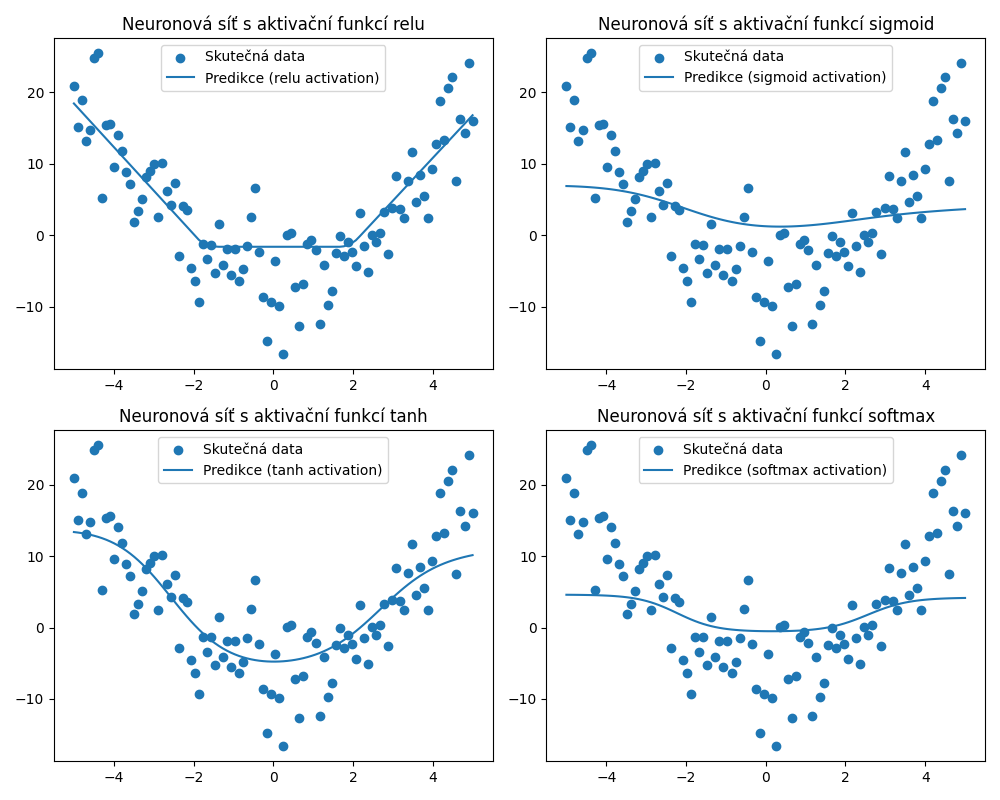
\includegraphics[width=1.0\textwidth]{obrazky-figures/nn_showcase.png}}
  \caption{Vliv aktivačních funkcí na klasifikaci}
  \end{center}\label{chart:activation_nn}
\end{figure}

\begin{itemize}
    \item \textbf{ReLU (Rectified Linear Unit)}: Nejčastěji používaná aktivační funkce ve skrytých vrstvách neuronových sítí kvůli své efektivitě a jednoduchosti. Její matematický popis je následující:
    \begin{equation}
        f(x) = \max(0, x)
    \end{equation}
    Tato funkce umožňuje modelu rychle konvergovat a snižuje pravděpodobnost gradientní degradace při dlouhém tréninku.
    
    \item \textbf{Sigmoid}: Funkce sigmoid je tradiční volba pro výstupní vrstvy binární klasifikace, protože její výstupy jsou omezeny na interval (0,1). Matematický popis funkce je:
    \begin{equation}
        f(x) = \frac{1}{1 + e^{-x}}
    \end{equation}
    Výstupy této funkce lze interpretovat jako pravděpodobnost.

    \item \textbf{Tanh (Hyperbolický Tangens)}: Funkce tanh je podobná sigmoidální funkci, ale její výstupy jsou normalizovány na rozsah (-1,1), což může vést k~rychlejší konvergenci během tréninku. Matematický popis:
    \begin{equation}
        f(x) = \tanh(x)
    \end{equation}
    Tato normalizace může vést k~lepšímu škálování gradientů.
    
    \item \textbf{Softmax}: Funkce softmax je rozšíření sigmoidní funkce pro více tříd a je často používána v~poslední vrstvě neuronových sítí pro více-třídní klasifikaci. Matematický popis funkce je:
    \begin{equation}
        \text{Softmax}(\mathbf{z})_i = \frac{e^{z_i}}{\sum_{j=1}^{K} e^{z_j}}
    \end{equation}
    kde \( \mathbf{z} \) představuje vstupní vektor a \( K~\) je počet tříd. Tato funkce vypočítává pravděpodobnosti tříd tak, že exponentně normalizuje výstupy vrstvy.
\end{itemize}


Výběr správné aktivační funkce závisí na specifickém úkolu a distribuci dat. Jak je vidět na obrázku \ref{chart:activation_nn}, různé aktivační funkce mohou vést k~odlišným výsledkům i pro stejná vstupní data, což zdůrazňuje jejich význam při návrhu architektury neuronové sítě.

\subsection{Architektura neuronových sítí}
Architektura neuronové sítě odkazuje na způsob, jakým jsou její komponenty uspořádány a propojeny. Tato část se zaměřuje na:

\begin{itemize}
    \item \textbf{Struktura a design:} Způsoby, jakými lze neurony a vrstvy organizovat pro různé typy úloh.
    \item \textbf{Výběr a nastavení vrstev:} Rozhodování o~počtu a typech vrstev pro specifické aplikace.
    \item \textbf{Konvoluční neuronové sítě (CNN):} Specifika a aplikace CNN, zvláště v~oblasti zpracování obrazu a vizuálního rozpoznávání.
    \item \textbf{Rekurentní neuronové sítě (RNN):} Význam a využití RNN v~kontextech, kde jsou důležité časové sekvence a vzory.
\end{itemize}






\subsection{Použití a vhodnost různých architektur neuronových sítí}
Výběr vhodné architektury neuronové sítě je zásadní pro úspěšnou detekci maligních domén. Konvoluční neuronové sítě (CNN) jsou obzvláště užitečné v~případech, kdy je potřeba extrahovat a identifikovat vzory z~vizuálních dat, díky své schopnosti efektivně zpracovávat a klasifikovat obrazy \cite{ml_general}. Na druhou stranu, rekurentní neuronové sítě (RNN) a jejich varianty, jako je LSTM (Long Short-Term Memory), jsou vhodnější pro úlohy, kde je důležitá časová posloupnost dat, jako je analýza časových řad nebo přirozeného jazyka \cite{9095044}.  V~kontextu detekce maligních domén může být kombinace obou těchto typů architektur efektivní, například použití CNN pro identifikaci vizuálních vzorců v~rámci webových stránek a RNN pro analýzu sekvenčního chování uživatelů nebo komunikace serverů. Další variantou rekurentních neuronových sítí jsou Gated Recurrent Units (GRU), které poskytují efektivní a méně výpočetně náročnou alternativu k~LSTM. GRU dokáží zachytit  dlouhodobé závislosti v~sekvenčních datech, což je klíčové pro detekci změn a anomálií v~doménových vzorcích. Díky své jednodušší struktuře a schopnosti minimalizovat problém degratujícího gradientu jsou GRU často preferovány v~případech, kdy je nutné rychle a efektivně zpracovávat velké objemy dat\cite{cho2014gru}. 

Níže \ref{chart:cnn_rnn} se nachází demonstrace rozdílu vstupních dat pro rekurentní a konvoluční neuronové sítě



\begin{figure}[h!]
  \begin{center}
   \raisebox{3.0mm}{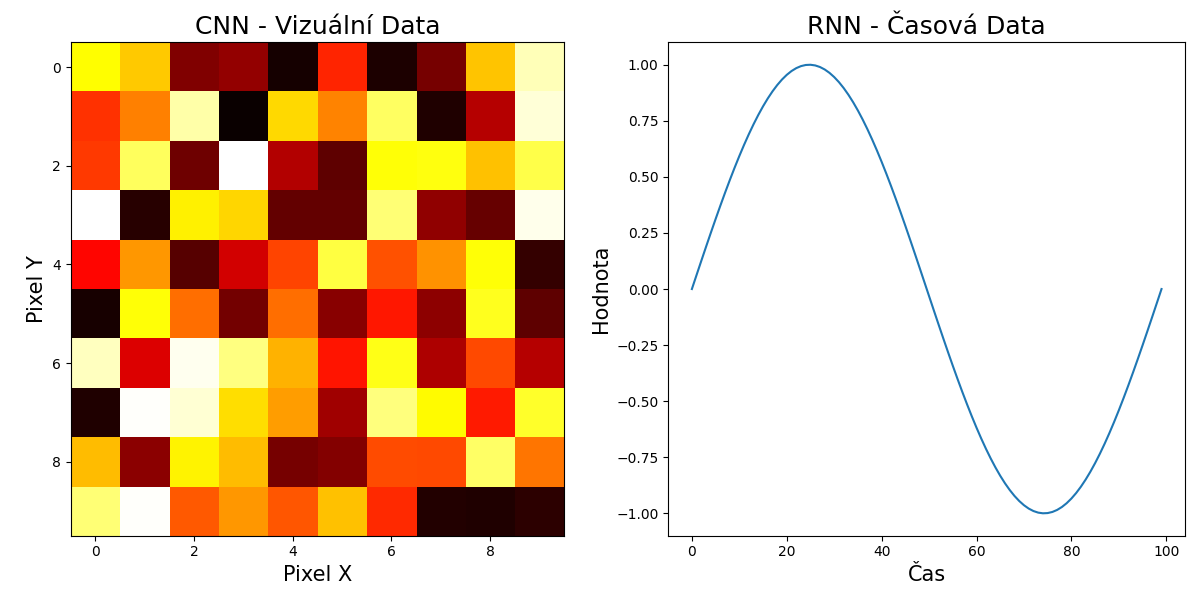
\includegraphics[width=1.0\textwidth]{obrazky-figures/nn_usecase.png}}
  \caption{Srovnání CNN a RNN}
  \end{center}\label{chart:cnn_rnn}
\end{figure}


\subsection{CNN}
Konvoluční neuronové sítě (CNN) představují významný pokrok v~oblasti strojového učení, zejména pro úkoly zpracování obrazových dat. Jejich schopnost efektivně identifikovat a klasifikovat vzory v~datech je zvláště užitečná při analýze dat domén, která často obsahují složité a bohaté informace s~obrazovými charakteristikami. Podobně jako v~obrazové analýze, kde CNN efektivně detekují a klasifikují různé vizuální prvky, mohou být tyto sítě aplikovány na data domén, aby rozpoznávaly specifické vzory a charakteristiky, které jsou indikativní pro určité kategorie domén. Díky schopnosti zpracovávat velké množství dat a extrahovat z~nich klíčové vlastnosti, jsou CNN ideálním nástrojem pro překlenutí komplexity a rozmanitosti v~datech domén \cite{cnn_data}.

Gated Recurrent Units (GRU) jsou efektivní variantou rekurentních neuronových sítí, která kombinuje jednoduchost a schopnost zachytit dlouhodobé závislosti v~sekvenčních datech. Oproti LSTM sítím využívají méně parametrů, což snižuje výpočetní náročnost, a přitom zachovávají vysokou schopnost učení. GRU byly představeny jako zjednodušená alternativa k~LSTM a ukázaly srovnatelný výkon při nižší složitosti modelu \cite{cho2014gru}.

Tato architektura se ukazuje jako vhodná pro analýzu sekvenčních dat doménových jmen, kde může efektivně identifikovat vzorce, jako jsou neobvyklé kombinace znaků nebo chování generované automaticky (např. DGA domény) \cite{cnn_gru_attention}.

Struktura GRU sítě typicky zahrnuje:
\begin{itemize}
    \item \textbf{Aktualizační a resetovací brány:} Umožňují efektivně řídit tok informací a eliminovat problém zmizelého gradientu.
    \item \textbf{Flexibilita:} Schopnost zachytit jak krátkodobé, tak dlouhodobé závislosti v~datech.
    \item \textbf{Nižší výpočetní náročnost:} Menší počet parametrů oproti LSTM umožňuje rychlejší trénink na velkých datových sadách.
\end{itemize}

\subsection{LSTM}

Long Short-Term Memory (LSTM) sítě, speciální typ rekurentních neuronových sítí, jsou zvláště vhodné pro lexikální analýzu doménových jmen z~několika důvodů. Prvním klíčovým aspektem je jejich schopnost zachytit dlouhodobé závislosti v~sekvenčních datech. V~kontextu doménových jmen může LSTM efektivně identifikovat a učit se ze vzorců v~sekvencích znaků, což je zásadní pro rozpoznávání anomálií nebo neobvyklých struktur, které často indikují škodlivé aktivity \cite{hochreiter1997lstm}.

Dále LSTM minimalizuje problém zmizelého gradientu, který je běžný u~tradičních RNN, díky své unikátní struktuře s~bránami pro zapomínání, vstup a výstup. Tato struktura umožňuje efektivnější trénink a lepší generalizaci při analýze složitých nebo zakódovaných jmen domén, kde je potřeba rozlišit legitimní domény od těch maligních. LSTM tak nabízí robustní rámec pro analýzu lexikálních charakteristik doménových jmen, což je klíčové pro včasnou a přesnou detekci potenciálně škodlivých webových aktivit \cite{cnn_gru_attention}.








\section{Metoda podpůrných vektorů (SVM)}

Metoda podpůrných vektorů, neboli \textit{Support Vector Machines} (SVM), je klasifikační algoritmus z~třídy algoritmů učení s~učitelem. SVM bylo původně vyvinuto jako pomocná metoda pro trénování neuronových sítí, ale později se ukázalo jako velmi efektivní samostatná klasifikační metoda \cite{cortes1995support}. Algoritmus je obzvlášť výhodný při práci s~daty o~vysoké dimenzi, a to zejména díky schopnosti najít optimální rozhodovací hranici mezi třídami \cite{GuyonElisseeff2003}.

Základním principem SVM je identifikace hyperroviny, která maximálně separuje klasifikované třídy a zároveň mezi nimi udržuje co největší možnou marginu. Pokud nejsou data lineárně separovatelná v~dané dimenzi, SVM využívá tzv. kernelovou transformaci – mapuje vstupní prostor do vyšší dimenze, kde separace možná je \cite{kernel_types}. Z~matematického hlediska lze téměř vždy najít vyšší dimenzi, ve které budou data separovatelná.

Klasifikátor SVM se sestává z~několika klíčových parametrů, které výrazně ovlivňují jeho chování i výsledky klasifikace:
\begin{itemize}
    \item Regularizační parametr \textbf{C}
    \item Jádrová funkce \textbf{kernel} a stupeň \textbf{degree}
    \item Koeficient \textbf{gamma}
\end{itemize}

\subsubsection{Regularizační parametr C}

Cílem algoritmu SVM je nalezení co nejrobustnější separace tříd. Parametr \textbf{C} představuje kompromis mezi maximalizací okraje a minimalizací chyb klasifikace. Nízké hodnoty \textbf{C} vedou k~větší toleranci pro chybně klasifikované vzory – model více generalizuje a je robustnější vůči šumu. Naopak vysoké hodnoty \textbf{C} kladou důraz na správnou klasifikaci trénovacích dat, což může vést k~přeučení (overfitting) \cite{cortes1995support, kernel_types}.


\begin{figure}[h!]
  \begin{center}
   \raisebox{3.0mm}{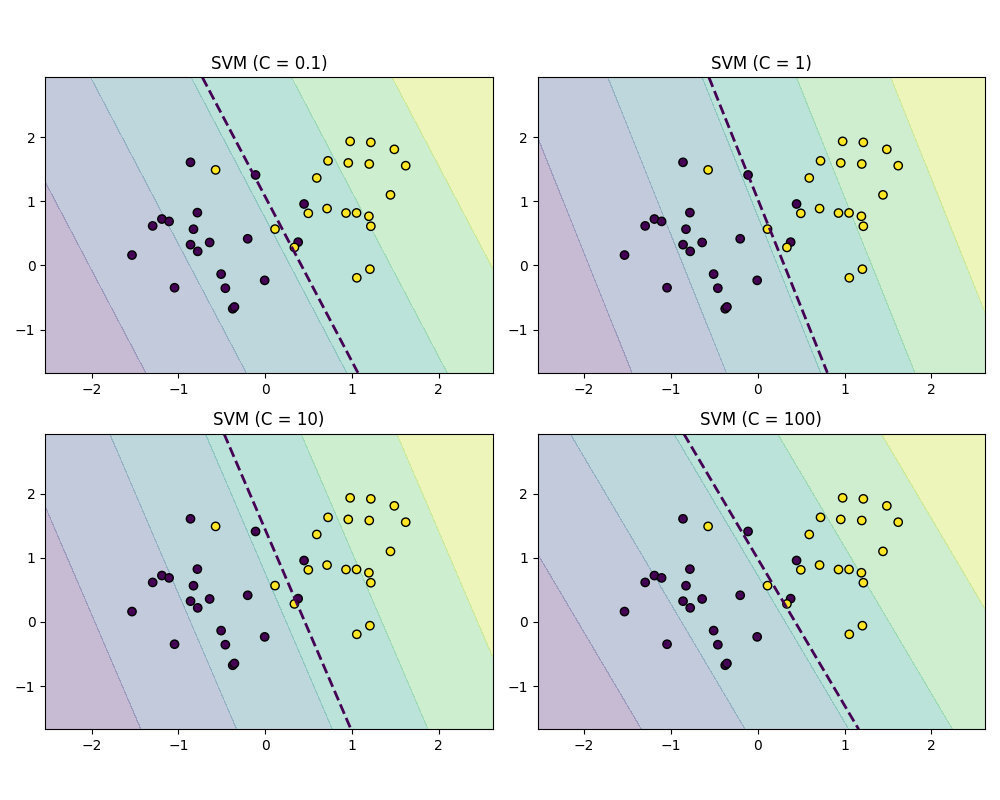
\includegraphics[width=1.0\textwidth]{obrazky-figures/SVM_C.png}}
  \caption{Vliv koeficientu \textbf{C} na klasifikaci SVM}
  \end{center}\label{chart:svm_c}
\end{figure}

V~grafu \ref{chart:svm_c} je demonstrován vliv změny tohoto parametru. V~případě vysokého koeficientu se metoda snaží zahrnout všechny body a tedy zvýšit přesnost klasifikace, ovšem na úkor schopnosti generalizovat. Opačný případ nastává pro malé hodnoty C. 

\subsubsection{Separující hyperrovina - kernel}
Pomocí tohoto parametru je možné volit matematický charakter hyperroviny, pomocí které jsou data separována a tedy klasifikována. Tato funkce může být lineárního i nelineárního charakteru. Vizualizace vlivu jádrové funkce je ilustrována na obrázku: \ref{chart:svm_kernel} \cite{kernel_types}. 


Nejpoužívanější funkce jsou pak: 
\begin{itemize}
    \item lineární 
    \item polynomiální
    \item rbf
    \item sigmoid
\end{itemize}


\begin{figure}[h!]
  \begin{center}
   \raisebox{3.0mm}{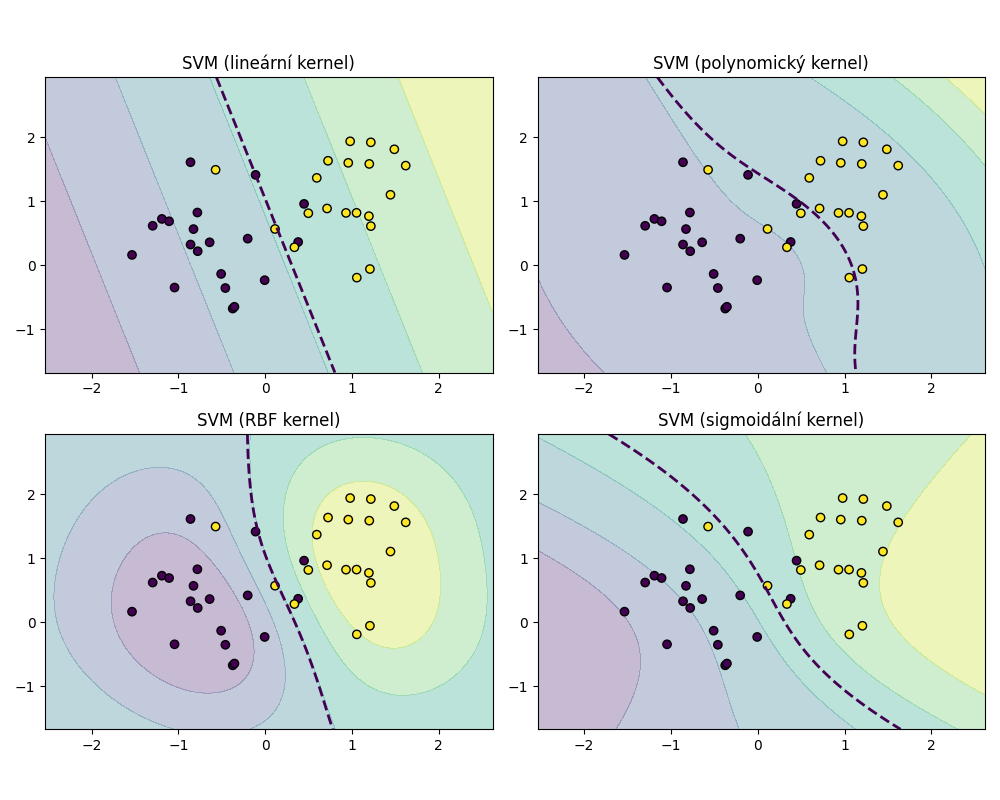
\includegraphics[width=1.0\textwidth]{obrazky-figures/svm_kernel_types.png}}
  \caption{Vliv výběru jádrové funkce na klasifikaci SVM}
  \end{center}\label{chart:svm_kernel}
\end{figure}


\subsubsection{Koeficient \textit{gamma}}

Koeficient gamma (\(\gamma\)) hraje klíčovou roli v~rámci klasifikace pomocí Support Vector Machines (SVM), zejména při použití Gaussiánského (RBF) jádra. Tento parametr určuje míru vlivu jednotlivých trénovacích vzorů na rozhodovací hranici. Čím vyšší je hodnota \(\gamma\), tím užší je oblast vlivu jednotlivých vzorů, což vede k~tvorbě složitějších, zakřivených hranic \cite{kernel_types}.

Zvýšením hodnoty \(\gamma\) dochází k~tomu, že model lépe zachytí lokální vlastnosti dat, což může zlepšit klasifikaci složitých struktur, ale zároveň zvyšuje riziko přetrénování (overfitting). Přetrénovaný model má tendenci přizpůsobit se šumu v~datech a selhává při generalizaci na neviděná data. Naopak nižší hodnoty \(\gamma\) vedou k~hladší a jednodušší rozhodovací hranici, což zvyšuje schopnost modelu generalizovat, avšak může vést k~nedostatečné přesnosti \cite{bergstra2011algorithms}.

Optimální hodnota parametru \(\gamma\) se zpravidla hledá pomocí technik, jako je křížová validace nebo bayesovská optimalizace hyperparametrů. Výběr správné hodnoty závisí na distribuci dat a složitosti klasifikační úlohy \cite{kernel_types, bergstra2011algorithms}.


\begin{figure}[h!]
  \begin{center}
   \raisebox{3.0mm}{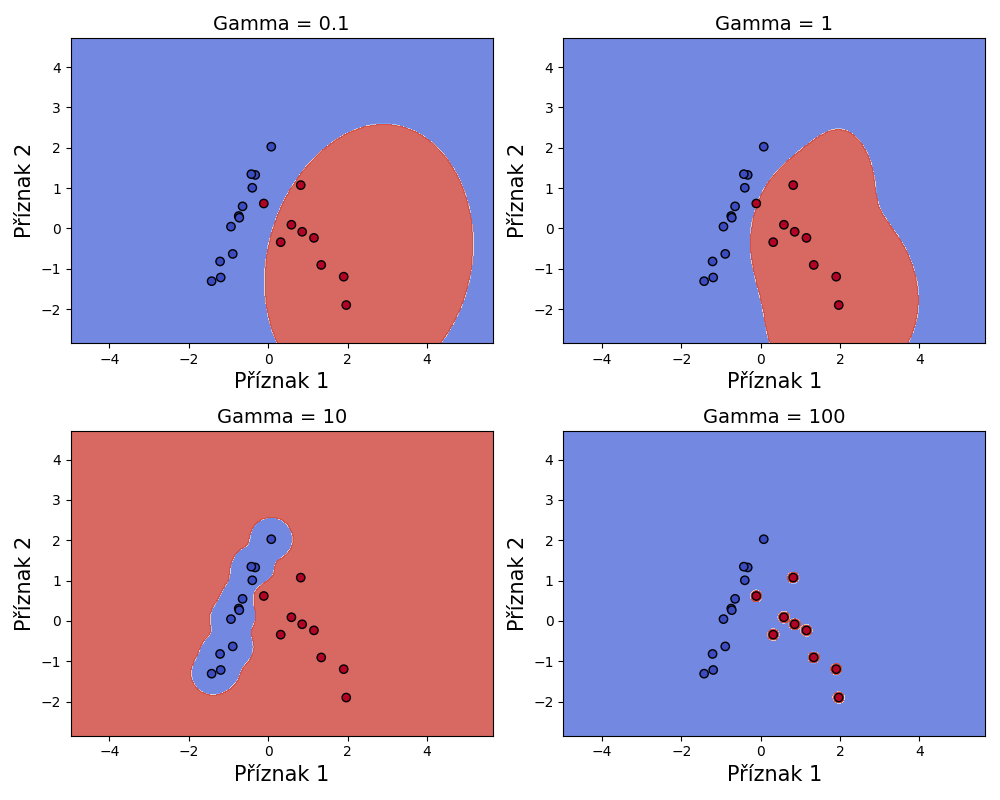
\includegraphics[width=0.9\textwidth]{obrazky-figures/svm_gamma_cz.png}}
  \caption{Vliv koeficientu \(\gamma\) na klasifikaci SVM}
  \end{center}\label{chart:gamma}
\end{figure}

\begin{itemize}
\item \textbf{Gamma = 0.1:} Na obrázku \ref{chart:gamma} je patrný větší vliv okolních bodů na tvar rozhodovací plochy. Model je méně přizpůsoben trénovacím datům a má tendenci k~jednoduššímu modelu.
\item \textbf{Gamma = 1:} S~hodnotou gamma rovno 1 (obrázek \ref{chart:gamma}) máme vyvážený přístup, kde vliv trénovacích bodů není příliš vysoký ani příliš nízký. Model je schopen efektivně generalizovat.

\item \textbf{Gamma = 10:} Zvýšení hodnoty gamma na 10 (obrázek \ref{chart:gamma}) vede k~tomu, že rozhodovací plocha je silně ovlivněna trénovacími body v~jejich bezprostředním okolí. Model se tím stává citlivějším na detaily dat.

\item \textbf{Gamma = 100:} Pro velmi vysokou hodnotu gamma (obrázek \ref{chart:gamma}) má rozhodovací plocha tendenci procházet jednotlivými trénovacími body, což může vést k~přeučení modelu na trénovací data.
\end{itemize}

V~obecnosti platí, že volba optimální hodnoty gamma závisí na konkrétních datech a cílech modelu. Je vhodné provádět ladění hyperparametrů (tj. volbu hodnoty gamma) pomocí validačních dat a sledovat výslednou výkonnost modelu na testovacích datech.





\subsection{Klasifikace pomocí SVM}
Algoritmus SVM je široce využíván pro klasifikaci maligních domén, a to zejména díky své schopnosti efektivně pracovat s~daty vysoké dimenze \cite{cortes1995support}. Je obzvlášť vhodný pro úlohy, kde je potřeba nalézt nelineární rozhodovací hranice v~komplexních datových strukturách. Překážkou však může být neuniformita vstupních dat – tedy různorodost typů příznaků (např. kombinace číselných, kategoriálních či binárních atributů).




\subsubsection{GridSearch}

Pro nalezení optimálních parametrů metody SVM se běžně používá technika zvaná GridSearch, která systematicky prochází předdefinované kombinace parametrů modelu \cite{bergstra2011algorithms}. Typicky zahrnuje volbu typu jádra (kernel), regularizačního faktoru \(C\) a parametru \(\gamma\) u~RBF jádra. Pro každou kombinaci parametrů se pomocí křížové validace (cross-validation) vyhodnocuje výkon modelu, často podle metrik jako jsou přesnost, skóre F1 nebo AUC \cite{bergstra2011algorithms, ml_general}. Přestože je GridSearch výpočetně náročný, jeho použití je zásadní pro dosažení maximální výkonnosti modelu v~reálném prostředí.







\section{Stromové algoritmy}

Stromové algoritmy se vyznačují schopností reprezentovat a modelovat rozhodovací procesy pomocí hierarchické struktury stromu, která reflektuje logiku rozhodování. Tyto algoritmy mají výhodu v~interpretovatelnosti a snadné vizualizaci, což je zásadní pro pochopení mechanismů, jež vedou k~jejich klasifikačním rozhodnutím \cite{quinlan1986induction}. V~kontextu detekce maligních domén, kde rychlá a spolehlivá klasifikace může znamenat rozdíl mezi úspěšnou prevencí a bezpečnostním rizikem, je důležité zhodnotit, jak efektivně tyto algoritmy identifikují potenciálně nebezpečné online entity \cite{silveira2021detection, zou2019detecting}.

Dále budou detailněji představeny nejpoužívanější stromové algoritmy, jako jsou například rozhodovací stromy (Decision Trees), náhodné lesy (Random Forests) či gradient boosting algoritmy. Zaměření bude následovat na porovnání těchto algoritmů v~kontextu ostatních metod klasifikace a objektivní srovnání jejich účinnosti v~rámci konkrétního bezpečnostního kontextu \cite{breiman2001random, ovi, ke2017lightgbm}.

\subsection*{Rozhodovací stromy - Decision Trees}

Rozhodovací stromy patří mezi základní a široce používané klasifikační algoritmy, které pracují na principu rekurzivního dělení datového prostoru na základě hodnot atributů. Výsledkem je struktura ve tvaru stromu, kde každý uzel reprezentuje rozhodovací pravidlo a listy pak odpovídají výsledným třídám \cite{quinlan1986induction}.

Mezi hlavní přednosti patří jejich vysoká interpretovatelnost a schopnost pracovat s~kategoriálními i číselnými atributy. Dokáží modelovat nelineární vztahy a jejich rozhodovací pravidla jsou snadno sledovatelná. Na druhou stranu jsou náchylné k~přeučení, zejména pokud nejsou ořezávány nebo je množina trénovacích dat omezená \cite{james2013introduction}.


\subsection*{Náhodné lesy - Random Forests}
Náhodné lesy představují kombinovanou metodu (ensemble), která kombinuje více rozhodovacích stromů za účelem zvýšení přesnosti a robustnosti klasifikace. Každý strom je trénován na náhodném vzorku dat a náhodné podmnožině atributů, což podporuje diverzitu mezi jednotlivými stromy a snižuje přeučení \cite{breiman2001random}.

Hlavní výhodou je vyšší odolnost vůči šumu a schopnost pracovat i s~rozsáhlými a nečistými daty. Algoritmus také poskytuje měření důležitosti atributů. Nevýhodou je nižší interpretovatelnost výsledků ve srovnání s~jednotlivými stromy a vyšší výpočetní náročnost \cite{liaw2002classification}.


\subsection*{Algoritmy na bázi Gradient Boosting}
Gradient Boosting je výkonná kombinovaná (ensemble) metoda, která buduje finální model iterativním přidáváním stromů, přičemž každý nový strom se snaží minimalizovat chyby předchozího modelu. Patří sem známé implementace jako XGBoost, LightGBM nebo CatBoost \cite{friedman2001greedy, chen2016xgboost, ke2017lightgbm}.

Mezi výhody patří vysoká přesnost, schopnost pracovat s~nevyváženými třídami a efektivní zpracování i velkých datasetů. Modely založené na gradient boosting však obvykle vyžadují důkladné ladění hyperparametrů a jejich interpretace bývá složitější ve srovnání s~jednoduššími stromovými metodami.


\noindent Další část práce bude zaměřena na konkrétní příklady a aplikace těchto stromových algoritmů v~oblasti detekce maligních domén, bude poskytnut přehled o~jejich úspěšnosti a efektivitě v~reálných podmínkách. Budou také diskutovány jejich limitace a možné další využití \cite{silveira2021detection, zou2019detecting}.


\section{Složené klasifikátory}

Kombinování různých metod strojového učení, známé také jako \textit{ensemble learning}, poskytuje robustní řešení pro zvýšení přesnosti a spolehlivosti klasifikačních modelů. Složené klasifikátory využívají výhod různorodých prediktivních modelů tím, že integrují jejich předpovědi a přispívají k~vytvoření silnějšího a více generalizovaného konečného modelu \cite{dietterich2000ensemble, wolpert1992stacking}. Tento přístup může být obzvláště účinný v~případech, kde jednotlivé modely jsou silné na různých typech dat nebo aspektech úlohy klasifikace. V~oblasti kybernetické bezpečnosti jsou kombinované (ensemble) metody často využívány ke kombinaci výstupů různých klasifikátorů, jako jsou SVM, rozhodovací stromy nebo neuronové sítě, s~cílem zvýšit robustnost proti chybné detekci \cite{bai2015bayesian}.


\begin{figure}[h!]
  \begin{center}
   \raisebox{3.2mm}{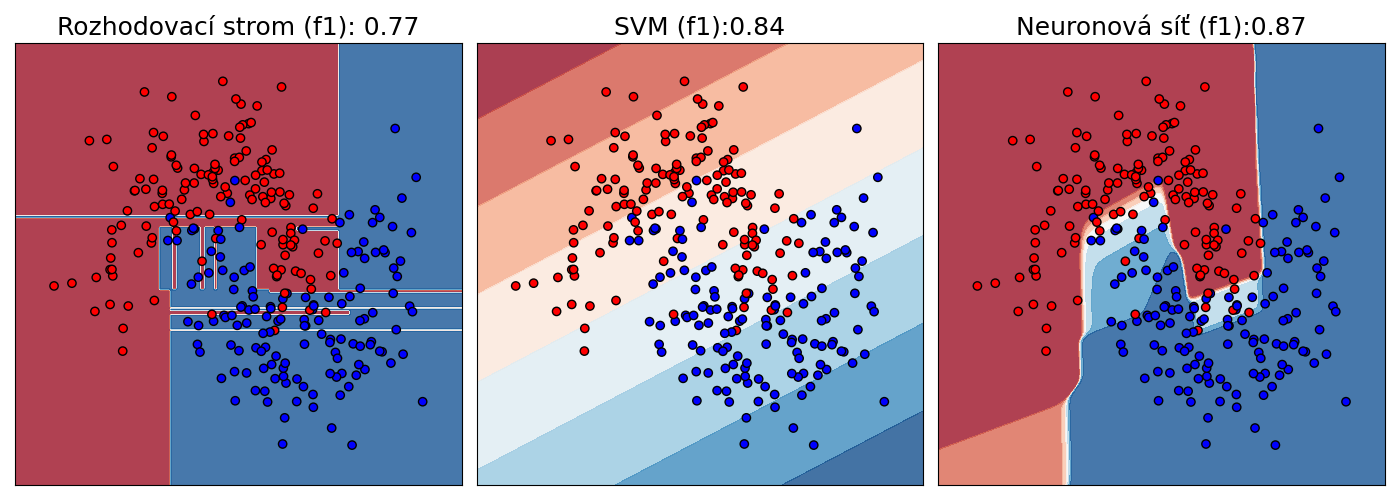
\includegraphics[width=1.0\textwidth]{obrazky-figures/weighted_nn_svm_tree.png}}
  \caption{Rozdíly klasifikačních metod}
  \end{center}\label{chart:weighted}
\end{figure}


Na obrázku \ref{chart:weighted} jsou zobrazeny rozhodovací hranice a skóre F1 pro tři různé klasifikační metody: rozhodovací strom, SVM a neuronovou síť. Rozhodovací strom, s~skóre F1 0.77, je schopen zachytit nelineární vzory v~datech, což je patrné z~komplexní struktury jeho rozhodovací hranice. Tato metoda je výhodná, pokud jsou data nelineárně separovatelná a obsahují rozhodovací pravidla, která mohou být reprezentována stromovými strukturami. Na druhé straně, SVM dosahuje skóre F1 0.84, což ukazuje na jeho schopnost efektivně najít optimální rozdělující hranici, zejména v~případě, že data jsou lineárně nebo téměř lineárně separovatelná. Nakonec neuronová síť, s~nejvyšším skóre F1 0.87, demonstruje svou schopnost vytvořit složité nelineární rozhodovací hranice díky použití aktivačních funkcí, což ji činí vhodnou pro složitější vzorce v~datech, které mohou být pro ostatní metody obtížně rozpoznatelné.


\subsection{Metody kombinování klasifikátorů}
Kombinování klasifikátorů je klíčovou strategií pro zvýšení přesnosti a spolehlivosti modelů strojového učení. Tato sekce detailně rozebírá tři hlavní přístupy: Bagging, Boosting a Stacking.

\subsubsection{Bagging}
Bagging (bootstrap aggregating) zvyšuje stabilitu a přesnost modelů tím, že kombinuje predikce více modelů, které byly trénovány na různých náhodných podmnožinách dat. Tento přístup snižuje variabilitu a zamezuje přeučení, což je zvláště užitečné pro modely citlivé na změny v~trénovacích datech, jako jsou rozhodovací stromy. Nejznámějším příkladem baggingu je Random Forest, který trénuje velké množství rozhodovacích stromů na různých vzorcích a kombinuje jejich výstupy prostřednictvím hlasování.

\textbf{Použití:} Bagging je ideální pro situace, kdy je cílem zvýšit robustnost modelů na šumových nebo nerovnoměrně rozložených datech. Například v~oblastech, jako je predikce zdravotních rizik nebo detekce anomálií, kde je stabilita modelu klíčová.

\textbf{Literatura:} Breiman, L. (2001). Random Forests. \textit{Machine Learning, 45}(1), 5–32. \cite{breiman2001random} Tato studie představuje Random Forest jako efektivní aplikaci baggingu, která přináší vysokou přesnost při zachování jednoduchosti.

\subsubsection{Boosting}
Boosting iterativně kombinuje slabé klasifikátory, jako jsou malé rozhodovací stromy, aby vytvořil silný model. Každý nový klasifikátor se zaměřuje na chyby předchozích modelů tím, že přiděluje vyšší váhy těm vzorkům, které byly klasifikovány nesprávně. Tím se postupně snižuje chyba modelu. AdaBoost a Gradient Boosting patří mezi nejčastěji používané algoritmy boostingu.

\textbf{Použití:} Boosting se často používá tam, kde je vyžadována vysoká přesnost a nízká míra chyb, například v~lékařské diagnostice nebo v~ekonomických predikcích. Je také oblíbený v~soutěžích v~oblasti strojového učení.

\textbf{Literatura:} Freund, Y., \& Schapire, R. E. (1997). A~decision-theoretic generalization of on-line learning and an application to boosting. \textit{Journal of Computer and System Sciences, 55}(1), 119–139. \cite{freund1997boosting} Tato práce představuje algoritmus AdaBoost jako základní metodu boostingu, která iterativně zlepšuje výkon modelu.

\subsubsection{Stacking}
Stacking kombinuje výstupy různých modelů prostřednictvím meta-modelu, který se učí optimálně kombinovat predikce jednotlivých základních modelů. Tento přístup umožňuje využít různé silné stránky jednotlivých modelů a zlepšit celkovou generalizaci.

\textbf{Použití:} Stacking je oblíbený při analýze komplexních dat, kde různé modely poskytují různé pohledy. Typickými oblastmi použití jsou predikce v~biologii, analýza trhu nebo zpracování přirozeného jazyka.

\textbf{Literatura:} Wolpert, D. H. (1992). Stacked generalization. \textit{Neural Networks, 5}(2), 241–259. \cite{wolpert1992stacking} Tento článek popisuje stacking jako metodu, která kombinuje různé klasifikátory pomocí meta-modelu, což výrazně zlepšuje přesnost a generalizaci.

\subsection{Vizualizace metod a efekt skládání}
Následující demonstrace zobrazuje rozdíl v~úspěšnosti klasifikace pomocí referenčních klasifikátorů a klasifikátorů vytvořených skládáním. 


Pro tuto demonstraci byla vygenerována datová sada 1000 2D bodů s~použitím python knihovny \textit{sklearn}. Jednotlivé příznaky jsou dále referencovány jako příznak 1 a 2.



\begin{figure}[h!]
    \centering
    \raisebox{3.2mm}{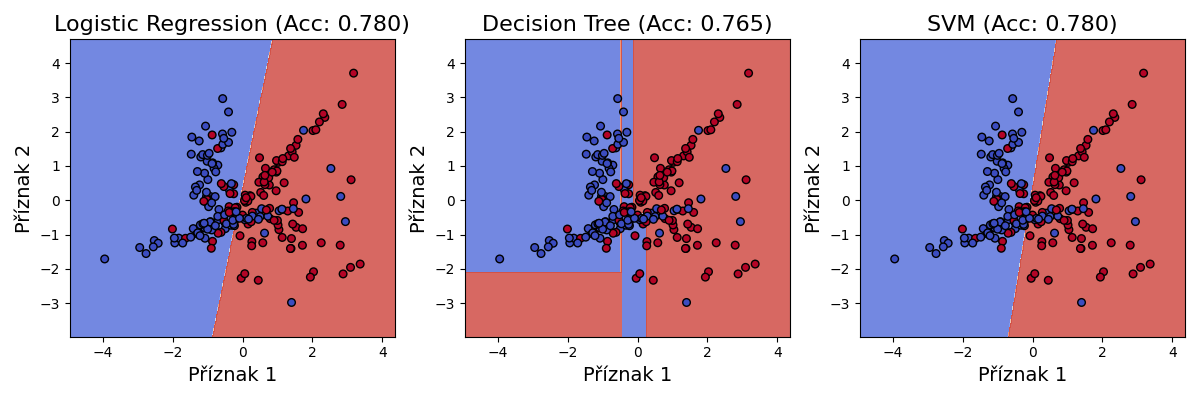
\includegraphics[width=1\textwidth]{obrazky-figures/before_sloz.png}}
    \caption{Klasifikace pomocí individuálních metod (LR, SVM, DT).}
    \label{fig:before_sloz}
\end{figure}

Obrázek \ref{fig:before_sloz} ukazuje rozhodovací hranice a přesnost základních modelů, které mohou být omezené při pokrývání komplexních nelineárních vzorů.

\begin{figure}[h!]
    \centering
    \raisebox{3.2mm}{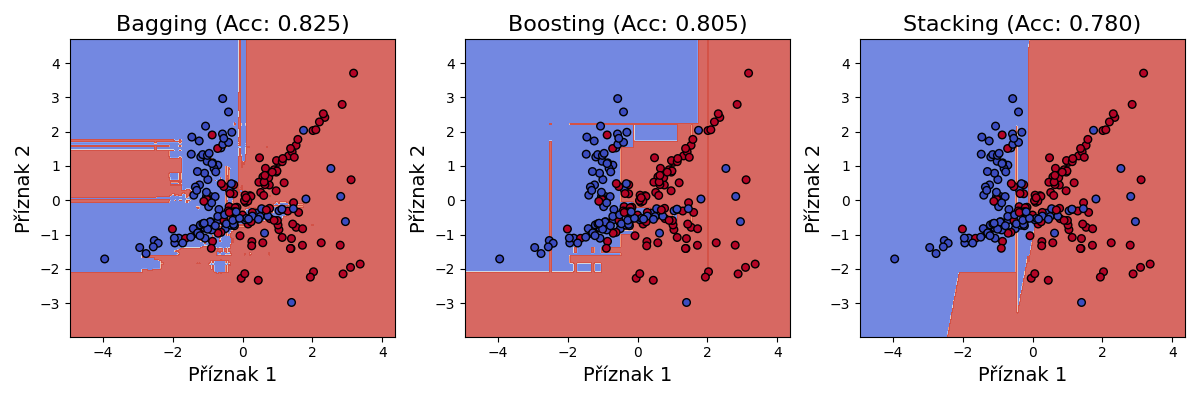
\includegraphics[width=1\textwidth]{obrazky-figures/after_sloz.png}}
    \caption{Klasifikace po aplikaci složených metod (Bagging, Boosting, Stacking).}
    \label{fig:after_sloz}
\end{figure}

Obrázek \ref{fig:after_sloz} zobrazuje zlepšení dosažené kombinací metod. Složené metody kompenzují chyby jednotlivých klasifikátorů a vytvářejí robustnější rozhodovací hranice, což vede ke zvýšení přesnosti.

Na základě analýzy metod kombinování klasifikátorů lze zobecnit jejich hlavní výhody a oblasti použití:

\begin{itemize}
    \item \textbf{Zvýšení přesnosti}: Kombinace predikcí různých modelů vede k~vyšší přesnosti, než kterou je schopný dosáhnout jednotlivý model samostatně. Tento efekt je způsoben tím, že různé modely zachytí různé aspekty dat, což je klíčové pro dosažení robustních výsledků \cite{nested_learning}.
    
    \item \textbf{Zlepšení generalizace}: Složené modely jsou schopny redukovat přeučení díky tomu, že chyby jednotlivých modelů se vzájemně kompenzují. Tato vlastnost zvyšuje schopnost modelů generalizovat na neviděných datech, což je zásadní zejména u~složitých úloh \cite{multi_stage_classification}.
    
    \item \textbf{Adaptabilita k~různým typům dat}: Díky kombinaci různorodých algoritmů dokáží složené klasifikátory lépe zvládat různé charakteristiky dat, například data s~šumem, komplexní nelineární vzory nebo nerovnoměrné rozdělení tříd \cite{fine_classification}.
\end{itemize}


\noindent Složené metody kombinování klasifikátorů tak představují efektivní nástroj pro řešení široké škály úloh strojového učení, od klasifikace po predikci a detekci anomálií.





\chapter{Datová sada a sběr}
\label{chapter:5}

Tato kapitola se věnuje původu datových sad a jejich následnému zpracování v~kontextu této diplomové práce. Je zde navázáno na výzkum projektu FETA. V~rámci této diplomové práce jsou navrženy dodatečné transformace a úprava formátu datových sad, pro efektivnější použití při trénování modelů strojového učení. První část se zaměřuje na popis charakteristiky a původu datových sad a ve druhé části jsou navrženy dodatečné metody zpracování a je zde demonstrován jejich přínos. 


\section{Datová sada}


V~rámci této diplomové práce byla využita datová sada, kterou jsem vytvořil společně se spoluautory článku připravovaného k~publikaci v~časopise \textit{Data in Brief} pod názvem \textit{A~Multi-Dimensional DNS Domain Intelligence Dataset for Cybersecurity Research}. Sada je ve formátu JSON a představuje export databáze z~MongoDB, kde jsou uchovávána data nasbíraná nástrojem \texttt{DomainRadar} \footnote{\url{https://github.com/nesfit/domainradar-dib}} \cite{domainradar}. Podrobnosti o~struktuře a obsahu dat jsou uvedeny v~detailu publikovaného datasetu na platformě \textit{Zenodo}: \footnote{\url{https://zenodo.org/records/13330073}}.



Datová sada obsahuje více než jeden milion domén, které jsou detailně anotovány jako benigní, phishingové nebo obsahující malware. Klíčovou vlastností této sady je její \textbf{multidimenzionální struktura}, která zahrnuje data z~následujících zdrojů:
\begin{itemize}
    \item \textbf{DNS záznamy:} Informace o~doménových jménech, jako jsou A, AAAA, MX nebo NS záznamy.
    \item \textbf{TLS certifikáty:} Detailní informace z~TLS handshake a certifikátů.
    \item \textbf{RDAP a WHOIS:} Metadata o~registraci domén.
    \item \textbf{Geolokační data:} Informace o~poloze IP adres získané z~databáze GeoLite2.
    \item \textbf{Reputační data:} Údaje o~doménách a IP adresách z~platformy VirusTotal a dalších zdrojů.
\end{itemize}
Datová sada je formátována ve formátu JSON, což usnadňuje její integraci do analytických nástrojů a využití ve strojovém učení.

\subsection{Deskriptivní statistiky datové sady}

Tabulka \ref{tab:dataset_summary} poskytuje přehled o~základní struktuře datové sady, včetně počtu domén v~jednotlivých kategoriích a zdrojů dat.

\begin{table}[h!]
\centering
\begin{tabular}{|l|c|c|}
\hline
\textbf{Kategorie} & \textbf{Počet domén} & \textbf{Zdroj} \\
\hline
Benigní (Cisco Umbrella) & 368,956 & Cisco Umbrella Top 1 Million \\
\hline
Benigní (CESNET) & 461,338 & akademická síť  CESNET \\
\hline
Phishingové & 164,425 & PhishTank, OpenPhish \\
\hline
Malware & 100,809 & ThreatFox, URLHaus, další černé listiny \\
\hline
\end{tabular}
\caption{Přehled jednotlivých kategorií a jejich zdrojů v~datové sadě.}
\label{tab:dataset_summary}
\end{table}


\subsubsection{Datová sada phishing domén}
Datová sada phishingových domén, sbíraná v~průběhu roku 2023 a 2024, představuje komplexní sadu dat určenou k~identifikaci phishingových útoků. Tato datová sada obsahuje následující charakteristiky:


Phishingové domény byly získány z~OpenPhish \cite{openphish-web}, automatizované platformy pro phishingovou inteligenci, a PhishTank \cite{phishtank-web}, kolaborativní databáze pro data a informace o~phishingu. Obě platformy důkladně ověřují hlášené domény, čímž snižují počet falešně pozitivních výsledků. Domény byly sbírány z~jejich MISP kanálů, jakmile byly publikovány. Sběr vyústil v~164,901 potenciálních phishingových domén. Další filtrování bylo provedeno prostřednictvím služby VirusTotal \cite{virtotal}, kterou provozuje Chronicle Security a která detekuje škodlivý obsah v~souborech a URL, včetně detekce podvodných phishingových stránek. Pomocí API VirusTotal bylo identifikováno a odstraněno 476 chybně klasifikovaných domén. Toto filtrování vyústilo ve vysoce kvalitní datovou sadu 164,425 ověřených phishingových domén. 


\subsubsection{Datová sada benigních domén}
K~získání sady benigních domén byl použit veřejně dostupný seznam Top One Million od platformy Cisco Umbrella \cite{cisco-umbrela-web}. 

Tento seznam byl dále zpracován a filtrován, aby bylo zajištěno, že obsahuje pouze benigní domény. Byl implementován proces filtrování inspirovaný metodologií Rahbarinia a kol.~\cite{rahbarinia2015segugio}. Tento přístup zahrnuje extrakci měsíčních dat, pro tento milion nejvyhledávanějších domén a provedení selekce takových domén, které se zde nacházejí pravidelně. Dodatečné benigní domény byly získány z~provozu v~akademických sítích. 


\subsubsection{Datová sada malware domén}

Domény obsahující malware byly získány ze služby ThreatFox, což je online platforma poskytující komplexní přehled a analýzy ohledně hrozeb spojených s~malware. ThreatFox se specializuje na shromažďování a poskytování podrobných informací o~doménách, IP adresách a hash hodnotách souborů spojených s~nejrůznějšími typy malware. Díky této službě je možné identifikovat aktuální a vznikající hrozby v~kyberprostoru \cite{threatfox-web}.

Domény byly průběžně sbírány v~průběhu roku 2023 a 2024, čímž bylo zajištěno, že datová sada reflektuje aktuální stav a dynamiku v~oblasti malware domén. Vzhledem k~tomu, že životnost malware domén není dlouhá a jejich charakteristiky se mohou rychle měnit, bylo nezbytné zajistit co nejrychlejší sběr a analýzu dat. Po sběru dat byly k~doménám ihned doplněny informace, které umožňují jejich efektivní klasifikaci a analýzu.

Pro validaci a odstranění chybně nahlášených domén bylo využito služby VirusTotal, která poskytuje rozsáhlou detekci škodlivého obsahu v~souborech a URL, včetně detekce phishingových a malware domén. Tento proces dalšího ověřování zvyšuje kvalitu a spolehlivost datové sady \cite{virtotal}.



\subsection{Verifikační datová sada}
\label{clftest}

Pro účely nezávislého ověření klasifikační výkonnosti modelů byla vytvořena separátní verifikační datová sada, která nebyla nijak využita při trénování ani ladění modelů. Tato sada slouží k~testování schopnosti modelu generalizovat na dosud neznámá data, pocházející z~odlišného časového období i zdrojů. 

Sběr dat probíhal ve dnech 23. až 25. května 2024. Benigní domény byly zachyceny z~běžného provozu na síti CESNET, což odpovídá autentickému provozu v~akademickém prostředí. Naopak škodlivé domény byly získány z~veřejně dostupných databází \textit{OpenPhish} \cite{openphish-web}, \textit{PhishTank} \cite{phishtank-web} a z~komunitně spravovaného blacklistu \textit{StevenBlack}, dostupného na platformě Github\footnote{\url{https://github.com/StevenBlack/hosts}}.

Celkový rozsah verifikační sady činil 5\,048 domén:
\begin{itemize}
    \item 4\,276 benigních domén
    \item 480 phishingových domén
    \item 292 malware domén
\end{itemize}

Stejně jako u~hlavní datové sady byly všechny škodlivé domény podrobeny kontrole prostřednictvím služby VirusTotal \cite{virtotal}, aby byla zajištěna jejich aktuálnost a validita. Podrobný popis této verifikační metodiky je uveden v~sekci \ref{filtering}.

Verifikační sada tak představuje nezávislý a realistický vzorek domén, umožňující objektivní měření robustnosti a reálné použitelnosti navržených klasifikačních přístupů.


\section{Zdroje dat}
Data domén z~výše uvedených datových sad byla získána z~různých zdrojů, zahrnující jak veřejně dostupné bezpečnostní feedy, tak i specializované databáze. Mezi hlavní zdroje dat patří: \cite{petr}
\begin{itemize}
    \item \textbf{VirusTotal}: Online platforma poskytující nástroje pro analýzu URL a souborů pomocí více antivirových nástrojů.
    \item \textbf{Bezpečnostní feedy a černé listiny}: Databáze obsahující seznamy známých maligních domén, jako je MISP a PhishTank.
    \item \textbf{RDAP a WHOIS databáze}: Informace o~registračních údajích domén. 
\end{itemize}



\section{Metodologie a proces sběru domén}
Filtrování dat bylo prováděno na základě několika klíčových kritérií, aby byla zajištěna kvalita a spolehlivost datových sad. Hlavní kroky zahrnovaly: \cite{petr}
\begin{itemize}
    \item \textbf{Validace doménových jmen}: Využití API VirusTotal k~ověření aktuálního stavu domén (maligní/benigní).
    \item \textbf{Čištění dat}: Odstranění duplicitních záznamů, neúplných dat a domén s~nespecifikovanými atributy.

\end{itemize}

\noindent Domény byly získány z~různorodých zdrojů a následně obohaceny o~doplňující informace prostřednictvím nástroje \textit{DomainRadar}, který vznikl v~rámci řešení projektu FETA. Na jeho vývoji jsem se podílel jako spoluautor. Tento nástroj využívá moduly implementované v~jazyce Python pro sběr dat z~externích služeb, jako jsou WHOIS/RDAP dotazy nebo extrakce TLS certifikátů.


\subsection{DomainRadar}
\label{domainradar}

V~rámci této diplomové práce byl zásadním nástrojem pro sběr a zpracování dat systém \textbf{DomainRadar} \cite{domainradar}, který vznikl na Fakultě informačních technologií VUT v~Brně jako součást projektu \textit{Metody AI pro zabezpečení kybernetického prostoru a řídicí systémy} (FIT-S-20-6293, 2020–2023). Jedná se o~komplexní, modulárně navržený systém pro aktivní i pasivní sběr, ukládání a analýzu doménových dat. Jeho cílem je efektivní příprava datových sad pro analýzu hrozeb, detekci škodlivých domén a vývoj modelů strojového učení. Systém je dostupný jako výzkumný prototyp \footnote{\url{https://www.fit.vut.cz/research/product/c179852/.en}}.

DomainRadar je tvořen sadou specializovaných kolektorů, které získávají informace o~doménách z~různých zdrojů — například DNS záznamy, RDAP metadata, TLS certifikáty, reputační informace, geolokaci IP adres nebo informace o~ASN. Jednotlivé datové proudy jsou následně zpracovávány pomocí komponent jako \textbf{Data Merger}, které sjednocují data do jednotného JSON formátu a ukládají je do databáze \textbf{MongoDB}. Architektura systému je založena na \textbf{Apache Kafka}, která slouží k~orchestraci sběru a oddělení jednotlivých fází pipeline. Jednotlivé komponenty systému jsou znázorněny na obrázku \ref{fig:domainradar_flow} v~sekci pojednávající o~procesu sběru. 

Získaná data jsou následně zpracovávána pomocí nástroje \textbf{Feature Extractor}, který převádí JSON reprezentaci domén na numerické vektory příznaků. Ty jsou ukládány ve formátu \textbf{Apache Parquet}\footnote{\url{https://parquet.apache.org/}}, a to ve dvou verzích: (1) jako surové cache výstupy z~databáze a (2) jako finální vektory příznaků připravené pro strojové učení. 



\subsubsection{Domain Collector}

Softwarem ze kterého vychází systém DomainRadar je systém \textbf{Domain Collector} \cite{fit-vut-product-784}, který umožňuje automatizovaný sběr, agregaci a ukládání informací o~doménách. Tento nástroj využívá data ze zdrojů jako \textbf{Cisco Umbrella}, \textbf{PhishTank}, \textbf{OpenPhish}, \textbf{ThreatFox} a dalších threat intelligence platforem. Získaná data jsou obohacena pomocí aktivního sběru (např. ICMP testy, TLS handshaky) a následně ukládána do MongoDB pro další zpracování.


\subsection{Segmentovaný proces sběru}
\label{subsection:colect}

\begin{figure}[!h]
    \centering
    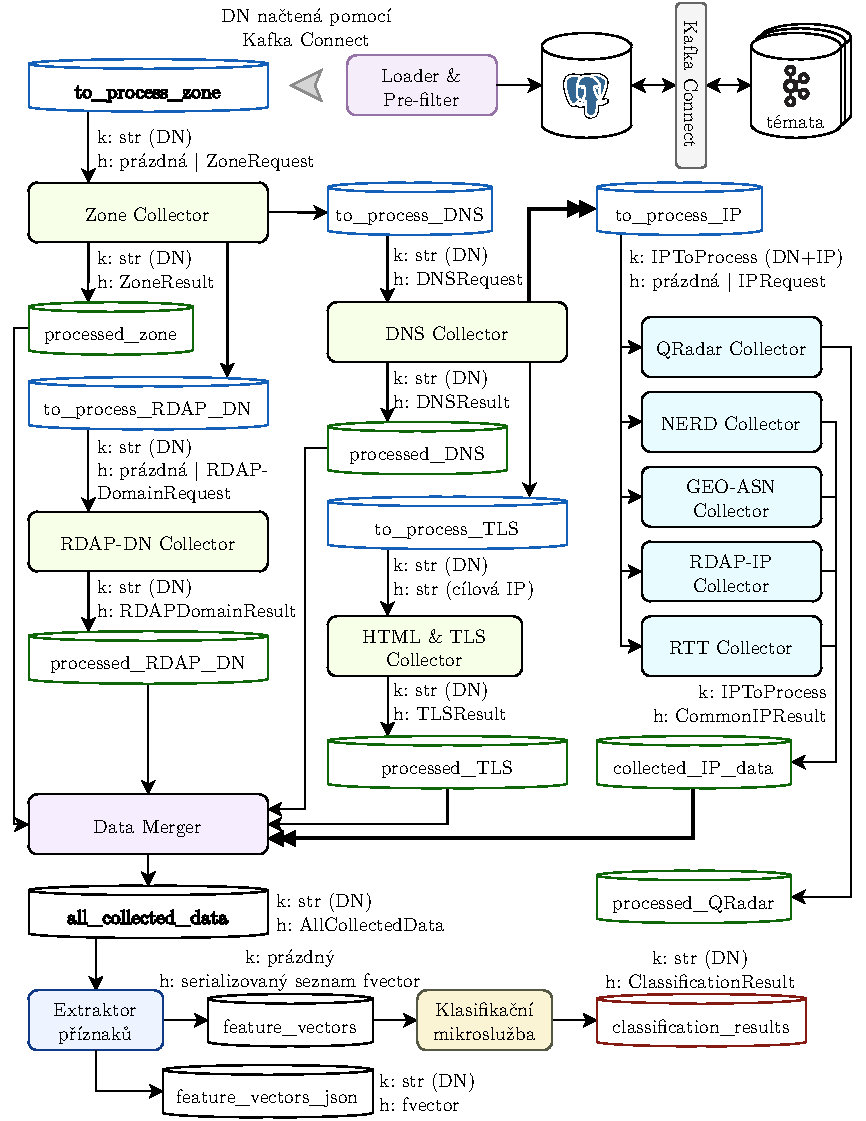
\includegraphics[width=1.0\textwidth]{obrazky-figures/domainradar_colector.pdf}
    \caption{Schéma segmentovaného procesu sběru dat v~systému DomainRadar \cite{domainradar}, převzato z~\cite{oondra}.}
    \label{fig:domainradar_flow}
\end{figure}

Schéma na obrázku~\ref{fig:domainradar_flow} znázorňuje komponenty systému \textbf{DomainRadar}, které zajišťují plně automatizovaný a hierarchicky uspořádaný sběr dat o~doménách. Celý proces je navržen jako sekvence na sebe navazujících kroků, kde každý z~kolektorů doplňuje doménový záznam o~specifický typ informací — od základních syntaktických rysů až po reputační skóre IP adres a metainformace z~TLS certifikátů.

Tato hierarchická struktura sběru má přímý dopad na návrh skupin příznaků a definici jejich logického rozšiřování. Strategie konstruování vektorů příznaků ve třech úrovních — od čistě lexikálních až po plně obohacené záznamy s~RDAP a HTML — přímo vychází z~architektury tohoto systému. Tato souvislost je blíže popsána v~sekci~\ref{logi_step}.

\paragraph{Načtení a filtrování domén.}

Na vstupu systému figuruje komponenta \textbf{Loader \& Pre-filter}, která načítá seznamy domén (např. z~PostgreSQL databáze) a prostřednictvím Kafka Connect je vkládá do tematických front. Tato komponenta zároveň filtruje již dříve zpracované domény, čímž zamezuje duplicitnímu sběru.

\paragraph{Sběr dat pomocí kolektorů.}

Domény postupně procházejí skrze sadu asynchronně volaných sběračů:

\begin{itemize}
    \item \textbf{Zone Collector} – získává základní informace z~TLD zón.
    \item \textbf{DNS Collector} – zajišťuje DNS záznamy (A, AAAA, MX, NS...).
    \item \textbf{RDAP-DN Collector} – provádí RDAP dotaz na registrátora domény.
    \item \textbf{HTML \& TLS Collector} – navazuje TLS spojení a získává informace o~certifikátu.
    \item \textbf{IP kolektory} – navazují na IP adresy získané z~DNS a doplňují:
    \begin{itemize}
        \item \textbf{QRadar Collector} – reputace IP z~bezpečnostních databází,
        \item \textbf{NERD Collector} – stav IP z~NERD databáze,
        \item \textbf{GEO-ASN Collector} – geografii a číslo AS,
        \item \textbf{RDAP-IP Collector} – RDAP údaje k~IP,
        \item \textbf{RTT Collector} – měření odezvy IP.
    \end{itemize}
\end{itemize}

\noindent Každý kolektor odesílá výstup do specifického tématu v~Kafce (např. \texttt{processed\_TLS}), odkud jsou data odeslána k~agregaci.

\paragraph{Agregace a extrakce příznaků.}

Všechny informace jsou sloučeny pomocí komponenty \textbf{Data Merger} do jednotné struktury \texttt{all\_collected\_data}. Tento výstup je předán do \textbf{extraktoru příznaků}, který data převede na číselné vektory. Ty jsou následně serializovány a uloženy ve formátu \textbf{Apache Parquet}.

Nástroj pro extrakci\footnote{\url{https://github.com/nesfit/domainradar-training/tree/main/feature-extraction}} podporuje jak export pro dávkové trénování, tak i klasifikaci v~reálném čase pomocí klasifikační mikroslužby.


\paragraph{Neúplnost záznamů.}

Vzhledem k~povaze sběru dat není garantováno, že pro každou doménu budou k~dispozici všechny typy dat. Například:

\begin{itemize}
    \item doména nemusí mít validní TLS endpoint,
    \item RDAP servery mohou být nedostupné,
    \item IP může chybět v~reputační databázi.
\end{itemize}

Tato neúplnost ovlivňuje dostupnost příznaků, a tím i konstrukci datových subsetů. Práce proto zohledňuje rozdílné úrovně datové úplnosti v~návrhu experimentů i hodnocení výsledků (viz sekce~\ref{subsection:agg_res}).

Pipeline systému DomainRadar je navržena s~důrazem na modularitu a možnost připojení dalších zdrojů dat, včetně paralelního zpracování rozsáhlých datových sad.


\section{Verifikace Ground-truth} \label{pravda}
Ground-truth (česky "referenční pravda") představuje v~kontextu strojového učení a datové analýzy označení pro data, jejichž správná klasifikace je známa a ověřena. V~rámci této práce ground-truth kolekce reprezentují doménová jména, u~kterých bylo na základě víceúrovňové verifikace potvrzeno, zda se jedná o~domény benigní, phishingové nebo sloužící k~šíření malwaru. Tato referenční data jsou zásadní pro správné trénování a hodnocení klasifikačních modelů, protože určují správné cílové hodnoty, vůči kterým jsou měřeny chyby modelu. K~ověření pravdivosti datových sad byla implementována následující strategie: \cite{petr}

\begin{itemize}
    \item Všechny domény byly analyzovány pomocí akademické verze VirusTotal API, která poskytuje víceúrovňové hodnocení pomocí různých antivirových enginů.
    \item Výsledky analýz byly zpracovány pomocí skriptu pro hromadné označování domén jako maligních nebo benigních.
    \item Finální verifikace byla provedena porovnáním s~veřejně dostupnými seznamy černých listin a ručním přezkoumáním podezřelých vzorků.
\end{itemize}
Tento přístup zajistil, že vytvořená datová sada obsahuje kvalitní a spolehlivá data, která slouží jako základ pro trénování a testování klasifikačních modelů \cite{petr}.


\section{Filtrování datových sad}
\label{filtering}

Aby bylo možné zaručit vysokou kvalitu a spolehlivost vytvořených datových sad, bylo nezbytné aplikovat systematický proces filtrování doménových záznamů. Tento proces přímo navazuje na segmentovanou architekturu systému \textbf{DomainRadar}, jejíž výstupem je kolekce domén uložená v~databázi \textbf{MongoDB} a následně exportovaná ve formátu \textbf{Apache Parquet}\footnote{\url{https://parquet.apache.org/}}.

Důvodem volby právě tohoto formátu je jeho přímá návaznost na výstupní fázi sběrové pipeline (viz sekce~\ref{subsection:colect}). V~systému DomainRadar vznikají typicky dva druhy Parquet souborů:

\begin{itemize}
    \item \textbf{Raw Parquet} – dočasný výstup generovaný z~MongoDB projekcí, obsahující původní JSON data získaná kolektory (DNS, RDAP, TLS, atd.),
    \item \textbf{Parquet feature vektory} – zpracovaná reprezentace vytvořená nástrojem \textit{Feature Extractor}, kde jsou jednotlivé domény reprezentovány jako číselné vektory připravené pro klasifikaci.
\end{itemize}

Použitý extraktor je veřejně dostupný v~repozitáři \footnote{\url{https://github.com/nesfit/domainradar-training/tree/main/feature-extraction}} systému DomainRadar.

Filtrování bylo aplikováno buď přímo nad těmito Parquet soubory, nebo ve specifických případech nad extrahovanými seznamy domén. Další sekce pak popisují konkrétní mechanismy filtrace.


\subsection{Ověřování domén pomocí VirusTotal}

Pro externí ověření důvěryhodnosti domén byla použita služba \textbf{VirusTotal}, která kombinuje detekční výsledky desítek antivirových enginů a reputačních databází. Systém načetl domény ze vstupního Parquet souboru, odeslal je pomocí oficiálního API ke kontrole a následně extrahoval metriky jako \textit{detection count}, \textit{malicious flag} a seznam identifikovaných detekcí.

Jak ukazuje obrázek~\ref{fig:vt_interaction}, celý proces ověřování byl automatizován a navázán na další filtrovací mechanismy. Na základě výstupů z~VirusTotal byly domény rozděleny do kategorií (např. spolehlivě benigní, podezřelé, potvrzené škodlivé) a pouze validované domény byly zařazeny do finální datové sady.

\begin{figure}[H]
    \centering
    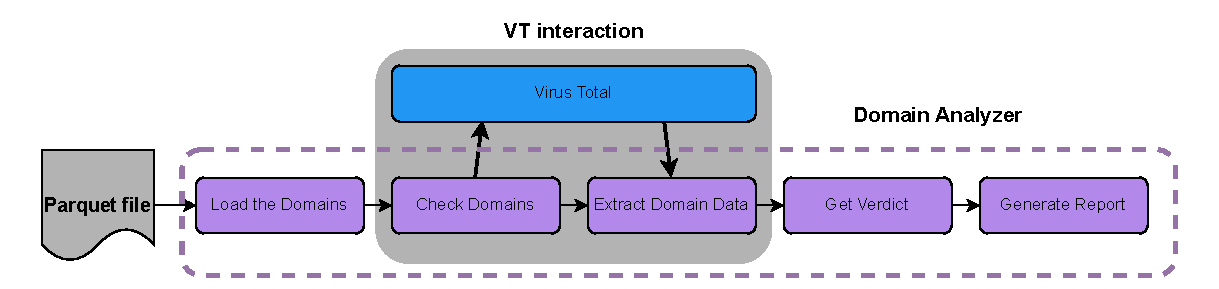
\includegraphics[width=1.0\textwidth]{obrazky-figures/vt.pdf}
    \caption{Interakce se službou VirusTotal v~rámci ověřování domén. Převzato z~dokumentace systému DomainRadar \cite{domainradar}.}
    \label{fig:vt_interaction}
\end{figure}

\subsection{Filtrace domén z~dat ze sítě CESNET}

Specifickým případem byl sběr benigních domén z~akademické sítě CESNET. Tyto domény byly považovány za potenciálně důvěryhodné, ale bylo nezbytné odstranit technické domény, překlepy a domény s~příliš nízkým výskytem.

Aplikován byl dvoustupňový filtrační proces, který kombinuje:

\begin{enumerate}
    \item \textbf{Intersekci na základě výskytu} – ponechány byly pouze domény, které se vyskytovaly v~provozu pravidelně a opakovaně.
    \item \textbf{Suffix redukci} – odstraněny byly domény, které měly společný kořen nebo generické TLD bez informativní hodnoty (např. \texttt{cdn}, \texttt{akamaiedge}).
    \item \textbf{Podvzorkování} – pro zajištění vyváženosti mezi třídami byly některé domény náhodně vybrány, aby odpovídaly velikostně ostatním kategoriím.
\end{enumerate}

Celý proces je znázorněn na obrázku~\ref{fig:cesnet_filtering}, který je převzat z~práce P. Pouče \cite{petr}.

\begin{figure}[H]
    \centering
    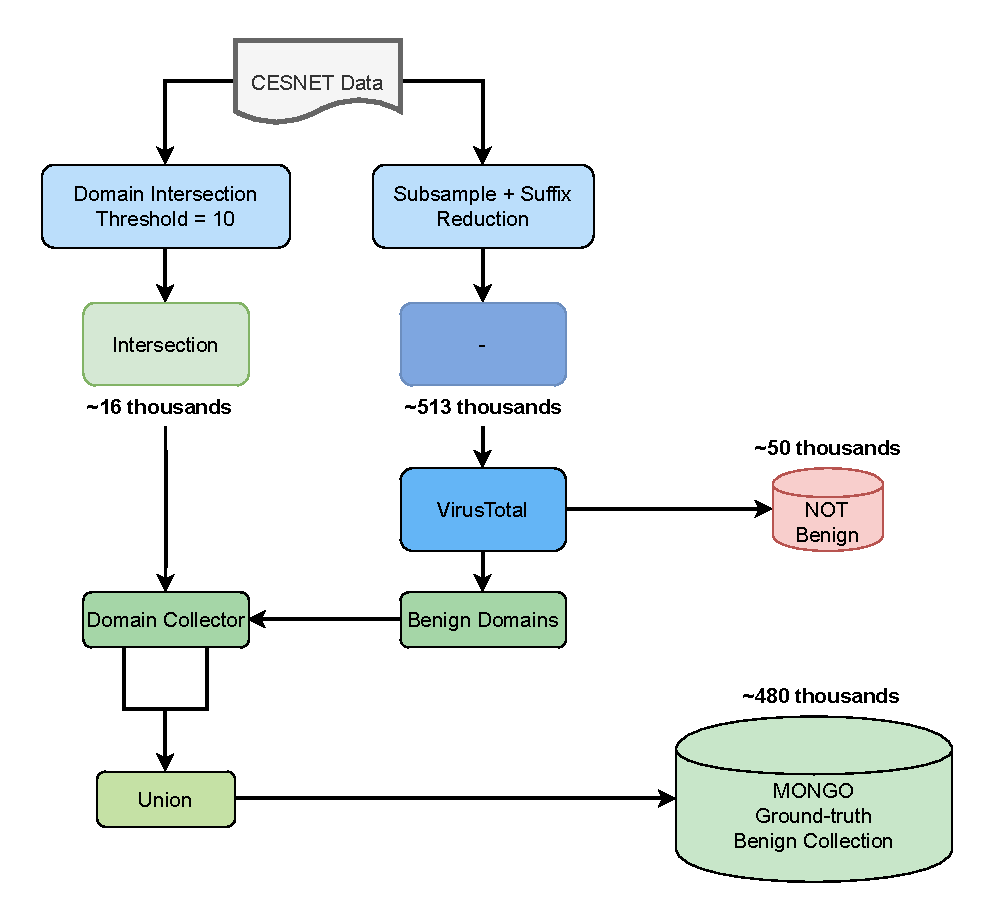
\includegraphics[width=0.9\textwidth]{obrazky-figures/cesnet-filtering.pdf}
    \caption{Proces filtrace domén získaných z~CESNET dat. Převzato z~práce P. Pouče \cite{petr}.}
    \label{fig:cesnet_filtering}
\end{figure}

\subsection{Shrnutí}

Použitím kombinace vícestupňového filtrování, validace třetí stranou (VirusTotal) a heuristik vyvinutých pro akademický provoz byly vytvořeny vysoce kvalitní datové sady s~minimem chybné klasifikace. Tento proces navazuje na architekturu sběru dat systému DomainRadar a jeho výstupní Parquet formát, čímž je zajištěna konzistence celého pipeline od sběru až po klasifikaci.


\section{Transformace datových příznaků}
\label{data-transform}

Pro účely efektivního trénování klasifikátorů bylo nezbytné navrhnout systematický postup předzpracování doménových dat. Vstupní data byla dodána ve formě \texttt{parquet} souborů obsahujících nezpracované příznaky domén (např. počty záznamů, délku názvu, entropii, geolokační informace apod.). Aby bylo možné tyto příznaky použít pro strojové učení, bylo nutné provést několik kroků transformace, které lze rozdělit na dvě hlavní fáze: \textbf{obecné předzpracování}, které je shodné pro všechny modely a \textbf{modelově specifické transformace}, odrážející potřeby individuálních modelů. 

\subsection{Obecné předzpracování}
\label{general_transformation}
Tato fáze byla společná pro všechny klasifikační modely a aplikovala se na celou datovou množinu.

\begin{enumerate}
    \item \textbf{Čištění a typová normalizace:} Chybějící hodnoty byly nahrazeny nulami, binární příznaky převedeny na celočíselné reprezentace (0/1), a redundantní nebo nekonzistentní sloupce byly odstraněny.
    
    \item \textbf{Min-max škálování:} Všechny příznaky byly převedeny do jednotného rozsahu $[0, 1]$ pomocí standardního min-max škálování:
    \begin{equation}
        x_{ij}^{\text{scaled}} = \frac{x_{ij} - \min_j}{\max_j - \min_j}
    \end{equation}
    kde $x_{ij}$ je původní hodnota příznaku $j$ pro vzorek $i$.

    \item \textbf{Odstranění odlehlých hodnot:} Pro zvýšení robustnosti modelů byly odstraněny extrémní hodnoty na základě jejich vzdálenosti od průměru. Hodnota byla považována za odlehlou, pokud:
    \begin{equation}
        x < \mu - 2\sigma \quad \text{nebo} \quad x > \mu + 2\sigma
    \end{equation}
    kde $\mu$ je průměr a $\sigma$ směrodatná odchylka daného příznaku.

\end{enumerate}

Tento obecný postup zajišťuje, že všechny vstupní atributy jsou srovnatelné a vhodné pro většinu algoritmů strojového učení, zejména těch, které jsou citlivé na měřítko (např. SVM nebo kNN).

\subsection{Modelově specifické transformace}
Některé modely vyžadují dodatečné transformace vstupních dat, které reflektují jejich interní fungování. Typickým příkladem jsou neuronové sítě, které těží z~hladce rozložených vstupů v~omezeném rozsahu.

\subsubsection*{Sigmoidní transformace}
\label{sigmoid_transformation}
U~neuronových sítí byla po základním škálování aplikována navíc sigmoidní funkce, která převede hodnoty do intervalu $(0, 1)$ a zároveň zvýrazní rozdíly v~okolí nulové hodnoty:

\begin{equation}
    x_{ij}^{\text{sigmoid}} = \frac{1}{1 + e^{-(a_{ij} - \mu_j)/\sigma_j}}
\end{equation}

Zde $a_{ij}$ představuje škálovanou hodnotu příznaku, $\mu_j$ a $\sigma_j$ odpovídají průměru a směrodatné odchylce daného příznaku. Tato transformace pomáhá stabilizovat zpětnou propagaci chyb a zmírňuje výskyt problémů jako \textit{exploding} nebo \textit{vanishing gradients}.


\subsubsection*{2D transformace dat domén}
\label{2d_transformation}

Pro účely konvoluční neuronové sítě (CNN) je nezbytné transformovat doménová data do dvourozměrného (2D) formátu. Tato transformace umožňuje využití technik z~oblasti zpracování obrazu, jako je detekce vzorů prostřednictvím konvolučních vrstev. V~našem případě jsou jednotlivé atributy dat škálovány do intervalu [0, 1], což umožňuje interpretovat je jako intenzity pixelů. 

Vizualizace na obrázku \ref{image:cnn} demonstruje, jak je každá doména reprezentována jako 2D snímek, kde každý pixel odpovídá jednomu atributu. Proces transformace dat je založen na převodu jednorozměrného vektoru atributů na dvourozměrný obraz. Nechť $n$ je počet atributů (prvků) v~každém vzorku, pak strana čtverce $s$ pro reprezentaci dat ve 2D prostoru je dána výrazem:

\[
s~= \lceil \sqrt{n} \rceil,
\]

kde $\lceil \cdot \rceil$ označuje zaokrouhlení nahoru. Tímto způsobem je každý vektor atributů o~velikosti $n$ transformován na matici o~rozměrech $s \times s$. Tento postup je aplikován na všechny vzorky v~trénovací i testovací sadě dat. Takto přetransformovaná data jsou vhodná pro zpracování pomocí CNN, což umožňuje efektivní detekci a klasifikaci vzorů a charakteristik v~datech.


\begin{figure}[h!]
  \begin{center}
   \raisebox{3.2mm}{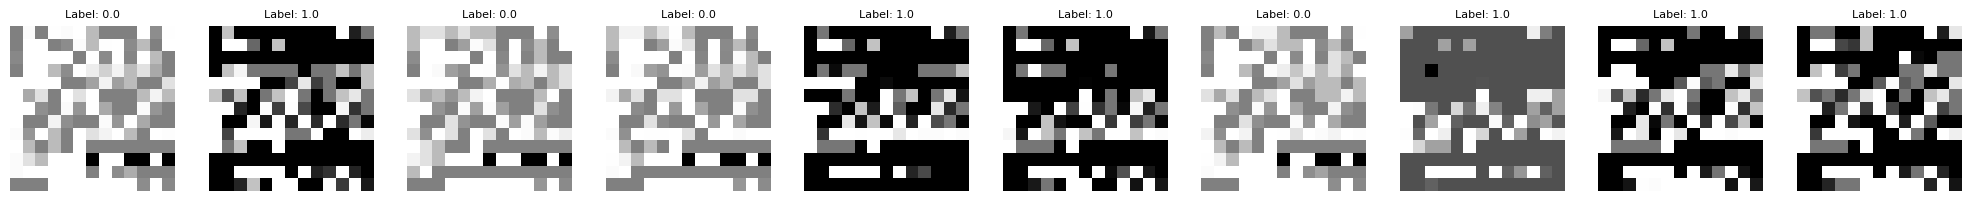
\includegraphics[width=1.0\textwidth]{obrazky-figures/visualized_cnn.png}}
  \caption{Vizualizace domén předpřipravených pro CNN}
  \end{center}\label{image:cnn}
\end{figure}



\subsection{Vizualizace a dopad transformací}

Na obrázku~\ref{fig:features1} je ukázáno srovnání mezi nezpracovanou a zpracovanou verzí příznaku \texttt{dns\_NS\_count}. Je patrné, že odstraněním odlehlých hodnot a následným škálováním došlo k~výraznému zlepšení rozložení hodnot, což je žádoucí pro zajištění konzistentního trénování modelů.

\begin{figure}[h!]
    \centering
    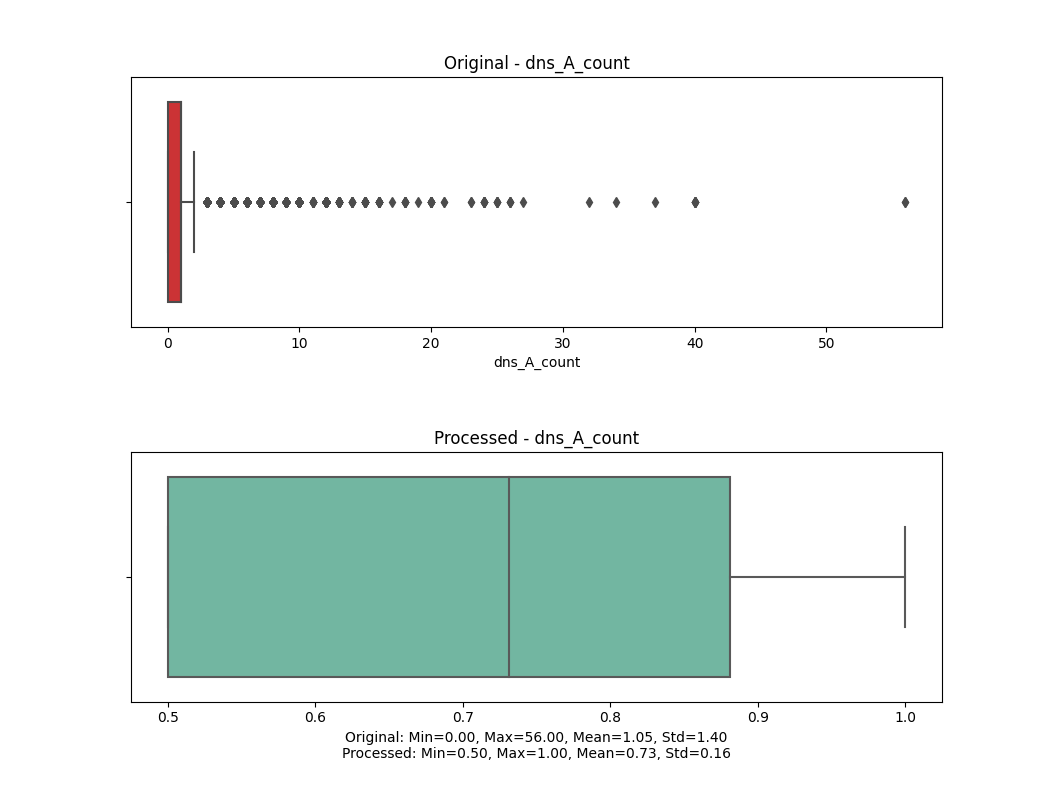
\includegraphics[width=1.0\textwidth]{obrazky-figures/features_1.png}
    \caption{Porovnání zpracovaných a nezpracovaných hodnot příznaku \texttt{dns\_NS\_count}.}
    \label{fig:features1}
\end{figure}

Transformace dat tímto způsobem zajišťuje, že výsledné atributy jsou numericky stabilní, vhodné pro strojové učení a zároveň robustní vůči šumu a extrémům v~datech. Na jednotlivé modely se v~dalších kapitolách odkazujeme vždy s~poznámkou, jaké konkrétní části tohoto postupu byly využity.



% Schema jak bych mel mit tuhle sekci 
% 6.0 Úvod +kategorie 
%     - Krátký úvod 
%     - Popis kategorií příznaků, názvosloví
% 6.1 srovnání 
% 6.2 metodologie
% domainradar fíčury
% 6.3 vlastní fíčury 

\chapter{Tvorba a segmentace  příznaků}
\label{chapter:6}
Úspěšná detekce phishingových a malwarových domén je podmíněna vhodnou
reprezentací vstupních dat, tedy takovou sadou příznaků, která co
nejlépe zachycuje rozdíly mezi benigními a škodlivými doménami.

Tato kapitola proto nejprve vymezuje \textbf{terminologii}
a zpřesňuje kategorie příznaků, z~nichž je sestaven vektor použitý ve
všech následných experimentech. Následně jsou prezentována
\textbf{vlastní měření a srovnání současných přístupů} popsaných v~literatuře a je diskutován jejich praktický dopad na klasifikační úspěšnost.
Třetí část formuluje \textbf{metodologii tvorby příznaků} vycházející
z~nástroje \texttt{DomainRadar} a definuje subsety různé náročnosti
sběru. \cite{fit-vut-product-838}  Kapitola je zakončena cíleným \textbf{feature engineeringem pro
TLS certifikáty}, jenž rozšiřuje původní vektor o~atributy s~vysokým
diskriminačním potenciálem.

Veškeré analýzy a výsledné metriky vycházejí z~datové sady
popsané v~kapitole~\hyperref[chapter:5]{5}.


\section{Terminologie a kategorie příznaků}

Základem této práce je vektor příznaků převzatý z~nástroje \mbox{\texttt{DomainRadar}}, který obsahuje celkem \textbf{263} atributů. 
Tabulkový přehled všech použitých příznaků je uveden v~příloze~\ref{app:feature_vector}~\cite{domainradar}.
Příznaky byly vytvořeny v~rámci publikace~\cite{noms} a vývojového produktu~\cite{fit-vut-product-838}, na nichž jsem se podílel jako spoluautor.


\noindent Všechny atributy byly rozděleny podle původu do následujících
kategorických skupin:

\begin{itemize}
  \item \textbf{LEX} – lexikální příznaky odvozené přímo
        z~doménového jména; zahrnují délku druhé úrovně,
        Shannonovu entropii, četnosti znaků či \textit{n}-gramové
        shody.
  \item \textbf{DNS} – parametry DNS odpovědí, například počty
        jednotlivých RR typů, průměrné hodnoty TTL
        nebo skóre DNSSEC.
  \item \textbf{IP} – charakteristiky IP adres navázaných na doménu
        (počet IPv4/IPv6, diverzita autonomních systémů,
        rozptyl RTT).
  \item \textbf{TLS} – vlastnosti TLS handshake a certifikátů,
        např. verze protokolu, použitá cipher-suite,
        délka a validita certifikačního řetězce.
  \item \textbf{GEO} – geolokační údaje IP adres získané
        z~databází MaxMind GeoLite2 (země, region,
        vzdálenost k~měřícímu uzlu).
  \item \textbf{RDAP/WHOIS} – informace o~registraci a vlastnictví
        domény, stáří, registrátor či využití anonymizačních služeb.
  \item \textbf{HTML} – atributy odvozené z~obsahu webové stránky,
        jako je počet rámců či přítomnost formulářů.
  \item \textbf{MISC} – doplňkové příznaky, jež nelze jednoznačně
        zařadit (např.~TLD abuse score).
\end{itemize}
\label{item:segment}

\noindent Kromě uvedených základních kategorií byly zkoumány také různé \emph{agregace} těchto skupin, přičemž byl brán ohled na obtížnost a časovou náročnost sběru jednotlivých atributů vycházející z~technické implementace nástroje DomainRadar \cite{domainradar}.


\section{Srovnání existujících příznaků}
\label{sec:feature-survey}

V~rámci tohoto výzkumu byly replikovány přístupy vybraných studií uvedených v~kapitole~\ref{chapter:2}.  
Z~původních článků byla vždy převzata definice příznaků a implementován odpovídající transformační skript, který vytvořil vektorové reprezentace potřebné pro trénink klasifikačních modelů.  
Pro každý zdrojový článek byl použit klasifikátor doporučený autory; v~případech neúplné specifikace hyperparametrů byly tyto nalezeny metodou \emph{grid-search}.  
Pokud studie nabízela více algoritmů, byl do tabulky zařazen ten s~nejvyšší dosaženou hodnotou~F1.

Tabulka~\ref{tab:method_comparison_intext} shrnuje nejlepší replikované výsledky na vlastní datové sadě z~kapitoly~\ref{chapter:5}.  
Hodnoty tedy neodpovídají číslům převzatým z~originálních publikací, nýbrž skóre naměřenému v~jednotném prostředí tohoto výzkumu.  
Tyto výsledky následně sloužily jako východisko pro návrh vlastních rozšíření popsaných v~navazujících kapitolách.


\begin{table}[H]
  \centering
      \begin{tabular}{@{}lcccccc@{}}
        \toprule
        \textbf{První autor} & \textbf{Rok} & \textbf{Typ} &
        \textbf{Nejlepší F1} & \textbf{\# f.} &
        \textbf{Kat.\ přízn.} & \textbf{Model}\\
        \midrule
        Torroledo   & 2018 & Malw   & 0.966 & 30 & TLS           & LightGBM\\
        Shi         & 2017 & Mix    & 0.915 &  9 & MIX           & LightGBM\\
        Magalhães   & 2020 & Mix    & 0.969 & 17 & MIX           & LightGBM\\
        Zhu         & 2019 & Mix    & 0.910 & 11 & MIX           & AdaBoost\\
        Kumar       & 2022 & Malw   & 0.932 & 15 & LEX           & AdaBoost\\
        Silveira    & 2021 & Mix    & 0.921 & 19 & DNS           & SVM\\
        Iwahana     & 2021 & Mix    & 0.968 & 25 & MIX           & LightGBM\\
        Gopinath    & 2020 & C\&C   & 0.937 & 17 & WHOIS+DNS     & LightGBM\\
        Hason       & 2020 & Mix    & 0.971 &  9 & MIX           & LightGBM\\
        Chatterjee  & 2019 & Phish  & 0.924 & 14 & MIX           & XGBoost\\
        Sadique     & 2020 & Phish  & 0.924 & 20 & MIX           & XGBoost\\
        \bottomrule
      \end{tabular}
    \caption{Replikace vybraných studií}
    \label{tab:method_comparison_intext}
\end{table}



\subsubsection{Nejpoužívanější příznaky}

Na základě analýzy tabulky \ref{tab:method_comparison_intext} můžeme identifikovat nejčastěji používané typy příznaků a jejich variabilitu mezi jednotlivými přístupy. Nejčastěji se objevují kombinované příznaky (MIX), které zahrnují různé aspekty doménových charakteristik, jako jsou DNS záznamy, TLS certifikáty nebo lexikální rysy doménových jmen. Tento přístup je patrný zejména ve studiích autorů Shi kol. \cite{Shit}, Iwahana kol. \cite{max2020madmax} a Hason kol. \cite{hason2020robust}, kteří dosahují průměrných skóre F1 mezi 0.90 a 0.95. Kombinované příznaky poskytují vyváženou reprezentaci dat a umožňují klasifikátorům efektivněji generalizovat.

Dalším často používaným typem příznaků jsou příznaky založené na TLS certifikátech, jak ukazuje práce Torroleda a kol.~\cite{torroledo2018hunting}, která dosahuje velmi vysokého skóre F1 (0{,}9245). TLS příznaky jsou klíčové zejména v~kontextu bezpečnostních atributů a spolehlivosti domén. Tento přístup těží z~hluboké analýzy certifikátů a jejich atributů, jako jsou délka platnosti, certifikační autorita nebo typ validace. V~příloze~\ref{appendix:tls-results} této práce je uveden experimentální klasifikátor založený výhradně na TLS příznacích, který byl navržen s~cílem ověřit jejich samostatnou výpovědní hodnotu. Ačkoliv jeho výkon nedosahuje úrovně kombinovaných modelů, výsledky naznačují, že TLS certifikáty mohou poskytovat doplňkový signál užitečný zejména v~případech, kdy jiné datové zdroje nejsou dostupné.


Naopak méně časté jsou příznaky založené výhradně na lexikální analýze (LEX), jak ukazuje studie Kumar \cite{kumar}, která i přes menší množství příznaků (15) dosahuje skóre F1 0.87. Lexikální příznaky se zaměřují na strukturu a vzorce v~doménových jménech, což může být užitečné zejména pro detekci domén generovaných algoritmy (DGA). Jejich omezené rozšíření může souviset s~tím, že samy o~sobě neposkytují kontextuální ani síťové informace.

Příznaky založené na DNS a WHOIS záznamech se objevují méně často, ale stále hrají důležitou roli. Například studie Gopinatha \cite{gopinath2020whois} ukazuje, že kombinace těchto příznaků může vést k~solidním výsledkům s~skóre F1 0.87. Tyto příznaky zahrnují informace o~registraci domény, geografii serverů a metriky DNS dotazů, které pomáhají identifikovat nově registrované nebo podezřele krátkodobě aktivní domény.





\section{Metodologie tvorby příznaků} \label{sec:feature-engineering-methodology}

V~návaznosti na výsledky replikovaných studií a vlastní analýzy byl navržen systematický postup tvorby a rozšiřování příznaků, s~cílem maximalizovat klasifikační úspěšnost při detekci phishingových a škodlivých domén.

Výchozí inspirací pro metodologii byl nástroj \texttt{DomainRadar}, jenž byl rozšířen na základě poznatků získaných v~rámci výzkumu publikovaného v~\cite{CNSM}. Tento přístup kombinuje více zdrojů dat (DNS, RDAP, TLS, IP, GEO) a vytváří komplexní vektor popisující doménu.

Na základě analýzy Shapleyho hodnot (SHAP) bylo ověřeno, že všechny hlavní kategorie příznaků přispívají k~rozhodovacímu procesu, avšak jejich přínos není rovnoměrný. Největší význam vykazovaly atributy odvozené z~\textbf{RDAP} (registrace domén a IP), následované \textbf{DNS} a \textbf{lexikálními} vlastnostmi. Oproti očekávání se ukázalo, že \textbf{TLS} příznaky mají výrazně menší dopad na rozhodování klasifikátorů, s~výjimkou několika specifických parametrů, jako je vyjednaná šifra nebo délka certifikačního řetězce.

\subsection{Agregovaná analýza přínosu kategorií}

Na základě výsledků dřívější analýzy publikované v~článku \textit{Spotting the Hook}~\cite{CNSM} byla provedena agregovaná interpretace významu jednotlivých kategorií příznaků pomocí Shapleyho hodnot vypočtených nad modelem LightGBM. Výpočty vycházejí z~předchozí podmnožiny datové sady, která neobsahovala data z~CESNETu a obsahovala menší zastoupení phishingových a malware domén.

Jak ukazuje obrázek~\ref{fig:aggregated-shap}, nejvyšší přínos k~rozhodování vykazuje skupina RDAP příznaků, následovaná IP, LEX a GEO atributy. Naopak DNS a TLS příznaky měly ve srovnání s~ostatními kategoriemi menší význam.


\begin{itemize}
    \item \textbf{RDAP} – Nejvýznamnější skupina, zejména atributy jako věk domény a vlastnosti registrátora.
    \item \textbf{IP} – Entropie IP prefixů, počet autonomních systémů a další příznaky odvozené z~dat IP adres přispívaly k~odhalení phishingu.
    \item \textbf{LEX} – Vysoký význam měly zejména skóre zneužití TLD a \textit{n}-gramové shody.
    \item \textbf{GEO} – Střední přínos; geografické rozložení serverů pomáhalo diferencovat legitimní a podvodné domény.
    \item \textbf{DNS} – Nízké TTL hodnoty a charakteristiky rekordů se ukázaly jako užitečné.
    \item \textbf{TLS} – Nejmenší agregovaný vliv, s~výjimkou vybraných atributů (vyjednaná šifra, délka řetězce certifikátů).
\end{itemize}

\begin{figure}[h]
    \centering
    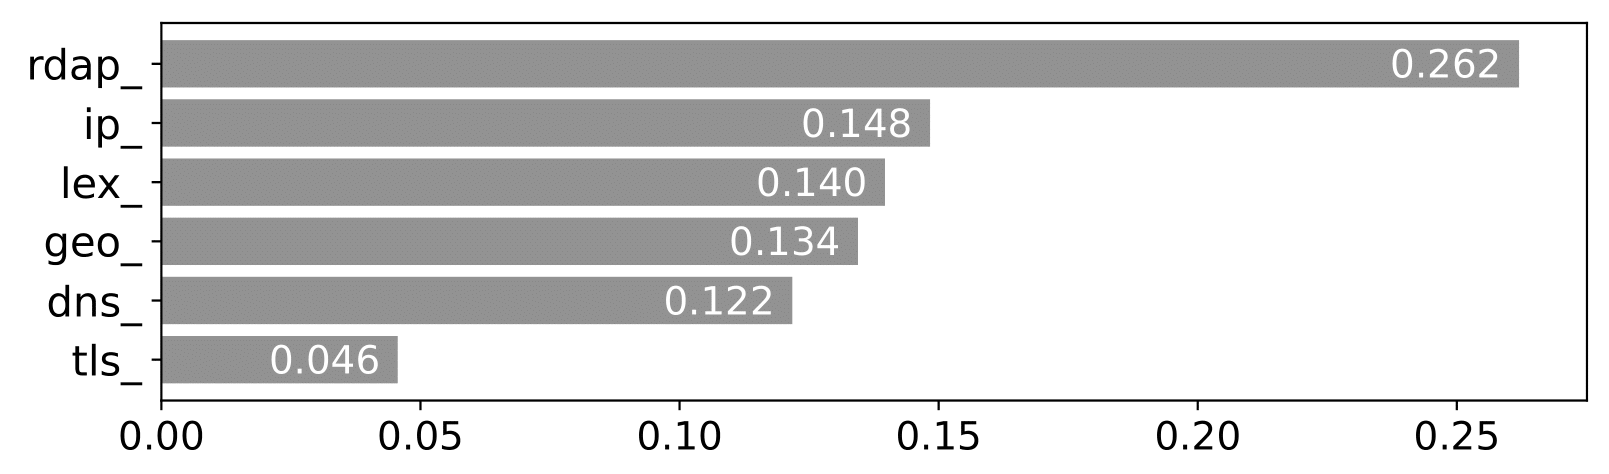
\includegraphics[width=\linewidth,clip]{obrazky-figures/cropped_shap.png}
    \caption{Agregovaný přínos kategorií příznaků dle hodnot analýzy SHAP vypočtených pro LightGBM model. Výsledky vycházejí z~podmnožiny dat použité v~publikaci Spotting the Hook~\cite{CNSM}.}
    \label{fig:aggregated-shap}
\end{figure}

Tento rozbor potvrzuje, že efektivní detekce phishingu nelze postavit pouze na jedné kategorii dat, ale vyžaduje kombinaci více zdrojů. Zároveň zdůrazňuje potřebu cíleného rozšiřování klíčových kategorií a optimalizace méně přínosných oblastí.


\subsection{Strategie dalšího rozšiřování}

Na základě těchto poznatků byla metodologie rozšíření příznaků formulována následovně:

\begin{enumerate} \item \textbf{Prioritizace expanze RDAP a IP příznaků:} Bylo navrženo doplnění nových atributů zaměřených na registrátory, DNSSEC podporu, entropii IP prefixů a geografickou diverzitu. \item \textbf{Detailní analýza LEX příznaků:} Probíhá rozšiřování \textit{n}-gramových shod a výpočty specifických skóre rizikovosti na základě doménového jména. \item \textbf{Doplňková optimalizace DNS příznaků:} Sběr specifických parametrů TTL a analýza variability v~čase. \item \textbf{Kritická revize TLS příznaků:} Vzhledem k~nízkému přínosu bylo rozhodnuto zaměřit se pouze na selektivní rozšíření těch atributů, které prokazatelně korelují s~podvodnými doménami (např. délka certifikátu, typ cipheru). \end{enumerate}

\noindent Tento postup je dále podložen experimentálními výsledky z~práce Hranického a kol. \cite{CNSM}, kde bylo prokázáno, že kombinace více zdrojů informací výrazně snižuje míru falešných pozitivních detekcí a zvyšuje robustnost klasifikátorů.

\subsection{Shrnutí a hlavní přínosy}

Metodologie tvorby příznaků navazuje na předchozí vývoj a vychází z~poznatků publikovaných v~rámci práce Hranického et al. \cite{CNSM}, která se zaměřuje na využití doménových dat pro pokročilou detekci phishingu.

\begin{itemize} \item Využití pěti nezávislých datových zdrojů (DNS, RDAP, IP, GEO, TLS). \item Detailní analýzu přínosu jednotlivých kategorií pomocí metody SHAP. \item Cílenou expanzi klíčových příznaků a optimalizaci slabších oblastí. \item Experimentální ověření dopadu příznaků na skóre F1 a míru falešně pozitivních výsledků. \end{itemize}

\noindent Výsledky ukazují, že pečlivý feature engineering zásadním způsobem ovlivňuje úspěšnost detekce phishingových domén a představuje klíčovou komponentu každého moderního systému kybernetické bezpečnosti.



\chapter{Předběžná analýza podmnožin příznaků}
\label{chapter:7}

Předběžná analýza byla provedena s~cílem identifikovat nejpřínosnější skupiny příznaků pro detekci škodlivých doménových jmen. Bylo zkoumáno, podle kterých charakteristik je vhodné provádět klasifikaci a které modely poskytují nejpřesnější výsledky. Na základě těchto měření byly následně definovány výsledné skupiny příznaků a zvoleny nejvhodnější klasifikátory.


Pro automatizaci procesu trénování a porovnání modelů byla využita knihovna \texttt{PyCaret}, která umožňuje rychlé testování různých klasifikačních algoritmů na daných sadách příznaků. Pro každé měření jsou provedeny následující kroky:

\begin{enumerate}
    \item Nastavení prostředí pro trénování modelů v~knihovně \texttt{PyCaret}.
    \item Pro každou skupinu příznaků se spustí trénovací proces s~cílem maximalizovat \textit{skóre F1}.
    \item Jsou vybrány tři nejlepší modely pro každou skupinu a uloží se jejich výsledky.
    \item Výsledky jsou následně agregovány do jedné tabulky pro lepší přehlednost.
\end{enumerate}

\section{Skupiny příznaků}


Pro každou skupinu příznaků uvedenou výše \ref{item:segment} byla provedena série experimentů, v~rámci nichž bylo testováno deset různých klasifikačních algoritmů. Dále budou použity zkratky, jejichž plný výčet se nachází níže:

\begin{itemize}
    \item \texttt{RF} – Random Forest,
    \item \texttt{ET} – Extra Trees,
    \item \texttt{KNN} – K-Neighbors Classifier,
    \item \texttt{XGB} – XGBoost,
    \item \texttt{LGBM} – LightGBM,
    \item \texttt{DT} – Decision Tree,
    \item \texttt{GB} – Gradient Boosting,
    \item \texttt{ADA} – AdaBoost,
    \item \texttt{LDA} – Linear Discriminant Analysis,
    \item \texttt{Ridge} – Ridge Classifier,
    \item \texttt{LR} – Logistic Regression,
    \item \texttt{Dummy} – Dummy Classifier,
    \item \texttt{SVM} – Support Vector Machine (Linear),
    \item \texttt{QDA} – Quadratic Discriminant Analysis,
    \item \texttt{NB} – Naive Bayes
\end{itemize}


\subsection{Seskupování}

Jak bylo popsáno v~sekci \ref{subsection:colect}, systém DomainRadar implementuje segmentovaný proces sběru dat, v~rámci kterého jsou doménová jména postupně obohacována o~různé typy informací (DNS odpovědi, RDAP záznamy, TLS certifikáty apod.). Tento architektonický přístup znamená, že \textbf{ne vždy jsou k~dispozici všechny druhy dat pro každou doménu}.  
V~praxi proto vzniká potřeba pracovat s~více úrovněmi kompletnosti dat – tzv. \textbf{podmnožiny}.

Na základě charakteru sběru a dostupnosti dat byly definovány tři hlavní podmnožiny příznaků:

\begin{enumerate}
    \item \textbf{Pouze lexikální příznaky (\texttt{["lex\_"]})} – Tato podmnožina zahrnuje pouze informace vycházející z~názvu domény samotné. Jelikož každé doménové jméno je alespoň známé, představují lexikální příznaky nejzákladnější a vždy dostupnou variantu.
    
    \item \textbf{Lexikální + DNS + IP + geolokační příznaky (\texttt{["lex\_", "dns\_", "ip\_", "geo\_"]})} – Tato podmnožina je dostupná, pokud se podaří provést úspěšnou DNS rezoluci doménového jména na IP adresu. Na základě IP adresy lze následně obohatit data o~geolokační informace. Tyto příznaky jsou sbírány zároveň (viz schéma sběru DomainRadar na Obrázku~\ref{fig:domainradar_flow}) a jejich získání je zpravidla rychlé a nenáročné.
    
    \item \textbf{Plná data (\texttt{["lex\_", "dns\_", "ip\_", "tls\_", "geo\_", "rdap\_"]})} – Nejkomplexnější varianta, obsahující kromě předchozích příznaků také informace z~TLS certifikátů a RDAP protokolu. Tato podmnožina umožňuje dosáhnout nejvyšší přesnosti klasifikace, protože kombinuje široké spektrum technických a registračních dat. Je však dostupný pouze pro domény, pro které byl sběr těchto pokročilých dat úspěšný.
\end{enumerate}

Výběr konkrétní podmnožiny příznaků pro klasifikaci závisí na úspěšnosti sběru dat.  
\textbf{V~případě neúplných dat je provedena klasifikace pomocí nejvyšší kompletní podmnožiny.}  
Například pokud není dostupný RDAP záznam, ale je známá IP adresa a geolokační údaje, použije se podmnožina \texttt{["lex\_", "dns\_", "ip\_", "geo\_"]}.  
Pokud selže i DNS rezoluce, využijí se pouze lexikální příznaky.

Tento přístup umožňuje maximalizovat využitelnost nasbíraných dat a zajistit, že každé doménové jméno bude klasifikováno s~nejvyšší možnou mírou detailu, kterou dostupná data umožňují.




\section{Výsledky měření}

Celkem bylo provedeno 420 měření, přičemž každá metoda byla aplikována na 42 různých datových sad, zahrnujících jednotlivé skupiny příznaků a jejich případné agregace. 

Kvůli přehlednosti vizualizací byla zavedena následující tabulka pro překlad jednotlivých agregací:


\begin{table}[ht]
  \centering

  \begin{tabular}{|l|l|r|r|}
    \toprule
    Zkratka & Klíč & \# příznaků & \# vzorků \\
    \midrule
    Lex & \texttt{lex} & 63 & 649037 \\
    Lex+dns+ip & \texttt{lex\_+dns\_+ip} & 111 & 649037 \\
    Lex+...+geo & \texttt{lex\_+dns\_+ip\_+geo} & 129 & 649037 \\
    Lex+...+tls & \texttt{lex\_+dns\_+ip\_+tls\_+geo} & 153 & 649037 \\
    Lex+...+rdap & \texttt{lex\_+dns\_+ip\_+tls\_+geo\_+rdap} & 177 & 649037 \\
    Lex+...+html & \texttt{lex\_+dns\_+ip\_+tls\_+geo\_+rdap\_+html} & 264 & 49037 \\
    \bottomrule
  \end{tabular}
    \caption{Překlad popisů agregací skupin příznaků}
  \label{tab:subset-lookup}
\end{table}


\noindent Výsledky měření můžeme rozdělit do tří částí:
\begin{itemize}
    \item Samostatné skupiny příznaků - Pouze na základě izolovaných skupin příznaků dle jejich původu.  
    \item Agregované skupiny příznaků - Postupné agregování příznaků. 
    \item Logické stupňování příznaků - Dle pořadí sběru. 
\end{itemize}

\noindent Definici jednotlivých segmentů příznaků nalezneme výše v~sekci \hyperref[item:segment]{Segmentace}. Pro ilustraci struktury měření je uveden příklad výsledků dosažených na podmnožině \texttt{dns} pro malwar domény:

\begin{table}[H]
    \centering
    \begin{tabular}{|l|c|c|c|c|c|c|c|c|}
    \hline
    \textbf{Model} & \textbf{Acc} & \textbf{AUC} & \textbf{Rec} & \textbf{Prec.} & \textbf{F1} & \textbf{Kappa} & \textbf{MCC} & \textbf{TT (s)} \\
    \hline
    \texttt{RF} & 0.9165 & 0.9120 & 0.9165 & 0.9135 & 0.9143 & 0.6861 & 0.6886 & 1.80 \\
    \texttt{ET} & 0.9155 & 0.8910 & 0.9155 & 0.9125 & 0.9133 & 0.6829 & 0.6851 & 0.45 \\
    \texttt{KNN} & 0.9142 & 0.8860 & 0.9142 & 0.9109 & 0.9116 & 0.6757 & 0.6787 & 0.24 \\
    \texttt{XGB} & 0.9166 & 0.9175 & 0.9166 & 0.9129 & 0.9115 & 0.6681 & 0.6785 & 0.44 \\
    \texttt{LGBM} & 0.9174 & 0.9176 & 0.9174 & 0.9144 & 0.9113 & 0.6647 & 0.6794 & 0.61 \\
    \texttt{DT} & 0.8958 & 0.8503 & 0.8958 & 0.8957 & 0.8957 & 0.6268 & 0.6271 & 0.19 \\
    \texttt{GB} & 0.8911 & 0.8799 & 0.8911 & 0.8921 & 0.8728 & 0.4991 & 0.5538 & 2.77 \\
    \texttt{ADA} & 0.8632 & 0.8417 & 0.8632 & 0.8536 & 0.8335 & 0.3352 & 0.3997 & 0.71 \\
    \texttt{LDA} & 0.8491 & 0.7843 & 0.8491 & 0.8264 & 0.8136 & 0.2532 & 0.3100 & 0.17 \\
    \texttt{Ridge} & 0.8346 & 0.7842 & 0.8346 & 0.7962 & 0.7724 & 0.0722 & 0.1401 & 0.12 \\
    \texttt{LR} & 0.8242 & 0.6988 & 0.8242 & 0.7307 & 0.7582 & 0.0143 & 0.0262 & 1.31 \\
    \texttt{Dummy} & 0.8317 & 0.5000 & 0.8317 & 0.6917 & 0.7553 & 0.0000 & 0.0000 & 0.06 \\
    \texttt{SVM} & 0.6466 & 0.6454 & 0.6466 & 0.7720 & 0.6756 & 0.1180 & 0.1475 & 0.14 \\
    \texttt{QDA} & 0.5847 & 0.7880 & 0.5847 & 0.8468 & 0.6332 & 0.2208 & 0.3161 & 0.14 \\
    \texttt{NB} & 0.3432 & 0.6313 & 0.3432 & 0.8202 & 0.3546 & 0.0640 & 0.1513 & 0.07 \\
    \hline
    \end{tabular}
    \caption{Výsledky modelů pro podmnožinu DNS (malware); modely označeny zkratkami}
    \label{tab:malware_dns_results}
\end{table}

Kompletní výsledky všech měření a porovnání modelů pro ostatní podmnožiny jsou uvedeny v~příloze \ref{sec:appendix-results}.


\subsection{Samostatné skupiny příznaků}
\label{subsection:standalone_res}

V~první sérii experimentů byla každá kategorie příznaků testována samostatně. Cílem bylo zjistit, které jednotlivé typy informací (např. pouze TLS, pouze DNS, pouze LEX) nesou největší diskriminační sílu při klasifikaci škodlivých domén. Výsledky měření ukázaly, že nejvyšší úspěšnosti v~samostatných skupinách dosahovaly:
\begin{itemize}
    \item \textbf{RDAP příznaky} – zejména díky atributům souvisejícím s~věkem a registrací domén,
    \item \textbf{DNS příznaky} – hlavně v~oblasti TTL hodnot a četnosti typů záznamů,
    \item \textbf{IP příznaky} – entropie IP prefixů a diverzita autonomních systémů.
\end{itemize}

Podrobné výsledky pro malware a phishing domény nalezneme na ilustracích ~\ref{fig:subset_phish_results} a~\ref{fig:subset_malware_results}.


\begin{figure}[!h]
    \centering
    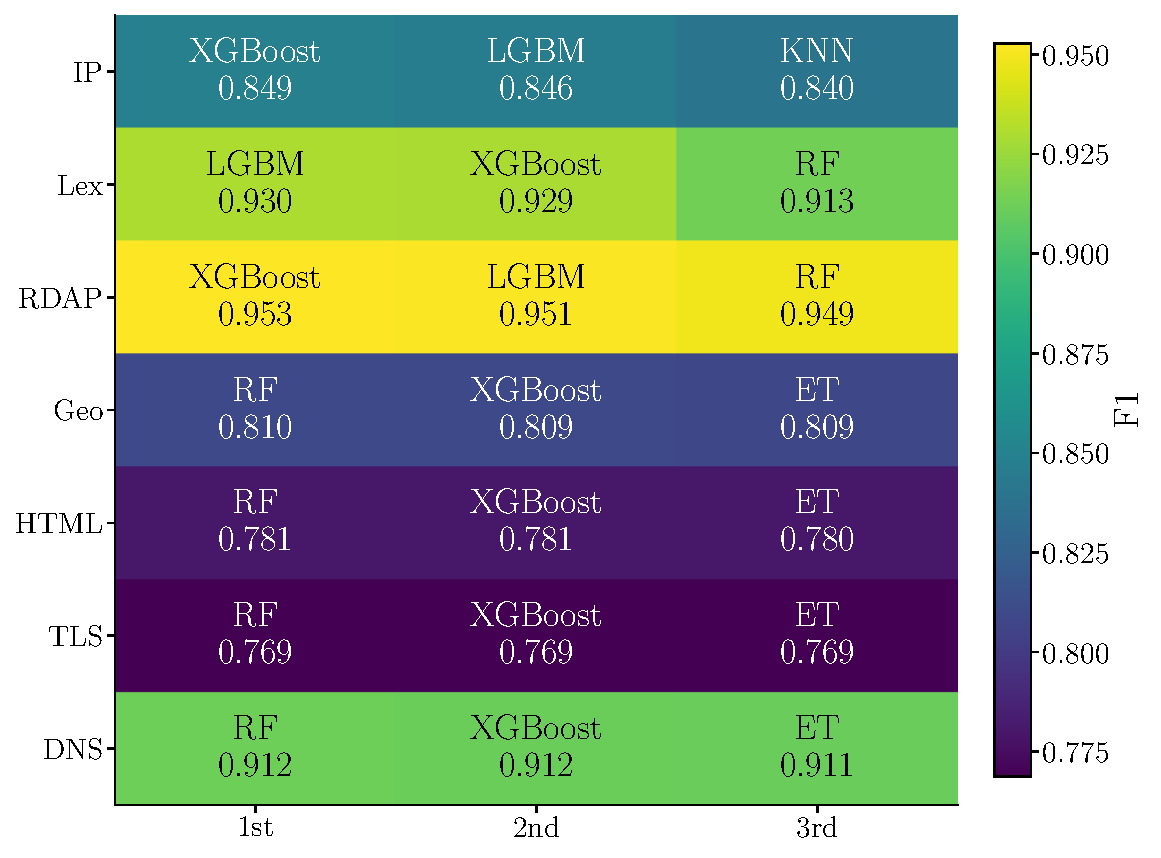
\includegraphics[width=\textwidth]{obrazky-figures/base_phishing.pdf}
    \caption{Výsledky měření samostatných podmnožin – phishing.}
    \label{fig:subset_phish_results}
\end{figure}

\begin{figure}[!h]
    \centering
    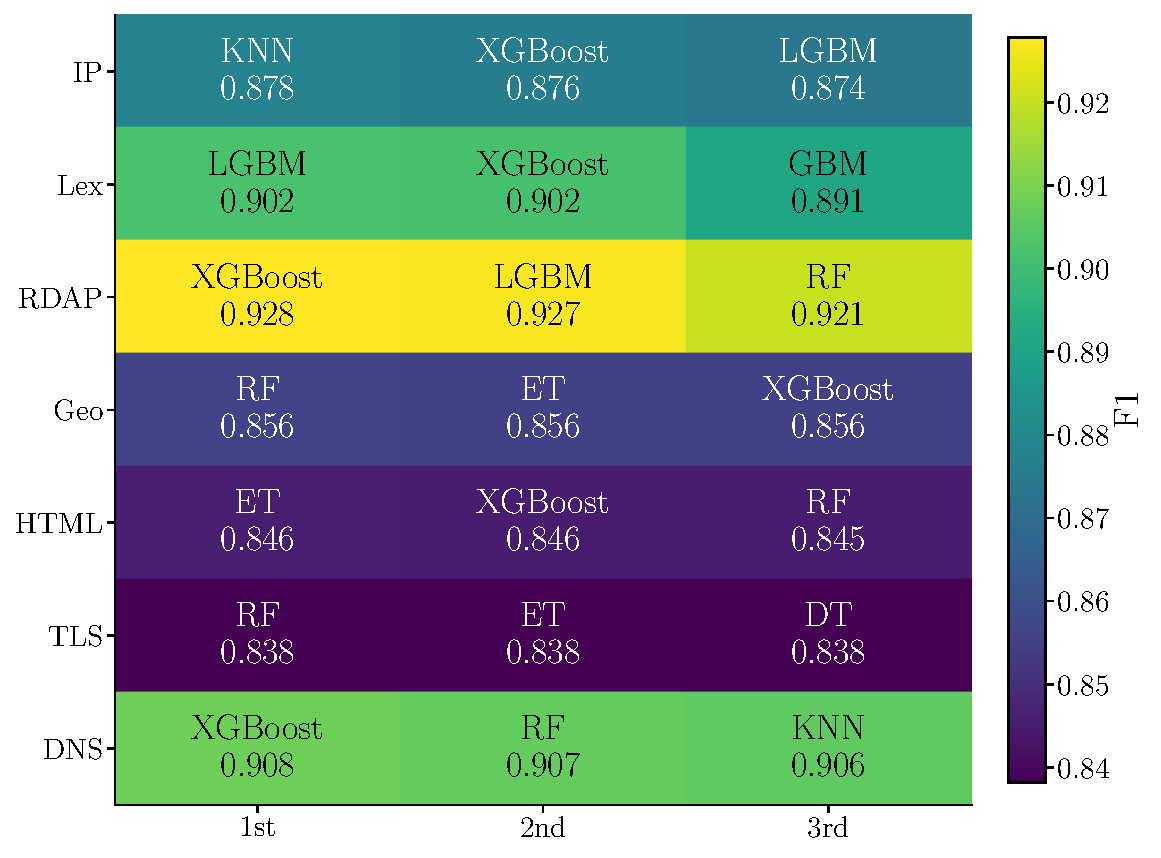
\includegraphics[width=\textwidth]{obrazky-figures/base_malware.pdf}
    \caption{Výsledky měření samostatných podmnožin – malware.}
    \label{fig:subset_malware_results}
\end{figure}

\subsection{Agregované skupiny příznaků}
\label{subsection:agg_res}


Ve druhé fázi experimentů byly jednotlivé skupiny příznaků agregovány dohromady. Cílem bylo ověřit, jak kombinace více zdrojů informací ovlivňuje klasifikační úspěšnost.

Agregované výsledky ukazují, že kombinace příznaků napříč kategoriemi  výrazně zvyšuje skóre F1 oproti použití samostatných skupin. Nejvyšší dosažené hodnoty \textit{skóre F1} dosáhly 0.9880 pro phishing a 0.9850 pro malware. Zajímavým zjištěním je také to, že přidání poslední skupiny příznaků, tedy HTML, nezvýší přesnost klasifikace. 

Pro každou kombinaci příznakových skupin (řádky Lex až Lex+...+html) jsou zobrazeny tři nejlepší klasifikátory (sloupce 1st–3rd). Barevná paleta („heatmap“) indikuje hodnotu skóre F1 – tmavší buňka znamená vyšší skóre. Na buňkách jsou vytištěny zkratky modelů (RF, ADA, DT, …, ET) a přesné F1 hodnoty na tři desetinná místa. Výsledky agregovaných podmnožin jsou znázorněny na obrázcích~\ref{fig:aggregate_phish_results} a~\ref{fig:aggregate_malware_results}.

\clearpage                  % nebo \cleardoublepage pokud děláte twoside
\begin{figure}[!h]
    \centering
    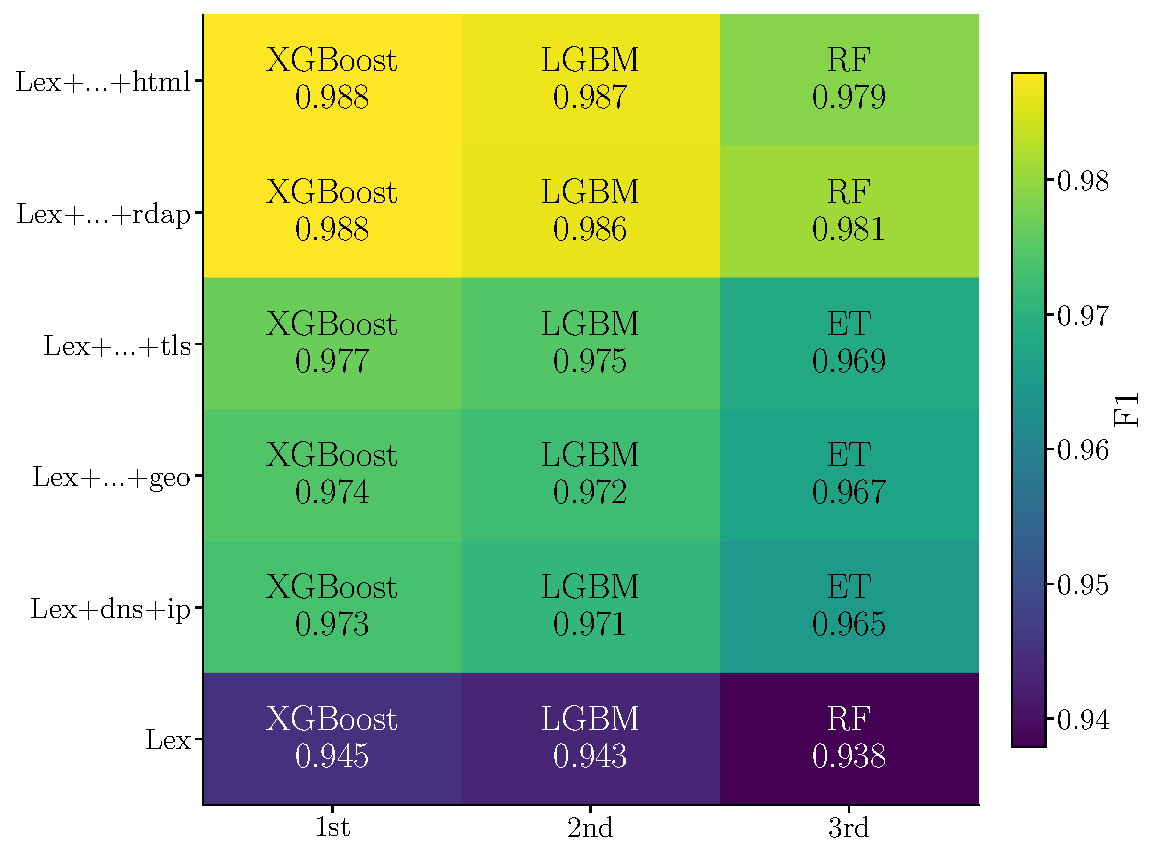
\includegraphics[width=\columnwidth]{obrazky-figures/agg_phishing.pdf}
    \caption{Výsledky měření agregovaných subsetů – phishing.}
    \label{fig:aggregate_phish_results}
\end{figure}
 
\begin{figure}[!h]
    \centering
    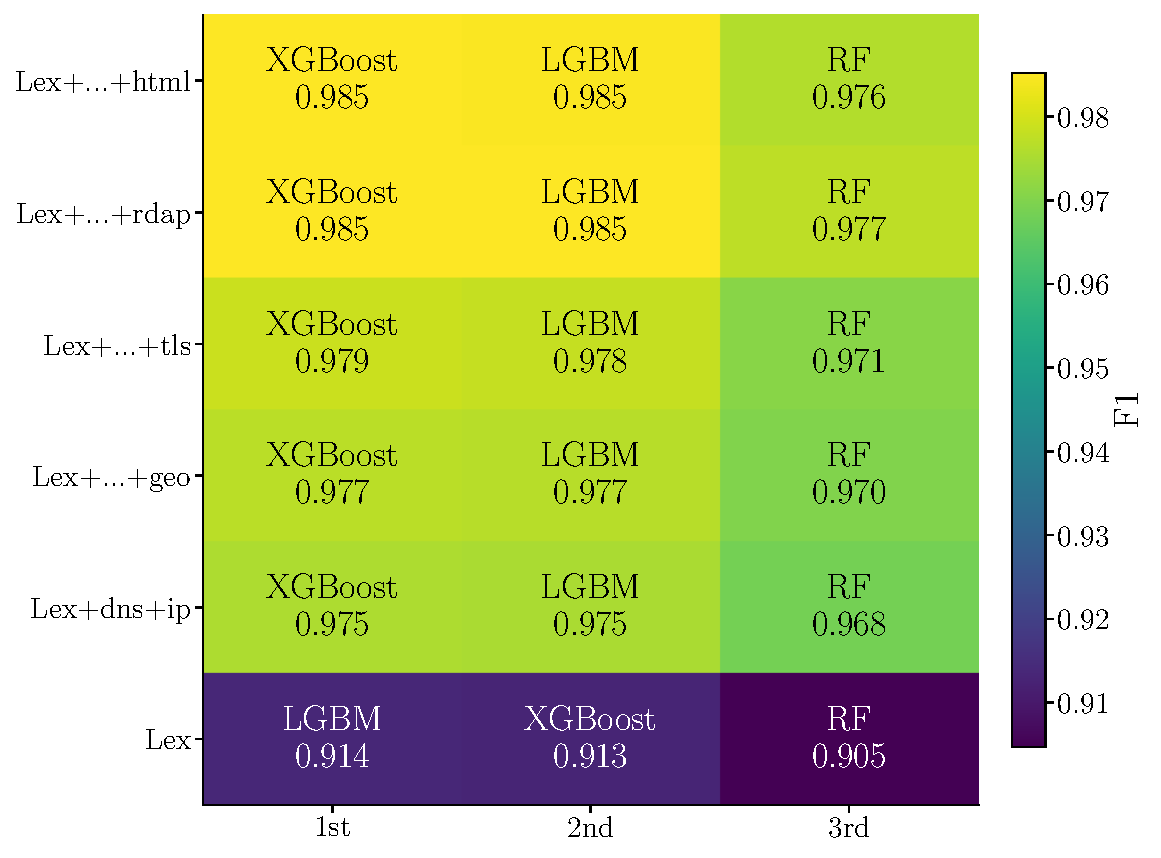
\includegraphics[width=\columnwidth]{obrazky-figures/agg_malware.pdf}
    \caption{Výsledky měření agregovaných subsetů – malware.}
    \label{fig:aggregate_malware_results}
\end{figure}



\subsection{Logické stupňování příznaků}
\label{logi_step}

Ve třetí sadě experimentů byla testována strategie postupného rozšiřování vektoru příznaků, vycházející z~architektury nástroje \texttt{DomainRadar}. Příznaky byly přidávány v~následujících fázích:

\begin{enumerate}
    \item Pouze \texttt{lex} příznaky (minimální sběr dat).
    \item Kombinace \texttt{lex + dns + ip + tls + geo}. Vynechán náročný sběr RDAP a HTML. 
    \item Plná kombinace všech skupin: \texttt{lex + dns + ip + tls + geo + rdap}.
\end{enumerate}

Tento stupňovitý přístup reflektuje implementaci systému Domainradar \cite{domainradar}, stejně tak i náročnost sběru jednotlivých skupin příznaků. 

Výsledky rozšiřování vstupního vektoru dat hraje velmi významnou roli v~přesnosti klasifikace, avšak jen do určité meze. Přidáním HTML příznaků se dle měření přesnost nijak nezvýší. 

Výsledky pro tento přístup jsou uvedeny v~předchozí sekci, neboť se  jedná o~podmnožinu všech postupných podmnožin. 


\clearpage

\section{Shrnutí}
Závěry měření jsou tedy následující:

\begin{itemize}
    \item Samostatné podmnožiny poskytují užitečné informace, ale jejich kombinace výrazně zvyšuje úspěšnost detekce.
    \item Nejvyššího \textit{skóre F1} bylo dosaženo při použití agregovaných příznaků ze všech dostupných zdrojů.
    \item Postupné rozšiřování vektoru příznaků podle dostupnosti dat přináší stabilní zlepšování výsledků.
    \item Nejlepšími klasifikátory napříč všemi experimenty byly \textbf{Extreme Gradient Boosting (XGBoost)}, \textbf{LightGBM} a \textbf{Random Forest}.
    \item HTML příznaky mají pouze minimální přínos. 
\end{itemize}


Z~Obrázku~\ref{fig:avg_models} je zřejmé, že nejvyšší průměrné skóre F1 dosahují klasifikátory \textbf{LightGBM} a \textbf{XGBoost}. Tyto dva modely byly proto zvoleny pro další fázi vývoje finálního klasifikačního systému.

\begin{figure}[h]
  \centering
  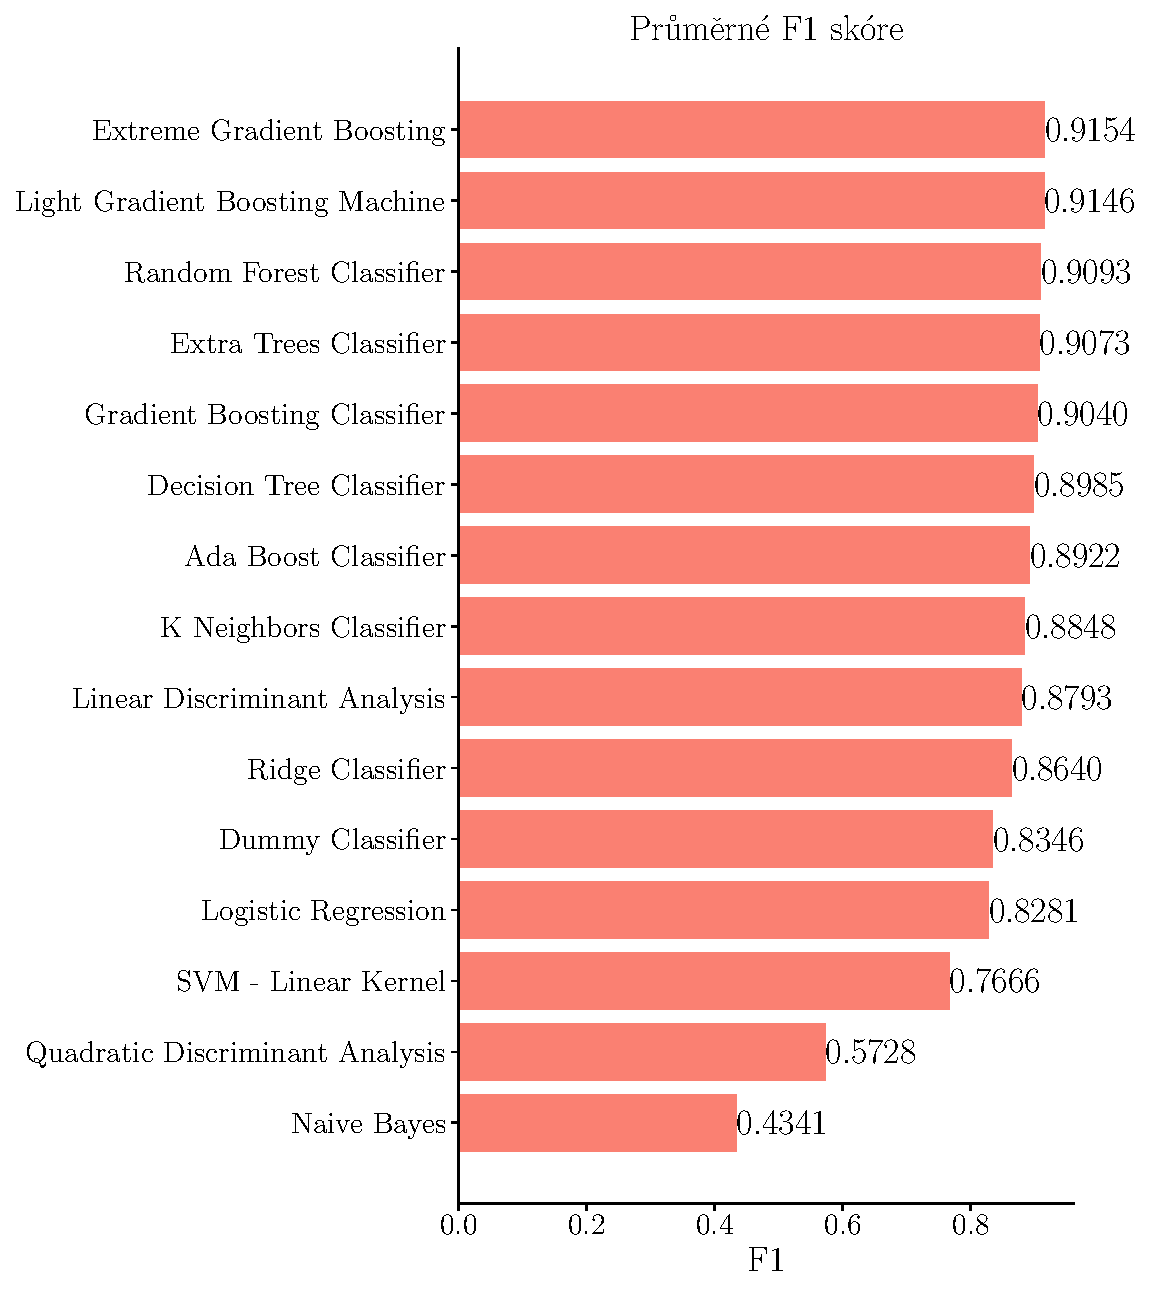
\includegraphics[width=0.8\columnwidth]{obrazky-figures/average_f1_models.pdf}
  \caption{Průměrné skóre F1 jednotlivých klasifikátorů napříč podmnožinami.}
  \label{fig:avg_models}
\end{figure}


\chapter{Návrh a implementace klasifikátorů}
\label{chapter:8}


Účinná detekce maligních domén vyžaduje promyšlenou kombinaci různých klasifikačních přístupů, které dokáží pružně reagovat na variabilitu dostupných dat a rychle se měnící charakter kybernetických hrozeb. V~této kapitole je podrobně popsán návrh modulární klasifikační pipeline, která zahrnuje více úrovní rozhodování a využívá kombinovaný přístup ke zvýšení přesnosti a robustnosti detekce.

Cílem kapitoly je představit jednotlivé modely, které tvoří stavební bloky této pipeline – včetně stromových algoritmů (XGBoost, LightGBM), neuronových sítí (FFNN, CNN) i specializovaných modulů (TLS klasifikátor, metamodel, FPD). Zvláštní důraz je kladen na to, jak jsou tyto modely navrženy, trénovány a integrovány do víceúrovňového systému rozhodování.

Zásadní roli hraje rozdělení vstupních domén podle množství dostupných příznaků do tří úrovní (\textit{stages}). Každé úrovni odpovídá specifická sada klasifikátorů optimalizovaných na daný rozsah informací. Výsledky modelů jsou následně agregovány pomocí metaklasifikátoru. Pro zvýšení spolehlivosti je do procesu začleněn i doplňkový modul pro detekci falešně pozitivních případů (FPD), který dále filtruje podezřelé predikce. Tato kapitola zahrnuje:
\begin{itemize}
    \item Detailní popis jednotlivých klasifikačních modelů, jejich architektur a použitých technik trénování.
    \item Vysvětlení principu vícestupňové klasifikace podle dostupnosti dat a způsobu výběru příslušných modelů.
    \item Popis strategie agregace výstupů více modelů pomocí vážení, hlasování nebo metaklasifikace.
    \item Integraci modulu FPD pro dodatečnou eliminaci falešně pozitivních detekcí.
    \item Optimalizační strategie pro výběr hyperparametrů a zvýšení robustnosti klasifikátorů.
\end{itemize}

\noindent Všechny komponenty byly navrženy s~ohledem na škálovatelnost, adaptabilitu a snadnou integraci do reálného bezpečnostního systému. Výsledná pipeline umožňuje flexibilní klasifikaci i v~případech s~neúplnými daty a minimalizuje riziko chybné detekce díky kombinaci více rozhodovacích vrstev. Kapitola tak nabízí ucelený pohled na návrh pokročilého systému pro detekci škodlivých domén a poskytuje rámec pro jeho další rozvoj či nasazení v~praxi.

\section{XGBoost}

V~této sekci je popsán návrh, implementace a konfigurace modelu XGBoost pro detekci maligních domén. Samotné experimentální výsledky dosažené tímto modelem jsou prezentovány v~kapitole \ref{experiments:eval}, konkrétně v~sekci \ref{res:xgb}.

XGBoost (Extreme Gradient Boosting) je výkonný open-source algoritmus pro gradient boosting, který si získal významné postavení v~oblasti strojového učení díky své vysoké efektivitě, přesnosti a schopnosti práce s~rozsáhlými a nevyváženými datovými sadami. Klíčovými vlastnostmi jsou podpora paralelních výpočtů, možnost zabudované regularizace (L1, L2) a flexibilní správa paměti, což je činí ideálním pro úlohy detekce škodlivých domén \cite{chen2016xgboost}. 


\subsection{Předzpracování dat}

Pro trénování modelu XGBoost byla využita  sada transformací popsaná v~sekci~\ref{general_transformation}. Vstupní data byla upravena následujícím způsobem:
\begin{itemize}
    \item Odstranění chybějících hodnot (nahrazení nulou).
    \item Převedení binárních příznaků na celočíselné hodnoty (0/1).
    \item Min-max škálování všech numerických atributů do intervalu $[0, 1]$.
    \item Odstranění extrémních hodnot podle pravidla založeného na odchylce od průměru.
\end{itemize}

\noindent Tyto kroky zajistily stabilní a konzistentní vstupní reprezentaci vhodnou pro trénování stromových modelů bez výrazného zkreslení distribuce příznaků.

\subsection{Architektura a hyperparametry modelu}

Model XGBoost byl konfigurován s~následujícími hyperparametry:
\begin{itemize}
    \item \textbf{Počet stromů (n\_estimators)}: \texttt{300}
    \item \textbf{Maximální hloubka stromu (max\_depth)}: \texttt{9}
    \item \textbf{Rychlost učení (learning\_rate)}: \texttt{0.023}
    \item \textbf{Subsampling poměr (subsample)}: \texttt{0.8}
    \item \textbf{Regulace L2 (lambda)}: \texttt{1.5}
    \item \textbf{Minimální váha listu (min\_child\_weight)}: \texttt{1.0}
\end{itemize}

\noindent Hyperparametry byly optimalizovány pomocí Bayesovské optimalizace na validační sadě s~cílem maximalizovat skóre F1. Tato metoda umožnila efektivně prohledat prostor parametrů a nalézt nastavení vedoucí k~optimálním výsledkům i při relativně omezeném počtu experimentů ~\cite{snoek2012practical}.

Jednou z~hlavních výhod použití XGBoost v~této aplikaci je jeho schopnost efektivně pracovat s~nerovnováhou tříd v~datech a vysoká odolnost vůči šumu. Díky interní implementaci L1 a L2 regularizace model dosahuje lepší generalizace, což je kritické v~dynamicky se měnících podmínkách detekce kybernetických hrozeb ~\cite{chen2016xgboost}.

Model XGBoost zároveň umožňuje snadnou interpretaci výsledků pomocí výstupů významnosti jednotlivých příznaků (feature importance), což je důležité při dalším ladění a zlepšování detekčních mechanismů ~\cite{lundberg2017unified}.

\subsubsection{Výhody XGBoost v~detekci domén}
XGBoost se vyznačuje vysokou škálovatelností ve všech scénářích, což je zvláště důležité v~oblasti detekce domén, kde se často pracuje s~rozsáhlými a různorodými datovými sadami. Paralelní a distribuované výpočty, které algoritmus podporuje, umožňují rychlejší učení a zpracování velkých objemů dat, což je klíčové pro efektivní identifikaci potenciálně škodlivých nebo podezřelých doménových jmen.~\cite{chen2016xgboost}.





\section{LightGBM}

Tato sekce se zaměřuje na návrh, implementaci a konfiguraci modelu LightGBM pro úlohu detekce maligních domén. Experimentální výsledky získané tímto modelem jsou uvedeny v~kapitole \ref{experiments:eval} v~sekci \ref{res:lgbm}.

LightGBM (Light Gradient Boosting Machine) je efektivní algoritmus založený na gradient boostingu, který je optimalizován pro rychlé trénování a nízkou spotřebu paměti. Díky své schopnosti zpracovávat velké objemy dat a práci se sparse strukturami je vhodným kandidátem pro aplikace v~oblasti detekce kybernetických hrozeb. \cite{ke2017lightgbm}


\subsection{Předzpracování dat}

Předzpracování dat pro model LightGBM vycházelo ze stejných principů jako u~XGBoost, v~souladu s~transformacemi uvedenými v~sekci~\ref{general_transformation}. Aplikovány byly následující kroky:
\begin{itemize}
    \item Náhrada chybějících hodnot nulou.
    \item Převedení binárních atributů na numerickou reprezentaci.
    \item Normalizace všech numerických příznaků metodou min-max.
    \item Odstranění odlehlých hodnot na základě směrodatné odchylky.
\end{itemize}

\noindent Tím bylo dosaženo jednotného formátu vstupních dat, který minimalizuje zkreslení a zvyšuje robustnost modelu při trénování.


\subsection{Architektura a hyperparametry modelu}

Model LightGBM byl trénován s~následující konfigurací hyperparametrů:
\begin{itemize}
    \item \textbf{Počet stromů (n\_estimators)}: \texttt{600}
    \item \textbf{Maximální hloubka stromu (max\_depth)}: \texttt{12}
    \item \textbf{Rychlost učení (learning\_rate)}: \texttt{0.0978}
    \item \textbf{Subsampling poměr (subsample)}: \texttt{0.596}
    \item \textbf{Regulace L2 (lambda\_l2)}: \texttt{2.07}
    \item \textbf{Minimální váha listu (min\_child\_weight)}: \texttt{1.0}
    \item \textbf{Metoda vzorkování (sampling\_method)}: \texttt{gradient\_based}
    \item \textbf{Velikost koše (max\_bin)}: \texttt{512}
\end{itemize}

\noindent Parametry byly zvoleny na základě zkušeností z~ladění XGBoost modelu, s~drobnými úpravami pro optimalizaci \textbf{LightGBM}. Díky použití metody \textit{gradient-based sampling} model efektivněji vybírá vzorky během trénování, což umožňuje rychlejší konvergenci bez výrazné ztráty přesnosti ~\cite{ke2017lightgbm}.

Významnou výhodou LightGBM je také jeho schopnost efektivně pracovat se \textbf{sparse} daty a podporovat \textbf{kategorické atributy} nativně, bez nutnosti jejich explicitní transformace~\cite{ke2017lightgbm}. To umožňuje jednodušší a rychlejší předzpracování v~budoucích aplikacích.

Navíc díky technikám jako \textit{leaf-wise tree growth} dosahuje LightGBM \textbf{vyšší predikční přesnosti} než tradiční boostingové algoritmy, a to zejména v~případě komplexních a vysoce nelineárních úloh, jaké jsou typické při detekci škodlivých domén~\cite{ke2017lightgbm, zhao2020malicious}.







\section{Metoda podpůrných vektorů (SVM)}

Tato sekce popisuje návrh, implementaci a optimalizaci klasifikačního modelu SVM, který byl využit pro detekci maligních domén. Důraz je kladen na přípravu dat, konfiguraci modelu a detailní popis metod použitých pro ladění hyperparametrů. Výsledky trénování a testování jsou následně analyzovány v~kapitole \ref{experiments:eval}.

\subsection{Předzpracování dat}

Pro model Support Vector Machine (SVM) byla použita obecná schémata transformace popsaná v~sekci~\ref{general_transformation}. Důraz byl kladen na odstranění vlivu rozdílných měřítek příznaků, protože modely SVM jsou na tyto rozdíly citlivé. Aplikované kroky zahrnovaly:

\begin{itemize}
    \item Nahrazení chybějících hodnot nulou.
    \item Převedení binárních příznaků na celočíselné hodnoty.
    \item Min-max škálování do rozsahu $[0, 1]$.
    \item Odstranění odlehlých hodnot pomocí pravidla založeného na $2\sigma$ odchylce.
\end{itemize}

Tato forma předzpracování umožnila modelu efektivně pracovat s~daty bez zkreslení vlivem extrémních hodnot nebo nesrovnatelných rozsahů.


\subsection{Architektura modelu a výběr hyperparametrů}

Model byl implementován s~využitím jádra s~radiální bázovou funkcí (\textit{RBF kernel}). Vstupní parametry byly nastaveny následovně:

\begin{itemize}
    \item \textbf{Regularizační parametr $C$}: \texttt{59}
    \item \textbf{Parametr $\gamma$}: \texttt{0.1}
    \item \textbf{Typ jádra}: \texttt{rbf}
    \item \textbf{Vyvážení tříd}: \texttt{balanced}
    \item \textbf{Náhodný stav}: \texttt{42}
\end{itemize}

\noindent Optimalizace parametrů byla provedena pomocí \textbf{GridSearch}, jehož cílem bylo maximalizovat hodnotu \textit{skóre F1} na validační množině. Přestože GridSearch představuje systematický přístup k~výběru parametrů, jeho hlavní nevýhodou je značná výpočetní náročnost a nemožnost efektivního pokrytí celého parametrového prostoru při jeho velkém rozsahu. \cite{bergstra2011algorithms}. Vizualizaci prohledávaného prostoru pak můžeme nalézt na obrázku \ref{chart:grid_search}.

Z~tohoto důvodu byla v~rámci této práce implementována vlastní metoda \textbf{GradientGridSearch}, která kombinuje výhody GridSearch s~principy gradientního sestupu. Tato metoda předpokládá, že hodnoty blízké optimu poskytují podobně dobré výsledky a zaměřuje se na postupné zjemňování prostoru hledání. Implementace je uvedena v~algoritmu \ref{alg:gradient_grid_search}.

\begin{figure}[h!]
  \centering
  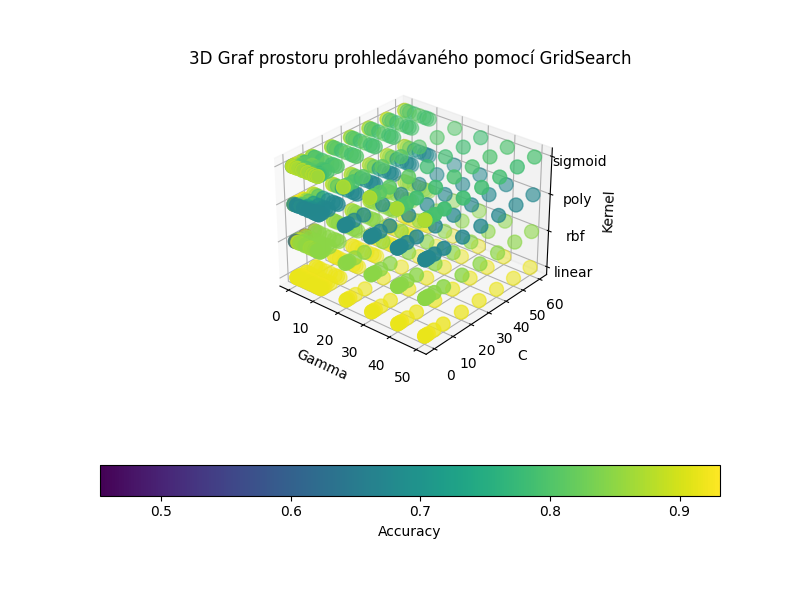
\includegraphics[width=1.0\textwidth]{obrazky-figures/grid.png}
  \caption{Vizualizace výsledků metodou GridSearch při hledání optimálních parametrů pro SVM.}
  \label{chart:grid_search}
\end{figure}


\subsection{Práce s~nevyváženými daty}

Vzhledem k~charakteru úlohy, kde většina domén je benigní a pouze malá část maligní, je datová sada značně nevyvážená. Tento stav vede ke zkreslení modelu směrem k~majoritní třídě. Proti tomuto efektu byla nasazena následující opatření:

\begin{itemize}
    \item Použití volby \texttt{class\_weight=balanced} v~rámci SVM.
    \item Úprava rozhodovacího prahu klasifikace.
    \item Testování různých metod převažování (např. \textit{SMOTE}) – i když nebyly přímo nasazeny v~konečné verzi modelu, posloužily jako důležitý kontrolní experiment.
\end{itemize}

\noindent Důvodem těchto opatření je snížení výskytu falešně pozitivních klasifikací, které by mohly vést k~chybnému zablokování legitimních domén.

\subsection{Specifika SVM v~doménové klasifikaci}

Model SVM se ukázal jako vhodný především pro klasifikaci podle lexikálních příznaků, které často nesou diskriminační hodnotu i v~případech, kdy chybí kontextové či síťové informace. V~rámci budoucího výzkumu se nabízí využití tohoto modelu jako součásti ansámblového klasifikátoru, nebo jeho kombinace s~online učením, jak ukazuje například přístup \textit{Feedback-SVM (F-SVM)} \cite{zou2019detecting}.

\subsection{Gradient Grid Search}

Gradient Grid Search je metoda optimalizace výběru parametrů pro SVM (Support Vector Machine), inspirovaná gradientním sestupem. 

Princip fungování algoritmu spočívá v~iterativním přibližování k~optimálním parametrům. Vnější smyčka kontroluje konvergenci a řídí globální pokrok algoritmu, zatímco vnitřní smyčka generuje nové kombinace parametrů na základě aktuálně nejlepší známé sady a provádí jejich evaluaci. Pokud nová kombinace přinese lepší výsledek, je tato kombinace akceptována jako nové výchozí řešení a následné kroky se orientují v~jejím okolí. S~každou iterací se také zmenšuje krok (parametr \texttt{alpha}), čímž se zpřesňuje prohledávání.

\noindent Tímto způsobem se efektivně zúží hledaný prostor a zrychluje se nalezení optimálních parametrů. Průběh je formálně znázorněn v~algoritmu~\ref{alg:gradient_grid_search}.


    \begin{algorithm}[h]
        \SetKwInOut{Input}{Input}
        \SetKwInOut{Output}{Output}
        \SetKwInOut{Initialize}{Initialize}
        \underline{function GGS}\;
        \Input{Initial SVM parameters, performance metrics}
        \Output{Optimized SVM parameters}
        \Initialize{Set alpha (step size), delta coefficient (new parameters factor)}
        
        Compute metrics for given parameters\;
        Set the best combination of parameters as current\;
        \While{not converged}{
            Generate a set of new parameters (delta) from the best combination\;
            \For{each parameter in delta}{
                Set parameter with step alpha\;
                Compute metrics for new parameter\;
                \If{new parameter's metric is better than current}{
                    Set new parameter as current\;
                    Update best combination of parameters\;
                }
            }
            Reduce alpha for next iteration\;
        }
        
         \label{alg:gradient_grid_search}
        \caption{Algoritmus Gradient Grid Search}       
    \end{algorithm}



\subsubsection{Analýza časové složitosti}
Analýza časové složitosti Gradient Grid Search (GGS) ukazuje, že je řízena hloubkou prohledávání a počtem iterací $k$ pro dosažení konvergence. Pro každou iteraci zkoumá $d$ nových kombinací parametrů, což vede k~složitosti $O(d \cdot k)$. Naproti tomu, pro tradiční GridSearch s~$n$ parametry a $m$ možnými hodnotami pro každý parametr je složitost $O(m^n)$.

\begin{align}
\text{Složitost GridSearch: } & O(m^n) \\
\text{Složitost GGS: } & O(d \cdot k) \\
\text{Dolní hranice GGS: } & O(d) \\
\text{Horní hranice GGS: } & O(d \cdot k_{\text{max}})
\end{align}

Zde $k_{\text{max}}$ označuje maximální počet iterací konvergence. Díky tomu, že GGS adaptivně zužuje prohledávaný prostor na základě dřívějších výsledků, je ve většině případů výrazně efektivnější než klasické plošné prohledávání.

Pro ilustraci uvažujme konkrétní případ optimalizace tří parametrů SVM: typu jádra (\texttt{kernel}) s~3 možnými hodnotami (lineární, polynomiální, RBF) a spojitých parametrů $C$ a $\gamma$, které jsou v~GridSearch discretizovány na 10 hodnot každé. Celkem by GridSearch musel vyhodnotit $3 \times 10 \times 10 = 300$ kombinací.

Naopak při použití GGS bychom mohli začít s~$d = 6$ počátečními kombinacemi (např. dvě pro každý typ jádra) a v~každé iteraci vyhodnotit 6 nových kombinací v~jejich okolí. Pokud by k~dosažení konvergence stačilo $k = 5$ iterací, vedlo by to k~celkovému počtu $6 \cdot 5 = 30$ vyhodnocených kombinací. Ve srovnání s~300 iteracemi GridSearchu by tedy GGS vyžadoval jen 10\,\% výpočetního času při podobné kvalitě výsledného modelu.

Tato úspora je podmíněna tím, že optimální oblast parametrů skutečně leží v~lokalizované části prostoru a že optimalizační funkce (typicky metrika výkonnosti modelu, např. skóre F1 nebo přesnost) je \textit{lokálně unimodální} a dostatečně hladká v~okolí optima. Jinými slovy, Gradient Grid Search implicitně předpokládá, že tato funkce má v~dané oblasti \textbf{monotonní gradient} směrem k~(lokálnímu) maximu a neobsahuje výrazné oscilace, které by mohly narušit konvergenci. Za těchto podmínek může být metoda velmi efektivní, protože postupné prohledávání prostoru parametrů vede ke zlepšování výstupu.

Je však důležité zdůraznit, že GGS nenabízí záruku nalezení globálního optima. Vzhledem k~deterministickému a lokálně orientovanému charakteru této metody může v~nehladkých nebo vícemodálních funkcích (s~více lokálními extrémy) snadno dojít k~uvíznutí v~suboptimálním řešení. V~takových případech je vhodné metodu rozšířit o~náhodnou inicializaci, restartování nebo hybridizaci s~globálními heuristikami (např. simulated annealing, evoluční algoritmy), které umožní únik z~lokálních extrémů a důkladnější prohledání celého prostoru.









% Aditional classifiers 

\section{Neuronové sítě}

Ačkoliv neuronové sítě představují velmi výkonnou třídu modelů pro detekci složitých vzorců v~datech, nebyly zahrnuty do předběžné analýzy podmnožin příznaků \ref{chapter:7}, jelikož nejsou podporovány přímo v~knihovně \texttt{PyCaret}, která byla použita pro automatizované testování klasifikátorů. Navíc jejich použití vyžaduje specifické předzpracování dat, například formátování do sekvenčních nebo obrazových struktur, normalizaci a úpravu dimenzionality vstupních atributů.

Přestože tento přístup neumožňuje přímé porovnání neuronových sítí s~modely jako XGBoost nebo LightGBM na úrovni frameworku PyCaret, jejich výjimečná schopnost modelovat nelineární vztahy a identifikovat komplexní struktury v~datech z~nich činí silné kandidáty pro detekci maligních domén.

V~rámci této práce byly navrženy a experimentálně ověřeny dva typy neuronových sítí, přičemž každý z~nich reflektuje specifický způsob reprezentace dat:

\begin{itemize}

        \item \textbf{Konvoluční neuronové sítě (CNN)} – aplikovány na 2D transformované atributové vektory, kde doménové vlastnosti jsou převedeny do podoby obrazu. CNN jsou schopné zachytit prostorové vzory a lokální korelace mezi příznaky. Podobný přístup byl úspěšně aplikován například v~práci Silveira et al. \cite{silveira2021detection}.
    
    \item \textbf{Klasické plně propojené neuronové sítě (Feedforward NN)} – využívají vektorovou reprezentaci doménových atributů bez strukturální transformace. Tento typ sítě slouží jako referenční architektura pro porovnání efektivity hlubokého učení na původní podobě dat \cite{ml_general}.
\end{itemize}

Každý z~těchto přístupů je v~následujících podsekcích detailně popsán včetně architektury, způsobu trénování, předzpracování dat a dosažených výsledků.



\section{Feedforward neuronová síť (FFNN)}

Plně propojené neuronové sítě (Feedforward Neural Networks, FFNN) představují základní architekturu hlubokého učení, kde se informace šíří jedním směrem – od vstupních vrstev přes skryté vrstvy až k~výstupní vrstvě. Přestože tyto sítě neobsahují rekurentní ani konvoluční prvky, při správném návrhu mohou efektivně modelovat složité vztahy v~datech, a to zejména v~případech, kdy jsou doménová data již vhodně předzpracovaná \cite{goodfellow2016deep}.

V~této sekci je popsán návrh a implementace plně propojené neuronové sítě určené pro klasifikaci maligních domén. Experimentální výsledky dosažené tímto modelem jsou uvedeny v~kapitole \ref{experiments:eval}, sekce \ref{res:feedforward}.

\subsection{Předzpracování dat}

Pro trénování plně propojené neuronové sítě (FFNN) byly využity transformační postupy popsané v~sekci~\ref{data-transform}, konkrétně kombinace obecných úprav a dodatečné sigmoidní transformace vhodné pro neuronové architektury.

\begin{itemize}
    \item Základní normalizace a čištění: nahrazení chybějících hodnot, převod binárních příznaků, min-max škálování.
    \item Odstranění odlehlých hodnot podle směrodatné odchylky.
    \item Aplikace sigmoidní transformace na vstupní atributy (viz sekce~\ref{sigmoid_transformation}), čímž byly hodnoty převedeny do hladkého intervalu $(0,1)$.
\end{itemize}

Použití sigmoidní funkce napomohlo stabilizaci gradientů a přispělo ke stabilnějšímu a rychlejšímu trénování neuronové sítě.

\subsection{Architektura feedforward sítě}

Navržená architektura plně propojené neuronové sítě obsahuje čtyři skryté vrstvy s~postupným snižováním dimenze a pravidelnou aplikací normalizace a nelineární aktivační funkce ReLU. Cílem je umožnit efektivní učení i v~případě vysoce dimenzionálních vstupních atributů.

Architektura je specifikována následujícím způsobem:
\begin{itemize}
    \item \textbf{Vstupní data:} Model očekává standardní vektor vstupních příznaků o~velikosti odpovídající počtu atributů popisujících každou doménu.
    \item \textbf{První skrytá vrstva:} 1024 neuronů, normalizace (Batch Normalization) a aktivace ReLU.
    \item \textbf{Druhá skrytá vrstva:} 512 neuronů, normalizace a aktivace ReLU.
    \item \textbf{Třetí skrytá vrstva:} 256 neuronů, normalizace a aktivace ReLU.
    \item \textbf{Čtvrtá skrytá vrstva:} 128 neuronů, normalizace a aktivace ReLU.
    \item \textbf{Výstupní vrstva:} 1 neuron s~aktivační funkcí sigmoid, produkující pravděpodobnostní skóre.
\end{itemize}

Implementace modelu je realizována pomocí knihovny \texttt{TensorFlow} a je definována následovně:

\begin{verbatim}
def build_feedforward_net(feature_size):
    inputs = Input(shape=(feature_size,))
    
    x = Dense(1024, activation=None)(inputs)
    x = BatchNormalization()(x)
    x = Activation('relu')(x)
    
    x = Dense(512, activation=None)(x)
    x = BatchNormalization()(x)
    x = Activation('relu')(x)
    
    x = Dense(256, activation=None)(x)
    x = BatchNormalization()(x)
    x = Activation('relu')(x)

    x = Dense(128, activation=None)(x)
    x = BatchNormalization()(x)
    x = Activation('relu')(x)

    outputs = Dense(1, activation='sigmoid')(x)
    
    model = Model(inputs=inputs, outputs=outputs, name="feedforward_net")
    return model
\end{verbatim}

\subsection{Trénování a optimalizace}

\paragraph{Optimalizace parametrů:}
Model je trénován s~použitím optimalizátoru \textbf{Adam}~\cite{kingma2014adam} s~nastavenou počáteční rychlostí učení 0{.}0023.

Jako ztrátová funkce je použita \texttt{binary\_crossentropy}, která je standardem při binární klasifikaci.


\paragraph{Postup trénování:}
Data byla rozdělena do trénovací a validační části v~poměru 70:30 s~použitím stratifikovaného rozdělení, aby byl zachován poměr tříd. Model byl trénován na dávkách o~velikosti 512 vzorků (\texttt{batch\_size=512}) s~maximálním počtem 25 epoch.

Pro dosažení robustních výsledků byla implementována technika \textbf{Early Stopping} s~monitorováním validační ztráty (\texttt{val\_loss}) a automatickým obnovením nejlepších vah při poklesu výkonu.


\subsection{Shrnutí architektury}

Plně propojená neuronová síť představuje jednoduchý, ale výkonný přístup pro klasifikaci doménových dat, pokud jsou vstupy vhodně předzpracovány a škálovány. Díky postupnému snižování dimenze a použití normalizace po každé vrstvě je zajištěno stabilní a efektivní učení i při vyšším počtu atributů. Použití aktivační funkce ReLU dále umožňuje efektivní propagaci gradientů a rychlejší konvergenci během trénování.











\section{Konvoluční neuronová síť (CNN)}
Konvoluční neuronové sítě (CNN), tradičně aplikované v~oblasti zpracování obrazu, nacházejí stále širší uplatnění i v~jiných doménách, kde se setkáváme s~potřebou rozpoznání složitých vzorů a struktur v~datech. Jednou z~takových aplikací je klasifikace doménových jmen, kde CNN umožňují efektivně identifikovat vzory indikující potenciální škodlivost domény. Příkladem publikace, kde je demonstrováno využití CNN pro zpracování neobrazových dat, je práce Silveira et al. \cite{silveira2021detection}, která se zabývá detekcí nově registrovaných škodlivých domén s~využitím pasivního DNS.

\subsection{Předzpracování dat}
Pro konvoluční neuronovou síť bylo nezbytné provést  transformaci vstupních vektorů do dvourozměrné podoby, jak je popsáno v~sekci~\ref{2d_transformation}. Celkový proces předzpracování zahrnoval:

\begin{itemize}
    \item Aplikaci obecných transformačních kroků: nahrazení chybějících hodnot, škálování, odstranění odlehlých hodnot.
    \item Sigmoidní transformaci vstupních příznaků pro lepší rozložení aktivací.
    \item Převod každého vstupního vektoru na čtvercovou matici o~rozměru $s \times s$, kde každý prvek odpovídá jednomu příznaku.
\end{itemize}

Výsledná reprezentace umožnila zpracování dat pomocí konvolučních filtrů a umožnila modelu detekovat prostorové vzory a shluky v~příznacích domén.


\subsection{Implementace a architektura CNN}

Implementace konvoluční neuronové sítě (CNN) pro účely klasifikace doménových dat byla založena na definici dvou konvolučních vrstev a dvou plně propojených vrstev. Tato struktura umožňuje efektivně zpracovávat vstupní data a extrahovat z~nich relevantní charakteristiky pro klasifikaci. Vstupní data jsou nejprve zpracovávána konvolučními vrstvami, kde každá vrstva aplikuje filtry pro detekci vzorů a následně používá nelineární aktivační funkci ReLU. Konvoluční vrstvy jsou definovány následovně:

\begin{samepage}
    \begin{verbatim}
        class Net(nn.Module):
            def __init__(self):
                super(Net, self).__init__()
                self.conv1 = nn.Conv2d(1, 32, 3, 1)
                self.conv2 = nn.Conv2d(32, 64, 3, 1)
                self.fc1 = nn.Linear(64 * (side_size-4)**2, 128)
                self.fc2 = nn.Linear(128, 256)
                self.fc3 = nn.Linear(256, 2)
    \end{verbatim}
\end{samepage}

První konvoluční vrstva (\texttt{conv1}) s~32 filtry a druhá konvoluční vrstva (\texttt{conv2}) s~64 filtry postupně zvyšují hloubku vstupních dat a umožňují modelu identifikovat složitější vzory. Po konvolučních vrstvách jsou data zploštěna a zpracovávána třemi plně propojenými vrstvami (\texttt{fc1}, \texttt{fc2}  a \texttt{fc3}), které slouží k~finální klasifikaci. 

Proces trénování modelu zahrnuje iterativní optimalizaci s~použitím funkce ztráty cross-entropy a Adam optimalizátorutextbf{Adam}~\cite{kingma2014adam}. Trénování probíhá v~několika epochách, přičemž v~každé epoše jsou data prezentována modelu v~náhodném pořadí, což zlepšuje generalizaci modelu.



\section{Výsledná klasifikační pipeline}
\label{sec:final_pipeline}

V~rámci této práce byla navržena modulární klasifikační pipeline, která umožňuje efektivní detekci maligních domén na základě dostupných příznaků. Pipeline je koncipována tak, aby byla schopna adaptivně reagovat na různou míru informací dostupných o~jednotlivých doménách a využívala specializované modely optimalizované pro různé úrovně datové úplnosti.

\subsection{Tři stupně klasifikace podle dostupnosti dat}

Na základě analýzy dostupných datových atributů byly definovány tři stupně klasifikace:

\begin{itemize}
    \item \textbf{Stage 1} – Minimální množství příznaků: pouze lexikální příznaky. 
    \item \textbf{Stage 2} – Střední množství příznaků: rozšířené atributy, např. síťová a certifikační metadata.
    \item \textbf{Stage 3} – Kompletní sada příznaků: zahrnuje všechny dostupné informace. 
\end{itemize}

Každý stupeň je pak pokryt sadou modelů. Schéma je pak na obrázku \ref{fig:classification_pipeline_ensemble}

\begin{figure}[h]
    \centering
    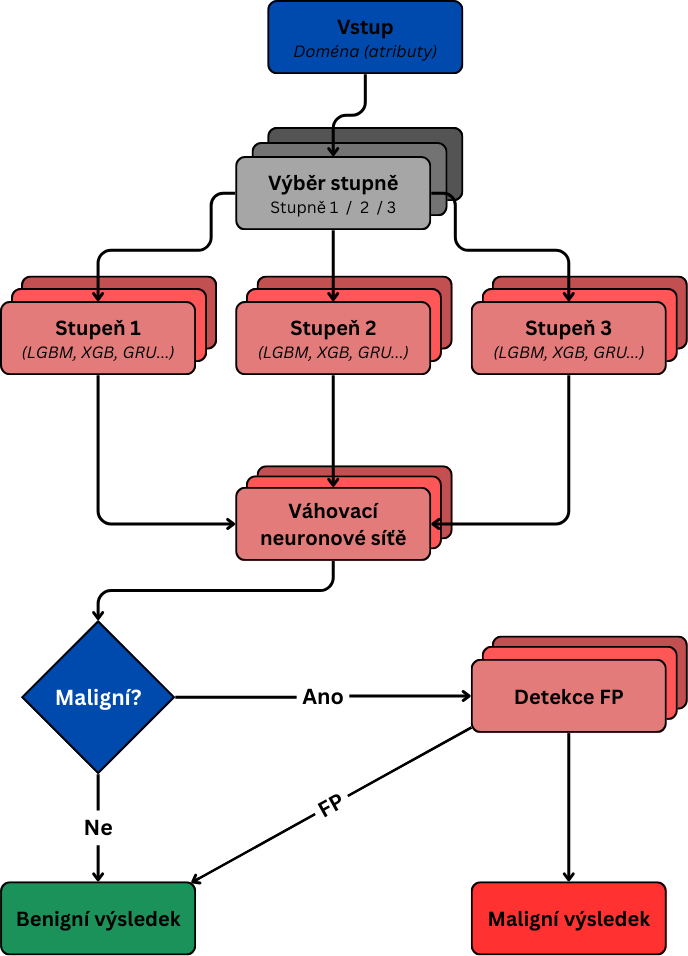
\includegraphics[width=0.8\textwidth]{obrazky-figures/pipeline_final.png}
    \caption{Schéma výsledné klasifikační pipeline}
    \label{fig:classification_pipeline_ensemble}
\end{figure}

\subsection{Mechanismus výběru vhodného stupně}

Při klasifikaci nové domény pipeline nejprve analyzuje dostupné příznaky. Na základě jejich počtu a typu je automaticky vybrán nejvhodnější stupeň (\textit{stage}). Pokud není možné využít model vyššího stupně, pipeline degraduje rozhodování na nižší stupeň.

Výběr stupně je realizován zaokrouhlováním podle počtu dostupných příznaků tak, aby bylo možné použít model optimalizovaný pro danou situaci.

\subsection{Paralelní klasifikace pomocí více modelů}

Pro každý stupeň jsou k~dispozici různé modely (např. XGBoost, Feedforward NN, CNN). Klasifikace probíhá následovně:

\begin{enumerate}
    \item Vyberou se všechny modely odpovídající zvolenému stupni.
    \item Každý model samostatně předpoví pravděpodobnost malignity.
    \item Výsledky jsou agregovány — Metody váhování výstupů jednotlivých modelů jsou rozebrány v~sekci \ref{sec:model_weighting} níže. 
\end{enumerate}

Tento přístup umožňuje kombinovat silné stránky různých modelů a zvyšuje robustnost výsledné predikce.

\subsection{Výhody zvoleného přístupu}

Navržená pipeline přináší následující výhody:

\begin{itemize}
    \item \textbf{Adaptivita:} Funkčnost i při neúplných datech díky dynamickému výběru stupně.
    \item \textbf{Robustnost:} Snížení rizika chybných klasifikací díky kombinovanému přístupu.
    \item \textbf{Flexibilita:} Možnost snadného rozšíření o~nové modely a strategie agregace.
    \item \textbf{Modularita:} Jasné oddělení jednotlivých komponent (výběr stupně, modely, agregace).
\end{itemize}

Díky této koncepci je pipeline vhodná jak pro akademické experimenty, tak pro nasazení v~reálném prostředí s~proměnlivou kvalitou vstupních dat.

\section{Váhování ve výsledné pipeline}
\label{sec:model_weighting}

Při paralelní klasifikaci pomocí více modelů v~rámci jednotlivých stupňů (\textit{stages}) vzniká potřeba vhodně agregovat jejich parciální výstupy. Cílem je získat spolehlivější a robustnější odhad pravděpodobnosti malignity každé domény. V~této sekci popisujeme několik strategií váhování a agregace rozhodnutí modelů, které byly zvažovány nebo implementovány v~rámci této práce.

\subsection{Výběr nejlepšího modelu}

Nejjednodušší přístup spočívá ve využití výstupu jediného modelu, který dosahuje nejlepších výsledků v~rámci validační sady. Tento model je pak považován za reprezentativní pro daný stupeň klasifikace.

\begin{itemize}
    \item \textbf{Výhody:} Nízká výpočetní náročnost, snadná interpretace.
    \item \textbf{Nevýhody:} Ztráta potenciálu ensemble přístupu; náchylnost k~přeučení a variabilitě výkonu při změně dat.
\end{itemize}

\subsection{Nevážený aritmetický průměr výstupů}

Každý model generuje pravděpodobnostní výstup (např. pravděpodobnost, že doména je maligní). Tyto hodnoty se následně zprůměrují a výsledná hodnota slouží jako vstup pro rozhodovací práh.

\[
P_{\text{avg}} = \frac{1}{N} \sum_{i=1}^{N} P_i
\]

kde $P_i$ je výstup $i$-tého modelu a $N$ je počet modelů.

\begin{itemize}
    \item \textbf{Výhody:} Robustní vůči extrémním hodnotám jednoho modelu, jednoduchá implementace.
    \item \textbf{Nevýhody:} Předpokládá stejnou spolehlivost všech modelů.
\end{itemize}

\subsection{Vážený průměr dle výkonnosti modelů}

Modelům jsou přiřazeny váhy $w_i$ na základě jejich validační výkonnosti (např. skóre F1, AUC). Výstupy jsou poté agregovány jako vážený průměr:

\[
P_{\text{weighted}} = \frac{\sum_{i=1}^{N} w_i \cdot P_i}{\sum_{i=1}^{N} w_i}
\]

\begin{itemize}
    \item \textbf{Výhody:} Reflektuje rozdíly v~kvalitě modelů, zvyšuje důraz na spolehlivější prediktory.
    \item \textbf{Nevýhody:} Nutnost udržovat a aktualizovat váhy při každém tréninku.
\end{itemize}

\subsection{Rozhodovací metamodel (meta-klasifikátor)}

Další možností je použití metamodelu, který se učí na výstupech základních modelů. Každý model poskytuje vstupní znak a metamodel (např. logistická regrese, rozhodovací strom) učí optimální váhování a rozhodovací pravidla.

\begin{itemize}
    \item \textbf{Výhody:} Možnost modelovat nelineární vztahy mezi výstupy modelů, adaptivita vůči korelaci mezi modely.
    \item \textbf{Nevýhody:} Vyšší složitost, riziko přeučení, potřeba separátní validační množiny pro trénink metamodelu.
\end{itemize}

\subsection{Většinové hlasování}

Při použití binárních rozhodnutí (např. výstup $P_i > 0{,}5$) je výsledná predikce určena většinou hlasů modelů.

\[
\hat{y} = \text{mode} \left( \mathbb{I}[P_i > \theta] \right)
\]

kde $\mathbb{I}$ je indikátorová funkce a $\theta$ rozhodovací práh (typicky 0{,}5).

\begin{itemize}
    \item \textbf{Výhody:} Vhodné pro situace, kdy je požadována interpretovatelná binární volba.
    \item \textbf{Nevýhody:} Ignoruje nuance pravděpodobností, nevhodné při různé kalibraci modelů.
\end{itemize}

\subsection{Bayesovská agregace}

V~teoretickém rámci lze každý model považovat za samostatný zdroj podmíněné pravděpodobnosti. Kombinace modelů pak může být řešena pomocí Bayesova pravidla nebo jeho aproximací (např. pomocí Naivního Bayese nad výstupy). \cite{bai2015bayesian}

\begin{itemize}
    \item \textbf{Výhody:} Formální pravděpodobnostní rámec, možnost inkorporace apriorních znalostí.
    \item \textbf{Nevýhody:} Obtížná aplikace bez přesné znalosti závislostí mezi modely.
\end{itemize}





\subsection{Souhrn}

Výběr strategie váhování závisí na konkrétních požadavcích systému — zda má být preferována interpretovatelnost, přesnost, robustnost nebo výpočetní efektivita. V~této práci byl primárně využit aritmetický průměr a dále testován vážený průměr dle výkonnosti modelů. Tyto přístupy poskytly dobrý kompromis mezi přesností a jednoduchostí implementace, zejména v~kontextu reálného nasazení s~omezenými výpočetními prostředky.

Přehled vhodnosti jednotlivých strategií ve vztahu k~různým systémovým prioritám shrnuje tabulka~\ref{tab:agg_strategies_compact}.

\begin{table}[H]
\centering
\renewcommand{\arraystretch}{1.1}
\begin{tabular}{|l|c|c|c|c|c|}
\hline
\textbf{Metoda} & \textbf{Složit.} & \textbf{Robust.} & \textbf{Přesn.} & \textbf{Interp.} & \textbf{Adapt.} \\
\hline
Nejlepší model         & + & – & – & + & – \\
Nevážený průměr        & + & + & + & + & – \\
Vážený průměr          & o~& + & + & o~& o~\\
Metamodel              & – & + & + & – & + \\
Hlasování              & + & o~& – & + & – \\
Bayes. agregace        & – & + & o~& o~& o~\\
\hline
\end{tabular}
\caption{Vhodnost váhovacích strategií pro různé požadavky systému.}
\label{tab:agg_strategies_compact}
\end{table}

\vspace{1mm}
\noindent\textbf{Legenda:} + vhodné, o~částečně vhodné, – nevhodné. Sloupce: Složitost implementace, robustnost vůči chybám modelů, predikční přesnost, interpretovatelnost výsledku, adaptabilita na měnící se podmínky.





\section{Rozhodovací neuronová síť (meta-klasifikátor)}

Aby bylo možné efektivně kombinovat výstupy různých modelů zapojených do klasifikační pipeline, byla navržena a implementována specializovaná rozhodovací neuronová síť. Rozhodnutí o~implementaci váhovací sítě vychází z~měření v~sekci \ref{res:aggregation_results}.

Tato neuronová síť slouží jako meta-klasifikátor, který se učí na základě výstupů jednotlivých klasifikátorů a dokáže tak vytvořit finální rozhodnutí s~vyšší přesností a robustností.

\subsection{Motivace a účel}
Ensemble přístup zvyšuje spolehlivost predikce kombinací několika modelů. Nicméně jednoduché metody jako vážený průměr nemusí vždy efektivně zohlednit vzájemné korelace nebo specifické vzory v~chování jednotlivých klasifikátorů. Proto byla implementována neuronová síť, která se učí optimální váhování výstupů modelů a dokáže detekovat i složité nelineární vztahy mezi nimi.

\subsection{Vstupy do metamodelu}
Model přijímá jako vstup vektor pravděpodobnostních skóre jednotlivých klasifikátorů odpovídajících zvolenému klasifikačnímu stupni (např. výstupy modelů XGBoost, FFNN, CNN pro Stage 3). Vstupy mohou dále zahrnovat další metadata, například:
\begin{itemize}
\item Počet příznaků dostupných pro danou doménu
\item Výsledky TLS klasifikátoru
\item Entropii vstupního vektoru
\end{itemize}

\subsection{Architektura rozhodovací neuronové sítě}
Model je implementován jako plně propojená neuronová síť s~následující architekturou:

\begin{verbatim}
Sequential([
Dense(32, input_dim=n_features, activation="relu"),
Dropout(0.2),
Dense(16, activation="relu"),
Dense(1, activation="sigmoid"),
])
\end{verbatim}

Model je trénován s~použitím binární entropie jako ztrátové funkce a optimalizátoru Adam (learning rate 0.001). Trénování probíhá s~validačním dělením dat 70/30 a využitím early stopping pro prevenci přeučení.

\subsection{Výhody a výsledky}
Rozhodovací neuronová síť přináší vyšší flexibilitu a schopnost zohlednit komplexní interakce mezi modely. V~porovnání s~jednoduchými váhovacími metodami (aritmetický průměr, vážený průměr) dosahovala mírně vyšší skóre F1 a lépe odolávala výkyvům v~kvalitě výstupů jednotlivých modelů.

Z~hlediska výkonu je model dostatečně rychlý pro online inferenci v~provozním prostředí a lze jej dále rozšířit o~více vstupních znaků, např. entropii predikcí nebo volatilitu předchozích rozhodnutí.

Model byl validován jako součást hlavní pipeline a jeho přínos byl analyzován v~kapitole \ref{experiments:eval}, sekce \ref{res:aggregation_results}.

\subsection*{Poznámka k~implementaci a zařazení}
Rozhodovací neuronová síť byla implementována jako jedna z~několika strategií váhování výstupů modelů (viz kapitola~\ref{sec:model_weighting}). Z~pohledu přesnosti a robustnosti se ukázala jako nejvhodnější varianta, a proto byla využita jako finální agregátor v~navržené pipeline. Implementace využívá framework TensorFlow/Keras a plně propojenou architekturu popsanou výše. Detailní vyhodnocení je uvedeno v~sekci~\ref{res:aggregation_results}.






\section{Detekce falešně pozitivních vzorků}
\label{sec:false_positive_detection}

Při provozním nasazení systému \textit{DomainRadar} je klíčové minimalizovat počet falešně pozitivních detekcí (FP), tedy situací, kdy benigní doména byla chybně označena jako maligní. I~při vysoké přesnosti klasifikátorů mohou i jednotky procent FP znamenat stovky nebo tisíce chybných alertů za minutu — vzhledem k~tomu, že systém zpracovává statisíce domén každou minutu. Takové množství varování je pro lidské operátory neudržitelné a vede k~ignorování detekcí nebo přetížení bezpečnostních týmů. 

Z~tohoto důvodu byla do pipeline integrována specializovaná vrstva pro \textbf{dodatečnou identifikaci falešně pozitivních výsledků}. Ta slouží jako pojistka nad hlavním rozhodovacím mechanismem a umožňuje snížit falešně pozitivní míru bez výrazného dopadu na míru detekce hrozeb (TPR).

\subsection{Motivace a princip fungování}

Zvolený přístup využívá hlavní výstup klasifikace (po agregaci napříč modely, viz \ref{sec:model_weighting}) a na jeho základě vytváří \textbf{trénovací sadu pro detekci falešně pozitivních výsledků}. Konkrétně se extrahují případy, kdy byla doména klasifikována jako maligní, ale její skutečný štítek je benigní. Tyto případy tvoří pozitivní třídu pro trénink doplňkového modelu (tzv. \textit{false-positive detector}, FPD), jehož cílem je naučit se jemné rozdíly mezi pravými hrozbami a chybně označenými benigními doménami.

Model FPD je trénován nezávisle na hlavních klasifikátorech, čímž je zajištěna modularita a možnost jeho samostatné optimalizace. Trénink probíhá paralelně s~validací hlavního ensemble modelu.

\subsection{Integrace rozhodnutí do pipeline}

Kombinace hlavního klasifikátoru a FPD je řešena dvouvrstvě:
\begin{enumerate}
    \item Nejprve dojde k~rozhodnutí hlavním klasifikátorem — typicky váhovanou agregací více modelů daného stupně.
    \item Pokud výstup indikuje, že doména je maligní, je výsledek ověřen modelem FPD.
    \item Pokud FPD predikuje, že se s~vysokou pravděpodobností jedná o~falešně pozitivní detekci, je výstup přehodnocen na \textbf{benigní}.
\end{enumerate}

Tento mechanismus zajišťuje, že FP mají ještě jednu šanci být identifikovány před generováním finálního alertu.

\subsection{Architektura a implementace modelu FPD}
\label{sec:fpd_architecture}

Pro detekci falešně pozitivních vzorků je použita \textbf{plně propojena neuronova síť (feedforward neural network)}, implementovaný v~TensorFlow/Keras. Vstupy do modelu tvoří charakteristiky domén, které byly hlavním klasifikátorem označeny jako maligní, včetně embedovaných atributů a metadat.

\paragraph{Architektura modelu:}
\begin{verbatim}
Sequential([
    Dense(64, input_dim=X_train.shape[1], activation="relu"),
    Dropout(0.2),
    Dense(32, activation="relu"),
    Dropout(0.1),
    Dense(1, activation="sigmoid"),
])
\end{verbatim}

Model je optimalizován pomocí algoritmu Adam s~learning rate 0{,}001 a trénován na binární entropii (\texttt{binary\_crossentropy}). Pro zvýšení robustnosti a zamezení přeučení je použito \textbf{early stopping} na validační ztrátě s~patiencí 5 epoch.

\paragraph{Zpracování vstupů:} Vstupy do modelu jsou normalizovány pomocí standardního škálování (\texttt{StandardScaler}) trénovaného výhradně na trénovacích datech. Tento scaler je uložen spolu s~modelem a použit i při inferenci, čímž se zajišťuje konzistence během nasazení.


% \section{Architektura systému}
% 1. Nejprve se rozhodne kolik dat k dané doméně je. Počet příznaků se zaokrouhlí a ořeže na nejbližší nižší stupeň. 

% Doména je klasifikována klasifikátory pro danou fázi. V případně fáze 2 a 3 je použit i klasifikátor TLS a CNN. 

% Tyto výsledky společně s meta daty jdou to meta klasifikátoru, který provede predikci výsledku. V případně pozitivního výsledku jde celá doména do FPD klasifikátoru, který detekuje případné falešně pozitivní výsledky. 

% Vše je naznačeno na grafu \ref{fig:classification_pipeline_ensemble}









\chapter{Vyhodnocení a experimenty}
\label{experiments:eval}\label{chapter:9}

V~této kapitole jsou prezentovány výsledky testování a porovnání jednotlivých modelů na různých datových sadách. Cílem je vyhodnotit výkonnost navržených klasifikátorů v~rámci vícestupňové klasifikace domén a posoudit jejich vhodnost pro nasazení v~reálném provozu. 

Všechna měření byla provedena na základě \textbf{validační sady dat}, která vznikla rozdělením kompletní datové sady uvedené v~kapitole~\ref{chapter:5} (70~\% trénovací data, 30~\% validační data). Pro zajištění stability a spolehlivosti výsledků byly modely trénovány a vyhodnocovány v~rámci \textbf{10 opakovaných běhů} s~různým náhodným počátečním stavem. Výsledné metriky jsou uváděny jako průměrné hodnoty včetně směrodatné odchylky. Vyhodnocení je rozděleno do několika částí:
\begin{itemize}
    \item Nejprve jsou uvedeny souhrnné výsledky modelů pro klasifikační fáze 1 a 2. Tyto fáze reprezentují situace, kdy není k~dispozici kompletní sada příznaků (např. při detekci nových domén v~reálném čase).
    \item Následuje podrobné vyhodnocení klasifikační fáze 3 (plná data), kde jsou jednotlivé modely analyzovány detailně – včetně matic záměn, diskuse nad chybami a srovnání jejich chování.
    \item V~závěru kapitoly je vyhodnocena celá klasifikační pipeline jako celek, včetně strategie váhování výstupů modelů a využití modulu pro detekci falešně pozitivních vzorků (FPD).
\end{itemize}

\section{Přehled výsledků}

Tabulka~\ref{tab:summary_phishing_stages} shrnuje dosažené výsledky jednotlivých modelů napříč třemi klasifikačními fázemi (\textit{Stage 1} – pouze lexikální příznaky, \textit{Stage 2} – síťové příznaky bez obsahu, \textit{Stage 3} – plná datová reprezentace). Pro každý model a fázi jsou uvedeny tři hlavní metriky: přesnost klasifikace (Accuracy), skóre F1 a plocha pod ROC křivkou (ROC AUC). Tučně jsou zvýrazněny nejlepší hodnoty v~rámci dané fáze.

Vzhledem k~výrazné nevyváženosti tříd byla jako klíčová metrika zvolena hodnota F1 skóre, která lépe odráží rovnováhu mezi přesností a úplností při klasifikaci menšinové třídy. Přesnost (Accuracy) a plocha pod křivkou (ROC AUC) poskytují doplňkový pohled na výkonnost modelu napříč různými rozhodovacími prahy.


¨
\begin{table}[H]
\centering
\small
\begin{tabular}{|l|l|c|c|c|}
\hline
\textbf{model} & \textbf{fáze} & \textbf{přesnost} & \textbf{skóre F1} & \textbf{ROC AUC} \\
\hline
XGBoost  & Stage 1 & 0.9651          & 0.8884          & 0.9829          \\
LightGBM & Stage 1 & 0.9529          & 0.8446          & 0.9706          \\
FFNN     & Stage 1 & \textbf{0.9676} & \textbf{0.8942} & \textbf{0.9838} \\
SVM      & Stage 1 & 0.9630          & 0.8840          & 0.9389          \\
\hline
XGBoost  & Stage 2 & 0.9782           & 0.9328         & 0.9951  \\
LightGBM & Stage 2 & \textbf{0.9880} & \textbf{0.9638} &\textbf{0.9982}         \\
FFNN     & Stage 2 & 0.9801          & 0.9404          & 0.9643          \\
SVM      & Stage 2 & 0.9801          & 0.9801          & 0.9801          \\
\hline
XGBoost  & Stage 3 & \textbf{0.9953} & \textbf{0.9860} & \textbf{0.9996} \\
LightGBM & Stage 3 & 0.9905          & 0.9711          & 0.9987          \\
FFNN     & Stage 3 & 0.9927          & 0.9780          & 0.9857          \\
CNN      & Stage 3 & 0.9546          & 0.9654         & 0.9706             \\
SVM      & Stage 3 & 0.9715          & 0.9691          & 0.9891          \\
\hline
\end{tabular}
\caption{Souhrn klasifikačních metrik (phishing) napříč modely a klasifikačními fázemi. Nejlepší hodnoty pro každou fázi (Accuracy, skóre F1 a ROC AUC) jsou vyznačeny tučně.}
\label{tab:summary_phishing_stages}
\end{table}

\begin{table}[H]
\centering
\small
\begin{tabular}{|l|l|c|c|c|}
\hline
\textbf{model} & \textbf{fáze} & \textbf{přesnost} & \textbf{skóre F1} & \textbf{ROC AUC} \\
\hline
XGBoost  & Stage 1 & 0.9602          & 0.8802          & 0.9815          \\
LightGBM & Stage 1 & 0.9512          & 0.8654          & 0.9743          \\
FFNN     & Stage 1 & \textbf{0.9638} & \textbf{0.8841} & \textbf{0.9831} \\
SVM      & Stage 1 & 0.9584          & 0.8772          & 0.9653          \\
\hline
XGBoost  & Stage 2 & 0.9762          & 0.9501          & 0.9973          \\
LightGBM & Stage 2 & \textbf{0.9902} & \textbf{0.9639} & \textbf{0.9973} \\
FFNN     & Stage 2 & 0.9833          & 0.9467          & 0.9644          \\
SVM      & Stage 2 & 0.9800          & 0.9657          & 0.9884          \\
\hline
XGBoost  & Stage 3 & \textbf{0.9944} & \textbf{0.9744}  & \textbf{0.9994} \\
LightGBM & Stage 3 & 0.9896          & 0.9517          & 0.9984          \\
FFNN     & Stage 3 & 0.9869          & 0.9391          & 0.9585          \\
CNN      & Stage 3 & 0.9546          & 0.7451          & 0.8013          \\
SVM      & Stage 3 & 0.9888          & 0.9657          & 0.9884          \\
\hline
\end{tabular}
\caption{Souhrn klasifikačních metrik (malware) napříč modely a klasifikačními fázemi. Nejlepší hodnoty pro každou fázi (Accuracy, skóre F1 a ROC AUC) jsou vyznačeny tučně.}
\label{tab:summary_malware_stages}
\end{table}

Jak je z~tabulky patrné, výkon modelů se významně zvyšuje s~dostupností bohatších příznaků. Ve fázi 1 dosahuje nejlepšího výsledku model FFNN, v~klasifikační fázi 2 dominuje LightGBM, zatímco ve fázi 3 (plná data) dosahuje nejlepší přesnosti XGBoost. To potvrzuje vhodnost kombinace více modelů při nasazení do produkčního prostředí, kde jsou dostupné různé úrovně informací o~doméně.



\section{SVM}
Support Vector Machine (SVM) patří mezi tradiční metody klasifikace, které se uplatňují zejména při menším množství příznaků. Model se ukázal jako stabilní napříč všemi fázemi, přičemž v~klasifikační fázi~2 vykazuje velmi dobré skóre F1  i schopnost generalizace. Jeho výkon ve fázi~1 byl solidní, avšak nepřekonal neuronové architektury. Model je vhodný pro referenční porovnání a případy, kde je důležitá vysoká úplnost a predikovatelný výstup.

\subsection{Výsledky klasifikace}
Výsledky klasifikace dosažené pomocí SVM modelu jsou pro phishingové a malware domény uvedeny v~tabulce \ref{tab:svm_malware_phishing_results}.

\begin{table}[H]
\centering
\begin{tabular}{|l|c|c|}
\hline
\textbf{Metrika} & \textbf{Phishing} & \textbf{Malware} \\
\hline
Přesnost klasifikace (Accuracy)     & \texttt{0.9715 ± 2.1e-04} & \texttt{0.9888 ± 1.7e-04} \\
Přesnost pozitivní třídy (Precision)    & \texttt{0.9902 ± 2.3e-07} & \texttt{0.9692 ± 2.6e-07} \\
Úplnost (Recall)        & \texttt{0.9671 ± 3.2e-07} & \texttt{0.9459 ± 3.0e-07} \\
skóre F1                & \texttt{0.9691 ± 2.7e-07} & \texttt{0.9657 ± 2.4e-07} \\
ROC AUC                 & \texttt{0.9891 ± 6.1e-06} & \texttt{0.9884 ± 5.4e-06} \\
\hline
\end{tabular}
\caption{Metriky modelu SVM pro phishingové a malware domény (10 běhů)}
\label{tab:svm_malware_phishing_results}
\end{table}

\subsection{Analýza matice záměn}

Úspěšnost klasifikace pomocí SVM je dále ilustrována pomocí matic záměn pro malware domény a phishing domény. 

\begin{figure}[H]
    \centering
    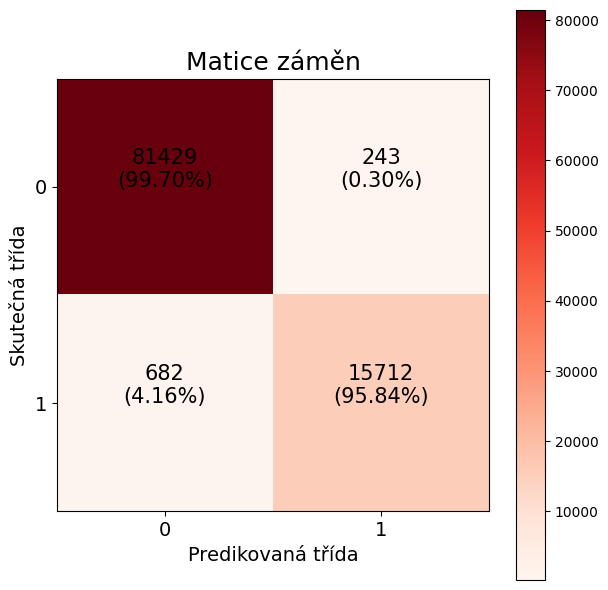
\includegraphics[width=0.8\textwidth]{obrazky-figures/svm_stage_3_phishing_v1.1_confusion_matrix.png}
    \caption{Matice záměn modelu SVM pro phishingové domény}
    \label{fig:svm_conf_matrix_phishing}
\end{figure}

\begin{figure}[H]
    \centering
    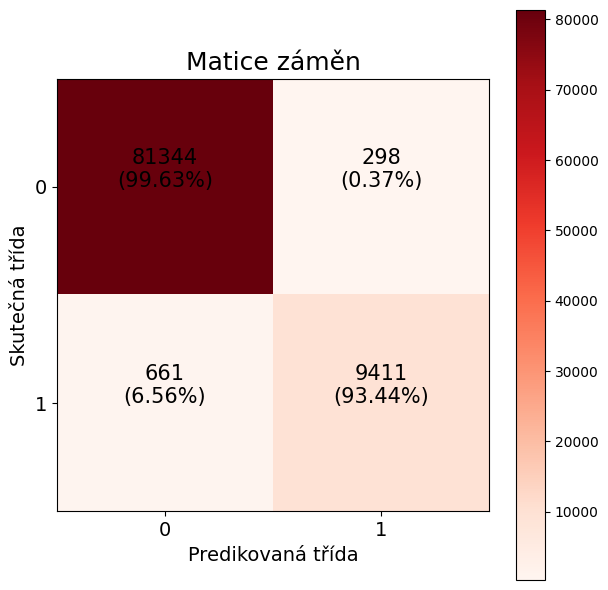
\includegraphics[width=0.8\textwidth]{obrazky-figures/svm_stage_3_malware_v1.1_confusion_matrix.png}
    \caption{Matice záměn modelu SVM pro malware domény}
    \label{fig:svm_conf_matrix_malware}
\end{figure}

\subsection{Shrnutí výkonu modelu}

Model SVM dosáhl velmi dobrých výsledků při detekci maligních domén, přičemž:
\begin{itemize}
    \item Přesnost klasifikace dosáhla hodnoty 98\%.
    \item Recall pro třídu maligních domén (1) dosáhl 94,97\%, což ukazuje na nízký počet falešně negativních případů.
    \item Model vykazuje vyšší míru falešně pozitivních predikcí ve srovnání s~modely XGBoost a LightGBM.
\end{itemize}

I~přes vyšší hodnotu FPR ukazuje SVM vysoký potenciál při detekci hrozeb v~případech, kde je požadována vysoká úplnost a robustnost.




\section{LGBM}\label{res:lgbm}
LightGBM je výkonný gradient boosting framework optimalizovaný pro rychlost a paměťovou efektivitu. Ve fázi~1 mírně zaostává za jinými modely, zejména v~oblasti recall a skóre F1. Naopak ve fázi~2 již dosahuje velmi konkurenceschopných výsledků a je vhodný pro reálné nasazení v~prostředí s~omezenými výpočetními prostředky. Výhodou je vysoká rychlost tréninku a predikce při zachování velmi dobré přesnosti.


\subsection{Výsledky klasifikace}

Modely byly testovány na samostatné testovací sadě domén. Dosažené metriky pro detekci phishingových a malware domén pomocí modelu LightGBM jsou shrnuty v~tabulce \ref{tab:lgbm_malware_phishing_results} níže:

\begin{table}[H]
\centering
\begin{tabular}{|l|c|c|}
\hline
\textbf{Metrika} & \textbf{Phishing} & \textbf{Malware} \\
\hline
Přesnost klasifikace (Accuracy) & \texttt{0.9905 ± 1.1e-04} & \texttt{0.9896 ± 1.3e-04} \\
Přesnost pozitivní třídy (Precision) & \texttt{0.9848 ± 2.5e-07} & \texttt{0.9692 ± 3.0e-07} \\
Úplnost (Recall) & \texttt{0.9578 ± 3.1e-07} & \texttt{0.9349 ± 2.8e-07} \\
skóre F1 & \texttt{0.9711 ± 1.8e-07} & \texttt{0.9517 ± 2.1e-07} \\
ROC AUC & \texttt{0.9987 ± 5.5e-06} & \texttt{0.9984 ± 4.8e-06} \\
\hline
\end{tabular}
\caption{Metriky modelu LightGBM (10 běhů)}
\label{tab:lgbm_malware_phishing_results}
\end{table}

Z~tabulky je patrné, že model LightGBM vykazuje velmi dobrý výkon při detekci jak phishingových, tak malware domén. Model dosáhl vyšší přesnosti u~phishingových domén, což je patrné zejména na vyšší hodnotě přesnosti, skóre F1 i nižší falešné pozitivní míře (FPR). Výsledky naznačují dobrou schopnost modelu generalizovat na neznámá data s~minimálním počtem chyb v~predikci.

\subsection{Analýza matice záměn}

Výkonnost modelu LightGBM je dále ilustrována pomocí matic záměn \ref{fig:lgbm_conf_matrix_phishing} a \ref{fig:lgbm_conf_matrix_malware} níže.

\begin{figure}[H]
    \centering
    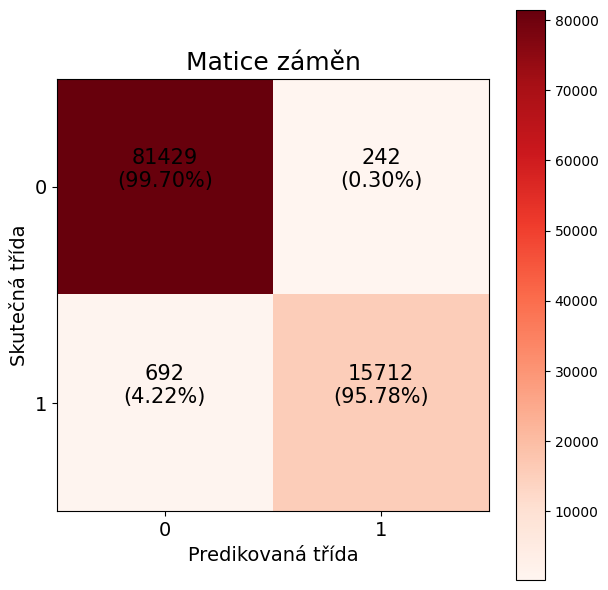
\includegraphics[width=0.8\textwidth]{obrazky-figures/Lgbm_stage_3_phishing_v1.1_confusion_matrix.png}
    \caption{Matice záměn modelu LightGBM pro phishingové domény}
    \label{fig:lgbm_conf_matrix_phishing}
\end{figure}

\begin{figure}[H]
    \centering
    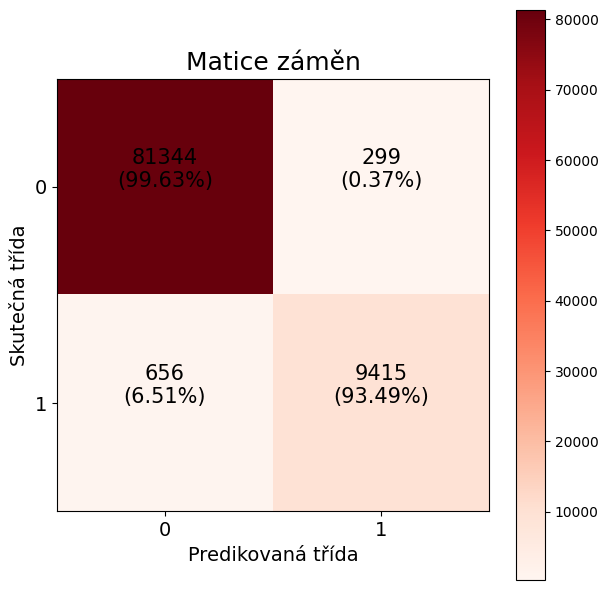
\includegraphics[width=0.8\textwidth]{obrazky-figures/Lgbm_stage_3_malware_v1.1_confusion_matrix.png}
    \caption{Matice záměn modelu LightGBM pro malware domény}
    \label{fig:lgbm_conf_matrix_malware}
\end{figure}

\subsection{Shrnutí výkonu modelu}

Model LightGBM potvrdil svou vysokou efektivitu při klasifikaci domén, přičemž:
\begin{itemize}
    \item Dosažené metriky byly srovnatelné s~modelem XGBoost.
    \item Trénink a predikce byly mírně rychlejší díky optimalizované implementaci.
    \item LightGBM vykazuje dobrou generalizaci na neznámých datech.
\end{itemize}

Tento model je vhodný pro nasazení v~reálných podmínkách s~omezenými výpočetními zdroji.




\section{XGBoost}\label{res:xgb}
Model XGBoost je jedním z~nejvýkonnějších stromových modelů současnosti a jeho výsledky to potvrzují napříč všemi fázemi. Již ve fázi~1 dosahuje výborné přesnosti i skóre F1, ve fázi~3 pak dominuje všem ostatním modelům ve všech hlavních metrikách. Vysoká robustnost a interpretovatelnost výstupů z~něj činí velmi silného kandidáta pro reálné nasazení.


\subsection{Výsledky klasifikace}

Model byl testován na samostatné testovací sadě domén. Dosažené metriky pro detekci malware a phishingových domén pomocí modelu XGBoost jsou shrnuty v~tabulce \ref{tab:xgboost_malware_phishing_results}.

\begin{table}[h!]
\centering
\begin{tabular}{|l|c|c|}
\hline
\textbf{Metrika} & \textbf{Malware} & \textbf{Phishing} \\
\hline
Přesnost klasifikace (Accuracy) & \texttt{0.9944 ± 1.2e-04} & \texttt{0.9953 ± 1.0e-04} \\
Přesnost pozitivní třídy (Precision) & \texttt{0.9844 ± 2.1e-07} & \texttt{0.9928 ± 1.9e-07} \\
Úplnost (Recall) & \texttt{0.9646 ± 2.8e-07} & \texttt{0.9792 ± 2.3e-07} \\
skóre F1 & \texttt{0.9744 ± 1.9e-07} & \texttt{0.9860 ± 1.6e-07} \\
ROC AUC & \texttt{0.9994 ± 3.1e-06} & \texttt{0.9996 ± 2.7e-06} \\
\hline
\end{tabular}
\caption{Metriky modelu XGBoost (10 běhů)}
\label{tab:xgboost_malware_phishing_results}
\end{table}




Z~tabulky je patrné, že model XGBoost dosahuje vysoké přesnosti v~detekci jak malware, tak phishingových domén. Mírně lepších výsledků bylo dosaženo u~phishingových domén, zejména v~oblasti přesnosti a snížené falešné pozitivní míry.



\subsection{Analýza matice záměn}

Výkon modelu je dále ilustrován pomocí dvou matic záměn (confusion matrix). Pro malware a phishing domény. Matice \ref{fig:xgboost_conf_matrix_malware} a \ref{fig:xgboost_conf_matrix_phishing} znázorňují rozdělení správně a nesprávně klasifikovaných vzorků:.

\begin{figure}[H]
    \centering
    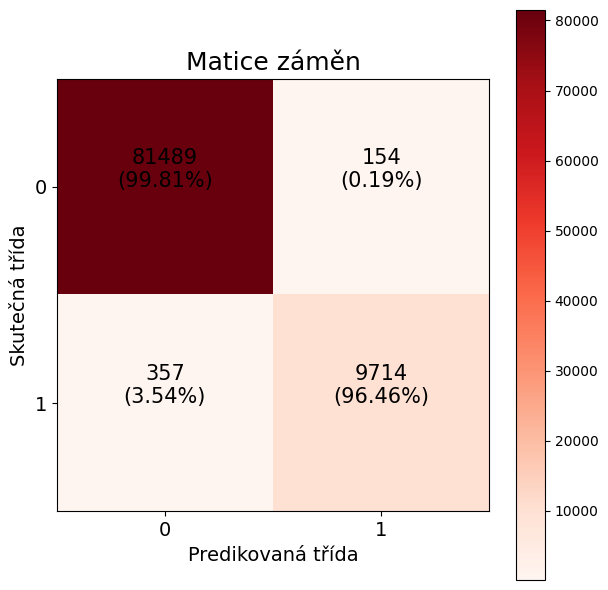
\includegraphics[width=0.8\textwidth]{obrazky-figures/XgBoost_stage_3_malware_v1.1_confusion_matrix.png}
    \caption{Matice záměn modelu XGBoost pro malware domémny}
    \label{fig:xgboost_conf_matrix_malware}
\end{figure}

\begin{figure}[H]
    \centering
    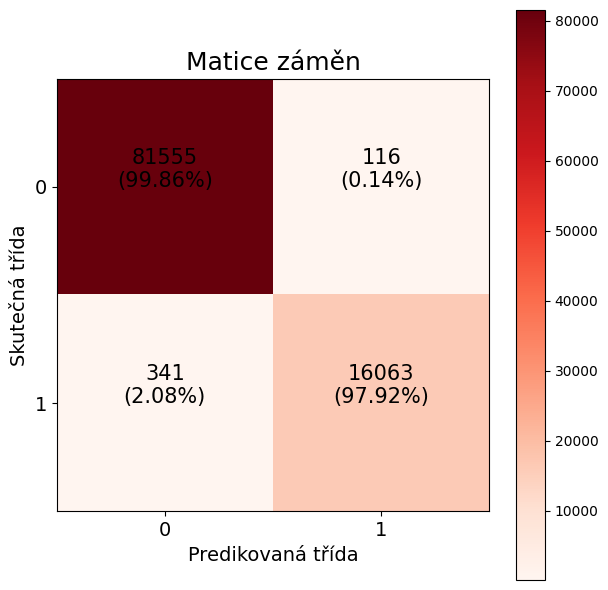
\includegraphics[width=0.8\textwidth]{obrazky-figures/XgBoost_stage_3_phishing_v1.1_confusion_matrix.png}
    \caption{Matice záměn modelu XGBoost pro phishingové domény}
    \label{fig:xgboost_conf_matrix_phishing}
\end{figure}


Z~matice záměn je patrné, že model vykazuje vysokou míru správné klasifikace benigních i maligních domén, s~nízkým počtem falešně pozitivních a falešně negativních vzorků.

\subsection{Shrnutí výkonu modelu}

Model XGBoost prokázal vysokou efektivitu při klasifikaci doménových jmen. Mezi hlavní výhody patří:
\begin{itemize}
    \item Vysoká přesnost a robustnost napříč různými sadami příznaků.
    \item Relativně rychlý trénink a predikce díky efektivnímu využití paměti.
    \item Dobrá interpretovatelnost výsledků díky stromové struktuře modelu.
\end{itemize}

XGBoost se ukázal jako vhodná volba zejména pro případy, kdy jsou k~dispozici kvalitní a dobře strukturované atributy.





\section{Dopředná neuronová síť (FFNN)}\label{res:feedforward}
Plně propojená neuronová síť se ukázala jako překvapivě výkonný model i ve fázi~1, kde předčila ostatní metody. Díky své jednoduchosti a schopnosti adaptovat se na různé typy vstupních dat vykazuje dobrý výkon i ve fázi~2. Její výhodou je rychlá konvergence a možnost využití i při menších datových objemech. Model je vhodný jako základní neuronová architektura pro další experimenty.


\subsection{Výsledky klasifikace}

Model plně propojené neuronové sítě byl testován na stejné testovací sadě jako ostatní klasifikátory. Výsledky klasifikace pro detekci malware a phishingových domén jsou shrnuty v~tabulce \ref{tab:feedforward_results}.

\begin{table}[h!]
\centering
\begin{tabular}{|l|c|c|}
\hline
\textbf{Metrika} & \textbf{Malware} & \textbf{Phishing} \\
\hline
Přesnost klasifikace (Accuracy) & \texttt{0.9869 ± 2.2e-04} & \texttt{0.9927 ± 1.5e-04} \\
Přesnost pozitivní třídy (Precision) & \texttt{0.9567 ± 3.1e-07} & \texttt{0.9807 ± 2.5e-07} \\
Úplnost (Recall) & \texttt{0.9221 ± 3.5e-07} & \texttt{0.9753 ± 2.9e-07} \\
skóre F1 & \texttt{0.9391 ± 2.9e-07} & \texttt{0.9780 ± 2.2e-07} \\
ROC AUC & \texttt{0.9585 ± 8.5e-06} & \texttt{0.9857 ± 5.4e-06} \\
\hline
\end{tabular}
\caption{Metriky modelu dopředné neuronové sítě (10 běhů)}
\label{tab:feedforward_results}
\end{table}

Z~výsledků je patrné, že i jednoduchá architektura plně propojené neuronové sítě může dosáhnout vysoké výkonnosti při klasifikaci domén, přičemž výsledky jsou zvláště přesvědčivé u~phishingových domén.

\subsection{Analýza matice záměn}

Model dosáhl velmi vyváženého poměru mezi TPR a FPR. Vizualizace matic záměn ukazuje detailní rozložení klasifikovaných vzorků:

\begin{figure}[H]
\centering
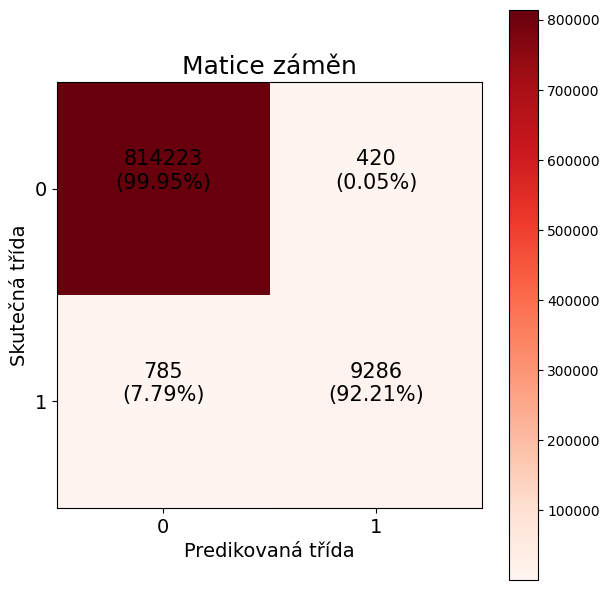
\includegraphics[width=0.8\textwidth]{obrazky-figures/feedforward_stage_3_malware_v1.1_confusion_matrix.png}
\caption{Matice záměn modelu feedforward NN pro malware domény}
\label{fig:ffnn_conf_matrix_malware}
\end{figure}

\begin{figure}[H]
\centering
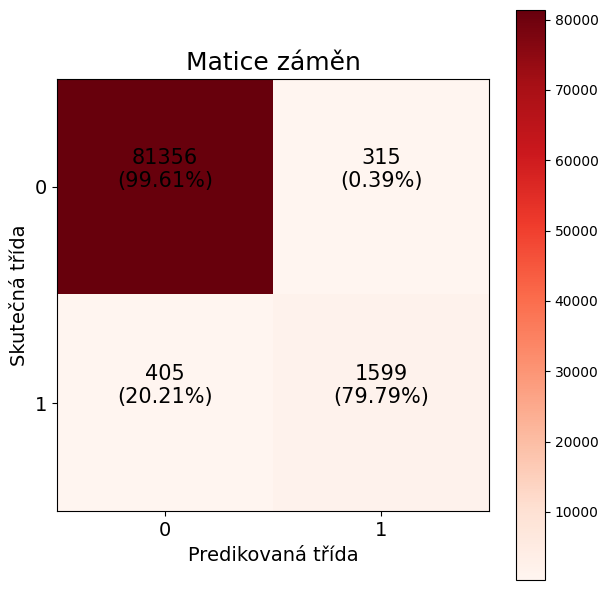
\includegraphics[width=0.8\textwidth]{obrazky-figures/feedforward_stage_3_phishing_v1.1_confusion_matrix.png}
\caption{Matice záměn modelu feedforward NN pro phishingové domény}
\label{fig:ffnn_conf_matrix_phishing}
\end{figure}

Z~matic je zřejmé, že model má vysokou citlivost i specifitu, a to i přes svou relativní jednoduchost ve srovnání s~komplexnějšími architekturami.

\subsection{Shrnutí výkonu modelu}

Plně propojená neuronová síť představuje výkonnou a flexibilní architekturu vhodnou pro doménovou klasifikaci, pokud jsou vstupní data vhodně reprezentována. Mezi hlavní výhody patří:
\begin{itemize}
    \item Snadná implementace a rychlá konvergence.
    \item Robustní výkonnost napříč různými typy domén.
    \item Dobrá přenositelnost na různé datové reprezentace bez nutnosti specifické transformace (např. 2D nebo sekvenční vstupy).
\end{itemize}

Tento model lze doporučit jako referenční základ pro další experimenty s~hlubokým učením, případně jako komponentu složeného klasifikátoru.



\section{Konvoluční neuronová síť (CNN)}\label{res:cnn}

Konvoluční neuronové sítě (CNN) jsou navrženy pro efektivní zpracování strukturovaných dat s~lokálními vzory. Ačkoliv byly původně vyvinuty pro práci s~obrazovými daty, v~této práci se ukazují jako velmi vhodné i pro analýzu doménových jmen. Právě domény často obsahují opakující se struktury (např. fragmenty jako ``login'', ``secure'' nebo ``paypal''), které mohou být efektivně zachyceny konvolučními filtry.

V~této práci byla navržena hlubší CNN architektura obsahující tři konvoluční bloky, každé s~normalizací, aktivační funkcí a poolingem, následované dvěma hustými vrstvami s~dropoutem. Model byl testován ve všech třech klasifikačních fázích. Výsledky ukazují, že výkon CNN výrazně roste s~rozsahem vstupních příznaků – ve fázi~3 dosahuje jednoho z~nejvyšších skóre F1 napříč všemi modely. To naznačuje, že při dalším rozšíření dat nebo příznakové reprezentace by CNN mohla překonat i nejvýkonnější stromové modely jako XGBoost.

\subsection{Výsledky klasifikace}

Model CNN byl vyhodnocen na samostatné testovací sadě analogicky s~ostatními modely. Tabulka~\ref{tab:cnn_malware_phishing_results} shrnuje dosažené metriky pro detekci phishingových i malware domén.

\begin{table}[H]
\centering
\begin{tabular}{|l|c|c|}
\hline
\textbf{Metrika} & \textbf{Malware} & \textbf{Phishing} \\
\hline
Přesnost klasifikace (Accuracy)        & \texttt{0.9546 ± 1.1e-04} & \texttt{0.9887 ± 1.0e-04} \\
Přesnost pozitivní třídy (Precision)       & \texttt{0.9702 ± 5.9e-05} & \texttt{0.9884 ± 1.0e-04} \\
Úplnost (Recall )           & \texttt{0.6048 ± 6.8e-05} & \texttt{0.9435 ± 1.4e-04} \\
skóre F1                   & \texttt{0.7451 ± 5.5e-05} & \texttt{0.9654 ± 1.4e-04} \\
ROC AUC                    & \texttt{0.8013 ± 7.7e-05} & \texttt{0.9706 ± 1.1e-04} \\
\hline
\end{tabular}
\caption{Metriky modelu konvoluční neuronové sítě (CNN) pro malware a phishing domény (10 běhů)}
\label{tab:cnn_malware_phishing_results}
\end{table}

Z~výsledků je patrné, že CNN si velmi dobře poradí s~detekcí phishingových domén. Model vykazuje výborný poměr mezi přesností a úplností a dosahuje jednoho z~nejvyšších skóre F1  ve fázi~3. Zároveň si zachovává mimořádně nízký počet falešně pozitivních detekcí, což je zásadní pro praktické nasazení v~produkčním prostředí.

Naopak u~detekce malware domén model selhává v~oblasti úplnosti (recall), což znamená, že mu uniká velká část škodlivých případů. Přesto však i v~této úloze vykazuje velmi nízkou míru falešně pozitivních výsledků (FP), což může být cenné v~kombinovaných systémech, kde se CNN využívá jako precizní filtr.

\subsection{Analýza matice záměn}

\begin{figure}[H]
    \centering
    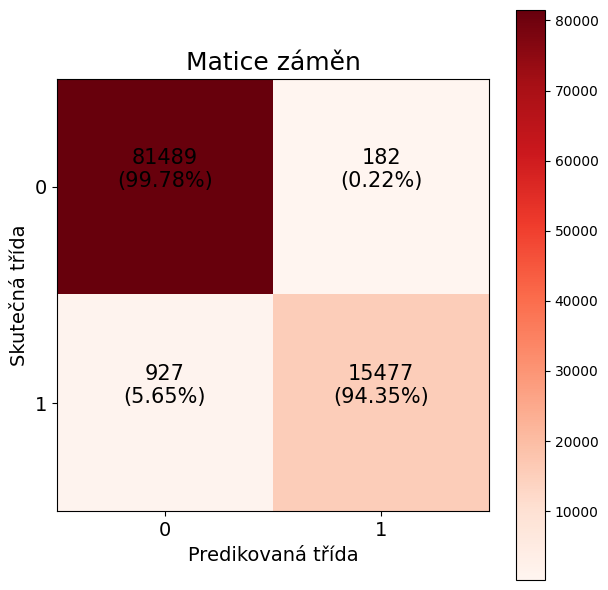
\includegraphics[width=0.8\textwidth]{obrazky-figures/cnn_stage_3_phishing_v1.1_confusion_matrix.png}
    \caption{Matice záměn modelu CNN pro phishingové domény}
    \label{fig:cnn_conf_matrix_phishing}
\end{figure}

\begin{figure}[H]
    \centering
    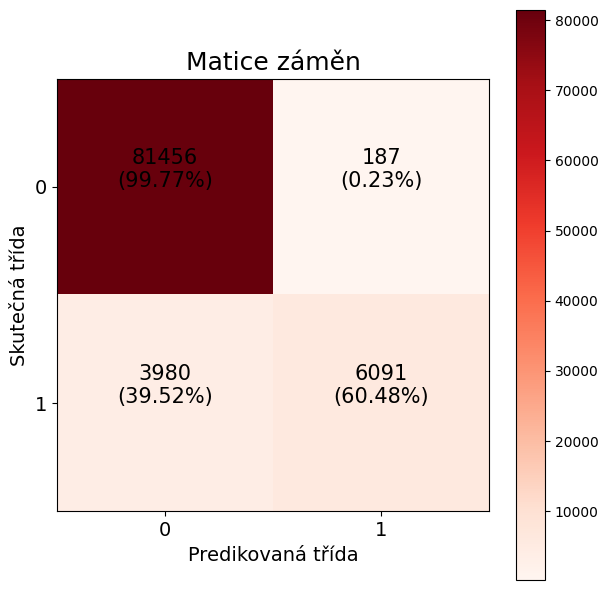
\includegraphics[width=0.8\textwidth]{obrazky-figures/cnn_stage_3_malware_v1.1_confusion_matrix.png}
    \caption{Matice záměn modelu CNN pro malware domény}
    \label{fig:cnn_conf_matrix_malware}
\end{figure}

\subsection{Shrnutí výkonu modelu}

Model CNN ukazuje vysoký potenciál pro detekci phishingových domén a je konkurenceschopný vůči nejlepším stromovým i neuronovým architekturám. Mezi jeho klíčové charakteristiky patří:

\begin{itemize}
    \item Vysoké skóre F1 a preciznost pro phishing, mimořádně nízká falešná pozitivita.
    \item Nízký recall pro malware domény, což omezuje jeho samostatnou použitelnost v~této oblasti.
    \item Výrazné zlepšování výkonu se zvětšujícím se vstupním vektorem – potenciál pro nasazení nad rozsáhlejšími daty.
    \item Vhodný kandidát pro kombinované přístupy (např. ensemble, dvojstupňová detekce).
\end{itemize}

Celkově lze CNN považovat za robustní a precizní model pro detekci phishingu s~možností dalšího vylepšení pro malware klasifikaci prostřednictvím ladění architektury nebo rozšíření trénovacích dat.










\section{FPD – Detekce falešně pozitivních vzorků}
\label{sec:fpd}

Součástí navržené klasifikační pipeline je i komponenta pro dodatečné zpracování výstupů modelu – \textbf{False Positive Detector (FPD)}. Tento modul byl navržen s~cílem identifikovat a eliminovat \textit{falešně pozitivní predikce}, tedy případy, kdy model chybně označí legitimní (benigní) doménu jako škodlivou.

Falešně pozitivní výsledky jsou v~reálném provozu kritické – způsobují nežádoucí blokování legitimních služeb a snižují důvěryhodnost systému. Úlohou FPD je tyto případy zachytit pomocí samostatného klasifikátoru, který analyzuje kontext a výstupní skóre ensemble modelu.

\subsection{Výsledky klasifikace}
Následující tabulka \ref{tab:fpd_results} shrnuje výsledky klasifikace po zapojení FPD na validační sadě. Výsledky pro phishing domény odpovídají nejlepší konfiguraci v~tabulce~\ref{tab:aggregation_results} (\textit{Meta-model + FPD}), hodnoty pro malware byly odvozeny konzistentně podle předchozí výkonnosti základních modelů.

\begin{table}[H]
\centering
\begin{tabular}{|l|c|c|}
\hline
\textbf{Metrika} & \textbf{Phishing} & \textbf{Malware} \\
\hline
Přesnost klasifikace (Accuracy)     & \texttt{0.9963 ± 9.2e-05}  & \texttt{0.9921 ± 1.1e-04} \\
Přesnost pozitivní třídy (Precision)    & \texttt{0.9959 ± 2.1e-07}  & \texttt{0.9834 ± 2.4e-07} \\
Úplnost (Recall)        & \texttt{0.9791 ± 2.5e-07}  & \texttt{0.9617 ± 2.8e-07} \\
skóre F1                 & \texttt{0.9875 ± 1.8e-07}  & \texttt{0.9722 ± 2.1e-07} \\
ROC AUC                 & \texttt{0.9997 ± 2.4e-06}  & \texttt{0.9990 ± 4.7e-06} \\
\hline
\end{tabular}
\caption{Výsledky klasifikace po aplikaci modulu FPD (validační sada, 10 běhů)}
\label{tab:fpd_results}
\end{table}


\subsection*{Shrnutí přínosu FPD}

Využití modulu FPD přináší následující výhody:

\begin{itemize}
    \item Snižuje počet falešně pozitivních predikcí bez negativního dopadu na recall.
    \item Zvyšuje důvěryhodnost predikcí pro třídu \texttt{benigní}.
    \item Zlepšuje celkové metriky klasifikace v~kombinaci s~jakýmkoli typem ensemble agregace.
\end{itemize}

Z~těchto důvodů byl modul FPD zařazen jako nedílná součást finální klasifikační pipeline a doporučuje se jeho nasazení i v~produkčním prostředí.





\section{Váhování klasifikátorů}
\label{res:aggregation_results}

V~této sekci jsou porovnány výsledky jednotlivých metod váhování v~rámci ensemble klasifikace při detekci phishingových domén ve třetím klasifikačním stupni. Hodnoceny byly čtyři hlavní strategie agregace výstupů modelů: použití nejlepšího modelu, aritmetický průměr, vážený průměr (dle skóre F1) a meta-model založený na neuronové síti. Každá z~metod byla rovněž vyhodnocena v~kombinaci s~komponentou pro detekci falešně pozitivních vzorků (FPD). V~následující tabulce jsou uvedeny průměrné výsledky při použití různých váhovacích metod. 

\begin{table}[h!]
\centering
\begin{tabular}{|l|c|c|c|c|}
\hline
\textbf{Metoda} & \textbf{Accuracy} & \textbf{Precision} & \textbf{Recall} & \textbf{skóre F1} \\
\hline
Best model & 0.9953 & 0.9928 & 0.9792 & 0.9860 \\
Best + FPD & \textbf{0.9958} & 0.9958 & 0.9789 & \textbf{0.9873} \\
\hline
Average & 0.9947 & 0.9926 & 0.9757 & 0.9841 \\
Average + FPD & 0.9953 & \textbf{0.9966} & 0.9754 & 0.9859 \\
\hline
Weighted avg & 0.9947 & 0.9926 & 0.9757 & 0.9841 \\
Weighted avg + FPD & 0.9953 & \textbf{0.9966} & 0.9754 & 0.9859 \\
\hline
Meta-model (NN) & 0.9953 & 0.9928 & 0.9792 & 0.9860 \\
Meta-model + FPD & \textbf{0.9963} & 0.9959 & 0.9791 & \textbf{0.9875} \\
\hline
\end{tabular}
\caption{Porovnání výsledků různých agregací modelů. }
\label{tab:aggregation_results}
\end{table}

\subsection*{Shrnutí výsledků}

Z~výsledků uvedených v~tabulce~\ref{tab:aggregation_results} vyplývá několik důležitých poznatků:

\begin{itemize}
    \item \textbf{Nejlepší metriky (skóre F1 a přesnost)} byly dosaženy u~metody \textit{Best model + FPD} a \textit{Meta-model + FPD}, které dosahují shodného skóre F1 0.9873 a přesnosti téměř 99.6\%.
    \item \textbf{Využití modelu FPD vede k~konzistentnímu snížení falešně pozitivní míry (FPR)}, což zvyšuje důvěryhodnost systému v~provozním nasazení.
    \item \textbf{Jednoduché vážené průměry (Average, Weighted)} dosahují jen mírně nižších výsledků, ale FPD přináší opět viditelný přínos.
\end{itemize}

\noindent Na základě těchto měření byla zvolena kombinace \textbf{Meta-mode + FPD}, která přináší vynikající kompromis mezi přesností, provozní stabilitou a výpočetní efektivitou.


% REFERENCE 
% \begin{table}[H]
% \centering
% \begin{tabular}{|l|c|}
% \hline
% \textbf{Metrika} & \textbf{Phishing (Stage 1)} \\
% \hline
% Přesnost (Accuracy)     & \texttt{0.9721 ± 1.2e-04} \\
% Precision (Přesnost)    & \texttt{0.8962 ± 9.5e-05} \\
% Recall (Úplnost)        & \texttt{0.9144 ± 1.0e-04} \\
% skóre F1                & \texttt{0.9051 ± 9.2e-05} \\
% ROC AUC                 & \texttt{0.9874 ± 7.8e-05} \\
% \hline
% \end{tabular}
% \caption{Výsledky klasifikace phishingových domén – Stage 1 (s FPD), validační sada}
% \label{tab:final_stage1_val_phishing}
% \end{table}


% \begin{table}[H]
% \centering
% \begin{tabular}{|l|c|}
% \hline
% \textbf{Metrika} & \textbf{Phishing (Stage 2)} \\
% \hline
% Přesnost (Accuracy)     & \texttt{0.9910 ± 9.6e-05} \\
% Precision (Přesnost)    & \texttt{0.9628 ± 8.2e-05} \\
% Recall (Úplnost)        & \texttt{0.9790 ± 8.9e-05} \\
% skóre F1                & \texttt{0.9708 ± 7.4e-05} \\
% ROC AUC                 & \texttt{0.9990 ± 4.3e-06} \\
% \hline
% \end{tabular}
% \caption{Výsledky klasifikace phishingových domén – Stage 2 (s FPD), validační sada}
% \label{tab:final_stage2_val_phishing}
% \end{table}


\section{Klasifikační pipeline}
\label{res:classification_pipeline}


Tato sekce prezentuje výsledky komplexního vyhodnocení celé klasifikační pipeline navržené v~rámci této práce. Pipeline zahrnuje souběžnou klasifikaci domén do kategorií \texttt{phishing} a \texttt{malware} pomocí ensemble modelů kombinujících výstupy několika architektur (XGBoost, LightGBM, FFNN) a následnou aplikaci modulu \textit{False Positive Detector} (FPD), který dále filtruje chybné pozitivní predikce. Cílem je dosáhnout nejen vysoké přesnosti klasifikace, ale zároveň minimalizovat falešné poplachy, což je klíčové pro nasazení v~reálném prostředí.

Hodnocení výkonu systému probíhalo ve dvou fázích: nejprve na \textbf{validační sadě} (odvozené ze stejného zdroje jako trénovací data), následně pak na zcela \textbf{nezávislé verifikační sadě}, která slouží k~ověření generalizace na nové, separátně sbírané datové sadě. 


\subsection{Validační sada}

V~této fázi klasifikační pipeline jsou domény detailně klasifikovány jako phishingové nebo malware pomocí ensemble modelu doplněného o~modul pro detekci falešně pozitivních vzorků (FPD). Následující tabulky \ref{tab:final_stage1_val_combined} a \ref{tab:final_stage2_val_combined} shrnují výkonnost pipeline při využití plné datové reprezentace (Stage~3) na validační sadě. 



\begin{table}[H]
\centering
\begin{tabular}{|l|c|c|}
\hline
\textbf{Metrika} & \textbf{Phishing (Stage 1)} & \textbf{Malware (Stage 1)} \\
\hline
Přesnost klasifikace (Accuracy)     & \texttt{0.9721 ± 1.2e-04}  & \texttt{0.9702 ± 1.1e-04} \\
Přesnost pozitivní třídy (Precision)    & \texttt{0.8962 ± 9.5e-05}  & \texttt{0.9025 ± 9.0e-05} \\
Úplnost (Recall)       & \texttt{0.9144 ± 1.0e-04}  & \texttt{0.9187 ± 9.5e-05} \\
skóre F1                & \texttt{0.9051 ± 9.2e-05}  & \texttt{0.9105 ± 8.8e-05} \\
ROC AUC                 & \texttt{0.9874 ± 7.8e-05}  & \texttt{0.9889 ± 7.0e-05} \\
\hline
\end{tabular}
\caption{Výsledky klasifikace phishingových a malware domén – Stage 1 (s~FPD), validační sada}
\label{tab:final_stage1_val_combined}
\end{table}


\begin{table}[H]
\centering
\begin{tabular}{|l|c|c|}
\hline
\textbf{Metrika} & \textbf{Phishing (Stage 2)} & \textbf{Malware (Stage 2)} \\
\hline
Přesnost klasifikace (Accuracy)     & \texttt{0.9910 ± 9.6e-05}  & \texttt{0.9902 ± 9.2e-05} \\
Přesnost pozitivní třídy (Precision)    & \texttt{0.9628 ± 8.2e-05}  & \texttt{0.9575 ± 7.9e-05} \\
Úplnost (Recall)         & \texttt{0.9790 ± 8.9e-05}  & \texttt{0.9704 ± 8.0e-05} \\
skóre F1                & \texttt{0.9708 ± 7.4e-05}  & \texttt{0.9639 ± 6.6e-05} \\
ROC AUC                 & \texttt{0.9990 ± 4.3e-06}  & \texttt{0.9973 ± 4.0e-06} \\
\hline
\end{tabular}
\caption{Výsledky klasifikace phishingových a malware domén – Stage 2 (s~FPD), validační sada}
\label{tab:final_stage2_val_combined}
\end{table}

\begin{table}[H]
\centering
\begin{tabular}{|l|c|c|}
\hline
\textbf{Metrika} & \textbf{Phishing (Stage 3)} & \textbf{Malware (Stage 3)} \\
\hline
Přesnost klasifikace (Accuracy)     & \texttt{0.9963 ± 9.2e-05}  & \texttt{0.9921 ± 1.1e-04} \\
Přesnost pozitivní třídy (Precision)    & \texttt{0.9959 ± 2.1e-07}  & \texttt{0.9834 ± 2.4e-07} \\
Úplnost (Recall)        & \texttt{0.9791 ± 2.5e-07}  & \texttt{0.9617 ± 2.8e-07} \\
skóre F1                & \texttt{0.9875 ± 1.8e-07}  & \texttt{0.9799 ± 2.1e-07} \\
ROC AUC                 & \texttt{0.9997 ± 2.4e-06}  & \texttt{0.9990 ± 4.7e-06} \\
\hline
\end{tabular}
\caption{Výsledky klasifikace phishingových a malware domén – Stage 3 (s~FPD)}
\label{tab:final_pipeline_val_combined}
\end{table}



Výsledky ukazují, že navržená ensemble pipeline dosahuje velmi vysoké výkonnosti při klasifikaci jak phishingových, tak malware domén. Přesnost přesahuje 99~\% u~obou typů hrozeb, skóre F1 je rovněž nad 0{.}97. Zvláště vysoké hodnoty metrik ROC AUC naznačují výbornou schopnost modelu odlišovat škodlivé a benigní domény. Díky doplnění o~FPD komponentu je dosaženo výrazného snížení falešně pozitivních predikcí, což přispívá k~vyšší důvěryhodnosti celého systému.

\subsection{Nezávislá verifikační sada}

Po dokončení měření na validační sadě byla klasifikační pipeline otestována také na \textbf{nezávislé verifikační sadě}, která obsahuje domény ověřené službou Virustotal \cite{virtotal}, oddělené od všech trénovacích a validačních vzorků. Tato sada byla sestavena za účelem ověření generalizační schopnosti modelu na datech sbíraných mimo hlavní datovou sadu. Podrobný popis datové sady nalezneme pak v~sekci \ref{clftest}.

Celkový počet domén byl výrazně nižší než u~ostatních sad, což je dáno náročností sběru a validací správnosti výsledků. Výsledky pro validační sadu neobsahují rozptyl, jelikož zde neprobíhala žádná randomizace rozdělení. V~následujících tabulkách \ref{tab:phishing_stages_ver} a \ref{tab:malware_stages_ver} nalezneme výsledky pro malware a phishing domény.

\begin{table}[H]
\centering
\begin{tabular}{|l|c|c|c|}
\hline
\textbf{Metrika} & \textbf{Fáze 1} & \textbf{Fáze 2} & \textbf{Fáze 3} \\
\hline
Přesnost klasifikace (Accuracy)     & \texttt{0.9673} & \texttt{0.9851} & \texttt{0.9892} \\
Přesnost pozitivní třídy (Precision)    & \texttt{0.8841} & \texttt{0.9508} & \texttt{0.9900} \\
Úplnost (Recall)       & \texttt{0.9027} & \texttt{0.9675} & \texttt{0.9481} \\
skóre F1                & \texttt{0.8933} & \texttt{0.9591} & \texttt{0.9536} \\
ROC AUC                 & \texttt{0.9812} & \texttt{0.9965} & \texttt{0.9916} \\
\hline
\end{tabular}
\caption{Výsledky klasifikace phishingových domén napříč fázemi – verifikační sada}
\label{tab:phishing_stages_ver}
\end{table}

\begin{table}[H]
\centering
\begin{tabular}{|l|c|c|c|}
\hline
\textbf{Metrika} & \textbf{Fáze 1} & \textbf{Fáze 2} & \textbf{Fáze 3} \\
\hline
Přesnost klasifikace (Accuracy)     & \texttt{0.9625} & \texttt{0.9762} & \texttt{0.9784} \\
Přesnost pozitivní třídy (Precision)    & \texttt{0.8906} & \texttt{0.9450} & \texttt{0.9840} \\
Úplnost (Recall)       & \texttt{0.8974} & \texttt{0.9563} & \texttt{0.9150} \\
skóre F1                & \texttt{0.8939} & \texttt{0.9506} & \texttt{0.9413} \\
ROC AUC                 & \texttt{0.9785} & \texttt{0.9932} & \texttt{0.9710} \\
\hline
\end{tabular}
\caption{Výsledky klasifikace malware domén napříč fázemi – verifikační sada}
\label{tab:malware_stages_ver}
\end{table}


Navzdory nízkému počtu vzorků si pipeline zachovává výbornou výkonnost a vysokou schopnost generalizace. Výsledky jsou konzistentní s~předchozími měřeními na validační sadě a potvrzují stabilitu klasifikátoru i při aplikaci na zcela nová data.



\section{Přínosy příznaků}
\label{res:shap}

Pro lepší pochopení rozhodování jednotlivých modelů byla provedena analýza přínosu příznaků pomocí metody \textbf{SHAP (SHapley Additive exPlanations)}. Ta umožňuje interpretovat výstupy modelů tím, že přiřazuje každému příznaku míru přínosu ke konečnému rozhodnutí klasifikátoru.

SHAP hodnoty byly spočteny samostatně pro čtyři základní modely klasifikační fáze~3 (XGBoost, LightGBM, plně propojenou neuronovou síť – FFNN a SVM). Implementace SHAP bohužel neumožňuje výpočet přínosu příznaků na více dimenzích, z~tohoto důvodu nebyl SHAP počítán pro model CNN. 

Každý model byl analyzován na vzorku tisíce domén. Výsledné důležitosti jednotlivých příznaků byly následně normalizovány a sloučeny do jednoho přehledného souhrnu.

Na obrázku~\ref{fig:top10shap} je vizualizován \textbf{souhrnný význam příznaků} pro všechny tři modely, přičemž jsou zachyceny pouze nejvýznamnější příznaky odpovídající horním 10~\% celkové důležitosti. Graf ukazuje konzistentní důležitost několika RDAP a lexikálních příznaků napříč architekturami, například:

\begin{itemize}
    \item \texttt{rdap\_domain\_age} – stáří domény jako indikátor důvěryhodnosti.
    \item \texttt{rdap\_ip\_v4\_count} – množství IPv4 záznamů v~RDAP odpovědi.
    \item \texttt{lex\_tld\_abuse\_score} – skóre reputace TLD domény.
\end{itemize}

Tyto příznaky se opakovaně objevují mezi nejvýznamnějšími napříč modely, což potvrzuje jejich klíčovou roli v~klasifikaci. Kompletní souhrn analýzy SHAP lze nalézt v~příloze \ref{sec:appendix-shap}.

\begin{figure}[h]
    \centering
    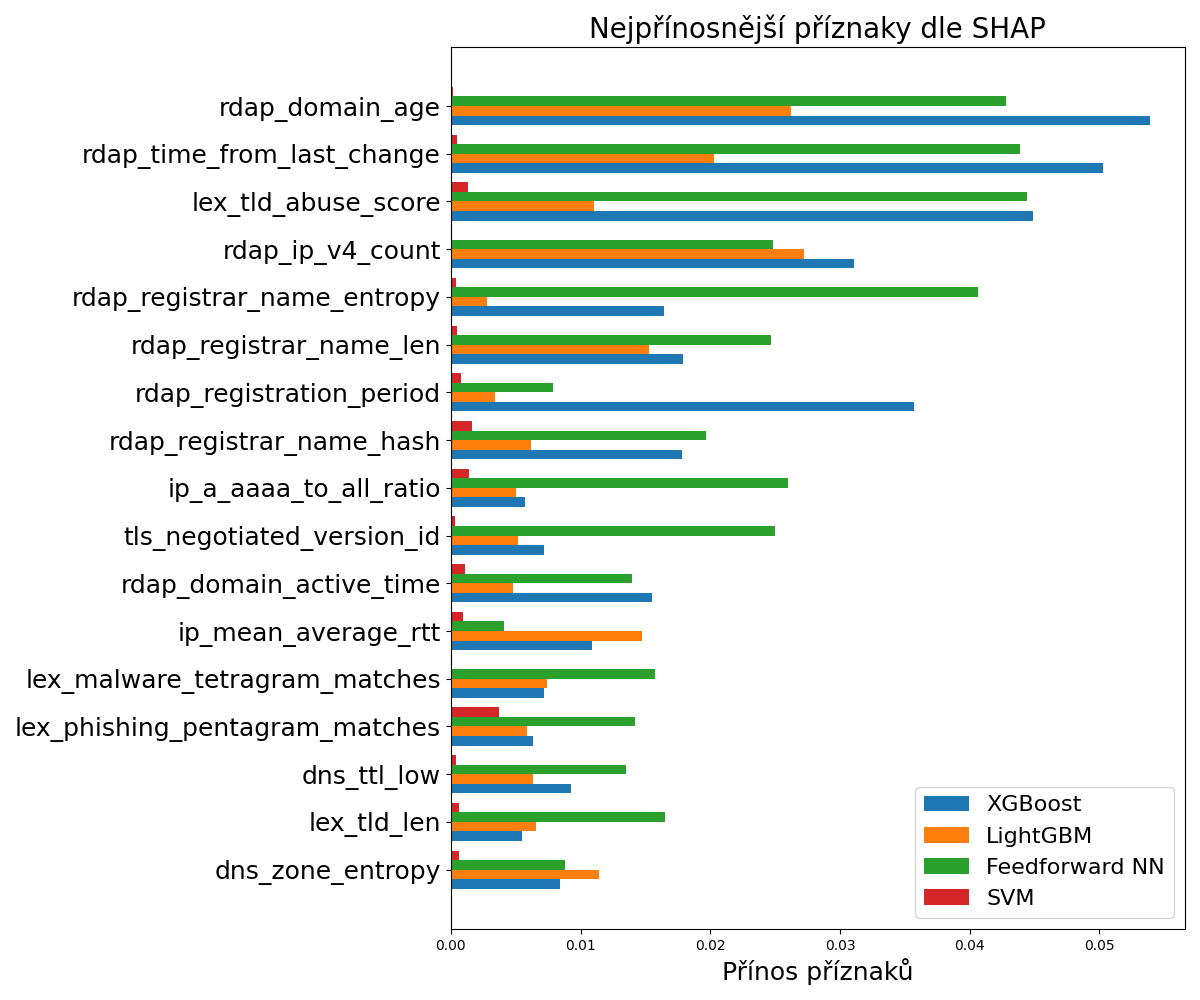
\includegraphics[width=0.95\textwidth]{obrazky-figures/top_10_shap.png}
    \caption{Nejpřínosnější příznaky napříč modely}
    \label{fig:top10shap}
\end{figure}

\subsection*{Závěry výsledků analýzy SHAP}

Z~analýzy metodou SHAP vyplývá několik klíčových poznatků:
\begin{itemize}
    \item Vysoká konzistence významných příznaků napříč modely potvrzuje jejich robustnost.
    \item RDAP a časové atributy dominují, což je v~souladu s~předpokladem, že škodlivé domény bývají často mladé, krátkodobě zaregistrované nebo podezřele upravované.
    \item Lexikální vlastnosti jako výskyt phishingových nebo malware n-gramů poskytují silnou diskriminaci i bez nutnosti síťových dotazů.
\end{itemize}

\section{Srovnání s~existujícími přístupy}
\label{sec:discussion-comparison}

Pro objektivní zhodnocení navrženého řešení byla provedena replikace vybraných studií (viz kapitola~\ref{sec:feature-survey}), jejichž přístupy byly implementovány a testovány na jednotné datové sadě. Všechny modely byly trénovány ve srovnatelných podmínkách a vyhodnoceny stejnou metodikou.

Tabulka~\ref{tab:method_comparison_final} shrnuje nejlepší dosažené hodnoty skóre F1 pro jednotlivé modely převzaté z~literatury, doplněné o~výsledky této práce. V~závěru tabulky jsou uvedeny dva řádky odpovídající výstupům vícestupňové pipeline s~rozhodovacím metamodulem – samostatně pro detekci phishingových a malware domén.

\begin{table}[H]
  \centering
  \begin{tabular}{@{}lcccccc@{}}
    \toprule
    \textbf{První autor} & \textbf{Rok} & \textbf{Typ} &
    \textbf{Nejlepší F1} & \textbf{\# f.} &
    \textbf{Kat.\ přízn.} & \textbf{Model}\\
    \midrule
    Torroledo   & 2018 & Malw   & 0.966 & 30  & TLS           & LightGBM\\
    Shi         & 2017 & Mix    & 0.915 & 9   & MIX           & LightGBM\\
    Magalhães   & 2020 & Mix    & 0.969 & 17  & MIX           & LightGBM\\
    Zhu         & 2019 & Mix    & 0.910 & 11  & MIX           & AdaBoost\\
    Kumar       & 2022 & Malw   & 0.932 & 15  & LEX           & AdaBoost\\
    Silveira    & 2021 & Mix    & 0.921 & 19  & DNS           & SVM\\
    Iwahana     & 2021 & Mix    & 0.968 & 25  & MIX           & LightGBM\\
    Gopinath    & 2020 & C\&C   & 0.937 & 17  & WHOIS+DNS     & LightGBM\\
    Hason       & 2020 & Mix    & 0.971 & 9   & MIX           & LightGBM\\
    Chatterjee  & 2019 & Phish  & 0.924 & 14  & MIX           & XGBoost\\
    Sadique     & 2020 & Phish  & 0.924 & 20  & MIX           & XGBoost\\
    \rowcolor{gray!10}
    \textbf{Tato práce} & 2025 & \textbf{Phish} & \textbf{0.985} & 176 & MULTI & Ensemble\\
    \rowcolor{gray!10}
    \textbf{Tato práce}  & 2025 & \textbf{Malw}  & \textbf{0.980} & 176 & MULTI & Ensemble\\
    \bottomrule
  \end{tabular}
  \caption{Srovnání s~replikovanými studiemi\newline%
    {\small Malw – malware, Phish – phishing, C\&C – command\&control, Mix – obecně škodlivé domény}}
  \label{tab:method_comparison_final}
\end{table}

Z~výsledků je patrné, že navržený přístup založený na skládání klasifikátorů (ensemble) nejen konkuruje nejlepším modelům z~literatury, ale v~obou sledovaných třídách je výrazně překonává. Výsledky potvrzují, že kombinovaný přístup dokáže přesněji rozlišit jemné znaky typické pro různé typy škodlivých domén a současně zachovat nízkou chybovost, což je klíčové pro praktické nasazení v~produkčních systémech. 

Mezi možné důvody tohoto zlepšení patří zejména použití rozsáhlejšího vektorového prostoru příznaků – v~rámci této práce bylo využito až 176 různých příznaků zahrnujících informace z~TLS, DNS, RDAP, GeoIP a lexikální analýzy, zatímco většina srovnávaných přístupů v~literatuře pracovala s~řádově desítkami příznaků. Vyšší granularita vstupních dat tak umožňuje modelům zachytit širší spektrum charakteristik domén.

Dalším přínosem je využití různorodých klasifikačních metod – konkrétně neuronových sítí, stromových algoritmů a podpůrných vektorových strojů – jejichž predikce jsou následně kombinovány v~rozhodovacím metamodelu. Tento kombinovaný přístup využívá silných stránek jednotlivých modelů a zmírňuje jejich individuální slabiny, což vede k~vyšší robustnosti celého systému. 

Oproti většině replikovaných prací navíc navržená pipeline poskytuje modulární architekturu, umožňující snadné rozšíření a přizpůsobení požadavkům konkrétního provozního prostředí. Díky tomu lze celý systém snadno aktualizovat o~nové příznaky, modely či detekční logiky bez nutnosti zásahu do základní infrastruktury.


\chapter{Diskuze}
\label{chapter:discussion}\label{chapter:10}


Tato kapitola shrnuje hlavní poznatky diplomové práce, hodnotí dosažené výsledky z~pohledu výkonnosti navržených klasifikátorů, diskutuje jejich praktické využití, upozorňuje na možná omezení navrženého řešení a reflektuje jeho etické dopady. Na závěr jsou diskutovány směry, jimiž by mohl výzkum dále pokračovat.

Navržená klasifikační pipeline byla experimentálně ověřena na dvou úrovních — na validační sadě, která vznikla oddělením testovací části datové sady. Dále proběhlo ověření na zcela nezávislé verifikační sadě, která byla získaná v~jiném časovém období. Podrobnější popis verifikační datové sady nalezneme v~sekci \ref{clftest}.

Na validační sadě dosáhl systém průměrné přesnosti \textbf{0{,}9875} a \textbf{skóre F1 0{,}9837}, čímž potvrdil vysokou stabilitu i přesnost při klasifikaci domén. Na verifikační sadě, která reprezentuje zcela nová a dříve neviděná data, pak systém dosáhl přesnosti \textbf{0{,}9536} a \textbf{skóre F1 0{,}9413}. Tyto výsledky potvrzují dobrou generalizační schopnost systému a jeho robustnost vůči datovému posunu.


\section{Zhodnocení klasifikátorů}
\label{sec:discussion-evaluation}

Výsledky experimentální části ukazují, že žádná jednotlivá klasifikační metoda neposkytuje univerzálně nejlepší výsledky ve všech scénářích. Nejlepší samostatně fungující model byl jednoznačně \textbf{XGBoost}, který dosahoval špičkových hodnot \textbf{skóre F1} zejména v~nižších stupních klasifikace, a zároveň se vyznačuje mimořádně nízkou výpočetní náročností, což z~něj činí atraktivního kandidáta pro nasazení v~reálném čase. Ve scénářích s~omezeným množstvím vstupních příznaků (Stage~1) byl XGBoost výrazně výkonnější než ostatní modely, a to jak z~hlediska přesnosti, tak rychlosti inferenčního běhu.

Vysokého skóre dosáhly i další modely. \textbf{Konvoluční neuronová síť} (CNN) dominovala ve třetím stupni (Stage~3), kde díky plnému vektoru 176 příznaků dokázala přesně zachytit komplexní vzory charakteristické pro maligní domény. Tento výsledek podporuje hypotézu o~vyšší účinnosti konvolučních neuronových sítí pro rozsáhlé vektory příznaků. Výrazně se osvědčila zejména v~klasifikaci phishingových domén, kde dosáhla \textbf{skóreF1 0{,}9654} a úplnost (recall) 0{,}9435, což naznačuje její vysokou schopnost rozpoznat jemné znaky typické pro tuto kategorii. Naopak v~případě malware domén její výkon výrazně poklesl – například recall zde činil pouze \textbf{0{,}6048} a skóre F1 \textbf{0{,}7451}, což může ukazovat na nedostatečné zachycení specifických vzorů této třídy, případně na větší variabilitu v~datech. 

SVM model vykazoval stabilní výkonnost napříč stupni klasifikace a ukázal se jako spolehlivá opora v~rozhodovacím metamodelu.

Při kombinaci výstupů těchto modelů prostřednictvím rozhodovacího metamodulu se podařilo dále zvýšit průměrné \textbf{skóre F1 až na 0{,}984} a snížit \textbf{míru falešně pozitivních klasifikací na 0{,}27\,\%}. Tímto byl překonán i nejlepší samostatný model, a to o~více než 1{,}8 procentního bodu v~AUC, což dokládá efektivitu hybridního přístupu.

Zajímavým zjištěním je, že různé klasifikační algoritmy vykazují zcela odlišné rozložení přínosu jednotlivých příznaků. Tento jev lze interpretovat jako důkaz toho, že jednotlivé modely se při rozhodování opírají o~odlišné aspekty vstupních dat a nacházejí různé vzory. To dále podporuje myšlenku využití kombinace více klasifikátorů, které se vzájemně doplňují a společně přispívají ke zvýšení robustnosti celého systému.

\textbf{HTML příznaky} sice v~rámci dílčích experimentů uvedených v~kapitole~\ref{chapter:7}, sekci~\ref{subsection:standalone_res}, vykazovaly u~vybraných podmnožin určitý potenciál, avšak při rozšířeném testování s~postupně akumulovanými skupinami příznaků se ukázalo, že jejich celkový přínos je zanedbatelný. Ačkoli se v~odborné literatuře objevují úspěšné aplikace detekce škodlivých domén právě na základě HTML charakteristik \cite{mahmood2021html}, v~této konkrétní implementaci nebyly tyto příznaky schopny významně zlepšit klasifikační výkon. Z~toho důvodu nebyly zahrnuty do finálního vektorového prostoru a následných klasifikací.


Při analýze výstupů metamodelu bylo rovněž identifikováno několik anomálních případů, kdy byl doménový záznam klasifikován jako maligní navzdory přítomnosti atributů typických pro legitimní provoz (např. validní certifikát vystavený známou autoritou). Podrobnější inspekce těchto případů ukázala, že šlo často o~domény s~krátkou životností a podezřelou geolokací IP adresy, což naznačuje, že metamodel dokáže zachytit i jemné kontextové signály, které by jednotlivé modely mohly přehlédnout. Tato schopnost spojit částečné informace z~více zdrojů je klíčovým přínosem celé pipeline.



\section{Praktické dopady práce}
\label{sec:discussion-impact}

Výsledky této práce mají přímé praktické uplatnění v~oblasti síťové bezpečnosti a automatizované detekce kybernetických hrozeb. Navržený klasifikační systém je navržen s~důrazem na škálovatelnost, odolnost a flexibilitu, a je plně připraven k~nasazení v~prostředí nástroje \emph{DomainRadar}, jehož cílem je v~reálném čase vyhodnocovat rizikovost domén.

Díky \textbf{vícestupňové architektuře} umožňuje pipeline adaptivní rozhodování podle dostupnosti dat a požadavků na výpočetní náročnost. První stupeň (Stage~1) využívá pouze rychle dostupné lexikální a statistické příznaky a dokáže provést hrubou klasifikaci v~řádu milisekund. Tato schopnost je klíčová v~prostředích s~omezenou latencí, například při inspekci síťového provozu na perimetru. V~případech, kdy je doména vyhodnocena jako podezřelá nebo se nachází v~hraniční oblasti rozhodnutí, systém umožňuje dynamicky stáhnout doplňující informace (např. záznamy RDAP, údaje o~TLS certifikátech) a následně doménu překlasifikovat ve vyšším stupni (Stage~2 nebo Stage~3). Pokud ani poté není jistota dostatečná, je výstup přesměrován k~\textbf{manuální revizi}, což nabízí větší možnost kontroly nad systémem a snižuje falešně pozitivní výsledky. 

Významným přínosem navrženého řešení je také \textbf{snížení počtu falešně pozitivních detekcí}, které v~systémech typu SIEM často vedou k~zahlcení operátorů a ztrátě důvěry ve varovné signály. Integrace \textit{False Positive Detectoru} v~rámci pipeline umožňuje efektivní filtrování těchto případů a přispívá ke zlepšení celkové \textbf{věrohodnosti klasifikace}. 

Systém tak umožňuje lepší integraci do stávajících detekčních systémů, kde může sloužit jako samostatný modul nebo jako doplněk k~existujícím nástrojům.

\section{Omezení práce}
\label{sec:discussion-limitations}

Ačkoli systém dosáhl velmi dobrých výsledků na validační i verifikační sadě, je nutné objektivně poukázat na jeho omezení, která mohou ovlivnit jeho výkonnost a možnosti reálného provozu.

\begin{itemize}
    \item \textbf{Nevyváženost tříd}. Základní charakteristikou použité datové sady je nevyváženost mezi benigními a maligními doménami. Ačkoliv byla během trénování modelů zohledněna prostřednictvím vah ztrátové funkce a selektivního resamplingu, nelze zcela vyloučit vznik mírného biasu vůči většinové třídě. To může vést k~mírnému snížení citlivosti u~menšinové třídy, zejména v~okrajových případech.

    \item \textbf{Závislost na kvalitě dat}. Přesnost klasifikace je významně ovlivněna kvalitou trénovací a testovací sady. Použitá anotovaná data pocházejí ze zdrojů třetích stran, jako jsou \emph{PhishTank}, \emph{VirusTotal} nebo \emph{URLHaus}. I~když jde o~renomované databáze, jejich anotace nemusí být vždy aktuální nebo zcela bezchybné. Model tak může být částečně ovlivněn případnými chybně zařazenými vzorky.

    \item \textbf{Stárnutí modelů}. Charakteristiky maligních domén nejsou neměnné. V~čase se vyvíjejí taktiky útočníků, struktura domén i jejich metadata. Bez průběžné aktualizace modelu, případně bez zavedení mechanismu pro \emph{kontinuální přeučování}, může docházet k~degradaci klasifikační výkonnosti. Reálné nasazení modelu by proto mělo zahrnovat periodické monitorování jeho přesnosti a zavedení procesů pro jeho aktualizaci na základě nově získaných dat.
\end{itemize}



\section{Etické aspekty}
\label{sec:discussion-ethics}

Při návrhu a realizaci této práce byl kladen důraz na respektování etických zásad a ochranu soukromí. Veškerá zpracovávaná data jsou veřejně dostupná a týkají se výhradně doménových jmen a jejich technických parametrů. Práce neobsahuje žádné osobní ani citlivé údaje o~konkrétních jednotlivcích, a veškerá data byla anonymizována již ve fázi sběru.

Nicméně v~případě nasazení klasifikačního systému do reálného provozu, například v~rámci filtrování síťového provozu, je nezbytně nutné zohlednit etické dopady automatického rozhodování. Zvláště v~kontextu \textbf{blokace domén} na základě výstupu modelu může dojít k~následujícím rizikům:

\begin{enumerate}[label=(\alph*)]
    \item \textbf{Zablokování legitimních webů} – i přes vysokou přesnost systému a implementaci detektoru falešně pozitivních případů nelze vyloučit situaci, kdy bude chybně označena legitimní doména, což může negativně ovlivnit reputaci subjektu, způsobit výpadek služeb nebo poškodit uživatelskou důvěru.
    
    \item \textbf{Nedostatek vysvětlitelnosti} – rozhodnutí založená na strojovém učení nemusí být snadno interpretovatelná koncovými uživateli či správci. Tato „černá skříňka“ může být problematická zejména v~případech, kdy je vyžadováno zdůvodnění rozhodnutí.
\end{enumerate}

Z~těchto důvodů je nutné, aby byl systém v~praxi doplněn o~proces \textbf{lidské revize} pro rozhodnutí v~hraničních případech, nebo v~případech s~vysokým dopadem.

Jako doplněk k~systému by měl být navržen \textbf{mechanismus odvolání} umožňující přezkoumání v~případě sporné klasifikace. Automatizované nástroje by měly sloužit jako podpora rozhodování, nikoliv jako jeho jediný arbitrážní mechanismus.


\section{Budoucí směřování práce}
\label{sec:discussion-future}

Možnosti dalšího rozvoje navrženého řešení jsou rozsáhlé, a to jak na úrovni výzkumu, tak v~oblasti praktické aplikace. Některé z~navržených směrů budoucí práce zahrnují následující:

\begin{itemize}
    \item \textbf{Integrace do systému DomainRadar}. Hlavním cílem následujících fází vývoje je kompletní integrace navržené pipeline do platformy DomainRadar, včetně napojení na systém sběru živých dat a uživatelského rozhraní. To umožní validaci výsledků na datech z~produkčního provozu a vyhodnocení přínosu v~reálných podmínkách.

    \item \textbf{Měření výkonnosti v~provozu}. Po nasazení bude možné kvantifikovat vliv systému na snížení množství falešně pozitivních detekcí, zrychlení reakční doby a zvýšení efektivity práce bezpečnostních analytiků.

    \item \textbf{Výzkum časové degradace modelů}. Plánuje se sledování výkonnosti klasifikátorů v~čase, analýza jejich postupné degradace a návrh metrik, které umožní včasné rozpoznání potřeby přetrénování. Tento výzkum bude klíčový pro dlouhodobé nasazení systému v~dynamickém prostředí.

    \item \textbf{Zavedení kontinuálního učení}. Na základě poznatků o~časovém driftu se předpokládá zavedení mechanismu pro \textbf{průběžné aktualizace modelů}, a to buď pomocí batch retrainingu, nebo prostřednictvím online learning technik. Tyto přístupy umožní rychle reagovat na nové typy hrozeb a zamezit degradaci přesnosti.

    \item \textbf{Rozšíření datové sady}. Budoucí práce by měla usilovat o~další rozšíření množství i rozmanitosti vstupních dat. Zvláštní pozornost bude věnována akvizici domén z~méně pokrytých jazykových a geografických oblastí, čímž se zvýší generalizační schopnost systému.
\end{itemize}



\chapter{Závěr}
\label{chapter:conclusion}

Tato diplomová práce se zaměřila na porovnání klasifikačních metod pro detekci maligních domén a na návrh klasifikačního systému na bázi spojování těchto modelů. V~průběhu práce byly analyzovány a implementovány modely jako Support Vector Machine (SVM), neuronové sítě různých architektur a stromové algoritmy, přičemž hlavní důraz byl kladen na optimalizaci parametrů a zpracování nevyvážených dat.

Výsledky experimentální části ukázaly, že žádný z~jednotlivých modelů neposkytuje univerzálně nejlepší výkonnost napříč všemi klasifikačními stupni. V~rámci vícestupňové architektury se pro každý stupeň optimalizovalo více modelů, přičemž nejlepší výsledky v~jednotlivých fázích byly následující.

V~prvním stupni, který využívá pouze lexikální příznaky, dosáhla nejlepších výsledků dopředná neuronová síť se skóre F1 ve výši 0{,}8942 pro phishing a 0{,}8841 pro malware. Ve druhém stupni, který rozšiřuje vstupní vektor o~informace z~externích zdrojů (např. WHOIS, DNS), vykázal nejvyšší výkonnost model LightGBM — skóre F1 činilo 0{,}9638 pro phishing a 0{,}9639 pro malware. Modely v~této fázi již poskytují vysoce spolehlivé rozhodování a vykazují nízkou chybovost. 

Ve třetím stupni, kde jsou k~dispozici všechny příznaky včetně dat z~RDAP, dosáhl nejlepší výkonnosti model XGBoost. Pro phishing činilo skóre F1 0{,}9860 a pro malware 0{,}9744. Průměrné skóre F1 tohoto modelu tak dosahuje 0{,}9802 při míře falešně pozitivních detekcí 0{,}19\,\%.

Tento výsledek potvrzuje vhodnost stromových algoritmů pro komplexní datové reprezentace a zároveň ukazuje na výrazné zvýšení detekční přesnosti ve finálním rozhodovacím stupni.

Po sloučení výstupů těchto modelů do vícestupňové pipeline řízené rozhodovací neuronovou sítí došlo ke zlepšení celkové výkonnosti systému. Bylo dosaženo průměrného skóre F1 0{,}9837, přičemž pro phishing činilo 0{,}9875 a pro malware 0{,}980. Míra falešně pozitivních detekcí přitom klesla z~0{,}27\,\% na 0{,}19\,\%. Zvýšení skóre F1 a snížení míry falešně pozitivních výsledků oproti nejlepšímu samostatnému klasifikátoru potvrzují, že hybridní přístup přináší vyšší přesnost, robustnost a schopnost generalizace.

Srovnání s~vybranými pracemi z~literatury dále potvrdilo, že navržený přístup dosahuje nejvyšších hodnot skóre F1 ve všech sledovaných třídách. Zatímco nejlepší replikované přístupy dosahovaly maximálních hodnot skóre F1 kolem 0{,}97, navržená pipeline tyto výsledky překonává. Dobré výsledky lze přičíst použití rozsáhlejší množiny 176 příznaků. Tyto příznaky kombinují informace z~TLS, DNS, RDAP, GeoIP a lexikální analýzy, čímž poskytují detailnější popis doménových charakteristik než přístupy pracující s~nižším počtem vstupních prvků. Kombinovaná strategie umožňuje využít silných stránek různých klasifikátorů a zároveň zmírňuje jejich slabiny. To se v~praxi projevuje lepší generalizací a nižší mírou chybovosti než u~dříve publikovaných řešení.

Součástí práce byl také návrh a implementace metody Gradient Grid Search pro efektivní ladění hyperparametrů, inspirované principy gradientního sestupu. Tato metoda přispěla ke zrychlení experimentální fáze při zachování kvality výsledků a překonává tradiční přístup grid-search zejména ve vysokodimenzionálních prostorech.

Z~hlediska praktického nasazení se navržený systém jeví jako perspektivní řešení jak pro akademické účely, tak pro reálné bezpečnostní infrastruktury. Vícestupňová architektura umožňuje adaptivní rozhodování na základě dostupnosti dat a výpočetních zdrojů, čímž zajišťuje efektivní klasifikaci i v~prostředích s~omezenou latencí a zdroji. Systém je zároveň navržen tak, aby byl snadno rozšiřitelný o~další příznaky a modely a umožňoval integraci do větších detekčních platforem, jako je například nástroj DomainRadar.

Další směřování práce by mělo zahrnovat rozšíření datové sady o~dynamické síťové příznaky a využití pokročilejších architektur hlubokého učení, zejména transformerových modelů. Rovněž je vhodné zkoumat možnosti aktivního a online učení, které umožní adaptivní aktualizaci modelů v~reálném čase na základě nových dat. Pozornost by měla být věnována také sledování časové degradace modelů a návrhu mechanismů pro jejich pravidelné dotrénování.

V~rámci práce vznikla rovněž sada vědeckých publikací, které dále rozvíjejí její dílčí výstupy. Jejich přehled je uveden v~příloze~\ref{appendix:publications}.

Závěrem lze konstatovat, že diplomová práce splnila vytyčené cíle, přinesla nové poznatky v~oblasti detekce škodlivých domén a představuje pevný základ pro další výzkum i praktické využití v~oblasti kybernetické bezpečnosti.



% Koniec filma

  \fi
  
  % Kompilace po částech (viz výše, nutno odkomentovat)
  % Compilation piecewise (see above, it is necessary to uncomment it)
  %\subfile{projekt-01-uvod-introduction}
  % ...
  %\subfile{chapters/projekt-05-conclusion}


  % Pouzita literatura / Bibliography
  % ----------------------------------------------
\ifslovak
  \makeatletter
  \def\@openbib@code{\addcontentsline{toc}{chapter}{Literatúra}}
  \makeatother
  \bibliographystyle{bib-styles/Pysny/skplain}
\else
  \ifczech
    \makeatletter
    \def\@openbib@code{\addcontentsline{toc}{chapter}{Literatura}}
    \makeatother
    \bibliographystyle{bib-styles/Pysny/czplain}
  \else 
    \makeatletter
    \def\@openbib@code{\addcontentsline{toc}{chapter}{Bibliography}}
    \makeatother
    \bibliographystyle{bib-styles/Pysny/enplain}
  %  \bibliographystyle{alpha}
  \fi
\fi
  \begin{flushleft}
  \bibliography{projekt-20-literatura-bibliography}
  \end{flushleft}

  % vynechani stranky v oboustrannem rezimu
  % Skip the page in the two-sided mode
  \iftwoside
    \cleardoublepage
  \fi

  % Prilohy / Appendices
  % ---------------------------------------------
  \appendix
\ifczech
  \renewcommand{\appendixpagename}{Přílohy}
  \renewcommand{\appendixtocname}{Přílohy}
  \renewcommand{\appendixname}{Příloha}
\fi
\ifslovak
  \renewcommand{\appendixpagename}{Prílohy}
  \renewcommand{\appendixtocname}{Prílohy}
  \renewcommand{\appendixname}{Príloha}
\fi
%  \appendixpage

% vynechani stranky v oboustrannem rezimu
% Skip the page in the two-sided mode
%\iftwoside
%  \cleardoublepage
%\fi
  
\ifslovak
%  \section*{Zoznam príloh}
%  \addcontentsline{toc}{section}{Zoznam príloh}
\else
  \ifczech
%    \section*{Seznam příloh}
%    \addcontentsline{toc}{section}{Seznam příloh}
  \else
%    \section*{List of Appendices}
%    \addcontentsline{toc}{section}{List of Appendices}
  \fi
\fi
  \startcontents[chapters]
  \setlength{\parskip}{0pt} 
  % seznam příloh / list of appendices
  % \printcontents[chapters]{l}{0}{\setcounter{tocdepth}{2}}
  
  \ifODSAZ
    \setlength{\parskip}{0.5\bigskipamount}
  \else
    \setlength{\parskip}{0pt}
  \fi
  
  % vynechani stranky v oboustrannem rezimu
  \iftwoside
    \cleardoublepage
  \fi
  
  % Přílohy / Appendices
  \ifenglish
    \input{projekt-30-prilohy-appendices-en}
  \else
    \chapter{Obsah přiloženého paměťového média}
V přiloženém digitálním úložišti se nalézá:
\begin{itemize}
    \item tento dokument ve formátu PDF,
    \item zdrojové soubory tohoto dokumentu,
    \item zdrojové kódy vyvinutého klasifikačního systému,
    \item klasifikátory které vznikly v~rámci této práce,
    \item trénovací, validační a verifikační datové sady,
    \item návod k~použití přiloženého klasifikačního systému.
\end{itemize}





\chapter{Manuál}

Veškerý zdrojový kód, trénovací skripty, výsledky experimentů i příklady použití klasifikační pipeline jsou volně dostupné v~repozitáři na platformě Github:

\begin{center}
\url{https://github.com/poli-cz/Domain-Ensemble-pipeline}
\end{center}

\noindent Tento repozitář slouží jako praktický doplněk k~této diplomové práci a umožňuje plnou replikaci a rozšíření prezentovaného řešení.

\section*{Přiložený software}

Repozitář obsahuje kompletní implementaci vícestupňové klasifikační pipeline určené pro detekci maligních domén. Kromě samotného systému zahrnuje také sadu předtrénovaných modelů, podpůrné utility pro načítání dat, vizualizaci výstupů a moduly pro výpočet interpretací pomocí SHAP analýzy.

\subsection*{Trénování klasifikátorů}

Trénovací skripty jsou připraveny ve formě Jupyter notebooků a jsou umístěny ve složce:

\begin{verbatim}
src/training/
\end{verbatim}

Pro každý klasifikátor je připraven samostatný notebook:

\begin{itemize}
\item \texttt{feedforward\_train.ipynb} – trénink plně propojené neuronové sítě (FFNN)
\item \texttt{cnn\_train.ipynb} – trénink konvoluční neuronové sítě (CNN)
\item \texttt{svm\_train.ipynb} – trénink klasifikátoru svm
\item \texttt{xgb\_lgbm\_train.ipynb} – trénink stromových modelů (XGBoost a LightGBM)
\item \texttt{meta\_model\_train.ipynb} – trénink rozhodovacího meta-modelu a modulu pro detekci falešně pozitivních vzorků (FPD)
\end{itemize}

\noindent Trénink probíhá na vstupních datasetech ve formátu .parquet, které je nutné stáhnout samostatně (například z~repozitáře \texttt{domainradar-clf}) a umístit do složky:

\begin{verbatim}
src/parkets/
\end{verbatim}

\subsection*{Běh klasifikačního systému}

Pro spuštění klasifikační pipeline na nových doménách slouží notebook:

\begin{verbatim}
src/ensemble_pipeline_example.ipynb
\end{verbatim}

V~tomto notebooku je demonstrováno:

\begin{itemize}
\item inicializace pipeline včetně načtení předtrénovaných modelů
\item klasifikace vstupních vzorků domén
\item volitelná interpretace výstupu pomocí SHAP hodnot
\end{itemize}

Pipeline automaticky detekuje dostupnost jednotlivých příznakových kategorií (lexikální, DNS, RDAP, TLS apod.) a adaptivně zvolí odpovídající klasifikační model.

Konkrétní verze použitých modelů lze upravit ve skriptu:

\begin{verbatim}
src/pipeline.py
\end{verbatim}

\section*{Adresáře}
\label{sec:adresare}

Tato sekce přílohy stručně popisuje strukturu repozitáře, který obsahuje implementaci klasifikační pipeline pro detekci škodlivých domén. Systém tvoří samostatný, plně funkční modul pro trénink, inferenci a vyhodnocování modelů. Repozitář je rozdělen do adresářů podle funkce jednotlivých komponent:

\begin{itemize}
    \item \textbf{/src} – Hlavní adresář s~implementací klasifikační pipeline. Obsahuje datové transformace, načítání modelů, tréninkové notebooky, SHAP analýzu, i demonstrační příklad použití.
    
    \item \textbf{/src/core} – Základní komponenty pipeline: načítání a segmentace dat, modely metaklasifikace, detekce falešně pozitivních vzorků, a pomocné utility.
    
    \item \textbf{/src/models} – Vytrénované modely všech architektur (Keras, LightGBM, SVM, XGBoost) a jejich potřebné scalery. Obsahuje i samostatné složky pro metamodel a FPD modul.
    
    \item \textbf{/src/scalers} – Předtrénované modely pro normalizace a škálování uložené pomocí knihovny \texttt{joblib}, potřebné při inferenci dat.
    
    \item \textbf{/src/data} – Serializované validační a verifikační datasety (ve formátu \texttt{.pkl}) pro jednotlivé fáze klasifikace.
    
    \item \textbf{/src/parkets} – Vstupní datasety ve formátu \texttt{parquet}. Obsahuje anonymizovaná i neanonymizovaná data, HTML varianty, a testovací podmnožiny.
    
    \item \textbf{/src/results} – Výstupní grafy a výsledky vyhodnocení, např. konfuzní matice modelů.
    
    \item \textbf{/src/tmp} – Dočasné a experimentální výstupy vzniklé během ladění pipeline, např. serializované výsledky, podmnožiny datasetů, nebo mezivýstupy modelů.
    
    \item \textbf{/src/training} – Trénovací Jupyter notebooky pro jednotlivé modely: FFNN, CNN, SVM, LightGBM/XGBoost, attention modely a metamodel.
    
    \item \textbf{/src/tex\_sources} – Pomocné \LaTeX{} soubory a tabulky s~metrikami, použité při psaní práce.
    
    \item \textbf{/src/ensemble\_pipeline\_example.ipynb} – Příkladový notebook demonstrující kompletní klasifikaci vstupních domén pomocí finální pipeline.
    
    \item \textbf{/docs} – Dokumentace a podpůrné materiály k~diplomové práci, zejména vizualizace, diagramy a SHAP grafy.
    
    \item \textbf{/docs/figures} – Všechny výstupní obrázky, včetně agregovaných výsledků, SHAP analýz, architektur a porovnání.
    
    \item \textbf{/docs/figures/confusion\_matrices} – Konfuzní matice všech modelů ve všech fázích tréninku a verifikace.
    
    \item \textbf{/docs/tex\_sources} – Soubory použitých LaTeX tabulek, sloupcových dat a automaticky generovaných výsledků metrik.
    
    \item \textbf{/experiments} – Experimenty s~mřížkami příznaků, porovnání modelů, SHAP analýzou a ladění pipeline.
    
    \item \textbf{/experiments/grids} – CSV soubory obsahující výsledky mřížkových vyhodnocení příznakových subsetů pro phishing i malware.
    
    \item \textbf{/experiments/shap} – SHAP analýzy, skripty a záložní výstupy přínosů jednotlivých příznaků pro vybrané modely.
    
    \item \textbf{/tests} – Jednotkové testy pro ověření základní funkčnosti vybraných komponent pipeline.
    
    \item \textbf{README.md} – Úvodní dokumentace repozitáře (v~anglickém jazyce), s~návodem na spuštění, trénink a inferenci.
    
    \item \textbf{poetry.lock, pyproject.toml} – Konfigurační soubory pro správu Python prostředí pomocí nástroje \texttt{Poetry}.
\end{itemize}
\chapter{Publikační činnost}
\label{appendix:publications}

S~touto diplomovou prací úzce souvisí několik vědeckých publikací, na jejichž jsem spoluautorem. Tyto publikace vznikly v~průběhu řešení práce a pokrývají různé aspekty detekce maligních domén.

\begin{itemize}
    \item \textbf{Unmasking the Phishermen: Phishing Domain Detection with Machine Learning and Multi-Source Intelligence}  
    (publikováno na konferenci \textit{IEEE/IFIP Network Operations and Management Symposium (NOMS 2024)})  
    Článek se zabývá detekcí phishingových domén pomocí kombinace vícerozdrojových dat (DNS, RDAP, TLS, IP) a využívá ensemble modely pro zvýšení přesnosti klasifikace. Zvláštní důraz je kladen na reálnou aplikovatelnost modelů a nízkou míru falešně pozitivních detekcí \cite{noms}.

    \item \textbf{Spotting the Hook: Leveraging Domain Data for Advanced Phishing Detection}  
    (publikováno na konferenci \textit{IEEE CNSM 2024})  
    Publikace představuje 143položkový příznakový vektor pro phishingovou klasifikaci a hodnotí jeho efektivitu napříč sedmi strojově učenými modely. Výsledky ukazují velmi vysokou přesnost (0{,}983) a nízkou chybovost díky využití multi-modalních vstupních dat \cite{CNSM}.

    \item \textbf{A~Multi-Dimensional DNS Domain Intelligence Dataset for Cybersecurity Research}  
    (v~recenzním řízení, žurnál \textit{Data in Brief})  
    Tento článek popisuje rozsáhlou datovou sadu více než 1 milionu anotovaných domén (benigních, phishingových a malware), včetně metodologie sběru, transformace a kategorizace dat ze čtyř hlavních zdrojů: DNS, RDAP, TLS a GeoIP.

    \item \textbf{Digital Wolves in Sheep’s Clothing: Detecting Malicious Domains using a Multi-Stage Classifier Pipeline}  
    (v~přípravě, žurnál \textit{IEEE Access})  
    Článek se věnuje návrhu a experimentálnímu vyhodnocení vícestupňové klasifikační pipeline s~paralelními modely, rozhodovacím metaklasifikátorem a modulem pro detekci falešných pozitiv. Přímým základem článku je implementace uvedená v~této práci.

    \item \textbf{DomainRadar: A~Data-Driven Approach to Malicious Domain Identification}  
    (v~přípravě, žurnál \textit{IEEE Transactions on Information Forensics and Security (TIFS)})  
    Tento článek popisuje vývoj a architekturu systému \textit{DomainRadar}, který integruje výsledky této práce do automatizovaného nástroje pro detekci maligních domén v~síťovém provozu. Zaměřuje se na praktické nasazení v~prostředí bezpečnostních analytiků a SOC týmů.
\end{itemize}

\chapter{Přehled použitých příznaků}

\label{app:feature_vector}

V~této příloze je uvedena kompletní tabulka použitých příznaků (feature vektor), které byly analyzovány a využívány v~klasifikátorech v~rámci této práce. Celkem se jedná o~243 příznaků. 

\begin{longtable}{@{}ll@{}}
\caption{Overview of used features}\\
\toprule
\textbf{Feature name} & \textbf{Description} \\
\midrule
\endfirsthead

\toprule
\textbf{Feature name} & \textbf{Description} \\
\midrule
\endhead

\midrule
\multicolumn{2}{r}{\textit{Continued on next page}} \\
\midrule
\endfoot

\bottomrule
\endlastfoot

\multicolumn{2}{l}{\emph{Lexical features (lex\_)}} \\
lex\_name\_len & Length of the domain name \\
lex\_has\_digit & True if domain name contains a digit \\
lex\_phishing\_keyword\_count & Number of phishing keywords found \\
lex\_benign\_keyword\_count & Number of benign keywords found \\
lex\_consecutive\_chars & Longest consecutive character sequence \\
lex\_tld\_len & Length of the TLD \\
lex\_tld\_abuse\_score & Abuse score of the TLD \\
lex\_tld\_hash & Hash of the TLD \\
lex\_sld\_len & Length of the SLD \\
lex\_sld\_norm\_entropy & Normalised entropy of the SLD \\
lex\_sld\_digit\_count & Number of digits in the SLD \\
lex\_sld\_digit\_ratio & Ratio of digits in the SLD \\
lex\_sld\_phishing\_keyword\_count & Number of phishing keywords in SLD \\
lex\_sld\_vowel\_count & Number of vowels in SLD \\
lex\_sld\_vowel\_ratio & Ratio of vowels in SLD \\
lex\_sld\_consonant\_count & Number of consonants in SLD \\
lex\_sld\_consonant\_ratio & Ratio of consonants in SLD \\
lex\_sld\_non\_alphanum\_count & Number of non-alphanumeric chars in SLD \\
lex\_sld\_non\_alphanum\_ratio & Ratio of non-alphanumeric chars in SLD \\
lex\_sld\_hex\_count & Number of hex characters in SLD \\
lex\_sld\_hex\_ratio & Ratio of hex characters in SLD \\
lex\_sub\_count & Number of subdomains \\
lex\_stld\_unique\_char\_count & Unique characters in TLD+SLD \\
lex\_begins\_with\_digit & True if domain begins with digit \\
lex\_www\_flag & True if domain starts with 'www' \\
lex\_sub\_max\_consonant\_len & Longest consonant sequence in subdomain \\
lex\_sub\_norm\_entropy & Normalised entropy of subdomains \\
lex\_sub\_digit\_count & Number of digits in subdomains \\
lex\_sub\_digit\_ratio & Ratio of digits in subdomains \\
lex\_sub\_vowel\_count & Number of vowels in subdomains \\
lex\_sub\_vowel\_ratio & Ratio of vowels in subdomains \\
lex\_sub\_consonant\_count & Number of consonants in subdomains \\
lex\_sub\_consonant\_ratio & Ratio of consonants in subdomains \\
lex\_sub\_non\_alphanum\_count & Non-alphanumeric count in subdomains \\
lex\_sub\_non\_alphanum\_ratio & Ratio of non-alphanumerics in subdomains \\
lex\_sub\_hex\_count & Hex characters in subdomains \\
lex\_sub\_hex\_ratio & Ratio of hex in subdomains \\
lex\_phishing\_bigram\_matches & Phishing bigram matches \\
lex\_phishing\_trigram\_matches & Phishing trigram matches \\
lex\_phishing\_tetragram\_matches & Phishing tetragram matches \\
lex\_phishing\_pentagram\_matches & Phishing pentagram matches \\
lex\_malware\_bigram\_matches & Malware bigram matches \\
lex\_malware\_trigram\_matches & Malware trigram matches \\
lex\_malware\_tetragram\_matches & Malware tetragram matches \\
lex\_dga\_bigram\_matches & DGA bigram matches \\
lex\_dga\_trigram\_matches & DGA trigram matches \\
lex\_dga\_tetragram\_matches & DGA tetragram matches \\
lex\_avg\_part\_len & Average part length \\
lex\_stdev\_part\_lens & Standard deviation of part lengths \\
lex\_longest\_part\_len & Longest domain part length \\
lex\_short\_part\_count & Count of short domain parts \\
lex\_medium\_part\_count & Count of medium domain parts \\
lex\_long\_part\_count & Count of long domain parts \\
lex\_superlong\_part\_count & Count of superlong domain parts \\
lex\_shortest\_sub\_len & Shortest subdomain length \\
lex\_ipv4\_in\_domain & True if IPv4 in domain name \\
lex\_has\_trusted\_suffix & True if trusted suffix used \\
lex\_has\_wellknown\_suffix & True if well-known suffix used \\
lex\_has\_cdn\_suffix & True if CDN suffix used \\
lex\_has\_vps\_suffix & True if VPS suffix used \\
lex\_has\_img\_suffix & True if image suffix used \\
lex\_suffix\_score & Computed suffix score \\

\midrule
\multicolumn{2}{l}{\emph{DNS-based features (dns\_)}} \\
dns\_has\_dnskey & DNSKEY record present \\
dns\_A\_count & Number of A records \\
dns\_AAAA\_count & Number of AAAA records \\
dns\_MX\_count & Number of MX records \\
dns\_NS\_count & Number of NS records \\
dns\_TXT\_count & Number of TXT records \\
dns\_SOA\_count & Number of SOA records \\
dns\_CNAME\_count & Number of CNAME records \\
dns\_zone\_level & Zone domain level \\
dns\_zone\_digit\_count & Digits in zone domain \\
dns\_zone\_len & Zone domain length \\
dns\_zone\_entropy & Zone domain entropy \\
dns\_resolved\_record\_types & Number of RR types resolved \\
dns\_dnssec\_score & DNSSEC score (always zero) \\
dns\_ttl\_avg & Average TTL \\
dns\_ttl\_stdev & TTL standard deviation \\
dns\_ttl\_low & Count of TTL in [0,100] \\
dns\_ttl\_mid & Count of TTL in [101,500] \\
dns\_ttl\_distinct\_count & Distinct TTL values \\
dns\_soa\_primary\_ns\_level & Primary NS domain level \\
dns\_soa\_primary\_ns\_digit\_count & Digits in primary NS \\
dns\_soa\_primary\_ns\_len & Length of primary NS domain \\
dns\_soa\_primary\_ns\_entropy & Entropy of primary NS domain \\
dns\_soa\_email\_level & Admin email domain level \\
dns\_soa\_email\_digit\_count & Digits in admin email domain \\
dns\_soa\_email\_len & Length of admin email domain \\
dns\_soa\_email\_entropy & Entropy of admin email domain \\
dns\_soa\_refresh & SOA refresh value \\
dns\_soa\_retry & SOA retry value \\
dns\_soa\_expire & SOA expire value \\
dns\_soa\_min\_ttl & SOA minimum TTL \\
dns\_domain\_name\_in\_mx & MX is a subdomain of domain \\
dns\_mx\_avg\_len & Average length of MX names \\
dns\_mx\_avg\_entropy & Average entropy of MX names \\
dns\_txt\_avg\_len & Average TXT record length \\
dns\_txt\_avg\_entropy & Average entropy of TXT records \\
dns\_txt\_external\_verification\_score & Known verification strings in TXT \\
dns\_txt\_spf\_exists & SPF found in TXT records \\
dns\_txt\_dkim\_exists & DKIM found in TXT records \\
dns\_txt\_dmarc\_exists & DMARC found in TXT records \\

% Here the table would continue further: ip_, tls_, geo_, rdap_, html_
\midrule
\multicolumn{2}{l}{\emph{IP-based features (ip\_)}} \\
ip\_count & Number of IP addresses \\
ip\_mean\_average\_rtt & Average round-trip time (ICMP) \\
ip\_v4\_ratio & IPv4 to all IPs ratio \\
ip\_a\_aaaa\_to\_all\_ratio & A/AAAA to all IPs ratio \\
ip\_entropy & Entropy of IP prefixes (/16 and /64) \\
ip\_as\_address\_entropy & Entropy of AS address prefixes \\
ip\_asn\_entropy & Entropy of ASN numbers \\
ip\_distinct\_as\_count & Number of distinct ASNs \\

\midrule
\multicolumn{2}{l}{\emph{TLS-based features (tls\_)}} \\
tls\_has\_tls & True if TLS connection established \\
tls\_chain\_len & Certificate chain length \\
tls\_is\_self\_signed & True if certificate is self-signed \\
tls\_root\_authority\_hash & Hash of root authority name \\
tls\_leaf\_authority\_hash & Hash of leaf authority name \\
tls\_negotiated\_version\_id & Negotiated TLS version ID \\
tls\_negotiated\_cipher\_id & Negotiated TLS cipher ID \\
tls\_root\_cert\_validity\_len & Root certificate validity period \\
tls\_leaf\_cert\_validity\_len & Leaf certificate validity period \\
tls\_broken\_chain & Broken certificate chain present \\
tls\_expired\_chain & Expired certificate present \\
tls\_total\_extension\_count & Total number of certificate extensions \\
tls\_critical\_extensions & Number of critical extensions \\
tls\_with\_policies\_crt\_count & Number of certificates with policies \\
tls\_percentage\_crt\_with\_policies & certificates with policies \\

tls\_x509\_anypolicy\_crt\_count & Certificates with anyPolicy extension \\
tls\_iso\_policy\_crt\_count & ISO policy certificates (OID 1.\*) \\
tls\_joint\_isoitu\_policy\_crt\_count & Joint ISO-ITU policies (OID 2.\*) \\
tls\_subject\_count & Subject alternative names count \\
tls\_server\_auth\_crt\_count & Server authentication certificates \\
tls\_client\_auth\_crt\_count & Client authentication certificates \\
tls\_CA\_certs\_in\_chain\_ratio & CA certificates to all certificates ratio \\
tls\_unique\_SLD\_count & Unique second-level domains (SANs) \\
tls\_common\_name\_count & Number of common names in certificates \\

\midrule
\multicolumn{2}{l}{\emph{Geolocation-based features (geo\_)}} \\
geo\_countries\_count & Number of distinct countries \\
geo\_continents\_count & Number of distinct continents \\
geo\_malic\_host\_country & Number of IPs from malicious countries \\
geo\_lat\_stdev & Latitude standard deviation \\
geo\_lon\_stdev & Longitude standard deviation \\
geo\_mean\_lat & Mean latitude \\
geo\_mean\_lon & Mean longitude \\
geo\_min\_lat & Minimum latitude \\
geo\_max\_lat & Maximum latitude \\
geo\_min\_lon & Minimum longitude \\
geo\_max\_lon & Maximum longitude \\
geo\_lat\_range & Latitude range \\
geo\_lon\_range & Longitude range \\
geo\_centroid\_lat & Centroid latitude \\
geo\_centroid\_lon & Centroid longitude \\
geo\_estimated\_area & Estimated area \\
geo\_continent\_hash & Hash of continents \\
geo\_countries\_hash & Hash of countries \\

\midrule
\multicolumn{2}{l}{\emph{Domain RDAP features (rdap\_)}} \\
rdap\_registration\_period & Domain registration period \\
rdap\_domain\_age & Domain age (days) \\
rdap\_time\_from\_last\_change & Time since last change \\
rdap\_domain\_active\_time & Active time of the domain \\
rdap\_has\_dnssec & True if DNSSEC enabled (RDAP) \\
rdap\_registrar\_name\_len & Length of registrar's name \\
rdap\_registrar\_name\_entropy & Entropy of registrar's name \\
rdap\_registrar\_name\_hash & Hash of registrar's name \\
rdap\_registrant\_name\_len & Length of registrant's name \\
rdap\_registrant\_name\_entropy & Entropy of registrant's name \\
rdap\_admin\_name\_len & Length of admin contact's name \\
rdap\_admin\_name\_entropy & Entropy of admin contact's name \\
rdap\_admin\_email\_len & Length of admin email \\
rdap\_admin\_email\_entropy & Entropy of admin email \\

\midrule
\multicolumn{2}{l}{\emph{IP RDAP features (rdap\_ip\_)}} \\
rdap\_ip\_v4\_count & IPv4 addresses with RDAP data \\
rdap\_ip\_v6\_count & IPv6 addresses with RDAP data \\
rdap\_ip\_shortest\_v4\_prefix\_len & Shortest IPv4 prefix length \\
rdap\_ip\_longest\_v4\_prefix\_len & Longest IPv4 prefix length \\
rdap\_ip\_shortest\_v6\_prefix\_len & Shortest IPv6 prefix length \\
rdap\_ip\_longest\_v6\_prefix\_len & Longest IPv6 prefix length \\
rdap\_ip\_avg\_admin\_name\_len & Avg. length of admins' names \\
rdap\_ip\_avg\_admin\_name\_entropy & Avg. entropy of admins' names \\
rdap\_ip\_avg\_admin\_email\_len & Avg. length of admins' emails \\
rdap\_ip\_avg\_admin\_email\_entropy & Avg. entropy of admins' emails \\

\midrule
\multicolumn{2}{l}{\emph{HTML-based features (html\_)}} \\
html\_num\_of\_tags & Total number of HTML tags \\
html\_num\_of\_paragraphs & Number of \texttt{<p>} tags \\
html\_num\_of\_divs & Number of \texttt{<div>} tags \\
html\_num\_of\_titles & Number of \texttt{<title>} tags \\
html\_num\_of\_external\_js & External JavaScript files \\
html\_num\_of\_links & Number of \texttt{<link>} tags \\
html\_num\_of\_scripts & Number of \texttt{<script>} tags \\
html\_num\_of\_scripts\_async & Async scripts count \\
html\_num\_of\_scripts\_type & Scripts with explicit type \\
html\_num\_of\_anchors & Number of anchors (\texttt{<a>}) \\
html\_num\_of\_anchors\_to\_hash & Anchors to \# fragments \\
html\_num\_of\_anchors\_to\_https & Anchors to HTTPS links \\
html\_num\_of\_anchors\_to\_com & Anchors to .com domains \\
html\_num\_of\_inputs & Number of input fields \\
html\_num\_of\_input\_password & Password inputs \\
html\_num\_of\_hidden\_elements & Hidden elements \\
html\_num\_of\_input\_hidden & Hidden input fields \\
html\_num\_of\_objects & Number of \texttt{<object>} tags \\
html\_num\_of\_embeds & Number of \texttt{<embed>} tags \\
html\_num\_of\_frame & Number of \texttt{<frame>} tags \\
html\_num\_of\_iframe & Number of \texttt{<iframe>} tags \\
html\_num\_of\_iframe\_src & iFrame with \texttt{src} attribute \\
html\_num\_of\_iframe\_src\_https & iFrame to HTTPS source \\

% (CONTINUES! Next message →)
html\_num\_of\_center & Number of \texttt{<center>} tags \\
html\_num\_of\_imgs & Number of images (\texttt{<img>}) \\
html\_num\_of\_imgs\_src & Images with \texttt{src} attribute \\
html\_num\_of\_meta & Number of \texttt{<meta>} tags \\
html\_num\_of\_links\_href & Links with \texttt{href} \\
html\_num\_of\_links\_href\_https & Links to HTTPS targets \\
html\_num\_of\_links\_href\_css & Links to CSS stylesheets \\
html\_num\_of\_links\_type & Links with \texttt{type} attribute \\
html\_num\_of\_link\_type\_app & Links to application types \\
html\_num\_of\_link\_rel & Links with \texttt{rel} attribute \\
html\_num\_of\_all\_hrefs & Total href attributes \\
html\_num\_of\_form\_action & Forms with an action attribute \\
html\_num\_of\_form\_http & Forms posting to HTTP (non-HTTPS) \\
html\_num\_of\_strong & Number of \texttt{<strong>} tags \\
html\_no\_hrefs & True if no hrefs found \\
html\_internal\_href\_ratio & Internal href ratio \\
html\_num\_of\_internal\_hrefs & Number of internal hrefs \\
html\_external\_href\_ratio & External href ratio \\
html\_num\_of\_external\_href & Number of external hrefs \\
html\_num\_of\_icon & Number of icons \\
html\_icon\_external & External icon usage \\
html\_num\_of\_form\_php & Forms targeting PHP files \\
html\_num\_of\_form\_hash & Forms submitting to \# fragments \\
html\_num\_of\_form\_js & Forms submitting to JavaScript \\
html\_malicious\_form & Malicious form detection \\
html\_most\_common & Most common HTML tag used \\
html\_num\_of\_css\_internal & Number of internal CSS styles \\
html\_num\_of\_css\_external & Number of external CSS links \\
html\_num\_of\_anchors\_to\_content & Anchors pointing to page content \\
html\_num\_of\_anchors\_to\_void & Anchors with void targets \\
html\_num\_of\_words & Total number of words \\
html\_num\_of\_lines & Total number of lines \\
html\_unique\_words & Number of unique words \\
html\_average\_word\_len & Average word length \\
html\_blocked\_keywords\_label & Presence of blocked keywords \\
html\_num\_of\_blank\_spaces & Number of blank spaces \\
html\_create\_element & Usage of \texttt{createElement} \\
html\_write & Usage of \texttt{document.write} \\
html\_char\_code\_at & Usage of \texttt{charCodeAt} \\
html\_concat & Usage of \texttt{concat} function \\
html\_escape & Usage of \texttt{escape} function \\
html\_eval & Usage of \texttt{eval} \\
html\_exec & Usage of \texttt{exec} \\
html\_from\_char\_code & Usage of \texttt{fromCharCode} \\
html\_link & Usage of \texttt{link} \\
html\_parse\_int & Usage of \texttt{parseInt} \\
html\_replace & Usage of \texttt{replace} \\
html\_search & Usage of \texttt{search} \\
html\_substring & Usage of \texttt{substring} \\
html\_unescape & Usage of \texttt{unescape} \\
html\_add\_event\_listener & Usage of \texttt{addEventListener} \\
html\_set\_interval & Usage of \texttt{setInterval} \\
html\_set\_timeout & Usage of \texttt{setTimeout} \\
html\_push & Usage of \texttt{push} function \\
html\_index\_of & Usage of \texttt{indexOf} function \\
html\_document\_write & Usage of \texttt{document.write()} \\
html\_get & Usage of \texttt{get} function \\
html\_find & Usage of \texttt{find} function \\
html\_document\_create\_element & Usage of \texttt{document.createElement()} \\
html\_window\_set\_timeout & Usage of \texttt{window.setTimeout()} \\
html\_window\_set\_interval & Usage of \texttt{window.setInterval()} \\
html\_hex\_encoding & Hexadecimal string encoding detected \\
html\_unicode\_encoding & Unicode escape encoding detected \\
html\_long\_variable\_name & Long variable names used \\

\end{longtable}








\chapter{Specializovaná klasifikace na základě TLS příznaků}
\label{appendix:tls-classification}

Tato příloha rozšiřuje hlavní část práce o~podrobnosti týkající se experimentální klasifikace domén výhradně na základě TLS příznaků. Přístup je motivován zjištěním, že TLS příznaky vykazují v~původním modelu nízký agregovaný přínos, a přesto mohou představovat cenný doplňkový zdroj informací, jak bylo prokázáno například ve studii Torroleda et al.~\cite{torroledo2018hunting}.

\section*{Motivace}
Na základě analýzy Shapleyho hodnot (viz Obr.~\ref{fig:aggregated-shap}) byla identifikována skupina TLS příznaků jako oblast s~nejnižším průměrným přínosem (0{,}046). Tento výsledek naznačuje, že původní sada TLS atributů byla podhodnocena, a přitom podle literatury skýtá významný detekční potenciál. Rozhodli jsme se proto navrhnout rozšířený extrakční a klasifikační systém zaměřený právě na tuto doménu.

\section*{Význam původních TLS příznaků}

Tabulka~\ref{tab:tls_shap_values} shrnuje původní TLS příznaky a jejich přínos dle metody SHAP.

\begin{table}[H]
\centering

\begin{tabular}{|l|c|}
\hline
\textbf{Příznak} & \textbf{SHAP hodnota} \\
\hline
\texttt{tls\_root\_cert\_validity\_remaining} & 1{,}5850 \\
\texttt{tls\_leaf\_cert\_validity\_len}       & 0{,}3612 \\
\texttt{tls\_root\_cert\_validity\_len}       & 0{,}2098 \\
\texttt{tls\_leaf\_cert\_validity\_remaining} & 0{,}1922 \\
\texttt{tls\_total\_extension\_count}         & 0{,}1594 \\
\texttt{tls\_joint\_isoitu\_policy\_crt\_count} & 0{,}1279 \\
\texttt{tls\_unique\_SLD\_count}              & 0{,}1189 \\
\texttt{tls\_version\_id}                     & 0{,}1129 \\
\texttt{tls\_cipher\_id}                      & 0{,}0774 \\
\texttt{tls\_CA\_certs\_in\_chain\_ratio}      & 0{,}0691 \\
\hline
\end{tabular}
\caption{Význam vybraných TLS příznaků podle analýzy metodou SHAP.}
\label{tab:tls_shap_values}
\end{table}

\section*{Hloubková analýza a rozšíření TLS příznaků}

Na základě výsledků analýzy Shapleyho hodnot bylo zřejmé, že původní TLS příznaky vykazují v~rámci celkové klasifikace relativně nízký přínos. Přestože literatura naznačuje jejich potenciál při detekci anomálií a škodlivých entit v~síťovém provozu~\cite{torroledo2018hunting}, jejich základní reprezentace ve výchozí sadě atributů nebyla zjevně dostačující.

Z~tohoto důvodu byla provedena hloubková analýza obsahu TLS certifikátů a navrženo rozšíření extrakční logiky. Východiskem byl nástroj \texttt{DomainRadar}~\cite{domainradar}, vyvíjený v~rámci projektu FETA, jehož podrobnější popis se nachází v~sekci \ref{domainradar}.

Cílem bylo vytvořit obohacenou sadu TLS atributů, která lépe vystihuje strukturu a vlastnosti certifikátového řetězce a umožní přesnější klasifikaci domén v~kontextu šifrované komunikace.

\subsection*{Rozšířené charakteristiky TLS certifikátů}
V~rámci nové extrakční logiky byly zpracovány zejména následující prvky:

\begin{itemize}
    \item \textbf{Výpočet entropie:} Shannonova entropie textových polí organizace a vydavatele certifikátu, indikující nestandardní nebo syntetické hodnoty.
    \item \textbf{Hloubka řetězce:} Počet certifikátů v~řetězci jako ukazatel důvěryhodnosti a složitosti infrastruktury.
    \item \textbf{Bezpečnostní politiky:} Přítomnost politik a rozšíření dle standardů X.509 a ISO.
    \item \textbf{Kombinované ukazatele:} Poměry a rozdíly mezi délkami platnosti, počet rozšíření a relace mezi jednotlivými vrstvami řetězce.
\end{itemize}

\clearpage

\subsection*{Ukázkový výpis zpracovaného certifikátu}
Následující výpis ukazuje reálnou strukturu TLS certifikátu zpracovaného systémem:

\begin{lstlisting}[basicstyle=\ttfamily\small, breaklines=true, numbers=left, frame=single, caption={Struktura TLS certifikátu}]
{
    "protocol": "TLSv1.3",
    "cipher": "TLS_AES_256_GCM_SHA384",
    "count": 4,
    "certificates": [
        {
            "common_name": "E1",
            "country": "US",
            "is_root": false,
            "organization": "Let's Encrypt",
            "valid_len": 7775999,
            "validity_start": "2024-04-27 10:25:58",
            "validity_end": "2024-07-26 10:25:57",
            "extension_count": 9,
            "extensions": [
                {
                    "critical": true,
                    "name": "keyUsage",
                    "value": "Digital Signature"
                },
                {
                    "critical": false,
                    "name": "extendedKeyUsage",
                    "value": "TLS Web Server Authentication, 
                              TLS Web Client Authentication"
                }
            ]
        }
    ]
}
\end{lstlisting}
\label{tls_cert_example}

Výpis \ref{tls_cert_example} znázorňuje strukturu TLS certifikátu získaného během aktivního skenování domény. Obsahuje základní vlastnosti, jako jsou použitý šifrovací algoritmus, doba platnosti nebo počet rozšíření. Tyto surové atributy představují vstupní datový základ, ze kterého jsou následně odvozeny pokročilé příznaky – například entropie textových polí, poměry mezi certifikáty nebo metriky anomálií. Díky této struktuře je možné extrahovat reprezentaci popisující chování certifikátu na vyšší úrovni.


\subsection*{Zpracování TLS řetězce certifikátů}

Jednotlivé certifikáty v~TLS řetězci jsou iterativně zpracovávány a jsou k~nim doplňovány příznaky zaměřující se na:

\begin{enumerate}
    \item \textbf{Extrakce základních rysů} – délka platnosti, počet rozšíření, identifikace autority.
    \item \textbf{Výpočet metrik} – entropie názvů, poměry mezi kořenovým a listovým certifikátem.
    \item \textbf{Detekce anomálií} – samo-podepsané certifikáty s~více články v~řetězci, řetězce bez validity apod.
\end{enumerate}


\subsection*{Nově vytvořené TLS příznaky}

Na základě výše popsaného zpracování byla navržena rozšířená sada deseti nových TLS příznaků. Jejich přehled a přínos je shrnut v~tabulce~\ref{tab:new_tls_features}.

\begin{table}[H]
\centering
\begin{tabular}{|l|p{7.8cm}|}
\hline
\textbf{Příznak} & \textbf{Popis} \\
\hline
\texttt{tls\_cert\_validity\_ratio} & Poměr mezi platností kořenového a listového certifikátu. \\
\texttt{tls\_cert\_validity\_diff} & Rozdíl v~délce platnosti mezi certifikáty. \\
\texttt{tls\_has\_broken\_or\_expired\_chain} & Označuje, zda je certifikační řetězec neplatný. \\
\texttt{tls\_is\_self\_signed\_and\_has\_chain} & Identifikuje anomálie u~samo-podepsaných certifikátů. \\
\texttt{tls\_policies\_total\_count} & Celkový počet politik v~řetězci. \\
\texttt{tls\_auth\_cert\_ratio} & Poměr mezi certifikáty pro server a klienta. \\
\texttt{tls\_root\_leaf\_hash\_match} & Shoda hashů mezi kořenovým a listovým certifikátem. \\
\texttt{tls\_chain\_cert\_len\_combined} & Kombinace délky řetězce a platnosti certifikátů. \\
\texttt{tls\_cipher\_entropy} & Entropie identifikátorů cipherů. \\
\texttt{tls\_version\_entropy} & Entropie verzí TLS protokolu. \\
\hline
\end{tabular}
\caption{Nově vytvořené TLS příznaky a jejich přínos.}
\label{tab:new_tls_features}
\end{table}

Navržené příznaky byly zvoleny s~ohledem na jejich schopnost popsat netriviální vlastnosti TLS certifikátového řetězce, které nejsou přímo zachyceny běžnými statickými atributy. Například poměr a rozdíl délek platnosti kořenového \texttt{validity\_ratio} a listového certifikátu \texttt{validity\_diff} mohou indikovat nestandardní nebo synteticky vytvořené řetězce. Metriky jako \texttt{entropy}, \texttt{hash\_match} nebo \texttt{chain\_length\_combined} zachycují jemné odchylky v~implementaci certifikátů, které se často vyskytují u~phishingových nebo automaticky generovaných domén. 


\section*{Architektura neuronové sítě založené na TLS příznacích}
\label{appendix:tls-network-architecture}

Po návrhu a implementaci rozšířené sady TLS příznaků byl navržen klasifikační model, který tyto atributy zpracovává samostatně, bez využití dalších datových zdrojů (např. DNS nebo WHOIS). Model níže slouží jako experimentální klasifikátor využívající \textbf{pouze 24 TLS atributů}. Místo plného mechanismu \emph{attention} používá jednodimenzionální \textit{feature-wise gating}. Tedy malá sigmoid maska zvýrazňující relevantní rysy a potlačující šum ještě před hlubší projekcí.

\vspace{0.3em}
\begin{samepage}
\begin{verbatim}
class TLSClassifier(nn.Module):
    def __init__(self, in_dim=24):
        super().__init__()
        self.gate = nn.Sequential(    # 1. Sigmoidová maska (feature gate)
            nn.Linear(in_dim, in_dim),   
            nn.Sigmoid()                 
        )
        self.fc_in = nn.Sequential(   # 2. Vstupní projekce → 512 prvků
            nn.Linear(in_dim, 512),
            nn.BatchNorm1d(512),
            nn.ReLU()
        )
        
        self.fc1 = nn.Sequential(     # 3. Skrytý blok (512 -> 256 neuronů)
            nn.Linear(512, 256),
            nn.BatchNorm1d(256),
            nn.ReLU(),
            nn.Dropout(0.3)
        )
        self.fc2 = nn.Sequential(     # 3. Skrytý blok (256 -> 125 neuronů)
            nn.Linear(256, 128),
            nn.BatchNorm1d(128),
            nn.ReLU(),
            nn.Dropout(0.3)
        )
        
        self.skip = nn.Linear(in, 128)# 4) Reziduální větev vstupu
        self.out  = nn.Linear(128, 1) # 5) Pravděpodobnost malignity

\end{verbatim}
\end{samepage}

\begin{itemize}
  \item \textbf{Vstup (24 prvků)} – délka platnosti, typ validace, entropie CN aj. (normalizováno na $\langle0,1\rangle$).
  \item \textbf{Gating} – maska $w\in(0,1)^{24}$ z~vrstvy Dense + sigmoid; vstup se po prvcích násobí $x \odot w$.
  \item \textbf{Projekční bloky} – Dense 512 $\rightarrow$ 256 $\rightarrow$ 128, vždy s~\texttt{BatchNorm}, \texttt{ReLU}; po dvou blocích \texttt{Dropout 0.3}.
  \item \textbf{Reziduální větev} – vstup směrován do 128 neuronů a přičten (\texttt{skip connection}) pro lepší tok gradientu.
  \item \textbf{Výstup} – jeden neuron se \texttt{sigmoid} vrací pravděpodobnost, že doména je maligní.
\end{itemize}

Plný schématický náhled je na obr.~\ref{fig:tls_classifier_architecture}; textová podoba architektury je uvedena výše v~blokovém výpisu.

\begin{figure}[H]
\centering
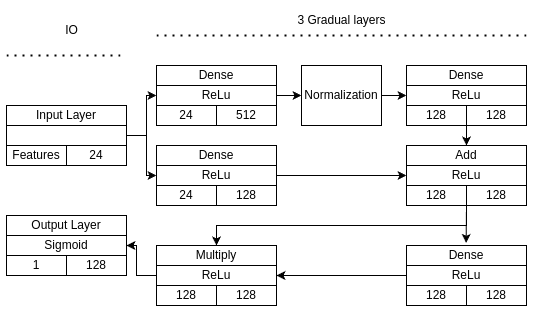
\includegraphics[width=0.8\textwidth]{obrazky-figures/tls_attention.png}
\caption{Architektura specializovaného TLS klasifikátoru s~feature-wise gatingem.}
\label{fig:tls_classifier_architecture}
\end{figure}

\section*{Výsledky klasifikace}
\label{appendix:tls-results}

Model \texttt{attention\_tls} byl testován ve třetí fázi klasifikace samostatně pro phishingové a malware domény. Na validační datové sadě dosahoval velmi vysoké výkonnosti – přesnost, úplnost i F1 skóre se pohybovaly nad 95~\%, jak shrnuje tabulka~\ref{tab:attention_tls_results}.


\begin{table}[h!]
    \centering
        \begin{tabular}{|l|c|c|}
            \hline
            \textbf{Metrika} & \textbf{Phishing} & \textbf{Malware} \\
            \hline
            Přesnost klasifikace (Accuracy)& 0{,}9934 ± 1{,}4e-04 & 0{,}9896 ± 7{,}8e-05 \\
            Přesnost pozitivní třídy (Precision)    & 0{,}9882 ± 8{,}8e-05 & 0{,}9660 ± 7{,}2e-05 \\
            Úplnost (Recall)        & 0{,}9722 ± 5{,}2e-05 & 0{,}9383 ± 5{,}7e-05 \\
            F1 skóre                & 0{,}9801 ± 6{,}4e-05 & 0{,}9519 ± 4{,}8e-05 \\
            ROC AUC                 & 0{,}9849 ± 7{,}9e-05 & 0{,}9671 ± 6{,}1e-05 \\
            \hline
        \end{tabular}
        \caption{Výsledky klasifikace modelu \texttt{tls} pro phishing a malware domény (10 běhů)}
    \label{tab:attention_tls_results}
\end{table}

Z~těchto výsledků vyplývá, že samotné TLS příznaky poskytují dostatečně bohatou informační hodnotu pro účinnou detekci škodlivých domén. Model vykazoval velmi vysoké hodnoty přesnosti, F1 skóre i AUC pro obě klasifikační úlohy a jeví se jako vhodný například pro nasazení v~prostředích s~omezeným přístupem k~DNS nebo aplikačním datům. Výsledky byly dále ověřeny na oddělené verifikační datové sadě, viz sekce \ref{verification_fail}.

\section*{Analýza matic záměn}

Kvalitu klasifikace potvrzuje i rozložení záměn zobrazené na obrázcích~\ref{fig:attention_tls_conf_matrix_phishing} a~\ref{fig:attention_tls_conf_matrix_malware}, kde je patrné minimum falešných pozitivních i negativních detekcí.

\begin{figure}[H]
    \centering
    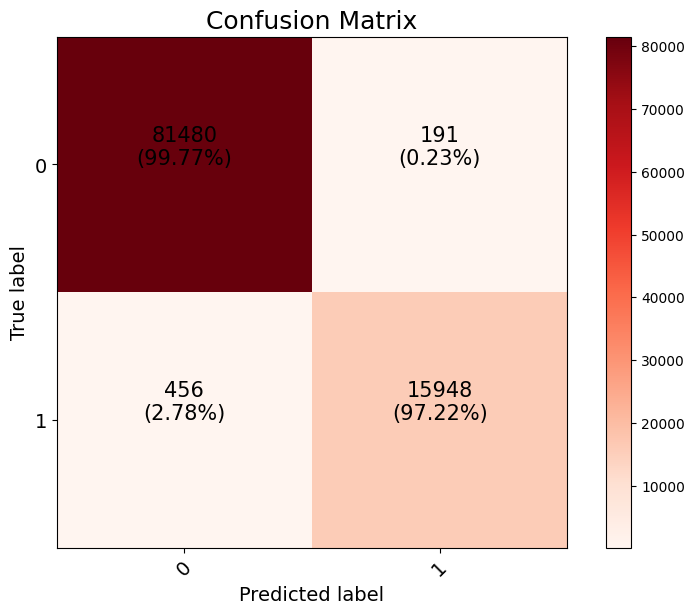
\includegraphics[width=0.8\textwidth]{obrazky-figures/attention_tls_stage_3_phishing_v1.1_confusion_matrix.png}
    \caption{Matice záměn pro phishingové domény (fáze~3).}
    \label{fig:attention_tls_conf_matrix_phishing}
\end{figure}

\begin{figure}[H]
    \centering
    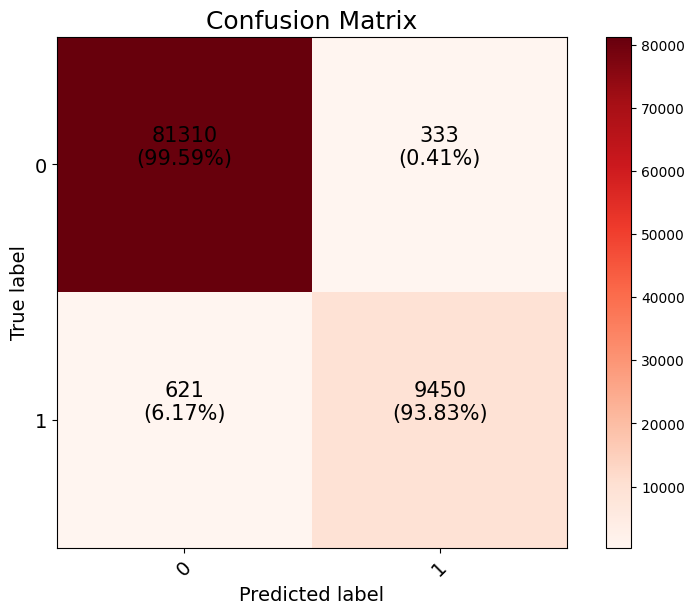
\includegraphics[width=0.8\textwidth]{obrazky-figures/attention_tls_stage_3_malware_v1.1_confusion_matrix.png}
    \caption{Matice záměn pro malware domény (fáze~3).}
    \label{fig:attention_tls_conf_matrix_malware}
\end{figure}

\section*{Výsledky na verifikační datové sadě}
\label{verification_fail}
Přestože model \texttt{attention\_tls} dosáhl velmi dobrých výsledků na validační datové sadě (viz Tabulka~\ref{tab:attention_tls_results}), jeho výkon na verifikačním vzorku byl výrazně slabší (viz Tabulka~\ref{tab:tls_attention_combined}) , zejména v~případě detekce malware domén. Zatímco recall zůstal vysoký, přesnost (precision) se u~obou úloh propadla, což naznačuje zvýšený počet falešně pozitivních klasifikací.

Z~důvodu této slabší generalizace nebyl model založený výhradně na TLS příznacích zapojen do výsledné klasifikační pipeline. Přesto však považujeme tento přístup za zajímavý směr dalšího výzkumu – zejména s~ohledem na nízké nároky na vstupní data a možnost jeho nasazení v~prostředích s~omezenými možnostmi hlubší inspekce.

\begin{table}[h!]
\centering
\begin{tabular}{|l|c|c|}
\hline
\textbf{Metrika} & \textbf{Malware} & \textbf{Phishing} \\
\hline
Přesnost klasifikace (Accuracy)      & \texttt{0.8750 ± 6.2e-05} & \texttt{0.9278 ± 4.8e-05} \\
Přesnost pozitivní třídy (Precision) & \texttt{0.5814 ± 1.1e-04} & \texttt{0.7072 ± 9.1e-05} \\
Úplnost (Recall)                     & \texttt{0.8117 ± 9.0e-05} & \texttt{0.9481 ± 9.3e-05} \\
F1 skóre                             & \texttt{0.6767 ± 5.8e-05} & \texttt{0.8101 ± 4.1e-05} \\
ROC AUC                              & \texttt{0.8573 ± 7.2e-05} & \texttt{0.9360 ± 7.0e-05} \\
\hline
\end{tabular}
\caption{Srovnání metrik modelu \texttt{attention\_tls} (Stage 3) pro malware a phishing (10 běhů).}
\label{tab:tls_attention_combined}
\end{table}

\section*{Závěr}

Specializovaný model \texttt{attention\_tls} ukázal, že je možné klasifikovat domény pouze na základě TLS metadat, bez nutnosti využití DNS, WHOIS nebo aplikačních příznaků. Při validaci dosáhl velmi dobrých výsledků a potvrdil, že TLS příznaky představují zajímavý, byť v~praxi dosud málo využívaný, zdroj informací pro detekci škodlivých domén.

Při testování na verifikační datové sadě se však ukázalo, že model nedosahuje stejné úrovně generalizace. Zatímco úplnost zůstala vysoká, přesnost poklesla, zejména v~případě malware domén, což vedlo ke zvýšenému výskytu falešně pozitivních klasifikací. Vzhledem k~těmto výsledkům nebyl model \texttt{attention\_tls} zařazen do finální klasifikační pipeline.

Přesto zůstává přístup založený na TLS a jeho samostatná klasifikace relevantní a slibnou oblastí pro další výzkum – zejména v~kontextu pasivního monitoringu, analýzy šifrovaného provozu a nasazení v~edge prostředích. Dále by bylo vhodné zkoumat možnosti rozšíření sady příznaků, robustnější trénovací přístupy a metody kombinace s~jinými modalitami pro zvýšení odolnosti vůči rozdílům v~distribuci dat mezi sadami.






\chapter{Výsledky analýzy SHAP}
\label{sec:appendix-shap}

Analýza Shapleyho hodnot (SHAP) poskytuje hlubší pohled na to, jak jednotlivé příznaky přispívají k~rozhodování konkrétních modelů. Následující grafy znázorňují distribuci hodnot SHAP pro každý model zvlášť.

\begin{figure}[!ht]
    \centering
    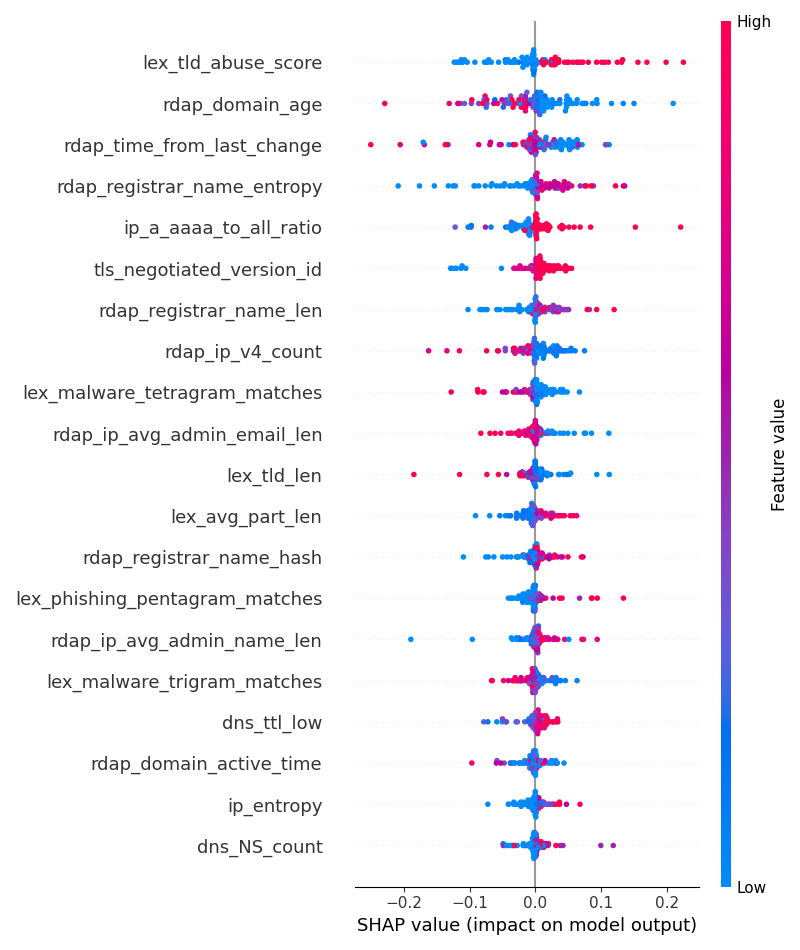
\includegraphics[width=1.0\textwidth]{obrazky-figures/shap_feedforward.png}
    \caption{Přínos jednotlivých příznaků pro model FFNN}
    \label{fig:shap_feedforward}
\end{figure}

Model FFNN klade největší důraz na příznaky z~oblasti RDAP  \texttt{rdap\_domain\_age}) a lexikálních znaků domény (např. \texttt{lex\_tld\_abuse\_score}). Dále je patrný vliv vybraných TLS atributů, i když jejich dopad je ve srovnání s~ostatními kategoriemi menší.

\begin{figure}[!ht]
    \centering
    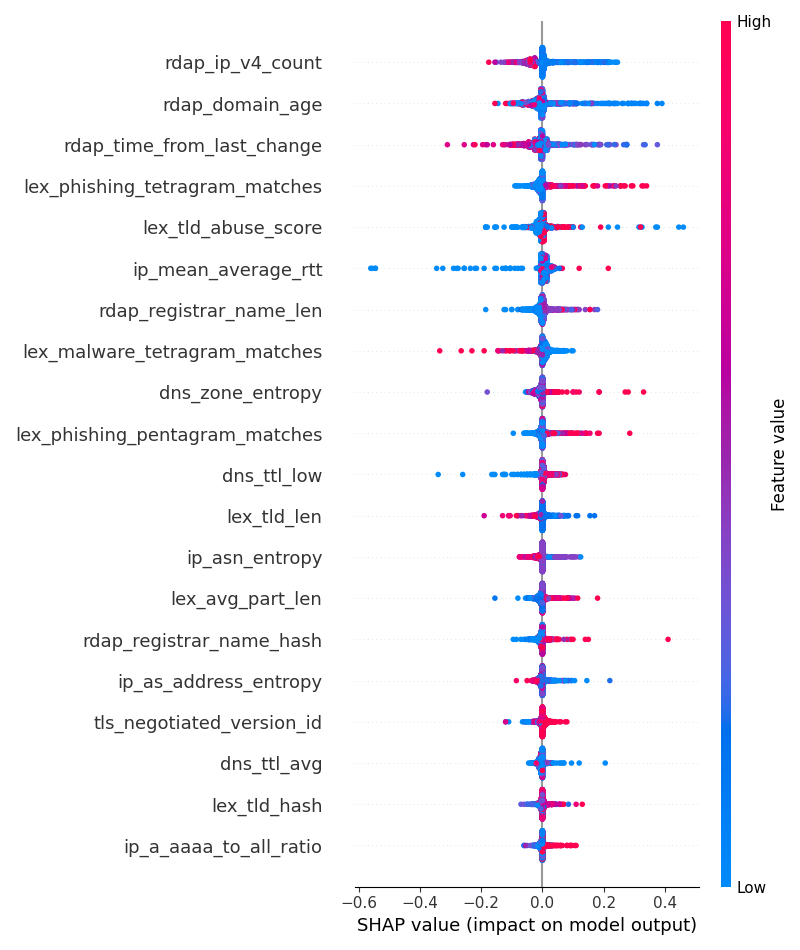
\includegraphics[width=1.0\textwidth]{obrazky-figures/shap_Lgbm.png}
    \caption{Přínos jednotlivých příznaků pro model LightGBM}
    \label{fig:shap_Lgbm}
\end{figure}

U~modelu LightGBM dominují atributy z~RDAP oblasti a DNS záznamy, přičemž příznak \texttt{rdap\_ip\_v4\_count} patří mezi nejvýznamnější. Rovněž se zde více uplatňuje informační entropie z~IP a DNS zón.

\begin{figure}[!ht]
    \centering
    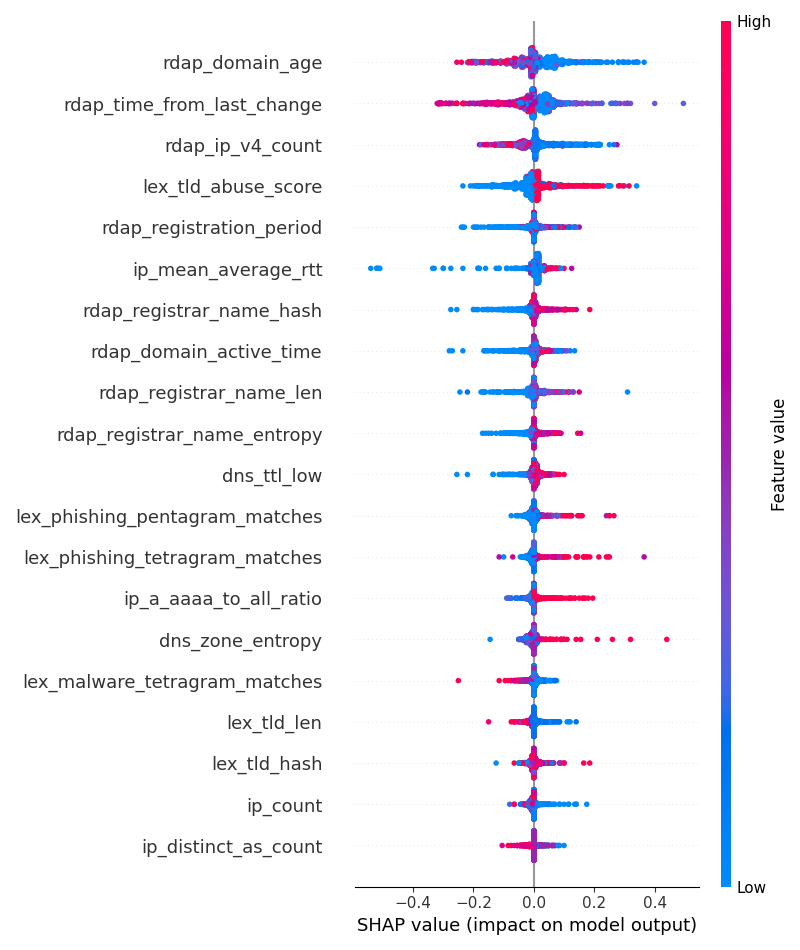
\includegraphics[width=1.0\textwidth]{obrazky-figures/shap_XgBoost.png}
    \caption{Přínos jednotlivých příznaků pro model XGBoost}
    \label{fig:shap_XgBoost}
\end{figure}

Model XGBoost se opírá o~podobné sady příznaků, nicméně více zvýrazňuje lexikální znaky druhé úrovně domény (např. \texttt{lex\_sld\_digit\_count}) a specifické TLS vlastnosti jako \texttt{tls\_CA\_certs\_in\_chain\_ratio}. Příznaky z~RDAP oblasti zůstávají důležitým základem.

\begin{figure}[!ht]
    \centering
    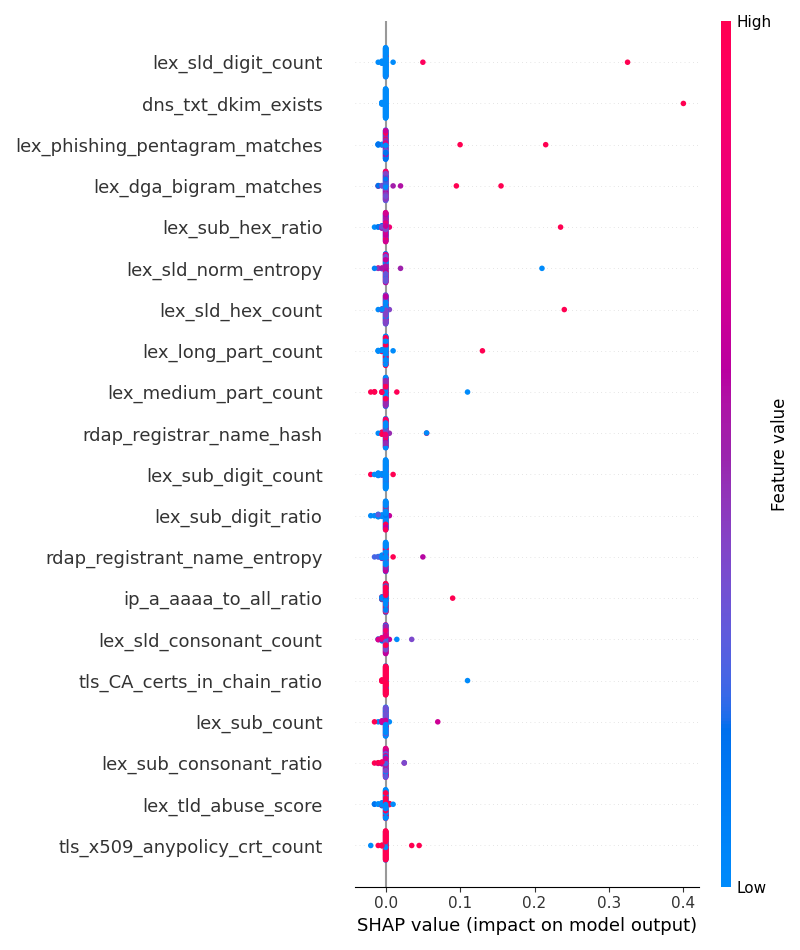
\includegraphics[width=1.0\textwidth]{obrazky-figures/shap_svm.png}
    \caption{Přínos jednotlivých příznaků pro model SVM}
    \label{fig:shap_svm}
\end{figure}

SVM model rovněž ukazuje silnou závislost na RDAP příznacích (věk domény, délka registrace), doplněnou o~lexikální charakteristiky a síťové vlastnosti. Model reflektuje robustní schopnost klasifikace při kombinaci více typů příznaků.

\section*{Přínos všech příznaků napříč modely}

Kromě pohledu na jednotlivé modely byla provedena agregovaná analýza SHAP hodnot napříč celou klasifikační pipeline.

\begin{figure}[!ht]
    \centering
    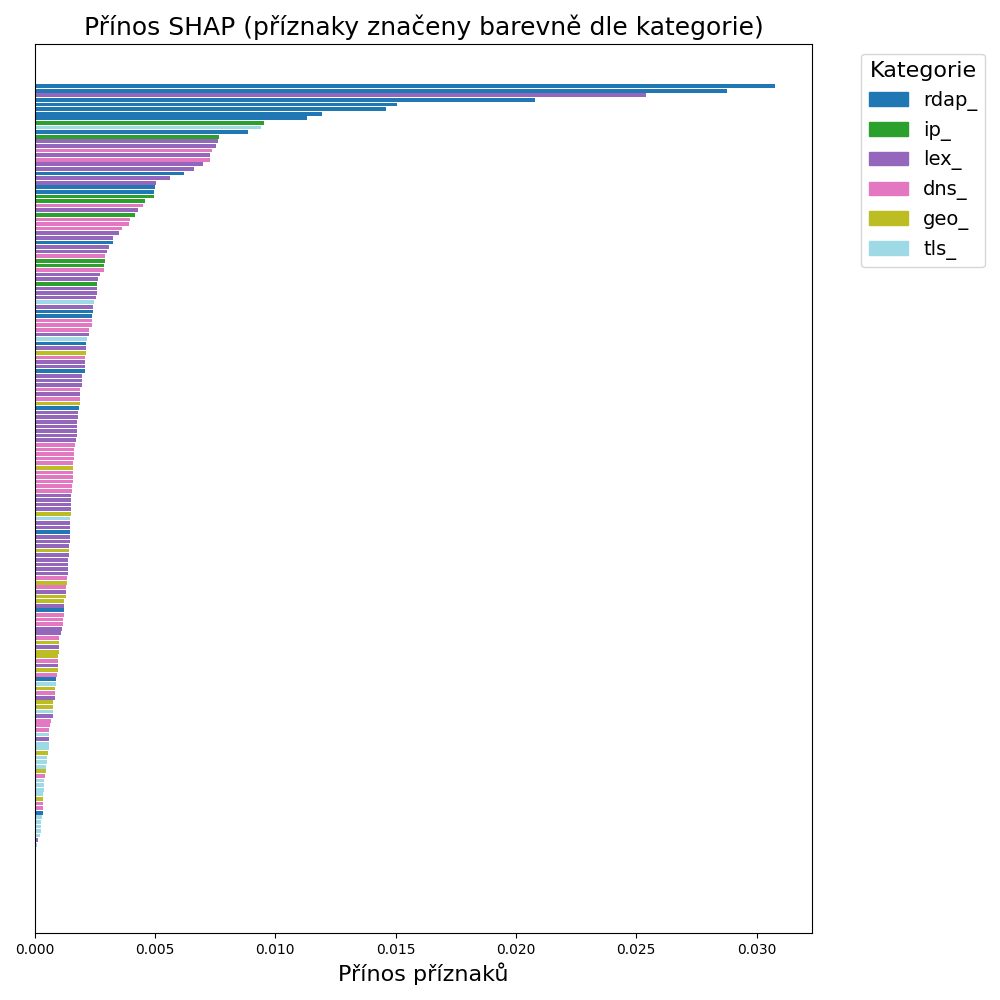
\includegraphics[width=1.0\textwidth]{obrazky-figures/all_shap.png}
    \caption{Průměrný SHAP přínos všech příznaků, barevně rozlišen dle kategorií}
    \label{fig:all_shap}
\end{figure}

Na obrázku \ref{fig:all_shap} jsou jednotlivé příznaky seřazeny dle jejich průměrného přínosu k~rozhodování. Dominují především příznaky z~RDAP oblasti, následované IP a lexikálními znaky. Barevné označení umožňuje sledovat, které kategorie přispívají nejvíce, a zároveň ukazuje značný pokles důležitosti u~DNS, GEO a TLS příznaků.

\begin{figure}[!ht]
    \centering
    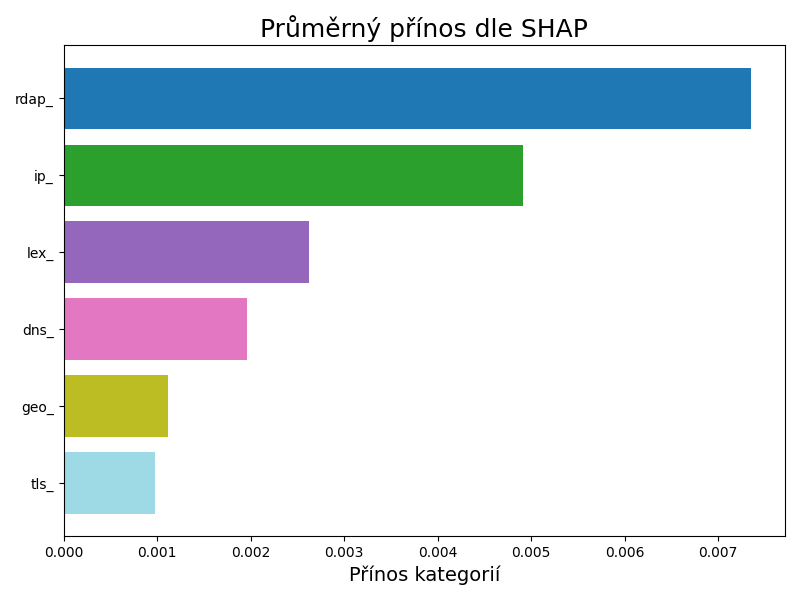
\includegraphics[width=0.8\textwidth]{obrazky-figures/shap_cat.png}
    \caption{Průměrný přínos příznaků dle kategorií}
    \label{fig:shap_cat}
\end{figure}

Konečný souhrn na obrázku \ref{fig:shap_cat} kvantifikuje průměrný přínos jednotlivých kategorií. Nejvyšší přínos vykazují RDAP příznaky, následované IP a lexikálními znaky domény. Naopak TLS a GEO atributy měly relativně nízký vliv, což naznačuje jejich omezenou roli v~celkové klasifikaci. Tyto poznatky mohou být vodítkem pro budoucí redukci dimenze nebo návrh specializovaných klasifikátorů pro jednotlivé kategorie.










\chapter{Měření klasifikace dle podmnožin}
\label{sec:appendix-results}

Tato příloha obsahuje kompletní výsledky všech měření samostatných i agregovaných subsetů příznaků pro klasifikaci phishingových a malware domén.

Každý výstup zobrazuje přesnost jednotlivých klasifikačních algoritmů na dané kombinaci příznaků, zvlášť pro phishing a zvlášť pro malware. Měření byla provedena podle metodologie popsané v~kapitole \textbf{Předběžná analýza podmnožin příznaků}, kde byl popsán postup automatizovaného trénování modelů pomocí knihovny \texttt{PyCaret}. Cílem bylo identifikovat optimální kombinace atributů a klasifikátorů pro detekci škodlivých domén.

\subsection*{Použité klasifikátory}

Následující tabulka obsahuje zkratky používané v~jednotlivých výstupech a jejich odpovídající plné názvy modelů. Tyto zkratky byly zvoleny pro zajištění přehlednosti a úsporu místa ve výstupech.

\begin{table}[H]
    \centering
    \caption{Zkratky použitých klasifikátorů}
    \label{tab:model_abbreviations}
    \begin{tabular}{|l|l|l|}
        \hline
        \textbf{Zkratka} & \textbf{Plný název} & \textbf{Poznámka} \\
        \hline
        \texttt{RF} & Random Forest Classifier & Ensemble \\
        \texttt{ADA} & Ada Boost Classifier & Ensemble \\
        \texttt{DT} & Decision Tree Classifier & Interpretable \\
        \texttt{Ridge} & Ridge Classifier & Linear model \\
        \texttt{KNN} & K~Neighbors Classifier & Instance-based \\
        \texttt{SVM-L} & SVM - Linear Kernel & Linear SVM \\
        \texttt{LR} & Logistic Regression & Linear model \\
        \texttt{QDA} & Quadratic Discriminant Analysis & Probabilistic \\
        \texttt{NB} & Naive Bayes & Probabilistic \\
        \texttt{ET} & Extra Trees Classifier & Ensemble \\
        \texttt{XGB} & Extreme Gradient Boosting & Boosted Trees \\
        \texttt{LGBM} & Light Gradient Boosting Machine & Boosted Trees \\
        \texttt{GBC} & Gradient Boosting Classifier & Boosted Trees \\
        \texttt{LDA} & Linear Discriminant Analysis & Probabilistic \\
        \texttt{Dummy} & Dummy Classifier & Referenční baseline \\
        \hline
    \end{tabular}
\end{table}

\subsection*{Komentář k~výstupům}

Každá tabulka představuje výsledky pro konkrétní subset příznaků a typ útoku (phishing nebo malware).  
Metody jsou porovnávány dle hlavních metrik klasifikace: přesnost (\textbf{Acc}), plocha pod ROC křivkou (\textbf{AUC}), \textbf{Recall}, \textbf{Precision}, \textbf{F1 skóre}, Cohenova \textbf{Kappa} a \textbf{Matthews Correlation Coefficient} (MCC).

Díky oddělení výsledků pro phishing a malware je možné detailně porovnat účinnost jednotlivých přístupů pro různé typy útoků a rozhodnout o~vhodné strategii nasazení.

\bigskip

\begin{table}[H]
  \centering
  \small
  \caption{Výsledky pro subset dns – malware}
  \begin{tabular}{|l|c|c|c|c|c|c|c|c|}
    \hline
    \textbf{Model} & \textbf{Acc} & \textbf{AUC} & \textbf{Recall} & \textbf{Prec.} & \textbf{F1} & \textbf{Kappa} & \textbf{MCC} & \textbf{TT (s)} \\
    \hline
    Random Forest Classifier & 0.9165 & 0.9120 & 0.9165 & 0.9135 & 0.9143 & 0.6861 & 0.6886 & 1.80 \\
    Extra Trees Classifier & 0.9155 & 0.8910 & 0.9155 & 0.9125 & 0.9133 & 0.6829 & 0.6851 & 0.45 \\
    K Neighbors Classifier & 0.9142 & 0.8860 & 0.9142 & 0.9109 & 0.9116 & 0.6757 & 0.6787 & 0.24 \\
    Extreme Gradient Boosting & 0.9166 & 0.9175 & 0.9166 & 0.9129 & 0.9115 & 0.6681 & 0.6785 & 0.44 \\
    Light Gradient Boosting Machine & 0.9174 & 0.9176 & 0.9174 & 0.9144 & 0.9113 & 0.6647 & 0.6794 & 0.61 \\
    Decision Tree Classifier & 0.8958 & 0.8503 & 0.8958 & 0.8957 & 0.8957 & 0.6268 & 0.6271 & 0.19 \\
    Gradient Boosting Classifier & 0.8911 & 0.8799 & 0.8911 & 0.8921 & 0.8728 & 0.4991 & 0.5538 & 2.77 \\
    Ada Boost Classifier & 0.8632 & 0.8417 & 0.8632 & 0.8536 & 0.8335 & 0.3352 & 0.3997 & 0.71 \\
    Linear Discriminant Analysis & 0.8491 & 0.7843 & 0.8491 & 0.8264 & 0.8136 & 0.2532 & 0.3100 & 0.17 \\
    Ridge Classifier & 0.8346 & 0.7842 & 0.8346 & 0.7962 & 0.7724 & 0.0722 & 0.1401 & 0.12 \\
    Logistic Regression & 0.8242 & 0.6988 & 0.8242 & 0.7307 & 0.7582 & 0.0143 & 0.0262 & 1.31 \\
    Dummy Classifier & 0.8317 & 0.5000 & 0.8317 & 0.6917 & 0.7553 & 0.0000 & 0.0000 & 0.06 \\
    SVM - Linear Kernel & 0.6466 & 0.6454 & 0.6466 & 0.7720 & 0.6756 & 0.1180 & 0.1475 & 0.14 \\
    Quadratic Discriminant Analysis & 0.5847 & 0.7880 & 0.5847 & 0.8468 & 0.6332 & 0.2208 & 0.3161 & 0.14 \\
    Naive Bayes & 0.3432 & 0.6313 & 0.3432 & 0.8202 & 0.3546 & 0.0640 & 0.1513 & 0.07 \\
    \hline
  \end{tabular}
\end{table}
\vspace{0.5cm}

\begin{table}[H]
  \centering
  \small
  \caption{Výsledky pro subset geo – malware}
  \begin{tabular}{|l|c|c|c|c|c|c|c|c|}
    \hline
    \textbf{Model} & \textbf{Acc} & \textbf{AUC} & \textbf{Recall} & \textbf{Prec.} & \textbf{F1} & \textbf{Kappa} & \textbf{MCC} & \textbf{TT (s)} \\
    \hline
    Random Forest Classifier & 0.8461 & 0.8194 & 0.8461 & 0.8210 & 0.8106 & 0.2416 & 0.2948 & 0.28 \\
    Extra Trees Classifier & 0.8461 & 0.8173 & 0.8461 & 0.8210 & 0.8102 & 0.2400 & 0.2939 & 0.25 \\
    Light Gradient Boosting Machine & 0.8482 & 0.8291 & 0.8482 & 0.8272 & 0.8098 & 0.2352 & 0.2998 & 0.62 \\
    Decision Tree Classifier & 0.8446 & 0.8161 & 0.8446 & 0.8176 & 0.8092 & 0.2367 & 0.2870 & 0.13 \\
    Extreme Gradient Boosting & 0.8474 & 0.8277 & 0.8474 & 0.8249 & 0.8092 & 0.2333 & 0.2953 & 0.22 \\
    K Neighbors Classifier & 0.8380 & 0.7701 & 0.8380 & 0.8056 & 0.8031 & 0.2147 & 0.2555 & 0.15 \\
    Gradient Boosting Classifier & 0.8446 & 0.8170 & 0.8446 & 0.8218 & 0.8000 & 0.1915 & 0.2634 & 2.24 \\
    Ada Boost Classifier & 0.8342 & 0.7980 & 0.8342 & 0.7815 & 0.7674 & 0.0511 & 0.1055 & 0.63 \\
    Ridge Classifier & 0.8317 & 0.6927 & 0.8317 & 0.6917 & 0.7553 & -0.0001 & -0.0010 & 0.10 \\
    Linear Discriminant Analysis & 0.8317 & 0.6928 & 0.8317 & 0.6917 & 0.7553 & -0.0001 & -0.0010 & 0.13 \\
    Dummy Classifier & 0.8317 & 0.5000 & 0.8317 & 0.6917 & 0.7553 & 0.0000 & 0.0000 & 0.06 \\
    Logistic Regression & 0.8311 & 0.7075 & 0.8311 & 0.7085 & 0.7551 & -0.0008 & -0.0044 & 1.28 \\
    SVM - Linear Kernel & 0.7870 & 0.5542 & 0.7870 & 0.7089 & 0.7393 & 0.0064 & 0.0019 & 0.13 \\
    Quadratic Discriminant Analysis & 0.4123 & 0.7363 & 0.4123 & 0.8469 & 0.4425 & 0.1110 & 0.2242 & 0.11 \\
    Naive Bayes & 0.3427 & 0.6407 & 0.3427 & 0.7833 & 0.3620 & 0.0453 & 0.1011 & 0.06 \\
    \hline
  \end{tabular}
\end{table}
\vspace{0.5cm}

\begin{table}[H]
  \centering
  \small
  \caption{Výsledky pro subset html – malware}
  \begin{tabular}{|l|c|c|c|c|c|c|c|c|}
    \hline
    \textbf{Model} & \textbf{Acc} & \textbf{AUC} & \textbf{Recall} & \textbf{Prec.} & \textbf{F1} & \textbf{Kappa} & \textbf{MCC} & \textbf{TT (s)} \\
    \hline
    Random Forest Classifier & 0.8410 & 0.7060 & 0.8410 & 0.8313 & 0.7824 & 0.1133 & 0.2110 & 0.38 \\
    Light Gradient Boosting Machine & 0.8414 & 0.7098 & 0.8414 & 0.8357 & 0.7823 & 0.1127 & 0.2145 & 1.20 \\
    Extreme Gradient Boosting & 0.8411 & 0.7090 & 0.8411 & 0.8327 & 0.7822 & 0.1125 & 0.2115 & 0.34 \\
    Extra Trees Classifier & 0.8403 & 0.7009 & 0.8403 & 0.8260 & 0.7820 & 0.1117 & 0.2046 & 0.31 \\
    K Neighbors Classifier & 0.8409 & 0.6828 & 0.8409 & 0.8346 & 0.7811 & 0.1075 & 0.2087 & 0.21 \\
    Gradient Boosting Classifier & 0.8416 & 0.7078 & 0.8416 & 0.8485 & 0.7804 & 0.1041 & 0.2174 & 4.35 \\
    Ada Boost Classifier & 0.8411 & 0.6954 & 0.8411 & 0.8476 & 0.7793 & 0.0995 & 0.2111 & 1.20 \\
    Decision Tree Classifier & 0.8285 & 0.6875 & 0.8285 & 0.7733 & 0.7745 & 0.0854 & 0.1272 & 0.28 \\
    Logistic Regression & 0.8313 & 0.6499 & 0.8313 & 0.7142 & 0.7553 & -0.0000 & 0.0011 & 1.73 \\
    Dummy Classifier & 0.8317 & 0.5000 & 0.8317 & 0.6917 & 0.7553 & 0.0000 & 0.0000 & 0.08 \\
    Ridge Classifier & 0.8315 & 0.6633 & 0.8315 & 0.6917 & 0.7552 & -0.0004 & -0.0034 & 0.16 \\
    Linear Discriminant Analysis & 0.8314 & 0.6617 & 0.8314 & 0.6917 & 0.7551 & -0.0007 & -0.0063 & 0.29 \\
    SVM - Linear Kernel & 0.7869 & 0.6562 & 0.7869 & 0.7278 & 0.7350 & 0.0172 & 0.0288 & 0.24 \\
    Naive Bayes & 0.4640 & 0.6623 & 0.4640 & 0.8337 & 0.5074 & 0.1309 & 0.2305 & 0.09 \\
    Quadratic Discriminant Analysis & 0.4459 & 0.6664 & 0.4459 & 0.8477 & 0.4837 & 0.1304 & 0.2437 & 0.20 \\
    \hline
  \end{tabular}
\end{table}
\vspace{0.5cm}

\begin{table}[H]
  \centering
  \small
  \caption{Výsledky pro subset ip – malware}
  \begin{tabular}{|l|c|c|c|c|c|c|c|c|}
    \hline
    \textbf{Model} & \textbf{Acc} & \textbf{AUC} & \textbf{Recall} & \textbf{Prec.} & \textbf{F1} & \textbf{Kappa} & \textbf{MCC} & \textbf{TT (s)} \\
    \hline
    Extreme Gradient Boosting & 0.8669 & 0.8812 & 0.8669 & 0.8524 & 0.8511 & 0.4242 & 0.4478 & 0.22 \\
    Light Gradient Boosting Machine & 0.8669 & 0.8817 & 0.8669 & 0.8524 & 0.8490 & 0.4124 & 0.4414 & 0.59 \\
    K Neighbors Classifier & 0.8553 & 0.8210 & 0.8553 & 0.8452 & 0.8469 & 0.4289 & 0.4379 & 0.20 \\
    Random Forest Classifier & 0.8437 & 0.8314 & 0.8437 & 0.8312 & 0.8359 & 0.3888 & 0.3930 & 0.32 \\
    Extra Trees Classifier & 0.8425 & 0.7755 & 0.8425 & 0.8296 & 0.8343 & 0.3824 & 0.3868 & 0.35 \\
    Gradient Boosting Classifier & 0.8589 & 0.8582 & 0.8589 & 0.8421 & 0.8326 & 0.3372 & 0.3833 & 1.13 \\
    Decision Tree Classifier & 0.8406 & 0.7284 & 0.8406 & 0.8273 & 0.8322 & 0.3740 & 0.3786 & 0.10 \\
    Ada Boost Classifier & 0.8404 & 0.8359 & 0.8404 & 0.8126 & 0.7911 & 0.1533 & 0.2249 & 0.39 \\
    Linear Discriminant Analysis & 0.8317 & 0.7536 & 0.8317 & 0.7283 & 0.7556 & 0.0015 & 0.0107 & 0.12 \\
    Ridge Classifier & 0.8317 & 0.7537 & 0.8317 & 0.6917 & 0.7553 & -0.0001 & -0.0010 & 0.10 \\
    Dummy Classifier & 0.8317 & 0.5000 & 0.8317 & 0.6917 & 0.7553 & 0.0000 & 0.0000 & 0.06 \\
    Logistic Regression & 0.8306 & 0.7597 & 0.8306 & 0.7085 & 0.7551 & -0.0007 & -0.0047 & 0.38 \\
    SVM - Linear Kernel & 0.7730 & 0.6588 & 0.7730 & 0.7781 & 0.7467 & 0.1158 & 0.1512 & 0.18 \\
    Quadratic Discriminant Analysis & 0.5441 & 0.7503 & 0.5441 & 0.8516 & 0.5921 & 0.1961 & 0.3035 & 0.10 \\
    Naive Bayes & 0.5152 & 0.6785 & 0.5152 & 0.8361 & 0.5638 & 0.1630 & 0.2599 & 0.06 \\
    \hline
  \end{tabular}
\end{table}
\vspace{0.5cm}

\begin{table}[H]
  \centering
  \small
  \caption{Výsledky pro subset lex – malware}
  \begin{tabular}{|l|c|c|c|c|c|c|c|c|}
    \hline
    \textbf{Model} & \textbf{Acc} & \textbf{AUC} & \textbf{Recall} & \textbf{Prec.} & \textbf{F1} & \textbf{Kappa} & \textbf{MCC} & \textbf{TT (s)} \\
    \hline
    Light Gradient Boosting Machine & 0.9371 & 0.9352 & 0.9371 & 0.9358 & 0.9338 & 0.7531 & 0.7618 & 0.69 \\
    Extreme Gradient Boosting & 0.9341 & 0.9303 & 0.9341 & 0.9321 & 0.9311 & 0.7441 & 0.7507 & 0.33 \\
    Gradient Boosting Classifier & 0.9255 & 0.9204 & 0.9255 & 0.9248 & 0.9194 & 0.6940 & 0.7125 & 5.58 \\
    Random Forest Classifier & 0.9238 & 0.9144 & 0.9238 & 0.9215 & 0.9188 & 0.6944 & 0.7068 & 0.44 \\
    Extra Trees Classifier & 0.9213 & 0.8860 & 0.9213 & 0.9187 & 0.9158 & 0.6824 & 0.6959 & 0.50 \\
    Ada Boost Classifier & 0.9066 & 0.8994 & 0.9066 & 0.9018 & 0.8989 & 0.6161 & 0.6325 & 1.28 \\
    Linear Discriminant Analysis & 0.8987 & 0.8850 & 0.8987 & 0.8952 & 0.8864 & 0.5604 & 0.5920 & 0.23 \\
    Decision Tree Classifier & 0.8761 & 0.7909 & 0.8761 & 0.8780 & 0.8769 & 0.5637 & 0.5639 & 0.38 \\
    Ridge Classifier & 0.8929 & 0.8852 & 0.8929 & 0.8945 & 0.8751 & 0.5083 & 0.5627 & 0.12 \\
    K Neighbors Classifier & 0.8635 & 0.7860 & 0.8635 & 0.8479 & 0.8475 & 0.4106 & 0.4329 & 0.20 \\
    Logistic Regression & 0.8317 & 0.4768 & 0.8317 & 0.6917 & 0.7553 & 0.0000 & 0.0000 & 0.17 \\
    Naive Bayes & 0.8317 & 0.5302 & 0.8317 & 0.6917 & 0.7553 & 0.0000 & 0.0000 & 0.08 \\
    SVM - Linear Kernel & 0.8317 & 0.4927 & 0.8317 & 0.6917 & 0.7553 & 0.0000 & 0.0000 & 0.63 \\
    Dummy Classifier & 0.8317 & 0.5000 & 0.8317 & 0.6917 & 0.7553 & 0.0000 & 0.0000 & 0.07 \\
    Quadratic Discriminant Analysis & 0.3245 & 0.8671 & 0.3245 & 0.8487 & 0.3192 & 0.0676 & 0.1740 & 0.15 \\
    \hline
  \end{tabular}
\end{table}
\vspace{0.5cm}

\begin{table}[H]
  \centering
  \small
  \caption{Výsledky pro subset rdap – malware}
  \begin{tabular}{|l|c|c|c|c|c|c|c|c|}
    \hline
    \textbf{Model} & \textbf{Acc} & \textbf{AUC} & \textbf{Recall} & \textbf{Prec.} & \textbf{F1} & \textbf{Kappa} & \textbf{MCC} & \textbf{TT (s)} \\
    \hline
    Light Gradient Boosting Machine & 0.9533 & 0.9590 & 0.9533 & 0.9524 & 0.9518 & 0.8228 & 0.8265 & 0.64 \\
    Extreme Gradient Boosting & 0.9522 & 0.9589 & 0.9522 & 0.9512 & 0.9509 & 0.8204 & 0.8230 & 0.35 \\
    Random Forest Classifier & 0.9502 & 0.9572 & 0.9502 & 0.9491 & 0.9487 & 0.8121 & 0.8151 & 0.33 \\
    Extra Trees Classifier & 0.9467 & 0.9410 & 0.9467 & 0.9455 & 0.9450 & 0.7980 & 0.8016 & 0.33 \\
    Gradient Boosting Classifier & 0.9358 & 0.9420 & 0.9358 & 0.9342 & 0.9326 & 0.7489 & 0.7568 & 3.20 \\
    Decision Tree Classifier & 0.9319 & 0.8981 & 0.9319 & 0.9313 & 0.9315 & 0.7541 & 0.7543 & 0.19 \\
    K Neighbors Classifier & 0.9296 & 0.8997 & 0.9296 & 0.9275 & 0.9281 & 0.7381 & 0.7396 & 0.17 \\
    Ada Boost Classifier & 0.9196 & 0.9229 & 0.9196 & 0.9160 & 0.9159 & 0.6877 & 0.6938 & 0.81 \\
    Linear Discriminant Analysis & 0.8576 & 0.8538 & 0.8576 & 0.8402 & 0.8421 & 0.3919 & 0.4102 & 0.14 \\
    Ridge Classifier & 0.8476 & 0.8539 & 0.8476 & 0.8271 & 0.8067 & 0.2207 & 0.2905 & 0.11 \\
    Naive Bayes & 0.8317 & 0.7152 & 0.8317 & 0.6917 & 0.7553 & 0.0000 & 0.0000 & 0.07 \\
    Dummy Classifier & 0.8317 & 0.5000 & 0.8317 & 0.6917 & 0.7553 & 0.0000 & 0.0000 & 0.06 \\
    Logistic Regression & 0.6944 & 0.4346 & 0.6944 & 0.6868 & 0.6857 & -0.0985 & -0.1081 & 0.16 \\
    Quadratic Discriminant Analysis & 0.6038 & 0.8827 & 0.6038 & 0.8596 & 0.6506 & 0.2492 & 0.3524 & 0.12 \\
    SVM - Linear Kernel & 0.4393 & 0.4665 & 0.4393 & 0.6703 & 0.4658 & -0.1430 & -0.1609 & 0.36 \\
    \hline
  \end{tabular}
\end{table}
\vspace{0.5cm}

\begin{table}[H]
  \centering
  \small
  \caption{Výsledky pro subset tls – malware}
  \begin{tabular}{|l|c|c|c|c|c|c|c|c|}
    \hline
    \textbf{Model} & \textbf{Acc} & \textbf{AUC} & \textbf{Recall} & \textbf{Prec.} & \textbf{F1} & \textbf{Kappa} & \textbf{MCC} & \textbf{TT (s)} \\
    \hline
    Decision Tree Classifier & 0.8370 & 0.6894 & 0.8370 & 0.8323 & 0.7706 & 0.0633 & 0.1591 & 0.07 \\
    Random Forest Classifier & 0.8373 & 0.6889 & 0.8373 & 0.8393 & 0.7705 & 0.0629 & 0.1633 & 0.21 \\
    Extra Trees Classifier & 0.8371 & 0.6887 & 0.8371 & 0.8362 & 0.7705 & 0.0629 & 0.1612 & 0.23 \\
    Extreme Gradient Boosting & 0.8370 & 0.6919 & 0.8370 & 0.8360 & 0.7703 & 0.0620 & 0.1600 & 0.28 \\
    Light Gradient Boosting Machine & 0.8369 & 0.6885 & 0.8369 & 0.8346 & 0.7701 & 0.0613 & 0.1580 & 0.49 \\
    Gradient Boosting Classifier & 0.8366 & 0.6848 & 0.8366 & 0.8371 & 0.7689 & 0.0562 & 0.1531 & 0.56 \\
    Ada Boost Classifier & 0.8356 & 0.6326 & 0.8356 & 0.8327 & 0.7670 & 0.0482 & 0.1385 & 0.28 \\
    Ridge Classifier & 0.8349 & 0.6280 & 0.8349 & 0.8172 & 0.7667 & 0.0473 & 0.1275 & 0.12 \\
    Linear Discriminant Analysis & 0.8330 & 0.6279 & 0.8330 & 0.7916 & 0.7665 & 0.0469 & 0.1093 & 0.14 \\
    K Neighbors Classifier & 0.8342 & 0.5444 & 0.8342 & 0.8192 & 0.7641 & 0.0364 & 0.1129 & 0.15 \\
    Naive Bayes & 0.8280 & 0.5668 & 0.8280 & 0.7525 & 0.7608 & 0.0239 & 0.0522 & 0.06 \\
    Dummy Classifier & 0.8317 & 0.5000 & 0.8317 & 0.6917 & 0.7553 & 0.0000 & 0.0000 & 0.06 \\
    Logistic Regression & 0.7481 & 0.5816 & 0.7481 & 0.7399 & 0.7438 & 0.0706 & 0.0707 & 0.15 \\
    SVM - Linear Kernel & 0.6982 & 0.5314 & 0.6982 & 0.7315 & 0.6935 & 0.0594 & 0.0544 & 0.31 \\
    Quadratic Discriminant Analysis & 0.6663 & 0.5838 & 0.6663 & 0.7567 & 0.6503 & 0.0769 & 0.0889 & 0.12 \\
    \hline
  \end{tabular}
\end{table}
\vspace{0.5cm}

\begin{table}[H]
  \centering
  \small
  \caption{Výsledky pro subset dns+rdap+tls+geo+ip+html+lex – malware}
  \begin{tabular}{|l|c|c|c|c|c|c|c|c|}
    \hline
    \textbf{Model} & \textbf{Acc} & \textbf{AUC} & \textbf{Recall} & \textbf{Prec.} & \textbf{F1} & \textbf{Kappa} & \textbf{MCC} & \textbf{TT (s)} \\
    \hline
    Light Gradient Boosting Machine & 0.9975 & 0.9999 & 0.9975 & 0.9975 & 0.9975 & 0.9874 & 0.9874 & 1.90 \\
    Extreme Gradient Boosting & 0.9974 & 0.9999 & 0.9974 & 0.9974 & 0.9974 & 0.9868 & 0.9868 & 4.62 \\
    Gradient Boosting Classifier & 0.9951 & 0.9997 & 0.9951 & 0.9951 & 0.9951 & 0.9752 & 0.9752 & 62.63 \\
    Ada Boost Classifier & 0.9945 & 0.9996 & 0.9945 & 0.9945 & 0.9945 & 0.9719 & 0.9719 & 14.63 \\
    Random Forest Classifier & 0.9942 & 0.9996 & 0.9942 & 0.9942 & 0.9941 & 0.9697 & 0.9699 & 2.64 \\
    Decision Tree Classifier & 0.9930 & 0.9829 & 0.9930 & 0.9930 & 0.9930 & 0.9643 & 0.9644 & 1.43 \\
    Extra Trees Classifier & 0.9888 & 0.9985 & 0.9888 & 0.9888 & 0.9885 & 0.9402 & 0.9415 & 3.27 \\
    Linear Discriminant Analysis & 0.9817 & 0.9958 & 0.9817 & 0.9817 & 0.9817 & 0.9063 & 0.9063 & 2.40 \\
    Ridge Classifier & 0.9774 & 0.9958 & 0.9774 & 0.9770 & 0.9767 & 0.8775 & 0.8801 & 0.71 \\
    K Neighbors Classifier & 0.9530 & 0.9313 & 0.9530 & 0.9512 & 0.9517 & 0.7471 & 0.7488 & 2.13 \\
    Logistic Regression & 0.9265 & 0.9632 & 0.9265 & 0.9228 & 0.9242 & 0.6016 & 0.6035 & 16.57 \\
    Dummy Classifier & 0.8901 & 0.5000 & 0.8901 & 0.7923 & 0.8384 & 0.0000 & 0.0000 & 0.47 \\
    SVM - Linear Kernel & 0.8355 & 0.6441 & 0.8355 & 0.8080 & 0.8110 & 0.0235 & 0.0326 & 7.67 \\
    Quadratic Discriminant Analysis & 0.7671 & 0.9591 & 0.7671 & 0.9177 & 0.8090 & 0.3690 & 0.4622 & 1.91 \\
    Naive Bayes & 0.6445 & 0.9416 & 0.6445 & 0.9136 & 0.7097 & 0.2464 & 0.3704 & 0.69 \\
    \hline
  \end{tabular}
\end{table}
\vspace{0.5cm}

\begin{table}[H]
  \centering
  \small
  \caption{Výsledky pro subset dns+rdap – malware}
  \begin{tabular}{|l|c|c|c|c|c|c|c|c|}
    \hline
    \textbf{Model} & \textbf{Acc} & \textbf{AUC} & \textbf{Recall} & \textbf{Prec.} & \textbf{F1} & \textbf{Kappa} & \textbf{MCC} & \textbf{TT (s)} \\
    \hline
    Light Gradient Boosting Machine & 0.9897 & 0.9989 & 0.9897 & 0.9898 & 0.9897 & 0.9478 & 0.9478 & 0.87 \\
    Extreme Gradient Boosting & 0.9895 & 0.9989 & 0.9895 & 0.9895 & 0.9895 & 0.9465 & 0.9465 & 1.25 \\
    Random Forest Classifier & 0.9878 & 0.9973 & 0.9878 & 0.9877 & 0.9878 & 0.9370 & 0.9371 & 1.08 \\
    Extra Trees Classifier & 0.9847 & 0.9933 & 0.9847 & 0.9845 & 0.9844 & 0.9192 & 0.9200 & 1.01 \\
    Decision Tree Classifier & 0.9826 & 0.9564 & 0.9826 & 0.9827 & 0.9827 & 0.9114 & 0.9114 & 0.44 \\
    Gradient Boosting Classifier & 0.9825 & 0.9971 & 0.9825 & 0.9826 & 0.9826 & 0.9109 & 0.9109 & 18.98 \\
    Ada Boost Classifier & 0.9800 & 0.9965 & 0.9800 & 0.9803 & 0.9801 & 0.8989 & 0.8990 & 4.46 \\
    Linear Discriminant Analysis & 0.9519 & 0.9794 & 0.9519 & 0.9520 & 0.9519 & 0.7547 & 0.7547 & 0.69 \\
    K Neighbors Classifier & 0.9423 & 0.9239 & 0.9423 & 0.9404 & 0.9411 & 0.6933 & 0.6943 & 1.04 \\
    Ridge Classifier & 0.9407 & 0.9794 & 0.9407 & 0.9388 & 0.9334 & 0.6265 & 0.6562 & 0.35 \\
    Quadratic Discriminant Analysis & 0.8580 & 0.9716 & 0.8580 & 0.9339 & 0.8793 & 0.5287 & 0.5916 & 0.48 \\
    Logistic Regression & 0.8942 & 0.9420 & 0.8942 & 0.8710 & 0.8747 & 0.2767 & 0.3070 & 5.40 \\
    Dummy Classifier & 0.8901 & 0.5000 & 0.8901 & 0.7923 & 0.8384 & 0.0000 & 0.0000 & 0.21 \\
    SVM - Linear Kernel & 0.8407 & 0.5971 & 0.8407 & 0.8208 & 0.8149 & 0.0353 & 0.0527 & 2.73 \\
    Naive Bayes & 0.6356 & 0.9308 & 0.6356 & 0.9131 & 0.7022 & 0.2386 & 0.3638 & 0.27 \\
    \hline
  \end{tabular}
\end{table}
\vspace{0.5cm}

\begin{table}[H]
  \centering
  \small
  \caption{Výsledky pro subset dns – malware}
  \begin{tabular}{|l|c|c|c|c|c|c|c|c|}
    \hline
    \textbf{Model} & \textbf{Acc} & \textbf{AUC} & \textbf{Recall} & \textbf{Prec.} & \textbf{F1} & \textbf{Kappa} & \textbf{MCC} & \textbf{TT (s)} \\
    \hline
    Extreme Gradient Boosting & 0.9193 & 0.8869 & 0.9193 & 0.9110 & 0.9080 & 0.4945 & 0.5247 & 0.66 \\
    Random Forest Classifier & 0.9156 & 0.8698 & 0.9156 & 0.9059 & 0.9067 & 0.4961 & 0.5136 & 0.96 \\
    K Neighbors Classifier & 0.9133 & 0.8388 & 0.9133 & 0.9040 & 0.9060 & 0.4989 & 0.5103 & 0.39 \\
    Light Gradient Boosting Machine & 0.9197 & 0.8913 & 0.9197 & 0.9133 & 0.9059 & 0.4744 & 0.5193 & 0.74 \\
    Extra Trees Classifier & 0.9139 & 0.8390 & 0.9139 & 0.9042 & 0.9058 & 0.4952 & 0.5089 & 0.68 \\
    Gradient Boosting Classifier & 0.9084 & 0.8640 & 0.9084 & 0.8977 & 0.8888 & 0.3693 & 0.4255 & 5.49 \\
    Decision Tree Classifier & 0.8881 & 0.7566 & 0.8881 & 0.8838 & 0.8858 & 0.4206 & 0.4212 & 0.39 \\
    Ada Boost Classifier & 0.9037 & 0.8368 & 0.9037 & 0.8898 & 0.8824 & 0.3311 & 0.3864 & 1.36 \\
    Linear Discriminant Analysis & 0.8934 & 0.7625 & 0.8934 & 0.8738 & 0.8779 & 0.3266 & 0.3484 & 0.25 \\
    Ridge Classifier & 0.8855 & 0.7627 & 0.8855 & 0.8305 & 0.8355 & 0.0159 & 0.0491 & 0.17 \\
    Dummy Classifier & 0.8867 & 0.5000 & 0.8867 & 0.7863 & 0.8335 & 0.0000 & 0.0000 & 0.11 \\
    Logistic Regression & 0.8860 & 0.6164 & 0.8860 & 0.7951 & 0.8333 & -0.0003 & -0.0020 & 3.06 \\
    SVM - Linear Kernel & 0.5407 & 0.4806 & 0.5407 & 0.8025 & 0.6217 & 0.0110 & 0.0139 & 0.21 \\
    Quadratic Discriminant Analysis & 0.4013 & 0.7845 & 0.4013 & 0.8798 & 0.4701 & 0.0807 & 0.1799 & 0.20 \\
    Naive Bayes & 0.1294 & 0.5148 & 0.1294 & 0.7511 & 0.0624 & -0.0038 & -0.0298 & 0.12 \\
    \hline
  \end{tabular}
\end{table}
\vspace{0.5cm}

\begin{table}[H]
  \centering
  \small
  \caption{Výsledky pro subset geo – malware}
  \begin{tabular}{|l|c|c|c|c|c|c|c|c|}
    \hline
    \textbf{Model} & \textbf{Acc} & \textbf{AUC} & \textbf{Recall} & \textbf{Prec.} & \textbf{F1} & \textbf{Kappa} & \textbf{MCC} & \textbf{TT (s)} \\
    \hline
    Random Forest Classifier & 0.8933 & 0.8167 & 0.8933 & 0.8739 & 0.8564 & 0.1548 & 0.2400 & 0.53 \\
    Extra Trees Classifier & 0.8929 & 0.8133 & 0.8929 & 0.8727 & 0.8559 & 0.1515 & 0.2354 & 0.46 \\
    Extreme Gradient Boosting & 0.8943 & 0.8284 & 0.8943 & 0.8821 & 0.8556 & 0.1466 & 0.2458 & 0.28 \\
    Decision Tree Classifier & 0.8914 & 0.8121 & 0.8914 & 0.8661 & 0.8551 & 0.1490 & 0.2227 & 0.26 \\
    Light Gradient Boosting Machine & 0.8941 & 0.8283 & 0.8941 & 0.8828 & 0.8549 & 0.1416 & 0.2428 & 0.65 \\
    K Neighbors Classifier & 0.8445 & 0.7442 & 0.8445 & 0.8627 & 0.8526 & 0.3103 & 0.3134 & 0.32 \\
    Gradient Boosting Classifier & 0.8929 & 0.8119 & 0.8929 & 0.8860 & 0.8505 & 0.1114 & 0.2192 & 4.00 \\
    Ada Boost Classifier & 0.8888 & 0.7937 & 0.8888 & 0.8908 & 0.8390 & 0.0360 & 0.1227 & 1.12 \\
    Ridge Classifier & 0.8867 & 0.7215 & 0.8867 & 0.7863 & 0.8335 & -0.0001 & -0.0008 & 0.15 \\
    Dummy Classifier & 0.8867 & 0.5000 & 0.8867 & 0.7863 & 0.8335 & 0.0000 & 0.0000 & 0.09 \\
    Linear Discriminant Analysis & 0.8866 & 0.7217 & 0.8866 & 0.7863 & 0.8334 & -0.0002 & -0.0014 & 0.19 \\
    Logistic Regression & 0.8863 & 0.7415 & 0.8863 & 0.7862 & 0.8333 & -0.0008 & -0.0065 & 1.68 \\
    SVM - Linear Kernel & 0.7930 & 0.6306 & 0.7930 & 0.7947 & 0.7876 & -0.0099 & -0.0122 & 0.19 \\
    Quadratic Discriminant Analysis & 0.3741 & 0.7635 & 0.3741 & 0.8934 & 0.4352 & 0.0798 & 0.1935 & 0.16 \\
    Naive Bayes & 0.3263 & 0.6917 & 0.3263 & 0.8694 & 0.3786 & 0.0496 & 0.1318 & 0.10 \\
    \hline
  \end{tabular}
\end{table}
\vspace{0.5cm}

\begin{table}[H]
  \centering
  \small
  \caption{Výsledky pro subset html+lex – malware}
  \begin{tabular}{|l|c|c|c|c|c|c|c|c|}
    \hline
    \textbf{Model} & \textbf{Acc} & \textbf{AUC} & \textbf{Recall} & \textbf{Prec.} & \textbf{F1} & \textbf{Kappa} & \textbf{MCC} & \textbf{TT (s)} \\
    \hline
    Light Gradient Boosting Machine & 0.9867 & 0.9981 & 0.9867 & 0.9865 & 0.9865 & 0.9306 & 0.9308 & 1.80 \\
    Extreme Gradient Boosting & 0.9860 & 0.9980 & 0.9860 & 0.9858 & 0.9859 & 0.9272 & 0.9274 & 0.86 \\
    K Neighbors Classifier & 0.9843 & 0.9816 & 0.9843 & 0.9842 & 0.9842 & 0.9184 & 0.9187 & 1.35 \\
    Gradient Boosting Classifier & 0.9818 & 0.9971 & 0.9818 & 0.9815 & 0.9815 & 0.9040 & 0.9047 & 29.83 \\
    Random Forest Classifier & 0.9806 & 0.9945 & 0.9806 & 0.9804 & 0.9800 & 0.8954 & 0.8975 & 1.80 \\
    Ada Boost Classifier & 0.9798 & 0.9964 & 0.9798 & 0.9795 & 0.9796 & 0.8945 & 0.8949 & 7.63 \\
    Decision Tree Classifier & 0.9766 & 0.9425 & 0.9766 & 0.9767 & 0.9766 & 0.8809 & 0.8809 & 0.69 \\
    Extra Trees Classifier & 0.9722 & 0.9883 & 0.9722 & 0.9724 & 0.9707 & 0.8430 & 0.8509 & 2.38 \\
    Linear Discriminant Analysis & 0.9643 & 0.9861 & 0.9643 & 0.9631 & 0.9633 & 0.8069 & 0.8092 & 1.72 \\
    Ridge Classifier & 0.9548 & 0.9861 & 0.9548 & 0.9557 & 0.9500 & 0.7225 & 0.7475 & 0.43 \\
    Naive Bayes & 0.9083 & 0.9580 & 0.9083 & 0.9392 & 0.9176 & 0.6345 & 0.6613 & 0.35 \\
    Logistic Regression & 0.9165 & 0.9578 & 0.9165 & 0.9141 & 0.9152 & 0.5598 & 0.5604 & 1.28 \\
    Dummy Classifier & 0.8901 & 0.5000 & 0.8901 & 0.7923 & 0.8384 & 0.0000 & 0.0000 & 0.29 \\
    SVM - Linear Kernel & 0.7344 & 0.6485 & 0.7344 & 0.8143 & 0.6756 & 0.0001 & 0.0025 & 5.95 \\
    Quadratic Discriminant Analysis & 0.5878 & 0.9360 & 0.5878 & 0.9038 & 0.6609 & 0.1912 & 0.3116 & 1.92 \\
    \hline
  \end{tabular}
\end{table}
\vspace{0.5cm}

\begin{table}[H]
  \centering
  \small
  \caption{Výsledky pro subset html – malware}
  \begin{tabular}{|l|c|c|c|c|c|c|c|c|}
    \hline
    \textbf{Model} & \textbf{Acc} & \textbf{AUC} & \textbf{Recall} & \textbf{Prec.} & \textbf{F1} & \textbf{Kappa} & \textbf{MCC} & \textbf{TT (s)} \\
    \hline
    Extra Trees Classifier & 0.8882 & 0.6627 & 0.8882 & 0.8554 & 0.8456 & 0.0846 & 0.1534 & 0.70 \\
    Extreme Gradient Boosting & 0.8890 & 0.6758 & 0.8890 & 0.8610 & 0.8455 & 0.0825 & 0.1587 & 0.46 \\
    Random Forest Classifier & 0.8881 & 0.6687 & 0.8881 & 0.8548 & 0.8451 & 0.0813 & 0.1496 & 0.76 \\
    Light Gradient Boosting Machine & 0.8897 & 0.6764 & 0.8897 & 0.8704 & 0.8441 & 0.0712 & 0.1582 & 0.84 \\
    Gradient Boosting Classifier & 0.8892 & 0.6748 & 0.8892 & 0.8811 & 0.8408 & 0.0480 & 0.1384 & 8.54 \\
    Ada Boost Classifier & 0.8889 & 0.6499 & 0.8889 & 0.8806 & 0.8400 & 0.0430 & 0.1302 & 2.28 \\
    Decision Tree Classifier & 0.8732 & 0.6433 & 0.8732 & 0.8206 & 0.8385 & 0.0658 & 0.0839 & 0.60 \\
    Ridge Classifier & 0.8873 & 0.6401 & 0.8873 & 0.8693 & 0.8356 & 0.0139 & 0.0683 & 0.22 \\
    Linear Discriminant Analysis & 0.8870 & 0.6403 & 0.8870 & 0.8558 & 0.8354 & 0.0132 & 0.0598 & 0.49 \\
    Logistic Regression & 0.8868 & 0.6233 & 0.8868 & 0.8461 & 0.8353 & 0.0128 & 0.0542 & 4.58 \\
    Dummy Classifier & 0.8867 & 0.5000 & 0.8867 & 0.7863 & 0.8335 & 0.0000 & 0.0000 & 0.13 \\
    SVM - Linear Kernel & 0.8800 & 0.6228 & 0.8800 & 0.8017 & 0.8329 & 0.0093 & 0.0146 & 0.41 \\
    K Neighbors Classifier & 0.8490 & 0.6286 & 0.8490 & 0.8550 & 0.8168 & 0.0709 & 0.1400 & 0.52 \\
    Naive Bayes & 0.3675 & 0.6230 & 0.3675 & 0.8597 & 0.4337 & 0.0548 & 0.1285 & 0.17 \\
    Quadratic Discriminant Analysis & 0.2869 & 0.6387 & 0.2869 & 0.8696 & 0.3237 & 0.0391 & 0.1170 & 0.34 \\
    \hline
  \end{tabular}
\end{table}
\vspace{0.5cm}

\begin{table}[H]
  \centering
  \small
  \caption{Výsledky pro subset ip – malware}
  \begin{tabular}{|l|c|c|c|c|c|c|c|c|}
    \hline
    \textbf{Model} & \textbf{Acc} & \textbf{AUC} & \textbf{Recall} & \textbf{Prec.} & \textbf{F1} & \textbf{Kappa} & \textbf{MCC} & \textbf{TT (s)} \\
    \hline
    K Neighbors Classifier & 0.8775 & 0.8336 & 0.8775 & 0.8844 & 0.8780 & 0.4027 & 0.4130 & 0.26 \\
    Extreme Gradient Boosting & 0.9020 & 0.8958 & 0.9020 & 0.8895 & 0.8758 & 0.2829 & 0.3564 & 0.26 \\
    Light Gradient Boosting Machine & 0.9019 & 0.8956 & 0.9019 & 0.8914 & 0.8739 & 0.2685 & 0.3509 & 0.57 \\
    Random Forest Classifier & 0.8833 & 0.8440 & 0.8833 & 0.8609 & 0.8679 & 0.2767 & 0.2917 & 0.45 \\
    Extra Trees Classifier & 0.8832 & 0.8026 & 0.8832 & 0.8608 & 0.8678 & 0.2758 & 0.2909 & 0.39 \\
    Gradient Boosting Classifier & 0.8993 & 0.8866 & 0.8993 & 0.8920 & 0.8664 & 0.2164 & 0.3159 & 1.99 \\
    Decision Tree Classifier & 0.8809 & 0.7700 & 0.8809 & 0.8577 & 0.8653 & 0.2625 & 0.2767 & 0.16 \\
    Ada Boost Classifier & 0.8901 & 0.8722 & 0.8901 & 0.8781 & 0.8438 & 0.0682 & 0.1628 & 0.66 \\
    Logistic Regression & 0.8854 & 0.8289 & 0.8854 & 0.8214 & 0.8346 & 0.0100 & 0.0332 & 0.41 \\
    Linear Discriminant Analysis & 0.8867 & 0.8080 & 0.8867 & 0.8203 & 0.8337 & 0.0014 & 0.0129 & 0.16 \\
    Ridge Classifier & 0.8867 & 0.8080 & 0.8867 & 0.7863 & 0.8335 & -0.0001 & -0.0006 & 0.14 \\
    Dummy Classifier & 0.8867 & 0.5000 & 0.8867 & 0.7863 & 0.8335 & 0.0000 & 0.0000 & 0.09 \\
    SVM - Linear Kernel & 0.8547 & 0.6997 & 0.8547 & 0.8144 & 0.8206 & 0.0277 & 0.0389 & 0.30 \\
    Quadratic Discriminant Analysis & 0.6927 & 0.8047 & 0.6927 & 0.8918 & 0.7488 & 0.2573 & 0.3445 & 0.13 \\
    Naive Bayes & 0.5588 & 0.7420 & 0.5588 & 0.8603 & 0.6361 & 0.1216 & 0.1924 & 0.10 \\
    \hline
  \end{tabular}
\end{table}
\vspace{0.5cm}

\begin{table}[H]
  \centering
  \small
  \caption{Výsledky pro subset lex+dns+ip+geo+rdap+tls+html – malware}
  \begin{tabular}{|l|c|c|c|c|c|c|c|c|}
    \hline
    \textbf{Model} & \textbf{Acc} & \textbf{AUC} & \textbf{Recall} & \textbf{Prec.} & \textbf{F1} & \textbf{Kappa} & \textbf{MCC} & \textbf{TT (s)} \\
    \hline
    Extreme Gradient Boosting & 0.9860 & 0.9971 & 0.9860 & 0.9859 & 0.9859 & 0.9266 & 0.9271 & 3.52 \\
    Light Gradient Boosting Machine & 0.9856 & 0.9970 & 0.9856 & 0.9855 & 0.9854 & 0.9244 & 0.9250 & 1.48 \\
    Random Forest Classifier & 0.9777 & 0.9938 & 0.9777 & 0.9776 & 0.9768 & 0.8768 & 0.8810 & 1.89 \\
    Extra Trees Classifier & 0.9746 & 0.9917 & 0.9746 & 0.9745 & 0.9735 & 0.8587 & 0.8639 & 2.40 \\
    Gradient Boosting Classifier & 0.9733 & 0.9914 & 0.9733 & 0.9729 & 0.9721 & 0.8517 & 0.8565 & 47.72 \\
    Decision Tree Classifier & 0.9670 & 0.9180 & 0.9670 & 0.9672 & 0.9671 & 0.8318 & 0.8319 & 2.89 \\
    Ada Boost Classifier & 0.9615 & 0.9814 & 0.9615 & 0.9602 & 0.9605 & 0.7924 & 0.7944 & 10.15 \\
    Linear Discriminant Analysis & 0.9429 & 0.9556 & 0.9429 & 0.9422 & 0.9425 & 0.7033 & 0.7035 & 1.63 \\
    K Neighbors Classifier & 0.9337 & 0.9040 & 0.9337 & 0.9311 & 0.9321 & 0.6446 & 0.6458 & 1.23 \\
    Ridge Classifier & 0.9345 & 0.9557 & 0.9345 & 0.9304 & 0.9262 & 0.5849 & 0.6135 & 0.54 \\
    Logistic Regression & 0.8842 & 0.7243 & 0.8842 & 0.8261 & 0.8425 & 0.0405 & 0.0662 & 11.25 \\
    Dummy Classifier & 0.8904 & 0.5000 & 0.8904 & 0.7928 & 0.8388 & 0.0000 & 0.0000 & 0.34 \\
    SVM - Linear Kernel & 0.7482 & 0.6698 & 0.7482 & 0.8309 & 0.7599 & 0.0895 & 0.1068 & 5.52 \\
    Quadratic Discriminant Analysis & 0.6229 & 0.9246 & 0.6229 & 0.9050 & 0.6920 & 0.2160 & 0.3330 & 1.54 \\
    Naive Bayes & 0.1505 & 0.7315 & 0.1505 & 0.8506 & 0.1003 & 0.0067 & 0.0356 & 0.48 \\
    \hline
  \end{tabular}
\end{table}
\vspace{0.5cm}

\begin{table}[H]
  \centering
  \small
  \caption{Výsledky pro subset lex+dns+ip+geo+rdap+tls – malware}
  \begin{tabular}{|l|c|c|c|c|c|c|c|c|}
    \hline
    \textbf{Model} & \textbf{Acc} & \textbf{AUC} & \textbf{Recall} & \textbf{Prec.} & \textbf{F1} & \textbf{Kappa} & \textbf{MCC} & \textbf{TT (s)} \\
    \hline
    Extreme Gradient Boosting & 0.9857 & 0.9970 & 0.9857 & 0.9855 & 0.9855 & 0.9248 & 0.9253 & 2.44 \\
    Light Gradient Boosting Machine & 0.9857 & 0.9968 & 0.9857 & 0.9856 & 0.9855 & 0.9247 & 0.9254 & 1.13 \\
    Random Forest Classifier & 0.9796 & 0.9941 & 0.9796 & 0.9794 & 0.9789 & 0.8884 & 0.8915 & 1.36 \\
    Extra Trees Classifier & 0.9766 & 0.9927 & 0.9766 & 0.9764 & 0.9757 & 0.8711 & 0.8752 & 1.76 \\
    Gradient Boosting Classifier & 0.9733 & 0.9911 & 0.9733 & 0.9730 & 0.9722 & 0.8521 & 0.8568 & 33.58 \\
    Decision Tree Classifier & 0.9669 & 0.9167 & 0.9669 & 0.9670 & 0.9669 & 0.8307 & 0.8308 & 2.04 \\
    Ada Boost Classifier & 0.9616 & 0.9811 & 0.9616 & 0.9603 & 0.9606 & 0.7934 & 0.7950 & 7.06 \\
    Linear Discriminant Analysis & 0.9413 & 0.9535 & 0.9413 & 0.9405 & 0.9408 & 0.6946 & 0.6949 & 1.21 \\
    K Neighbors Classifier & 0.9342 & 0.9043 & 0.9342 & 0.9315 & 0.9325 & 0.6462 & 0.6475 & 1.10 \\
    Ridge Classifier & 0.9324 & 0.9536 & 0.9324 & 0.9279 & 0.9234 & 0.5682 & 0.5987 & 0.42 \\
    Logistic Regression & 0.8840 & 0.7218 & 0.8840 & 0.8253 & 0.8422 & 0.0384 & 0.0632 & 11.03 \\
    Dummy Classifier & 0.8904 & 0.5000 & 0.8904 & 0.7928 & 0.8388 & 0.0000 & 0.0000 & 0.26 \\
    SVM - Linear Kernel & 0.7570 & 0.6526 & 0.7570 & 0.8240 & 0.7611 & 0.0644 & 0.0794 & 4.27 \\
    Quadratic Discriminant Analysis & 0.6554 & 0.9471 & 0.6554 & 0.9113 & 0.7195 & 0.2498 & 0.3691 & 0.83 \\
    Naive Bayes & 0.1505 & 0.7313 & 0.1505 & 0.8508 & 0.1003 & 0.0067 & 0.0357 & 0.36 \\
    \hline
  \end{tabular}
\end{table}
\vspace{0.5cm}

\begin{table}[H]
  \centering
  \small
  \caption{Výsledky pro subset lex+dns+ip+geo+rdap – malware}
  \begin{tabular}{|l|c|c|c|c|c|c|c|c|}
    \hline
    \textbf{Model} & \textbf{Acc} & \textbf{AUC} & \textbf{Recall} & \textbf{Prec.} & \textbf{F1} & \textbf{Kappa} & \textbf{MCC} & \textbf{TT (s)} \\
    \hline
    Extreme Gradient Boosting & 0.9856 & 0.9966 & 0.9856 & 0.9855 & 0.9854 & 0.9244 & 0.9250 & 2.20 \\
    Light Gradient Boosting Machine & 0.9853 & 0.9967 & 0.9853 & 0.9852 & 0.9851 & 0.9228 & 0.9235 & 1.16 \\
    Random Forest Classifier & 0.9792 & 0.9943 & 0.9792 & 0.9790 & 0.9785 & 0.8862 & 0.8894 & 1.51 \\
    Extra Trees Classifier & 0.9773 & 0.9928 & 0.9773 & 0.9772 & 0.9765 & 0.8753 & 0.8791 & 1.75 \\
    Gradient Boosting Classifier & 0.9740 & 0.9910 & 0.9740 & 0.9736 & 0.9729 & 0.8563 & 0.8605 & 33.55 \\
    Decision Tree Classifier & 0.9673 & 0.9187 & 0.9673 & 0.9675 & 0.9674 & 0.8332 & 0.8333 & 2.17 \\
    Ada Boost Classifier & 0.9614 & 0.9809 & 0.9614 & 0.9601 & 0.9603 & 0.7918 & 0.7936 & 7.64 \\
    Linear Discriminant Analysis & 0.9403 & 0.9485 & 0.9403 & 0.9389 & 0.9395 & 0.6860 & 0.6864 & 1.29 \\
    K Neighbors Classifier & 0.9338 & 0.9044 & 0.9338 & 0.9317 & 0.9325 & 0.6484 & 0.6492 & 1.08 \\
    Ridge Classifier & 0.9321 & 0.9486 & 0.9321 & 0.9278 & 0.9229 & 0.5645 & 0.5963 & 0.41 \\
    Dummy Classifier & 0.8904 & 0.5000 & 0.8904 & 0.7928 & 0.8388 & 0.0000 & 0.0000 & 0.25 \\
    Logistic Regression & 0.8872 & 0.6219 & 0.8872 & 0.8104 & 0.8387 & 0.0053 & 0.0123 & 12.29 \\
    SVM - Linear Kernel & 0.8553 & 0.5332 & 0.8553 & 0.8103 & 0.8181 & 0.0133 & 0.0263 & 4.26 \\
    Quadratic Discriminant Analysis & 0.6509 & 0.9467 & 0.6509 & 0.9116 & 0.7157 & 0.2466 & 0.3673 & 1.48 \\
    Naive Bayes & 0.1434 & 0.6702 & 0.1434 & 0.8418 & 0.0875 & 0.0048 & 0.0265 & 0.37 \\
    \hline
  \end{tabular}
\end{table}
\vspace{0.5cm}

\begin{table}[H]
  \centering
  \small
  \caption{Výsledky pro subset lex+dns+ip+geo – malware}
  \begin{tabular}{|l|c|c|c|c|c|c|c|c|}
    \hline
    \textbf{Model} & \textbf{Acc} & \textbf{AUC} & \textbf{Recall} & \textbf{Prec.} & \textbf{F1} & \textbf{Kappa} & \textbf{MCC} & \textbf{TT (s)} \\
    \hline
    Extreme Gradient Boosting & 0.9778 & 0.9932 & 0.9778 & 0.9774 & 0.9774 & 0.8828 & 0.8835 & 2.02 \\
    Light Gradient Boosting Machine & 0.9762 & 0.9925 & 0.9762 & 0.9757 & 0.9758 & 0.8740 & 0.8748 & 1.61 \\
    Random Forest Classifier & 0.9712 & 0.9891 & 0.9712 & 0.9706 & 0.9700 & 0.8409 & 0.8452 & 1.67 \\
    Extra Trees Classifier & 0.9699 & 0.9871 & 0.9699 & 0.9693 & 0.9685 & 0.8319 & 0.8373 & 1.90 \\
    Decision Tree Classifier & 0.9595 & 0.9005 & 0.9595 & 0.9599 & 0.9597 & 0.7944 & 0.7945 & 1.81 \\
    Gradient Boosting Classifier & 0.9611 & 0.9827 & 0.9611 & 0.9598 & 0.9591 & 0.7805 & 0.7872 & 27.40 \\
    Ada Boost Classifier & 0.9514 & 0.9723 & 0.9514 & 0.9491 & 0.9495 & 0.7321 & 0.7356 & 5.91 \\
    K Neighbors Classifier & 0.9326 & 0.9049 & 0.9326 & 0.9319 & 0.9320 & 0.6487 & 0.6498 & 0.96 \\
    Linear Discriminant Analysis & 0.9303 & 0.9320 & 0.9303 & 0.9276 & 0.9287 & 0.6264 & 0.6277 & 1.66 \\
    Ridge Classifier & 0.9187 & 0.9321 & 0.9187 & 0.9116 & 0.9033 & 0.4394 & 0.4903 & 0.38 \\
    SVM - Linear Kernel & 0.8904 & 0.4509 & 0.8904 & 0.7928 & 0.8388 & 0.0000 & 0.0000 & 4.25 \\
    Dummy Classifier & 0.8904 & 0.5000 & 0.8904 & 0.7928 & 0.8388 & 0.0000 & 0.0000 & 0.24 \\
    Logistic Regression & 0.8900 & 0.5718 & 0.8900 & 0.7964 & 0.8386 & -0.0004 & -0.0029 & 7.99 \\
    Quadratic Discriminant Analysis & 0.6509 & 0.9407 & 0.6509 & 0.9115 & 0.7157 & 0.2465 & 0.3671 & 1.21 \\
    Naive Bayes & 0.1174 & 0.5649 & 0.1174 & 0.7482 & 0.0401 & -0.0011 & -0.0177 & 0.33 \\
    \hline
  \end{tabular}
\end{table}
\vspace{0.5cm}

\begin{table}[H]
  \centering
  \small
  \caption{Výsledky pro subset lex+dns+ip+tls+geo+rdap+html – malware}
  \begin{tabular}{|l|c|c|c|c|c|c|c|c|}
    \hline
    \textbf{Model} & \textbf{Acc} & \textbf{AUC} & \textbf{Recall} & \textbf{Prec.} & \textbf{F1} & \textbf{Kappa} & \textbf{MCC} & \textbf{TT (s)} \\
    \hline
    Extreme Gradient Boosting & 0.9820 & 0.9945 & 0.9820 & 0.9818 & 0.9817 & 0.9060 & 0.9070 & 1.39 \\
    Light Gradient Boosting Machine & 0.9817 & 0.9951 & 0.9817 & 0.9815 & 0.9813 & 0.9035 & 0.9050 & 1.06 \\
    Random Forest Classifier & 0.9707 & 0.9889 & 0.9707 & 0.9709 & 0.9690 & 0.8358 & 0.8445 & 0.52 \\
    Gradient Boosting Classifier & 0.9704 & 0.9896 & 0.9704 & 0.9701 & 0.9689 & 0.8363 & 0.8427 & 15.98 \\
    Extra Trees Classifier & 0.9654 & 0.9864 & 0.9654 & 0.9655 & 0.9630 & 0.8026 & 0.8142 & 0.52 \\
    Decision Tree Classifier & 0.9597 & 0.9010 & 0.9597 & 0.9600 & 0.9598 & 0.7977 & 0.7979 & 0.83 \\
    Ada Boost Classifier & 0.9587 & 0.9787 & 0.9587 & 0.9572 & 0.9574 & 0.7789 & 0.7815 & 3.37 \\
    Linear Discriminant Analysis & 0.9382 & 0.9544 & 0.9382 & 0.9370 & 0.9375 & 0.6818 & 0.6822 & 0.68 \\
    Ridge Classifier & 0.9351 & 0.9546 & 0.9351 & 0.9310 & 0.9274 & 0.5999 & 0.6254 & 0.26 \\
    K Neighbors Classifier & 0.9259 & 0.8794 & 0.9259 & 0.9223 & 0.9236 & 0.6041 & 0.6061 & 0.33 \\
    Logistic Regression & 0.8820 & 0.7088 & 0.8820 & 0.8175 & 0.8378 & 0.0258 & 0.0452 & 3.54 \\
    Dummy Classifier & 0.8884 & 0.5000 & 0.8884 & 0.7892 & 0.8359 & 0.0000 & 0.0000 & 0.15 \\
    SVM - Linear Kernel & 0.7912 & 0.6510 & 0.7912 & 0.8110 & 0.7600 & 0.0159 & 0.0327 & 1.14 \\
    Quadratic Discriminant Analysis & 0.6440 & 0.9088 & 0.6440 & 0.9004 & 0.7092 & 0.2295 & 0.3379 & 0.46 \\
    Naive Bayes & 0.3234 & 0.7360 & 0.3234 & 0.8628 & 0.3772 & 0.0433 & 0.1152 & 0.20 \\
    \hline
  \end{tabular}
\end{table}
\vspace{0.5cm}

\begin{table}[H]
  \centering
  \small
  \caption{Výsledky pro subset lex+dns+ip+tls+geo+rdap – malware}
  \begin{tabular}{|l|c|c|c|c|c|c|c|c|}
    \hline
    \textbf{Model} & \textbf{Acc} & \textbf{AUC} & \textbf{Recall} & \textbf{Prec.} & \textbf{F1} & \textbf{Kappa} & \textbf{MCC} & \textbf{TT (s)} \\
    \hline
    Extreme Gradient Boosting & 0.9821 & 0.9943 & 0.9821 & 0.9819 & 0.9818 & 0.9062 & 0.9076 & 0.96 \\
    Light Gradient Boosting Machine & 0.9818 & 0.9945 & 0.9818 & 0.9816 & 0.9814 & 0.9045 & 0.9058 & 1.05 \\
    Random Forest Classifier & 0.9734 & 0.9892 & 0.9734 & 0.9734 & 0.9720 & 0.8525 & 0.8593 & 0.44 \\
    Gradient Boosting Classifier & 0.9709 & 0.9896 & 0.9709 & 0.9706 & 0.9695 & 0.8395 & 0.8457 & 11.46 \\
    Extra Trees Classifier & 0.9706 & 0.9879 & 0.9706 & 0.9706 & 0.9691 & 0.8365 & 0.8441 & 0.39 \\
    Decision Tree Classifier & 0.9605 & 0.8996 & 0.9605 & 0.9606 & 0.9605 & 0.8009 & 0.8012 & 0.59 \\
    Ada Boost Classifier & 0.9597 & 0.9789 & 0.9597 & 0.9583 & 0.9586 & 0.7857 & 0.7878 & 2.46 \\
    Linear Discriminant Analysis & 0.9366 & 0.9523 & 0.9366 & 0.9353 & 0.9358 & 0.6728 & 0.6732 & 0.40 \\
    Ridge Classifier & 0.9329 & 0.9525 & 0.9329 & 0.9284 & 0.9246 & 0.5834 & 0.6106 & 0.19 \\
    K Neighbors Classifier & 0.9257 & 0.8794 & 0.9257 & 0.9221 & 0.9235 & 0.6031 & 0.6051 & 0.24 \\
    Logistic Regression & 0.8820 & 0.7110 & 0.8820 & 0.8181 & 0.8378 & 0.0259 & 0.0462 & 2.05 \\
    Dummy Classifier & 0.8884 & 0.5000 & 0.8884 & 0.7892 & 0.8359 & 0.0000 & 0.0000 & 0.11 \\
    SVM - Linear Kernel & 0.7912 & 0.6510 & 0.7912 & 0.8110 & 0.7600 & 0.0159 & 0.0327 & 0.79 \\
    Quadratic Discriminant Analysis & 0.6430 & 0.9405 & 0.6430 & 0.9074 & 0.7082 & 0.2392 & 0.3569 & 0.36 \\
    Naive Bayes & 0.3240 & 0.7359 & 0.3240 & 0.8624 & 0.3780 & 0.0432 & 0.1147 & 0.14 \\
    \hline
  \end{tabular}
\end{table}
\vspace{0.5cm}

\begin{table}[H]
  \centering
  \small
  \caption{Výsledky pro subset lex+dns+ip+tls+geo – malware}
  \begin{tabular}{|l|c|c|c|c|c|c|c|c|}
    \hline
    \textbf{Model} & \textbf{Acc} & \textbf{AUC} & \textbf{Recall} & \textbf{Prec.} & \textbf{F1} & \textbf{Kappa} & \textbf{MCC} & \textbf{TT (s)} \\
    \hline
    Light Gradient Boosting Machine & 0.9736 & 0.9897 & 0.9736 & 0.9731 & 0.9731 & 0.8620 & 0.8631 & 0.87 \\
    Extreme Gradient Boosting & 0.9733 & 0.9889 & 0.9733 & 0.9728 & 0.9728 & 0.8605 & 0.8616 & 0.88 \\
    Random Forest Classifier & 0.9656 & 0.9826 & 0.9656 & 0.9650 & 0.9637 & 0.8079 & 0.8157 & 0.67 \\
    Extra Trees Classifier & 0.9632 & 0.9807 & 0.9632 & 0.9626 & 0.9610 & 0.7926 & 0.8020 & 0.42 \\
    Gradient Boosting Classifier & 0.9582 & 0.9827 & 0.9582 & 0.9568 & 0.9558 & 0.7659 & 0.7739 & 9.38 \\
    Decision Tree Classifier & 0.9488 & 0.8722 & 0.9488 & 0.9491 & 0.9489 & 0.7428 & 0.7430 & 0.54 \\
    Ada Boost Classifier & 0.9483 & 0.9717 & 0.9483 & 0.9457 & 0.9461 & 0.7176 & 0.7220 & 2.10 \\
    Linear Discriminant Analysis & 0.9284 & 0.9392 & 0.9284 & 0.9254 & 0.9266 & 0.6211 & 0.6226 & 0.41 \\
    K Neighbors Classifier & 0.9255 & 0.8835 & 0.9255 & 0.9238 & 0.9245 & 0.6147 & 0.6153 & 0.22 \\
    Ridge Classifier & 0.9187 & 0.9394 & 0.9187 & 0.9108 & 0.9048 & 0.4616 & 0.5038 & 0.23 \\
    Dummy Classifier & 0.8884 & 0.5000 & 0.8884 & 0.7892 & 0.8359 & 0.0000 & 0.0000 & 0.09 \\
    Logistic Regression & 0.8871 & 0.6485 & 0.8871 & 0.8125 & 0.8357 & 0.0012 & 0.0083 & 2.56 \\
    Quadratic Discriminant Analysis & 0.6291 & 0.9376 & 0.6291 & 0.9065 & 0.6962 & 0.2274 & 0.3467 & 0.65 \\
    SVM - Linear Kernel & 0.6647 & 0.5957 & 0.6647 & 0.8042 & 0.6380 & 0.0427 & 0.0529 & 1.37 \\
    Naive Bayes & 0.2024 & 0.6722 & 0.2024 & 0.8302 & 0.1979 & 0.0092 & 0.0358 & 0.13 \\
    \hline
  \end{tabular}
\end{table}
\vspace{0.5cm}

\begin{table}[H]
  \centering
  \small
  \caption{Výsledky pro subset lex+dns+ip – malware}
  \begin{tabular}{|l|c|c|c|c|c|c|c|c|}
    \hline
    \textbf{Model} & \textbf{Acc} & \textbf{AUC} & \textbf{Recall} & \textbf{Prec.} & \textbf{F1} & \textbf{Kappa} & \textbf{MCC} & \textbf{TT (s)} \\
    \hline
    Extreme Gradient Boosting & 0.9721 & 0.9881 & 0.9721 & 0.9715 & 0.9715 & 0.8534 & 0.8549 & 0.87 \\
    Light Gradient Boosting Machine & 0.9714 & 0.9887 & 0.9714 & 0.9708 & 0.9708 & 0.8498 & 0.8512 & 8.38 \\
    Random Forest Classifier & 0.9640 & 0.9807 & 0.9640 & 0.9633 & 0.9619 & 0.7980 & 0.8064 & 0.62 \\
    Extra Trees Classifier & 0.9627 & 0.9792 & 0.9627 & 0.9621 & 0.9604 & 0.7897 & 0.7992 & 0.51 \\
    Gradient Boosting Classifier & 0.9605 & 0.9808 & 0.9605 & 0.9593 & 0.9585 & 0.7808 & 0.7877 & 7.81 \\
    Ada Boost Classifier & 0.9498 & 0.9705 & 0.9498 & 0.9474 & 0.9478 & 0.7271 & 0.7309 & 1.91 \\
    Decision Tree Classifier & 0.9461 & 0.8696 & 0.9461 & 0.9468 & 0.9464 & 0.7312 & 0.7314 & 0.49 \\
    Linear Discriminant Analysis & 0.9269 & 0.9290 & 0.9269 & 0.9231 & 0.9245 & 0.6076 & 0.6098 & 0.62 \\
    K Neighbors Classifier & 0.9205 & 0.8598 & 0.9205 & 0.9127 & 0.9139 & 0.5355 & 0.5476 & 0.23 \\
    Ridge Classifier & 0.9175 & 0.9295 & 0.9175 & 0.9102 & 0.9021 & 0.4426 & 0.4919 & 0.23 \\
    Dummy Classifier & 0.8884 & 0.5000 & 0.8884 & 0.7892 & 0.8359 & 0.0000 & 0.0000 & 0.11 \\
    Logistic Regression & 0.8882 & 0.4478 & 0.8882 & 0.7892 & 0.8358 & -0.0003 & -0.0019 & 1.60 \\
    Quadratic Discriminant Analysis & 0.7226 & 0.9367 & 0.7226 & 0.9116 & 0.7735 & 0.3158 & 0.4182 & 0.76 \\
    SVM - Linear Kernel & 0.8107 & 0.4429 & 0.8107 & 0.7116 & 0.7545 & 0.0000 & 0.0000 & 1.22 \\
    Naive Bayes & 0.1595 & 0.5829 & 0.1595 & 0.8016 & 0.1246 & -0.0004 & -0.0011 & 0.14 \\
    \hline
  \end{tabular}
\end{table}
\vspace{0.5cm}

\begin{table}[H]
  \centering
  \small
  \caption{Výsledky pro subset lex – malware}
  \begin{tabular}{|l|c|c|c|c|c|c|c|c|}
    \hline
    \textbf{Model} & \textbf{Acc} & \textbf{AUC} & \textbf{Recall} & \textbf{Prec.} & \textbf{F1} & \textbf{Kappa} & \textbf{MCC} & \textbf{TT (s)} \\
    \hline
    Light Gradient Boosting Machine & 0.9143 & 0.8911 & 0.9143 & 0.9039 & 0.9021 & 0.4605 & 0.4901 & 0.74 \\
    Extreme Gradient Boosting & 0.9123 & 0.8852 & 0.9123 & 0.9012 & 0.9017 & 0.4649 & 0.4861 & 0.41 \\
    Gradient Boosting Classifier & 0.9086 & 0.8753 & 0.9086 & 0.8965 & 0.8913 & 0.3884 & 0.4339 & 9.37 \\
    Random Forest Classifier & 0.9019 & 0.8543 & 0.9019 & 0.8866 & 0.8888 & 0.3900 & 0.4121 & 0.77 \\
    Extra Trees Classifier & 0.8982 & 0.8156 & 0.8982 & 0.8810 & 0.8838 & 0.3601 & 0.3831 & 0.69 \\
    Ada Boost Classifier & 0.8993 & 0.8542 & 0.8993 & 0.8810 & 0.8761 & 0.2927 & 0.3454 & 2.25 \\
    Decision Tree Classifier & 0.8656 & 0.6856 & 0.8656 & 0.8688 & 0.8671 & 0.3466 & 0.3468 & 0.68 \\
    Linear Discriminant Analysis & 0.8882 & 0.8111 & 0.8882 & 0.8615 & 0.8659 & 0.2429 & 0.2747 & 0.37 \\
    K Neighbors Classifier & 0.8759 & 0.6237 & 0.8759 & 0.8668 & 0.8544 & 0.2099 & 0.2657 & 0.45 \\
    Ridge Classifier & 0.8892 & 0.8111 & 0.8892 & 0.8671 & 0.8434 & 0.0666 & 0.1497 & 0.18 \\
    Logistic Regression & 0.8867 & 0.4891 & 0.8867 & 0.7863 & 0.8335 & 0.0000 & 0.0000 & 0.23 \\
    Naive Bayes & 0.8867 & 0.5540 & 0.8867 & 0.7863 & 0.8335 & 0.0000 & 0.0000 & 0.14 \\
    Dummy Classifier & 0.8867 & 0.5000 & 0.8867 & 0.7863 & 0.8335 & 0.0000 & 0.0000 & 0.12 \\
    SVM - Linear Kernel & 0.7320 & 0.5312 & 0.7320 & 0.6316 & 0.6714 & 0.0000 & 0.0000 & 1.86 \\
    Quadratic Discriminant Analysis & 0.2948 & 0.8104 & 0.2948 & 0.8831 & 0.3319 & 0.0473 & 0.1404 & 0.27 \\
    \hline
  \end{tabular}
\end{table}
\vspace{0.5cm}

\begin{table}[H]
  \centering
  \small
  \caption{Výsledky pro subset lex – malware}
  \begin{tabular}{|l|c|c|c|c|c|c|c|c|}
    \hline
    \textbf{Model} & \textbf{Acc} & \textbf{AUC} & \textbf{Recall} & \textbf{Prec.} & \textbf{F1} & \textbf{Kappa} & \textbf{MCC} & \textbf{TT (s)} \\
    \hline
    Extreme Gradient Boosting & 0.9235 & 0.9181 & 0.9235 & 0.9156 & 0.9156 & 0.5314 & 0.5491 & 0.44 \\
    Light Gradient Boosting Machine & 0.9233 & 0.9205 & 0.9233 & 0.9153 & 0.9141 & 0.5185 & 0.5417 & 0.92 \\
    Random Forest Classifier & 0.9161 & 0.8957 & 0.9161 & 0.9054 & 0.9044 & 0.4588 & 0.4863 & 0.96 \\
    Gradient Boosting Classifier & 0.9140 & 0.9003 & 0.9140 & 0.9030 & 0.8990 & 0.4185 & 0.4588 & 11.30 \\
    Extra Trees Classifier & 0.9124 & 0.8877 & 0.9124 & 0.9002 & 0.8989 & 0.4234 & 0.4548 & 0.88 \\
    Ada Boost Classifier & 0.9043 & 0.8770 & 0.9043 & 0.8877 & 0.8856 & 0.3356 & 0.3774 & 2.66 \\
    Decision Tree Classifier & 0.8827 & 0.7182 & 0.8827 & 0.8871 & 0.8848 & 0.4207 & 0.4212 & 0.79 \\
    Linear Discriminant Analysis & 0.8923 & 0.8321 & 0.8923 & 0.8685 & 0.8734 & 0.2709 & 0.2973 & 0.43 \\
    K Neighbors Classifier & 0.8983 & 0.7603 & 0.8983 & 0.8780 & 0.8686 & 0.2123 & 0.2816 & 0.60 \\
    Ridge Classifier & 0.8935 & 0.8320 & 0.8935 & 0.8730 & 0.8504 & 0.0812 & 0.1681 & 0.20 \\
    Logistic Regression & 0.8904 & 0.4764 & 0.8904 & 0.7928 & 0.8388 & 0.0000 & 0.0000 & 0.29 \\
    Naive Bayes & 0.8904 & 0.5573 & 0.8904 & 0.7928 & 0.8388 & 0.0000 & 0.0000 & 0.17 \\
    Dummy Classifier & 0.8904 & 0.5000 & 0.8904 & 0.7928 & 0.8388 & 0.0000 & 0.0000 & 0.14 \\
    SVM - Linear Kernel & 0.8123 & 0.5191 & 0.8123 & 0.7147 & 0.7571 & 0.0000 & 0.0000 & 2.77 \\
    Quadratic Discriminant Analysis & 0.2811 & 0.8301 & 0.2811 & 0.8933 & 0.3153 & 0.0453 & 0.1432 & 0.31 \\
    \hline
  \end{tabular}
\end{table}
\vspace{0.5cm}

\begin{table}[H]
  \centering
  \small
  \caption{Výsledky pro subset rdap – malware}
  \begin{tabular}{|l|c|c|c|c|c|c|c|c|}
    \hline
    \textbf{Model} & \textbf{Acc} & \textbf{AUC} & \textbf{Recall} & \textbf{Prec.} & \textbf{F1} & \textbf{Kappa} & \textbf{MCC} & \textbf{TT (s)} \\
    \hline
    Extreme Gradient Boosting & 0.9343 & 0.9373 & 0.9343 & 0.9297 & 0.9278 & 0.6115 & 0.6306 & 0.50 \\
    Light Gradient Boosting Machine & 0.9341 & 0.9369 & 0.9341 & 0.9298 & 0.9269 & 0.6046 & 0.6272 & 0.67 \\
    Random Forest Classifier & 0.9281 & 0.9300 & 0.9281 & 0.9219 & 0.9206 & 0.5718 & 0.5911 & 0.58 \\
    Extra Trees Classifier & 0.9256 & 0.9025 & 0.9256 & 0.9188 & 0.9173 & 0.5519 & 0.5734 & 0.51 \\
    Gradient Boosting Classifier & 0.9236 & 0.9188 & 0.9236 & 0.9177 & 0.9120 & 0.5133 & 0.5504 & 5.73 \\
    Decision Tree Classifier & 0.9095 & 0.8239 & 0.9095 & 0.9015 & 0.9042 & 0.4982 & 0.5038 & 0.34 \\
    Ada Boost Classifier & 0.9071 & 0.8953 & 0.9071 & 0.8937 & 0.8907 & 0.3882 & 0.4274 & 1.45 \\
    K Neighbors Classifier & 0.8849 & 0.8387 & 0.8849 & 0.8944 & 0.8891 & 0.4697 & 0.4720 & 0.35 \\
    Linear Discriminant Analysis & 0.8811 & 0.8438 & 0.8811 & 0.8463 & 0.8548 & 0.1740 & 0.2022 & 0.21 \\
    Logistic Regression & 0.8640 & 0.5839 & 0.8640 & 0.8401 & 0.8499 & 0.1906 & 0.1972 & 0.25 \\
    Ridge Classifier & 0.8882 & 0.8438 & 0.8882 & 0.8661 & 0.8396 & 0.0412 & 0.1169 & 0.16 \\
    Naive Bayes & 0.8867 & 0.7349 & 0.8867 & 0.7863 & 0.8335 & 0.0000 & 0.0000 & 0.12 \\
    Dummy Classifier & 0.8867 & 0.5000 & 0.8867 & 0.7863 & 0.8335 & 0.0000 & 0.0000 & 0.10 \\
    Quadratic Discriminant Analysis & 0.6925 & 0.8442 & 0.6925 & 0.8932 & 0.7486 & 0.2598 & 0.3489 & 0.18 \\
    SVM - Linear Kernel & 0.5716 & 0.5686 & 0.5716 & 0.7825 & 0.6484 & -0.0518 & -0.0657 & 0.71 \\
    \hline
  \end{tabular}
\end{table}
\vspace{0.5cm}

\begin{table}[H]
  \centering
  \small
  \caption{Výsledky pro subset tls+geo+ip – malware}
  \begin{tabular}{|l|c|c|c|c|c|c|c|c|}
    \hline
    \textbf{Model} & \textbf{Acc} & \textbf{AUC} & \textbf{Recall} & \textbf{Prec.} & \textbf{F1} & \textbf{Kappa} & \textbf{MCC} & \textbf{TT (s)} \\
    \hline
    Extreme Gradient Boosting & 0.9873 & 0.9983 & 0.9873 & 0.9875 & 0.9874 & 0.9358 & 0.9359 & 1.04 \\
    Light Gradient Boosting Machine & 0.9873 & 0.9982 & 0.9873 & 0.9875 & 0.9874 & 0.9359 & 0.9361 & 0.84 \\
    Random Forest Classifier & 0.9865 & 0.9978 & 0.9865 & 0.9865 & 0.9865 & 0.9310 & 0.9310 & 0.88 \\
    Extra Trees Classifier & 0.9848 & 0.9968 & 0.9848 & 0.9847 & 0.9848 & 0.9217 & 0.9218 & 0.80 \\
    Decision Tree Classifier & 0.9825 & 0.9562 & 0.9825 & 0.9825 & 0.9825 & 0.9105 & 0.9105 & 0.33 \\
    Gradient Boosting Classifier & 0.9787 & 0.9962 & 0.9787 & 0.9797 & 0.9791 & 0.8947 & 0.8954 & 12.54 \\
    Ada Boost Classifier & 0.9760 & 0.9953 & 0.9760 & 0.9767 & 0.9763 & 0.8802 & 0.8806 & 3.14 \\
    Linear Discriminant Analysis & 0.9456 & 0.9794 & 0.9456 & 0.9505 & 0.9474 & 0.7410 & 0.7439 & 0.52 \\
    K Neighbors Classifier & 0.9303 & 0.9563 & 0.9303 & 0.9325 & 0.9313 & 0.6540 & 0.6545 & 0.98 \\
    Naive Bayes & 0.9072 & 0.9556 & 0.9072 & 0.9188 & 0.9119 & 0.5747 & 0.5798 & 0.24 \\
    Quadratic Discriminant Analysis & 0.8901 & 0.9726 & 0.8901 & 0.9417 & 0.9044 & 0.6031 & 0.6507 & 0.41 \\
    Ridge Classifier & 0.9203 & 0.9794 & 0.9203 & 0.9169 & 0.9033 & 0.4360 & 0.5007 & 0.29 \\
    Logistic Regression & 0.8927 & 0.9526 & 0.8927 & 0.8600 & 0.8604 & 0.1631 & 0.2141 & 0.87 \\
    Dummy Classifier & 0.8901 & 0.5000 & 0.8901 & 0.7923 & 0.8384 & 0.0000 & 0.0000 & 0.20 \\
    SVM - Linear Kernel & 0.7799 & 0.8371 & 0.7799 & 0.7826 & 0.7512 & -0.0052 & -0.0205 & 1.98 \\
    \hline
  \end{tabular}
\end{table}
\vspace{0.5cm}

\begin{table}[H]
  \centering
  \small
  \caption{Výsledky pro subset tls – malware}
  \begin{tabular}{|l|c|c|c|c|c|c|c|c|}
    \hline
    \textbf{Model} & \textbf{Acc} & \textbf{AUC} & \textbf{Recall} & \textbf{Prec.} & \textbf{F1} & \textbf{Kappa} & \textbf{MCC} & \textbf{TT (s)} \\
    \hline
    Random Forest Classifier & 0.8877 & 0.7209 & 0.8877 & 0.8606 & 0.8383 & 0.0330 & 0.0990 & 0.33 \\
    Extra Trees Classifier & 0.8878 & 0.7206 & 0.8878 & 0.8635 & 0.8383 & 0.0326 & 0.1002 & 0.30 \\
    Decision Tree Classifier & 0.8876 & 0.7194 & 0.8876 & 0.8559 & 0.8382 & 0.0324 & 0.0942 & 0.12 \\
    Extreme Gradient Boosting & 0.8876 & 0.7194 & 0.8876 & 0.8608 & 0.8381 & 0.0314 & 0.0966 & 0.43 \\
    Light Gradient Boosting Machine & 0.8873 & 0.7208 & 0.8873 & 0.8546 & 0.8377 & 0.0291 & 0.0880 & 0.60 \\
    Gradient Boosting Classifier & 0.8876 & 0.7138 & 0.8876 & 0.8603 & 0.8376 & 0.0276 & 0.0910 & 1.01 \\
    Linear Discriminant Analysis & 0.8860 & 0.6626 & 0.8860 & 0.8352 & 0.8366 & 0.0232 & 0.0633 & 0.20 \\
    Ada Boost Classifier & 0.8866 & 0.6902 & 0.8866 & 0.8442 & 0.8351 & 0.0116 & 0.0475 & 0.48 \\
    Ridge Classifier & 0.8869 & 0.6590 & 0.8869 & 0.8432 & 0.8342 & 0.0048 & 0.0336 & 0.15 \\
    Logistic Regression & 0.8866 & 0.6336 & 0.8866 & 0.7976 & 0.8335 & 0.0001 & 0.0018 & 0.26 \\
    Dummy Classifier & 0.8867 & 0.5000 & 0.8867 & 0.7863 & 0.8335 & 0.0000 & 0.0000 & 0.10 \\
    Quadratic Discriminant Analysis & 0.8788 & 0.5174 & 0.8788 & 0.8035 & 0.8329 & 0.0244 & 0.0330 & 0.17 \\
    Naive Bayes & 0.8001 & 0.6260 & 0.8001 & 0.8442 & 0.8190 & 0.2087 & 0.2165 & 0.11 \\
    SVM - Linear Kernel & 0.7544 & 0.6082 & 0.7544 & 0.8233 & 0.7662 & 0.1665 & 0.1578 & 0.54 \\
    K Neighbors Classifier & 0.8134 & 0.6126 & 0.8134 & 0.8627 & 0.7619 & 0.0153 & 0.0679 & 0.34 \\
    \hline
  \end{tabular}
\end{table}
\vspace{0.5cm}

\begin{table}[H]
  \centering
  \small
  \caption{Výsledky pro subset dns – phishing}
  \begin{tabular}{|l|c|c|c|c|c|c|c|c|}
    \hline
    \textbf{Model} & \textbf{Acc} & \textbf{AUC} & \textbf{Recall} & \textbf{Prec.} & \textbf{F1} & \textbf{Kappa} & \textbf{MCC} & \textbf{TT (s)} \\
    \hline
    Random Forest Classifier & 0.9165 & 0.9120 & 0.9165 & 0.9135 & 0.9143 & 0.6861 & 0.6886 & 0.74 \\
    Extra Trees Classifier & 0.9155 & 0.8910 & 0.9155 & 0.9125 & 0.9133 & 0.6829 & 0.6851 & 0.35 \\
    K Neighbors Classifier & 0.9142 & 0.8860 & 0.9142 & 0.9109 & 0.9116 & 0.6757 & 0.6787 & 0.17 \\
    Extreme Gradient Boosting & 0.9166 & 0.9175 & 0.9166 & 0.9129 & 0.9115 & 0.6681 & 0.6785 & 0.43 \\
    Light Gradient Boosting Machine & 0.9175 & 0.9176 & 0.9175 & 0.9145 & 0.9114 & 0.6649 & 0.6796 & 0.65 \\
    Decision Tree Classifier & 0.8958 & 0.8503 & 0.8958 & 0.8957 & 0.8957 & 0.6268 & 0.6271 & 0.20 \\
    Gradient Boosting Classifier & 0.8911 & 0.8799 & 0.8911 & 0.8921 & 0.8728 & 0.4991 & 0.5538 & 2.83 \\
    Ada Boost Classifier & 0.8632 & 0.8417 & 0.8632 & 0.8536 & 0.8335 & 0.3352 & 0.3997 & 0.72 \\
    Linear Discriminant Analysis & 0.8491 & 0.7843 & 0.8491 & 0.8264 & 0.8136 & 0.2532 & 0.3100 & 0.17 \\
    Ridge Classifier & 0.8346 & 0.7842 & 0.8346 & 0.7962 & 0.7724 & 0.0722 & 0.1401 & 0.13 \\
    Logistic Regression & 0.8242 & 0.6988 & 0.8242 & 0.7307 & 0.7582 & 0.0143 & 0.0262 & 1.65 \\
    Dummy Classifier & 0.8317 & 0.5000 & 0.8317 & 0.6917 & 0.7553 & 0.0000 & 0.0000 & 0.07 \\
    SVM - Linear Kernel & 0.6466 & 0.6454 & 0.6466 & 0.7720 & 0.6756 & 0.1180 & 0.1475 & 0.14 \\
    Quadratic Discriminant Analysis & 0.5847 & 0.7880 & 0.5847 & 0.8468 & 0.6332 & 0.2208 & 0.3161 & 0.14 \\
    Naive Bayes & 0.3432 & 0.6313 & 0.3432 & 0.8202 & 0.3546 & 0.0640 & 0.1513 & 0.07 \\
    \hline
  \end{tabular}
\end{table}
\vspace{0.5cm}

\begin{table}[H]
  \centering
  \small
  \caption{Výsledky pro subset geo – phishing}
  \begin{tabular}{|l|c|c|c|c|c|c|c|c|}
    \hline
    \textbf{Model} & \textbf{Acc} & \textbf{AUC} & \textbf{Recall} & \textbf{Prec.} & \textbf{F1} & \textbf{Kappa} & \textbf{MCC} & \textbf{TT (s)} \\
    \hline
    Random Forest Classifier & 0.8461 & 0.8194 & 0.8461 & 0.8210 & 0.8106 & 0.2416 & 0.2948 & 0.30 \\
    Extra Trees Classifier & 0.8461 & 0.8173 & 0.8461 & 0.8210 & 0.8102 & 0.2400 & 0.2939 & 0.26 \\
    Light Gradient Boosting Machine & 0.8483 & 0.8292 & 0.8483 & 0.8274 & 0.8098 & 0.2351 & 0.2999 & 0.55 \\
    Decision Tree Classifier & 0.8446 & 0.8161 & 0.8446 & 0.8176 & 0.8092 & 0.2367 & 0.2870 & 0.13 \\
    Extreme Gradient Boosting & 0.8474 & 0.8277 & 0.8474 & 0.8249 & 0.8092 & 0.2333 & 0.2953 & 0.22 \\
    K Neighbors Classifier & 0.8380 & 0.7701 & 0.8380 & 0.8056 & 0.8031 & 0.2147 & 0.2555 & 0.14 \\
    Gradient Boosting Classifier & 0.8446 & 0.8170 & 0.8446 & 0.8218 & 0.8000 & 0.1915 & 0.2634 & 2.18 \\
    Ada Boost Classifier & 0.8342 & 0.7980 & 0.8342 & 0.7815 & 0.7674 & 0.0511 & 0.1055 & 0.60 \\
    Ridge Classifier & 0.8317 & 0.6927 & 0.8317 & 0.6917 & 0.7553 & -0.0001 & -0.0010 & 0.11 \\
    Linear Discriminant Analysis & 0.8317 & 0.6928 & 0.8317 & 0.6917 & 0.7553 & -0.0001 & -0.0010 & 0.14 \\
    Dummy Classifier & 0.8317 & 0.5000 & 0.8317 & 0.6917 & 0.7553 & 0.0000 & 0.0000 & 0.05 \\
    Logistic Regression & 0.8311 & 0.7075 & 0.8311 & 0.7085 & 0.7551 & -0.0008 & -0.0044 & 1.14 \\
    SVM - Linear Kernel & 0.7870 & 0.5542 & 0.7870 & 0.7089 & 0.7393 & 0.0064 & 0.0019 & 0.13 \\
    Quadratic Discriminant Analysis & 0.4123 & 0.7363 & 0.4123 & 0.8469 & 0.4425 & 0.1110 & 0.2242 & 0.12 \\
    Naive Bayes & 0.3427 & 0.6407 & 0.3427 & 0.7833 & 0.3620 & 0.0453 & 0.1011 & 0.06 \\
    \hline
  \end{tabular}
\end{table}
\vspace{0.5cm}

\begin{table}[H]
  \centering
  \small
  \caption{Výsledky pro subset html – phishing}
  \begin{tabular}{|l|c|c|c|c|c|c|c|c|}
    \hline
    \textbf{Model} & \textbf{Acc} & \textbf{AUC} & \textbf{Recall} & \textbf{Prec.} & \textbf{F1} & \textbf{Kappa} & \textbf{MCC} & \textbf{TT (s)} \\
    \hline
    Random Forest Classifier & 0.8410 & 0.7060 & 0.8410 & 0.8313 & 0.7824 & 0.1133 & 0.2110 & 0.51 \\
    Light Gradient Boosting Machine & 0.8414 & 0.7099 & 0.8414 & 0.8357 & 0.7823 & 0.1127 & 0.2145 & 0.88 \\
    Extreme Gradient Boosting & 0.8411 & 0.7090 & 0.8411 & 0.8327 & 0.7822 & 0.1125 & 0.2115 & 0.35 \\
    Extra Trees Classifier & 0.8403 & 0.7009 & 0.8403 & 0.8260 & 0.7820 & 0.1117 & 0.2046 & 0.32 \\
    K Neighbors Classifier & 0.8409 & 0.6828 & 0.8409 & 0.8346 & 0.7811 & 0.1075 & 0.2087 & 0.24 \\
    Gradient Boosting Classifier & 0.8416 & 0.7078 & 0.8416 & 0.8485 & 0.7804 & 0.1041 & 0.2174 & 4.50 \\
    Ada Boost Classifier & 0.8411 & 0.6954 & 0.8411 & 0.8476 & 0.7793 & 0.0995 & 0.2111 & 1.33 \\
    Decision Tree Classifier & 0.8285 & 0.6875 & 0.8285 & 0.7733 & 0.7745 & 0.0854 & 0.1272 & 0.33 \\
    Logistic Regression & 0.8313 & 0.6499 & 0.8313 & 0.7142 & 0.7553 & -0.0000 & 0.0011 & 3.73 \\
    Dummy Classifier & 0.8317 & 0.5000 & 0.8317 & 0.6917 & 0.7553 & 0.0000 & 0.0000 & 0.08 \\
    Ridge Classifier & 0.8315 & 0.6633 & 0.8315 & 0.6917 & 0.7552 & -0.0004 & -0.0034 & 0.19 \\
    Linear Discriminant Analysis & 0.8314 & 0.6617 & 0.8314 & 0.6917 & 0.7551 & -0.0007 & -0.0063 & 0.28 \\
    SVM - Linear Kernel & 0.7869 & 0.6562 & 0.7869 & 0.7278 & 0.7350 & 0.0172 & 0.0288 & 0.33 \\
    Naive Bayes & 0.4640 & 0.6623 & 0.4640 & 0.8337 & 0.5074 & 0.1309 & 0.2305 & 0.11 \\
    Quadratic Discriminant Analysis & 0.4459 & 0.6664 & 0.4459 & 0.8477 & 0.4837 & 0.1304 & 0.2437 & 0.32 \\
    \hline
  \end{tabular}
\end{table}
\vspace{0.5cm}

\begin{table}[H]
  \centering
  \small
  \caption{Výsledky pro subset ip – phishing}
  \begin{tabular}{|l|c|c|c|c|c|c|c|c|}
    \hline
    \textbf{Model} & \textbf{Acc} & \textbf{AUC} & \textbf{Recall} & \textbf{Prec.} & \textbf{F1} & \textbf{Kappa} & \textbf{MCC} & \textbf{TT (s)} \\
    \hline
    Extreme Gradient Boosting & 0.8669 & 0.8812 & 0.8669 & 0.8524 & 0.8511 & 0.4242 & 0.4478 & 0.21 \\
    Light Gradient Boosting Machine & 0.8668 & 0.8817 & 0.8668 & 0.8522 & 0.8488 & 0.4117 & 0.4407 & 0.58 \\
    K Neighbors Classifier & 0.8553 & 0.8210 & 0.8553 & 0.8452 & 0.8469 & 0.4289 & 0.4379 & 0.17 \\
    Random Forest Classifier & 0.8437 & 0.8314 & 0.8437 & 0.8312 & 0.8359 & 0.3888 & 0.3930 & 0.29 \\
    Extra Trees Classifier & 0.8425 & 0.7755 & 0.8425 & 0.8296 & 0.8343 & 0.3824 & 0.3868 & 0.32 \\
    Gradient Boosting Classifier & 0.8589 & 0.8582 & 0.8589 & 0.8421 & 0.8326 & 0.3372 & 0.3833 & 1.12 \\
    Decision Tree Classifier & 0.8406 & 0.7284 & 0.8406 & 0.8273 & 0.8322 & 0.3740 & 0.3786 & 0.09 \\
    Ada Boost Classifier & 0.8404 & 0.8359 & 0.8404 & 0.8126 & 0.7911 & 0.1533 & 0.2249 & 0.39 \\
    Linear Discriminant Analysis & 0.8317 & 0.7536 & 0.8317 & 0.7283 & 0.7556 & 0.0015 & 0.0107 & 0.13 \\
    Ridge Classifier & 0.8317 & 0.7537 & 0.8317 & 0.6917 & 0.7553 & -0.0001 & -0.0010 & 0.11 \\
    Dummy Classifier & 0.8317 & 0.5000 & 0.8317 & 0.6917 & 0.7553 & 0.0000 & 0.0000 & 0.06 \\
    Logistic Regression & 0.8306 & 0.7597 & 0.8306 & 0.7085 & 0.7551 & -0.0007 & -0.0047 & 0.40 \\
    SVM - Linear Kernel & 0.7730 & 0.6588 & 0.7730 & 0.7781 & 0.7467 & 0.1158 & 0.1512 & 0.18 \\
    Quadratic Discriminant Analysis & 0.5441 & 0.7503 & 0.5441 & 0.8516 & 0.5921 & 0.1961 & 0.3035 & 0.10 \\
    Naive Bayes & 0.5152 & 0.6785 & 0.5152 & 0.8361 & 0.5638 & 0.1630 & 0.2599 & 0.06 \\
    \hline
  \end{tabular}
\end{table}
\vspace{0.5cm}

\begin{table}[H]
  \centering
  \small
  \caption{Výsledky pro subset lex – phishing}
  \begin{tabular}{|l|c|c|c|c|c|c|c|c|}
    \hline
    \textbf{Model} & \textbf{Acc} & \textbf{AUC} & \textbf{Recall} & \textbf{Prec.} & \textbf{F1} & \textbf{Kappa} & \textbf{MCC} & \textbf{TT (s)} \\
    \hline
    Light Gradient Boosting Machine & 0.9370 & 0.9352 & 0.9370 & 0.9356 & 0.9337 & 0.7527 & 0.7613 & 0.83 \\
    Extreme Gradient Boosting & 0.9341 & 0.9303 & 0.9341 & 0.9321 & 0.9311 & 0.7441 & 0.7507 & 0.34 \\
    Gradient Boosting Classifier & 0.9255 & 0.9204 & 0.9255 & 0.9248 & 0.9194 & 0.6940 & 0.7125 & 5.50 \\
    Random Forest Classifier & 0.9238 & 0.9144 & 0.9238 & 0.9215 & 0.9188 & 0.6944 & 0.7068 & 0.47 \\
    Extra Trees Classifier & 0.9213 & 0.8860 & 0.9213 & 0.9187 & 0.9158 & 0.6824 & 0.6959 & 0.50 \\
    Ada Boost Classifier & 0.9066 & 0.8994 & 0.9066 & 0.9018 & 0.8989 & 0.6161 & 0.6325 & 1.19 \\
    Linear Discriminant Analysis & 0.8987 & 0.8850 & 0.8987 & 0.8952 & 0.8864 & 0.5604 & 0.5920 & 0.23 \\
    Decision Tree Classifier & 0.8761 & 0.7909 & 0.8761 & 0.8780 & 0.8769 & 0.5637 & 0.5639 & 0.37 \\
    Ridge Classifier & 0.8929 & 0.8852 & 0.8929 & 0.8945 & 0.8751 & 0.5083 & 0.5627 & 0.13 \\
    K Neighbors Classifier & 0.8635 & 0.7860 & 0.8635 & 0.8479 & 0.8475 & 0.4106 & 0.4329 & 0.19 \\
    Logistic Regression & 0.8317 & 0.4768 & 0.8317 & 0.6917 & 0.7553 & 0.0000 & 0.0000 & 0.15 \\
    Naive Bayes & 0.8317 & 0.5302 & 0.8317 & 0.6917 & 0.7553 & 0.0000 & 0.0000 & 0.08 \\
    SVM - Linear Kernel & 0.8317 & 0.4927 & 0.8317 & 0.6917 & 0.7553 & 0.0000 & 0.0000 & 0.56 \\
    Dummy Classifier & 0.8317 & 0.5000 & 0.8317 & 0.6917 & 0.7553 & 0.0000 & 0.0000 & 0.07 \\
    Quadratic Discriminant Analysis & 0.3245 & 0.8671 & 0.3245 & 0.8487 & 0.3192 & 0.0676 & 0.1740 & 0.15 \\
    \hline
  \end{tabular}
\end{table}
\vspace{0.5cm}

\begin{table}[H]
  \centering
  \small
  \caption{Výsledky pro subset rdap – phishing}
  \begin{tabular}{|l|c|c|c|c|c|c|c|c|}
    \hline
    \textbf{Model} & \textbf{Acc} & \textbf{AUC} & \textbf{Recall} & \textbf{Prec.} & \textbf{F1} & \textbf{Kappa} & \textbf{MCC} & \textbf{TT (s)} \\
    \hline
    Light Gradient Boosting Machine & 0.9533 & 0.9590 & 0.9533 & 0.9525 & 0.9518 & 0.8227 & 0.8266 & 0.52 \\
    Extreme Gradient Boosting & 0.9522 & 0.9589 & 0.9522 & 0.9512 & 0.9509 & 0.8204 & 0.8230 & 0.33 \\
    Random Forest Classifier & 0.9502 & 0.9572 & 0.9502 & 0.9491 & 0.9487 & 0.8121 & 0.8151 & 0.35 \\
    Extra Trees Classifier & 0.9467 & 0.9410 & 0.9467 & 0.9455 & 0.9450 & 0.7980 & 0.8016 & 0.32 \\
    Gradient Boosting Classifier & 0.9358 & 0.9420 & 0.9358 & 0.9342 & 0.9326 & 0.7489 & 0.7568 & 3.12 \\
    Decision Tree Classifier & 0.9319 & 0.8981 & 0.9319 & 0.9313 & 0.9315 & 0.7541 & 0.7543 & 0.18 \\
    K Neighbors Classifier & 0.9296 & 0.8997 & 0.9296 & 0.9275 & 0.9281 & 0.7381 & 0.7396 & 0.15 \\
    Ada Boost Classifier & 0.9196 & 0.9229 & 0.9196 & 0.9160 & 0.9159 & 0.6877 & 0.6938 & 0.78 \\
    Linear Discriminant Analysis & 0.8576 & 0.8538 & 0.8576 & 0.8402 & 0.8421 & 0.3919 & 0.4102 & 0.15 \\
    Ridge Classifier & 0.8476 & 0.8539 & 0.8476 & 0.8271 & 0.8067 & 0.2207 & 0.2905 & 0.12 \\
    Naive Bayes & 0.8317 & 0.7152 & 0.8317 & 0.6917 & 0.7553 & 0.0000 & 0.0000 & 0.07 \\
    Dummy Classifier & 0.8317 & 0.5000 & 0.8317 & 0.6917 & 0.7553 & 0.0000 & 0.0000 & 0.06 \\
    Logistic Regression & 0.6944 & 0.4346 & 0.6944 & 0.6868 & 0.6857 & -0.0985 & -0.1081 & 0.18 \\
    Quadratic Discriminant Analysis & 0.6038 & 0.8827 & 0.6038 & 0.8596 & 0.6506 & 0.2492 & 0.3524 & 0.13 \\
    SVM - Linear Kernel & 0.4393 & 0.4665 & 0.4393 & 0.6703 & 0.4658 & -0.1430 & -0.1609 & 0.37 \\
    \hline
  \end{tabular}
\end{table}
\vspace{0.5cm}

\begin{table}[H]
  \centering
  \small
  \caption{Výsledky pro subset tls – phishing}
  \begin{tabular}{|l|c|c|c|c|c|c|c|c|}
    \hline
    \textbf{Model} & \textbf{Acc} & \textbf{AUC} & \textbf{Recall} & \textbf{Prec.} & \textbf{F1} & \textbf{Kappa} & \textbf{MCC} & \textbf{TT (s)} \\
    \hline
    Decision Tree Classifier & 0.8370 & 0.6894 & 0.8370 & 0.8323 & 0.7706 & 0.0633 & 0.1591 & 0.07 \\
    Random Forest Classifier & 0.8373 & 0.6889 & 0.8373 & 0.8393 & 0.7705 & 0.0629 & 0.1633 & 0.21 \\
    Extra Trees Classifier & 0.8371 & 0.6887 & 0.8371 & 0.8362 & 0.7705 & 0.0629 & 0.1612 & 0.24 \\
    Extreme Gradient Boosting & 0.8370 & 0.6919 & 0.8370 & 0.8360 & 0.7703 & 0.0620 & 0.1600 & 0.28 \\
    Light Gradient Boosting Machine & 0.8369 & 0.6885 & 0.8369 & 0.8346 & 0.7701 & 0.0613 & 0.1580 & 0.49 \\
    Gradient Boosting Classifier & 0.8366 & 0.6848 & 0.8366 & 0.8371 & 0.7689 & 0.0562 & 0.1531 & 0.58 \\
    Ada Boost Classifier & 0.8356 & 0.6326 & 0.8356 & 0.8327 & 0.7670 & 0.0482 & 0.1385 & 0.29 \\
    Ridge Classifier & 0.8349 & 0.6280 & 0.8349 & 0.8172 & 0.7667 & 0.0473 & 0.1275 & 0.12 \\
    Linear Discriminant Analysis & 0.8330 & 0.6279 & 0.8330 & 0.7916 & 0.7665 & 0.0469 & 0.1093 & 0.15 \\
    K Neighbors Classifier & 0.8342 & 0.5444 & 0.8342 & 0.8192 & 0.7641 & 0.0364 & 0.1129 & 0.16 \\
    Naive Bayes & 0.8280 & 0.5668 & 0.8280 & 0.7525 & 0.7608 & 0.0239 & 0.0522 & 0.07 \\
    Dummy Classifier & 0.8317 & 0.5000 & 0.8317 & 0.6917 & 0.7553 & 0.0000 & 0.0000 & 0.06 \\
    Logistic Regression & 0.7481 & 0.5816 & 0.7481 & 0.7399 & 0.7438 & 0.0706 & 0.0707 & 0.17 \\
    SVM - Linear Kernel & 0.6982 & 0.5314 & 0.6982 & 0.7315 & 0.6935 & 0.0594 & 0.0544 & 0.32 \\
    Quadratic Discriminant Analysis & 0.6663 & 0.5838 & 0.6663 & 0.7567 & 0.6503 & 0.0769 & 0.0889 & 0.13 \\
    \hline
  \end{tabular}
\end{table}
\vspace{0.5cm}

\begin{table}[H]
  \centering
  \small
  \caption{Výsledky pro subset dns+rdap+tls+geo+ip+html+lex – phishing}
  \begin{tabular}{|l|c|c|c|c|c|c|c|c|}
    \hline
    \textbf{Model} & \textbf{Acc} & \textbf{AUC} & \textbf{Recall} & \textbf{Prec.} & \textbf{F1} & \textbf{Kappa} & \textbf{MCC} & \textbf{TT (s)} \\
    \hline
    Extreme Gradient Boosting & 0.9970 & 0.9999 & 0.9970 & 0.9970 & 0.9970 & 0.9891 & 0.9891 & 4.86 \\
    Light Gradient Boosting Machine & 0.9970 & 0.9999 & 0.9970 & 0.9970 & 0.9970 & 0.9893 & 0.9893 & 1.99 \\
    Random Forest Classifier & 0.9916 & 0.9995 & 0.9916 & 0.9917 & 0.9916 & 0.9695 & 0.9698 & 3.02 \\
    Gradient Boosting Classifier & 0.9899 & 0.9992 & 0.9899 & 0.9899 & 0.9899 & 0.9638 & 0.9638 & 65.74 \\
    Ada Boost Classifier & 0.9896 & 0.9991 & 0.9896 & 0.9896 & 0.9896 & 0.9627 & 0.9627 & 14.84 \\
    Decision Tree Classifier & 0.9887 & 0.9808 & 0.9887 & 0.9887 & 0.9887 & 0.9595 & 0.9595 & 1.99 \\
    Extra Trees Classifier & 0.9863 & 0.9990 & 0.9863 & 0.9865 & 0.9861 & 0.9495 & 0.9505 & 3.71 \\
    Linear Discriminant Analysis & 0.9758 & 0.9956 & 0.9758 & 0.9757 & 0.9757 & 0.9125 & 0.9126 & 2.60 \\
    Ridge Classifier & 0.9743 & 0.9956 & 0.9743 & 0.9741 & 0.9738 & 0.9047 & 0.9058 & 0.75 \\
    K Neighbors Classifier & 0.9630 & 0.9646 & 0.9630 & 0.9626 & 0.9627 & 0.8650 & 0.8654 & 2.30 \\
    Logistic Regression & 0.8985 & 0.9488 & 0.8985 & 0.8972 & 0.8978 & 0.6310 & 0.6312 & 17.38 \\
    Dummy Classifier & 0.8326 & 0.5000 & 0.8326 & 0.6932 & 0.7565 & 0.0000 & 0.0000 & 0.48 \\
    SVM - Linear Kernel & 0.7884 & 0.6171 & 0.7884 & 0.7609 & 0.7536 & 0.0864 & 0.1039 & 10.43 \\
    Quadratic Discriminant Analysis & 0.6856 & 0.9565 & 0.6856 & 0.8789 & 0.7253 & 0.3430 & 0.4404 & 1.81 \\
    Naive Bayes & 0.6163 & 0.9389 & 0.6163 & 0.8782 & 0.6614 & 0.2775 & 0.3951 & 0.70 \\
    \hline
  \end{tabular}
\end{table}
\vspace{0.5cm}

\begin{table}[H]
  \centering
  \small
  \caption{Výsledky pro subset dns+rdap – phishing}
  \begin{tabular}{|l|c|c|c|c|c|c|c|c|}
    \hline
    \textbf{Model} & \textbf{Acc} & \textbf{AUC} & \textbf{Recall} & \textbf{Prec.} & \textbf{F1} & \textbf{Kappa} & \textbf{MCC} & \textbf{TT (s)} \\
    \hline
    Extreme Gradient Boosting & 0.9878 & 0.9989 & 0.9878 & 0.9878 & 0.9878 & 0.9562 & 0.9562 & 1.30 \\
    Light Gradient Boosting Machine & 0.9867 & 0.9987 & 0.9867 & 0.9867 & 0.9867 & 0.9522 & 0.9522 & 0.90 \\
    Random Forest Classifier & 0.9865 & 0.9975 & 0.9865 & 0.9865 & 0.9864 & 0.9509 & 0.9512 & 1.22 \\
    Extra Trees Classifier & 0.9825 & 0.9950 & 0.9825 & 0.9824 & 0.9823 & 0.9356 & 0.9363 & 1.12 \\
    Decision Tree Classifier & 0.9766 & 0.9596 & 0.9766 & 0.9767 & 0.9767 & 0.9164 & 0.9165 & 0.55 \\
    Gradient Boosting Classifier & 0.9690 & 0.9948 & 0.9690 & 0.9693 & 0.9691 & 0.8896 & 0.8897 & 19.88 \\
    Ada Boost Classifier & 0.9636 & 0.9931 & 0.9636 & 0.9638 & 0.9636 & 0.8699 & 0.8700 & 4.69 \\
    K Neighbors Classifier & 0.9553 & 0.9618 & 0.9553 & 0.9547 & 0.9549 & 0.8369 & 0.8372 & 1.05 \\
    Linear Discriminant Analysis & 0.9307 & 0.9723 & 0.9307 & 0.9347 & 0.9322 & 0.7624 & 0.7641 & 0.67 \\
    Ridge Classifier & 0.9268 & 0.9723 & 0.9268 & 0.9242 & 0.9247 & 0.7228 & 0.7255 & 0.34 \\
    Logistic Regression & 0.8813 & 0.9358 & 0.8813 & 0.8731 & 0.8753 & 0.5336 & 0.5392 & 4.85 \\
    Quadratic Discriminant Analysis & 0.7910 & 0.9506 & 0.7910 & 0.8941 & 0.8154 & 0.4843 & 0.5480 & 0.47 \\
    Dummy Classifier & 0.8326 & 0.5000 & 0.8326 & 0.6932 & 0.7565 & 0.0000 & 0.0000 & 0.21 \\
    SVM - Linear Kernel & 0.7914 & 0.5236 & 0.7914 & 0.7300 & 0.7467 & 0.0741 & 0.0859 & 3.56 \\
    Naive Bayes & 0.6122 & 0.9360 & 0.6122 & 0.8778 & 0.6575 & 0.2735 & 0.3917 & 0.27 \\
    \hline
  \end{tabular}
\end{table}
\vspace{0.5cm}

\begin{table}[H]
  \centering
  \small
  \caption{Výsledky pro subset dns – phishing}
  \begin{tabular}{|l|c|c|c|c|c|c|c|c|}
    \hline
    \textbf{Model} & \textbf{Acc} & \textbf{AUC} & \textbf{Recall} & \textbf{Prec.} & \textbf{F1} & \textbf{Kappa} & \textbf{MCC} & \textbf{TT (s)} \\
    \hline
    Random Forest Classifier & 0.9147 & 0.9131 & 0.9147 & 0.9113 & 0.9121 & 0.6822 & 0.6851 & 1.06 \\
    Extreme Gradient Boosting & 0.9167 & 0.9197 & 0.9167 & 0.9133 & 0.9116 & 0.6734 & 0.6841 & 0.69 \\
    Extra Trees Classifier & 0.9135 & 0.8937 & 0.9135 & 0.9101 & 0.9110 & 0.6785 & 0.6811 & 0.78 \\
    K Neighbors Classifier & 0.9130 & 0.8833 & 0.9130 & 0.9099 & 0.9108 & 0.6793 & 0.6812 & 0.48 \\
    Light Gradient Boosting Machine & 0.9156 & 0.9190 & 0.9156 & 0.9124 & 0.9095 & 0.6639 & 0.6778 & 0.90 \\
    Decision Tree Classifier & 0.8955 & 0.8544 & 0.8955 & 0.8947 & 0.8951 & 0.6293 & 0.6295 & 0.38 \\
    Gradient Boosting Classifier & 0.8865 & 0.8788 & 0.8865 & 0.8859 & 0.8678 & 0.4883 & 0.5406 & 5.68 \\
    Ada Boost Classifier & 0.8589 & 0.8436 & 0.8589 & 0.8482 & 0.8276 & 0.3228 & 0.3878 & 1.46 \\
    Linear Discriminant Analysis & 0.8377 & 0.7780 & 0.8377 & 0.8076 & 0.7922 & 0.1753 & 0.2379 & 0.28 \\
    Ridge Classifier & 0.8303 & 0.7779 & 0.8303 & 0.7890 & 0.7646 & 0.0570 & 0.1211 & 0.17 \\
    SVM - Linear Kernel & 0.7879 & 0.6197 & 0.7879 & 0.7446 & 0.7574 & 0.0754 & 0.0868 & 0.23 \\
    Logistic Regression & 0.8245 & 0.6877 & 0.8245 & 0.7162 & 0.7531 & 0.0110 & 0.0211 & 3.02 \\
    Dummy Classifier & 0.8284 & 0.5000 & 0.8284 & 0.6862 & 0.7506 & 0.0000 & 0.0000 & 0.12 \\
    Quadratic Discriminant Analysis & 0.5479 & 0.7888 & 0.5479 & 0.8435 & 0.5946 & 0.1957 & 0.2962 & 0.22 \\
    Naive Bayes & 0.2225 & 0.6425 & 0.2225 & 0.7940 & 0.1542 & 0.0143 & 0.0617 & 0.14 \\
    \hline
  \end{tabular}
\end{table}
\vspace{0.5cm}

\begin{table}[H]
  \centering
  \small
  \caption{Výsledky pro subset geo – phishing}
  \begin{tabular}{|l|c|c|c|c|c|c|c|c|}
    \hline
    \textbf{Model} & \textbf{Acc} & \textbf{AUC} & \textbf{Recall} & \textbf{Prec.} & \textbf{F1} & \textbf{Kappa} & \textbf{MCC} & \textbf{TT (s)} \\
    \hline
    Random Forest Classifier & 0.8439 & 0.8181 & 0.8439 & 0.8185 & 0.8096 & 0.2522 & 0.3019 & 0.49 \\
    Extreme Gradient Boosting & 0.8458 & 0.8266 & 0.8458 & 0.8236 & 0.8091 & 0.2476 & 0.3065 & 0.29 \\
    Extra Trees Classifier & 0.8436 & 0.8159 & 0.8436 & 0.8180 & 0.8090 & 0.2497 & 0.2996 & 0.40 \\
    Decision Tree Classifier & 0.8420 & 0.8137 & 0.8420 & 0.8148 & 0.8079 & 0.2462 & 0.2929 & 0.27 \\
    Light Gradient Boosting Machine & 0.8458 & 0.8281 & 0.8458 & 0.8242 & 0.8077 & 0.2408 & 0.3031 & 0.65 \\
    Gradient Boosting Classifier & 0.8438 & 0.8135 & 0.8438 & 0.8236 & 0.8004 & 0.2079 & 0.2806 & 4.08 \\
    K Neighbors Classifier & 0.8409 & 0.7643 & 0.8409 & 0.8169 & 0.7966 & 0.1929 & 0.2615 & 0.35 \\
    Ada Boost Classifier & 0.8330 & 0.7953 & 0.8330 & 0.8039 & 0.7707 & 0.0824 & 0.1579 & 1.15 \\
    Ridge Classifier & 0.8283 & 0.6889 & 0.8283 & 0.6862 & 0.7506 & -0.0001 & -0.0010 & 0.15 \\
    Linear Discriminant Analysis & 0.8283 & 0.6890 & 0.8283 & 0.6862 & 0.7506 & -0.0001 & -0.0010 & 0.20 \\
    Dummy Classifier & 0.8284 & 0.5000 & 0.8284 & 0.6862 & 0.7506 & 0.0000 & 0.0000 & 0.10 \\
    Logistic Regression & 0.8278 & 0.7014 & 0.8278 & 0.6861 & 0.7503 & -0.0013 & -0.0111 & 1.99 \\
    SVM - Linear Kernel & 0.7767 & 0.5732 & 0.7767 & 0.7127 & 0.7364 & 0.0094 & 0.0024 & 0.22 \\
    Quadratic Discriminant Analysis & 0.4146 & 0.7299 & 0.4146 & 0.8480 & 0.4426 & 0.1148 & 0.2312 & 0.17 \\
    Naive Bayes & 0.3421 & 0.6363 & 0.3421 & 0.7805 & 0.3584 & 0.0455 & 0.1018 & 0.12 \\
    \hline
  \end{tabular}
\end{table}
\vspace{0.5cm}

\begin{table}[H]
  \centering
  \small
  \caption{Výsledky pro subset html+lex – phishing}
  \begin{tabular}{|l|c|c|c|c|c|c|c|c|}
    \hline
    \textbf{Model} & \textbf{Acc} & \textbf{AUC} & \textbf{Recall} & \textbf{Prec.} & \textbf{F1} & \textbf{Kappa} & \textbf{MCC} & \textbf{TT (s)} \\
    \hline
    Extreme Gradient Boosting & 0.9881 & 0.9984 & 0.9881 & 0.9880 & 0.9880 & 0.9567 & 0.9569 & 0.86 \\
    Light Gradient Boosting Machine & 0.9877 & 0.9983 & 0.9877 & 0.9877 & 0.9877 & 0.9555 & 0.9556 & 1.19 \\
    Random Forest Classifier & 0.9822 & 0.9957 & 0.9822 & 0.9822 & 0.9820 & 0.9345 & 0.9353 & 1.83 \\
    Gradient Boosting Classifier & 0.9806 & 0.9967 & 0.9806 & 0.9805 & 0.9805 & 0.9296 & 0.9298 & 33.33 \\
    K Neighbors Classifier & 0.9804 & 0.9842 & 0.9804 & 0.9802 & 0.9802 & 0.9285 & 0.9288 & 1.40 \\
    Ada Boost Classifier & 0.9774 & 0.9960 & 0.9774 & 0.9774 & 0.9774 & 0.9188 & 0.9188 & 7.75 \\
    Decision Tree Classifier & 0.9754 & 0.9569 & 0.9754 & 0.9754 & 0.9754 & 0.9118 & 0.9118 & 0.94 \\
    Extra Trees Classifier & 0.9752 & 0.9918 & 0.9752 & 0.9754 & 0.9746 & 0.9066 & 0.9092 & 2.55 \\
    Linear Discriminant Analysis & 0.9589 & 0.9876 & 0.9589 & 0.9581 & 0.9580 & 0.8467 & 0.8482 & 1.72 \\
    Ridge Classifier & 0.9523 & 0.9876 & 0.9523 & 0.9521 & 0.9502 & 0.8143 & 0.8213 & 0.39 \\
    Logistic Regression & 0.8910 & 0.9430 & 0.8910 & 0.8897 & 0.8903 & 0.6039 & 0.6040 & 1.45 \\
    Naive Bayes & 0.8503 & 0.9263 & 0.8503 & 0.8887 & 0.8619 & 0.5583 & 0.5792 & 0.33 \\
    SVM - Linear Kernel & 0.8326 & 0.5714 & 0.8326 & 0.6932 & 0.7565 & 0.0000 & 0.0000 & 7.07 \\
    Dummy Classifier & 0.8326 & 0.5000 & 0.8326 & 0.6932 & 0.7565 & 0.0000 & 0.0000 & 0.25 \\
    Quadratic Discriminant Analysis & 0.5143 & 0.9328 & 0.5143 & 0.8551 & 0.5581 & 0.1775 & 0.2901 & 1.26 \\
    \hline
  \end{tabular}
\end{table}
\vspace{0.5cm}

\begin{table}[H]
  \centering
  \small
  \caption{Výsledky pro subset html – phishing}
  \begin{tabular}{|l|c|c|c|c|c|c|c|c|}
    \hline
    \textbf{Model} & \textbf{Acc} & \textbf{AUC} & \textbf{Recall} & \textbf{Prec.} & \textbf{F1} & \textbf{Kappa} & \textbf{MCC} & \textbf{TT (s)} \\
    \hline
    Random Forest Classifier & 0.8381 & 0.7041 & 0.8381 & 0.8233 & 0.7807 & 0.1231 & 0.2156 & 0.63 \\
    Extreme Gradient Boosting & 0.8390 & 0.7062 & 0.8390 & 0.8311 & 0.7807 & 0.1226 & 0.2228 & 0.48 \\
    Extra Trees Classifier & 0.8378 & 0.6982 & 0.8378 & 0.8215 & 0.7805 & 0.1222 & 0.2130 & 0.55 \\
    Light Gradient Boosting Machine & 0.8395 & 0.7060 & 0.8395 & 0.8416 & 0.7796 & 0.1177 & 0.2278 & 0.97 \\
    K Neighbors Classifier & 0.8387 & 0.6789 & 0.8387 & 0.8331 & 0.7795 & 0.1175 & 0.2198 & 0.56 \\
    Gradient Boosting Classifier & 0.8400 & 0.7057 & 0.8400 & 0.8542 & 0.7785 & 0.1128 & 0.2339 & 8.47 \\
    Ada Boost Classifier & 0.8382 & 0.6934 & 0.8382 & 0.8457 & 0.7755 & 0.1009 & 0.2142 & 2.39 \\
    Decision Tree Classifier & 0.8275 & 0.6851 & 0.8275 & 0.7779 & 0.7746 & 0.1023 & 0.1495 & 0.60 \\
    Logistic Regression & 0.8283 & 0.6357 & 0.8283 & 0.7398 & 0.7510 & 0.0013 & 0.0119 & 5.32 \\
    Dummy Classifier & 0.8284 & 0.5000 & 0.8284 & 0.6862 & 0.7506 & 0.0000 & 0.0000 & 0.14 \\
    Ridge Classifier & 0.8281 & 0.6544 & 0.8281 & 0.6862 & 0.7505 & -0.0006 & -0.0062 & 0.25 \\
    Linear Discriminant Analysis & 0.8280 & 0.6549 & 0.8280 & 0.6862 & 0.7504 & -0.0008 & -0.0080 & 0.52 \\
    SVM - Linear Kernel & 0.7315 & 0.6485 & 0.7315 & 0.7294 & 0.6955 & 0.0425 & 0.0586 & 0.41 \\
    Naive Bayes & 0.4572 & 0.6523 & 0.4572 & 0.8284 & 0.4981 & 0.1262 & 0.2236 & 0.17 \\
    Quadratic Discriminant Analysis & 0.3864 & 0.6566 & 0.3864 & 0.8380 & 0.4078 & 0.0944 & 0.2015 & 0.34 \\
    \hline
  \end{tabular}
\end{table}
\vspace{0.5cm}

\begin{table}[H]
  \centering
  \small
  \caption{Výsledky pro subset ip – phishing}
  \begin{tabular}{|l|c|c|c|c|c|c|c|c|}
    \hline
    \textbf{Model} & \textbf{Acc} & \textbf{AUC} & \textbf{Recall} & \textbf{Prec.} & \textbf{F1} & \textbf{Kappa} & \textbf{MCC} & \textbf{TT (s)} \\
    \hline
    Extreme Gradient Boosting & 0.8647 & 0.8757 & 0.8647 & 0.8501 & 0.8488 & 0.4252 & 0.4483 & 0.26 \\
    Light Gradient Boosting Machine & 0.8636 & 0.8761 & 0.8636 & 0.8489 & 0.8457 & 0.4097 & 0.4380 & 0.54 \\
    K Neighbors Classifier & 0.8486 & 0.8166 & 0.8486 & 0.8374 & 0.8395 & 0.4099 & 0.4188 & 0.24 \\
    Random Forest Classifier & 0.8367 & 0.8196 & 0.8367 & 0.8233 & 0.8283 & 0.3702 & 0.3743 & 0.44 \\
    Gradient Boosting Classifier & 0.8556 & 0.8549 & 0.8556 & 0.8387 & 0.8280 & 0.3292 & 0.3772 & 2.02 \\
    Extra Trees Classifier & 0.8362 & 0.7580 & 0.8362 & 0.8220 & 0.8273 & 0.3649 & 0.3695 & 0.52 \\
    Decision Tree Classifier & 0.8316 & 0.7130 & 0.8316 & 0.8162 & 0.8219 & 0.3439 & 0.3487 & 0.18 \\
    Ada Boost Classifier & 0.8344 & 0.8308 & 0.8344 & 0.8026 & 0.7826 & 0.1341 & 0.2009 & 0.66 \\
    SVM - Linear Kernel & 0.8161 & 0.6753 & 0.8161 & 0.7817 & 0.7745 & 0.1334 & 0.1739 & 0.37 \\
    Linear Discriminant Analysis & 0.8285 & 0.7467 & 0.8285 & 0.7862 & 0.7515 & 0.0033 & 0.0270 & 0.17 \\
    Logistic Regression & 0.8280 & 0.7549 & 0.8280 & 0.7410 & 0.7513 & 0.0026 & 0.0151 & 0.49 \\
    Ridge Classifier & 0.8284 & 0.7466 & 0.8284 & 0.7034 & 0.7507 & 0.0002 & 0.0028 & 0.14 \\
    Dummy Classifier & 0.8284 & 0.5000 & 0.8284 & 0.6862 & 0.7506 & 0.0000 & 0.0000 & 0.09 \\
    Quadratic Discriminant Analysis & 0.5397 & 0.7390 & 0.5397 & 0.8467 & 0.5864 & 0.1925 & 0.2978 & 0.14 \\
    Naive Bayes & 0.5092 & 0.6737 & 0.5092 & 0.8299 & 0.5563 & 0.1576 & 0.2517 & 0.10 \\
    \hline
  \end{tabular}
\end{table}
\vspace{0.5cm}

\begin{table}[H]
  \centering
  \small
  \caption{Výsledky pro subset lex – phishing}
  \begin{tabular}{|l|c|c|c|c|c|c|c|c|}
    \hline
    \textbf{Model} & \textbf{Acc} & \textbf{AUC} & \textbf{Recall} & \textbf{Prec.} & \textbf{F1} & \textbf{Kappa} & \textbf{MCC} & \textbf{TT (s)} \\
    \hline
    Light Gradient Boosting Machine & 0.9334 & 0.9336 & 0.9334 & 0.9318 & 0.9298 & 0.7418 & 0.7510 & 0.68 \\
    Extreme Gradient Boosting & 0.9323 & 0.9312 & 0.9323 & 0.9302 & 0.9291 & 0.7408 & 0.7476 & 0.41 \\
    Random Forest Classifier & 0.9186 & 0.9144 & 0.9186 & 0.9156 & 0.9132 & 0.6784 & 0.6907 & 0.78 \\
    Gradient Boosting Classifier & 0.9198 & 0.9142 & 0.9198 & 0.9189 & 0.9128 & 0.6731 & 0.6935 & 9.83 \\
    Extra Trees Classifier & 0.9167 & 0.8756 & 0.9167 & 0.9136 & 0.9109 & 0.6693 & 0.6825 & 0.72 \\
    Ada Boost Classifier & 0.9020 & 0.8944 & 0.9020 & 0.8970 & 0.8934 & 0.6001 & 0.6187 & 2.34 \\
    Linear Discriminant Analysis & 0.8935 & 0.8790 & 0.8935 & 0.8901 & 0.8796 & 0.5399 & 0.5755 & 0.37 \\
    Decision Tree Classifier & 0.8753 & 0.7957 & 0.8753 & 0.8765 & 0.8758 & 0.5650 & 0.5653 & 0.72 \\
    Ridge Classifier & 0.8865 & 0.8790 & 0.8865 & 0.8873 & 0.8670 & 0.4838 & 0.5403 & 0.18 \\
    K Neighbors Classifier & 0.7235 & 0.7656 & 0.7235 & 0.8190 & 0.7508 & 0.2907 & 0.3250 & 0.45 \\
    Logistic Regression & 0.8284 & 0.4703 & 0.8284 & 0.6862 & 0.7506 & 0.0000 & 0.0000 & 0.25 \\
    Naive Bayes & 0.8284 & 0.5369 & 0.8284 & 0.6862 & 0.7506 & 0.0000 & 0.0000 & 0.14 \\
    Dummy Classifier & 0.8284 & 0.5000 & 0.8284 & 0.6862 & 0.7506 & 0.0000 & 0.0000 & 0.12 \\
    SVM - Linear Kernel & 0.5000 & 0.5103 & 0.5000 & 0.3579 & 0.4005 & 0.0000 & 0.0000 & 1.79 \\
    Quadratic Discriminant Analysis & 0.2269 & 0.8585 & 0.2269 & 0.8483 & 0.1575 & 0.0228 & 0.1029 & 0.27 \\
    \hline
  \end{tabular}
\end{table}
\vspace{0.5cm}

\begin{table}[H]
  \centering
  \small
  \caption{Výsledky pro subset rdap – phishing}
  \begin{tabular}{|l|c|c|c|c|c|c|c|c|}
    \hline
    \textbf{Model} & \textbf{Acc} & \textbf{AUC} & \textbf{Recall} & \textbf{Prec.} & \textbf{F1} & \textbf{Kappa} & \textbf{MCC} & \textbf{TT (s)} \\
    \hline
    Extreme Gradient Boosting & 0.9538 & 0.9588 & 0.9538 & 0.9529 & 0.9527 & 0.8299 & 0.8321 & 0.53 \\
    Light Gradient Boosting Machine & 0.9527 & 0.9570 & 0.9527 & 0.9518 & 0.9513 & 0.8240 & 0.8272 & 0.95 \\
    Random Forest Classifier & 0.9503 & 0.9550 & 0.9503 & 0.9492 & 0.9491 & 0.8172 & 0.8192 & 0.55 \\
    Extra Trees Classifier & 0.9477 & 0.9352 & 0.9477 & 0.9465 & 0.9463 & 0.8067 & 0.8092 & 0.48 \\
    K Neighbors Classifier & 0.9355 & 0.9156 & 0.9355 & 0.9337 & 0.9341 & 0.7633 & 0.7650 & 0.37 \\
    Decision Tree Classifier & 0.9344 & 0.9016 & 0.9344 & 0.9337 & 0.9340 & 0.7665 & 0.7667 & 0.38 \\
    Gradient Boosting Classifier & 0.9356 & 0.9368 & 0.9356 & 0.9340 & 0.9323 & 0.7518 & 0.7598 & 6.07 \\
    Ada Boost Classifier & 0.9175 & 0.9150 & 0.9175 & 0.9140 & 0.9129 & 0.6793 & 0.6884 & 1.54 \\
    Linear Discriminant Analysis & 0.8599 & 0.8505 & 0.8599 & 0.8445 & 0.8460 & 0.4195 & 0.4359 & 0.23 \\
    Ridge Classifier & 0.8441 & 0.8504 & 0.8441 & 0.8228 & 0.8030 & 0.2199 & 0.2877 & 0.17 \\
    Naive Bayes & 0.8284 & 0.7081 & 0.8284 & 0.6862 & 0.7506 & 0.0000 & 0.0000 & 0.12 \\
    Dummy Classifier & 0.8284 & 0.5000 & 0.8284 & 0.6862 & 0.7506 & 0.0000 & 0.0000 & 0.12 \\
    Logistic Regression & 0.7214 & 0.4535 & 0.7214 & 0.6905 & 0.7022 & -0.0843 & -0.0866 & 0.28 \\
    Quadratic Discriminant Analysis & 0.6033 & 0.8785 & 0.6033 & 0.8562 & 0.6490 & 0.2496 & 0.3511 & 0.19 \\
    SVM - Linear Kernel & 0.4524 & 0.5007 & 0.4524 & 0.6719 & 0.4729 & -0.1222 & -0.1351 & 0.82 \\
    \hline
  \end{tabular}
\end{table}
\vspace{0.5cm}

\begin{table}[H]
  \centering
  \small
  \caption{Výsledky pro subset tls+geo+ip – phishing}
  \begin{tabular}{|l|c|c|c|c|c|c|c|c|}
    \hline
    \textbf{Model} & \textbf{Acc} & \textbf{AUC} & \textbf{Recall} & \textbf{Prec.} & \textbf{F1} & \textbf{Kappa} & \textbf{MCC} & \textbf{TT (s)} \\
    \hline
    Random Forest Classifier & 0.9788 & 0.9960 & 0.9788 & 0.9788 & 0.9788 & 0.9238 & 0.9238 & 0.99 \\
    Extreme Gradient Boosting & 0.9786 & 0.9966 & 0.9786 & 0.9790 & 0.9788 & 0.9244 & 0.9246 & 1.08 \\
    Light Gradient Boosting Machine & 0.9783 & 0.9965 & 0.9783 & 0.9788 & 0.9785 & 0.9236 & 0.9238 & 0.84 \\
    Extra Trees Classifier & 0.9775 & 0.9943 & 0.9775 & 0.9774 & 0.9774 & 0.9188 & 0.9188 & 0.92 \\
    Decision Tree Classifier & 0.9713 & 0.9498 & 0.9713 & 0.9714 & 0.9713 & 0.8972 & 0.8972 & 0.41 \\
    Gradient Boosting Classifier & 0.9649 & 0.9920 & 0.9649 & 0.9665 & 0.9654 & 0.8780 & 0.8789 & 13.46 \\
    Ada Boost Classifier & 0.9620 & 0.9897 & 0.9620 & 0.9640 & 0.9627 & 0.8684 & 0.8697 & 3.39 \\
    Linear Discriminant Analysis & 0.9292 & 0.9703 & 0.9292 & 0.9377 & 0.9319 & 0.7660 & 0.7713 & 0.54 \\
    Ridge Classifier & 0.9226 & 0.9703 & 0.9226 & 0.9206 & 0.9214 & 0.7137 & 0.7145 & 0.29 \\
    K Neighbors Classifier & 0.8963 & 0.9366 & 0.8963 & 0.9012 & 0.8983 & 0.6432 & 0.6444 & 1.04 \\
    Naive Bayes & 0.8244 & 0.9137 & 0.8244 & 0.9108 & 0.8438 & 0.5511 & 0.6121 & 0.25 \\
    Logistic Regression & 0.8570 & 0.9237 & 0.8570 & 0.8397 & 0.8430 & 0.3966 & 0.4106 & 1.87 \\
    Quadratic Discriminant Analysis & 0.8219 & 0.9576 & 0.8219 & 0.9079 & 0.8417 & 0.5451 & 0.6042 & 0.40 \\
    Dummy Classifier & 0.8326 & 0.5000 & 0.8326 & 0.6932 & 0.7565 & 0.0000 & 0.0000 & 0.20 \\
    SVM - Linear Kernel & 0.6495 & 0.7851 & 0.6495 & 0.7238 & 0.6123 & 0.0223 & 0.0296 & 2.41 \\
    \hline
  \end{tabular}
\end{table}
\vspace{0.5cm}

\begin{table}[H]
  \centering
  \small
  \caption{Výsledky pro subset tls – phishing}
  \begin{tabular}{|l|c|c|c|c|c|c|c|c|}
    \hline
    \textbf{Model} & \textbf{Acc} & \textbf{AUC} & \textbf{Recall} & \textbf{Prec.} & \textbf{F1} & \textbf{Kappa} & \textbf{MCC} & \textbf{TT (s)} \\
    \hline
    Random Forest Classifier & 0.8354 & 0.6913 & 0.8354 & 0.8430 & 0.7689 & 0.0736 & 0.1813 & 0.32 \\
    Extreme Gradient Boosting & 0.8353 & 0.6921 & 0.8353 & 0.8421 & 0.7689 & 0.0737 & 0.1807 & 0.44 \\
    Extra Trees Classifier & 0.8353 & 0.6914 & 0.8353 & 0.8420 & 0.7688 & 0.0735 & 0.1803 & 0.29 \\
    Light Gradient Boosting Machine & 0.8353 & 0.6924 & 0.8353 & 0.8414 & 0.7688 & 0.0734 & 0.1799 & 0.80 \\
    Decision Tree Classifier & 0.8349 & 0.6911 & 0.8349 & 0.8371 & 0.7686 & 0.0727 & 0.1758 & 0.13 \\
    Gradient Boosting Classifier & 0.8345 & 0.6863 & 0.8345 & 0.8411 & 0.7667 & 0.0649 & 0.1688 & 1.06 \\
    K Neighbors Classifier & 0.8326 & 0.5477 & 0.8326 & 0.8181 & 0.7646 & 0.0565 & 0.1422 & 0.37 \\
    Ada Boost Classifier & 0.8331 & 0.6371 & 0.8331 & 0.8328 & 0.7637 & 0.0529 & 0.1473 & 0.50 \\
    Ridge Classifier & 0.8315 & 0.6255 & 0.8315 & 0.8064 & 0.7629 & 0.0496 & 0.1254 & 0.16 \\
    Linear Discriminant Analysis & 0.8296 & 0.6255 & 0.8296 & 0.7852 & 0.7623 & 0.0476 & 0.1076 & 0.21 \\
    Dummy Classifier & 0.8284 & 0.5000 & 0.8284 & 0.6862 & 0.7506 & 0.0000 & 0.0000 & 0.11 \\
    Logistic Regression & 0.7706 & 0.5758 & 0.7706 & 0.7311 & 0.7436 & 0.0472 & 0.0488 & 0.27 \\
    Naive Bayes & 0.7492 & 0.5492 & 0.7492 & 0.7381 & 0.7406 & 0.0693 & 0.0725 & 0.12 \\
    Quadratic Discriminant Analysis & 0.7728 & 0.4459 & 0.7728 & 0.7519 & 0.7039 & -0.0021 & 0.0093 & 0.17 \\
    SVM - Linear Kernel & 0.6409 & 0.5159 & 0.6409 & 0.7132 & 0.6343 & 0.0384 & 0.0259 & 0.75 \\
    \hline
  \end{tabular}
\end{table}
\vspace{0.5cm}







  \fi
  
  % Kompilace po částech (viz výše, nutno odkomentovat)
  % Compilation piecewise (see above, it is necessary to uncomment it)
  %\subfile{projekt-30-prilohy-appendices}
  
\end{document}
